\documentclass[12pt,a4paper,twoside,openright]{report}
\linespread{1.3}
\usepackage{mathrsfs}

% My packages



%%%%%%%%%%%%%%%%%%%%%%%%%%%%%%%%%%%%%%%%%%%%%%%%%%%%%%%%%%%%%%%%%%%%%%%%
%                                                                      %
%     File: Thesis_Preamble.tex                                        %
%     Tex Master: Thesis.tex                                           %
%                                                                      %
%     Author: Andre C. Marta                                           %
%     Last modified : 28 Feb 2014                                      %
%                                                                      %
%%%%%%%%%%%%%%%%%%%%%%%%%%%%%%%%%%%%%%%%%%%%%%%%%%%%%%%%%%%%%%%%%%%%%%%%

% ----------------------------------------------------------------------
% Define document language.
% ----------------------------------------------------------------------

% 'inputenc' package
%
% Accept different input encodings.
% http://www.ctan.org/tex-archive/macros/latex/base/
%
% > allows typing non-english text in LaTeX sources.
%
% ******************************* SELECT *******************************
%\usepackage[latin1]{inputenc} % <<<<< Windows (standard)
%\usepackage[utf8]{inputenc}
%\usepackage[T1]{fontenc}  
%\usepackage[utf8]{inputenc}   % <<<<< Linux
% ******************************* SELECT *******************************


% 'babel' package
%
% Multilingual support for Plain TeX or LaTeX.
% http://www.ctan.org/tex-archive/macros/latex/required//
%
% > sets the variable names according to the language selected
%
% ******************************* SELECT *******************************
%\usepackage{babel} % <<<<< Portuguese
%\usepackage{babel}
%\usepackage[english]{babel} % <<<<< English
% ******************************* SELECT *******************************


% List of LaTeX variable names: \abstractname, \appendixname, \bibname,
%   \chaptername, \contentsname, \listfigurename, \listtablename, ...)
% http://www.tex.ac.uk/cgi-bin/texfaq2html?label=fixnam
%
% Changing the words babel uses (uncomment and redefine as necessary...)
%
\newcommand{\acknowledgments}{Acknowledgments} 
\newcommand{\glossaryname}{List of Abbreviations}
% new LaTeX variable name
%
% > English
%
%\addto\captionsenglish{\renewcommand{\acknowledgments}{Acknowledgements}}
%\addto\captionsenglish{\renewcommand{\listtablename}{List of Tables}}
%\addto\captionsenglish{\renewcommand{\listfigurename}{List of Figures}}
%\addto\captionsenglish{\renewcommand{\nomname}{List of Symbols}}
%\addto\captionsenglish{\renewcommand{\glossaryname}{List of Abbreviations}}
%\addto\captionsenglish{\renewcommand{\acronymname}{List of Acronyms}}
%\addto\captionsenglish{\renewcommand{\bibname}{References}} % Bibliography
%\addto\captionsenglish{\renewcommand{\appendixname}{Appendix}}

% > Portuguese
%
%\addto%\captionsportuguese{\renewcommand{\acknowledgments}{Agradecimentos}}
%\addto\captionsportuguese{\renewcommand{\listtablename}{Lista de Figuras}}
%\addto\captionsportuguese{\renewcommand{\listfigurename}{Lista de Tabelas}}
%\addto\captionsportuguese{\renewcommand{\nomname}{Lista de S\'{i}mbolos}} % Nomenclatura
%\addto\captionsportuguese{\renewcommand{\glossary}{Gloss\'{a}rio}}
%\addto\captionsportuguese{\renewcommand{\acronymname}{Lista de Abrevia\c{c}\~{o}es}}
%\addto\captionsportuguese{\renewcommand{\bibname}{Refer\^{e}ncias}} % Bibliografia
%\addto\captionsportuguese{\renewcommand{\appendixname}{Anexo}} % Apendice


% ----------------------------------------------------------------------
% Define default and cover page fonts.
% ----------------------------------------------------------------------

% Use Arial font as default
%
\renewcommand{\rmdefault}{cmr}
\renewcommand{\sfdefault}{cmr}

% Define cover page fonts
%
%         encoding     family       series      shape
%  \usefont{T1}     {phv}=helvetica  {b}=bold    {n}=normal
%                   {ptm}=times      {m}=normal  {sl}=slanted
%                                                {it}=italic
% see more examples at
% http://julien.coron.free.fr/languages/latex/fonts/
%
\def\FontHb{% 20 pt bold
  \usefont{T1}{cmr}{b}{n}\fontsize{20pt}{20pt}\selectfont}
\def\FontLn{% 16 pt normal
  \usefont{T1}{cmr}{m}{n}\fontsize{16pt}{16pt}\selectfont}
\def\FontLb{% 16 pt bold
  \usefont{T1}{cmr}{b}{n}\fontsize{16pt}{16pt}\selectfont}
\def\FontMn{% 14 pt normal
  \usefont{T1}{cmr}{m}{n}\fontsize{14pt}{14pt}\selectfont}
\def\FontMb{% 14 pt bold
  \usefont{T1}{cmr}{b}{n}\fontsize{14pt}{14pt}\selectfont}
\def\FontSn{% 12 pt normal
  \usefont{T1}{cmr}{m}{n}\fontsize{12pt}{12pt}\selectfont}
\def\FontSb{% 12 pt bold
  \usefont{T1}{cmr}{b}{n}\fontsize{12pt}{12pt}\selectfont}


% ----------------------------------------------------------------------
% Define page margins and line spacing.
% ----------------------------------------------------------------------

% 'geometry' package
%
% Flexible and complete interface to document dimensions.
% http://www.ctan.org/tex-archive/macros/latex/contrib/geometry/
%
% > set the page margins (2.5cm minimum in every side, as per IST rules)
%
\usepackage[nomarginpar]{geometry}	
\geometry{verbose,tmargin=2.5cm,bmargin=2.5cm,lmargin=2.5cm,rmargin=2.5cm}

% 'setspace' package
%
% Set space between lines.
% http://www.ctan.org/tex-archive/macros/latex/contrib/setspace/
%
% > allow setting line spacing (line spacing of 1.5, as per IST rules)
%
\usepackage{setspace}
%\onehalfspacing
%\doublespacing
%\renewcommand{\baselinestretch}{1.4}

% Remove indentation
%\setlength{\parindent}{0cm} % Default is 15pt. % This was the default
\setlength{\parindent}{15pt} % Default is 15pt.
%\usepackage{parskip} % double-spacing between paragraphs
%\usepackage{enumitem} % no spacing when using bullets
%\setlist[itemize]{parsep=0pt}
%\setlist[enumerate]{parsep=0pt}

\usepackage{caption} %tables caption
\captionsetup[table]{skip=10pt}
\renewcommand{\arraystretch}{1.5} %table spacing
\usepackage{multirow}
\usepackage{threeparttable} %table notes
%\renewcommand{\TPTnoteSettings}{\small }
%

% ----------------------------------------------------------------------
% Include external packages.
% Note that not all of these packages may be available on all system
% installations. If necessary, include the .sty files locally in
% the <jobname>.tex file directory.
% ----------------------------------------------------------------------

% 'graphicx' package
%
% Enhanced support for graphics.
% http://www.ctan.org/tex-archive/macros/latex/required/graphics/
%
% > extends arguments of the \includegraphics command
%
\usepackage{graphicx}


% 'color' package
%
% Colour control for LaTeX documents.
% http://www.ctan.org/tex-archive/macros/latex/required/graphics/
%
% > defines color macros: \color{<color name>}
%
%\usepackage{color}


% 'amsmath' package
%
% Mathematical enhancements for LaTeX.
% http://www.ctan.org/tex-archive/macros/latex/required/amslatex/
%
% > American Mathematical Society plain Tex macros
%
\usepackage[cmex10]{amsmath}  % AMS mathematical facilities for LaTeX.
\usepackage{amsthm}   % Typesetting theorems (AMS style).
\usepackage{amsfonts} % 


% 'wrapfig' package
%
% Produces figures which text can flow around.
% http://www.ctan.org/tex-archive/macros/latex/contrib/wrapfig/
%
% > wrap figures/tables in text (i.e., Di Vinci style)
%
% \usepackage{wrapfig}


% 'subfigure' package
%
% Deprecated: Figures divided into subfigures.
% http://www.ctan.org/tex-archive/obsolete/macros/latex/contrib/subfigure/
%
% > subcaptions for subfigures
%
%\usepackage{subfigure}
%\usepackage{subfig}
%\captionsetup[subfigure]{labelformat=simple}
%\renewcommand\thesubfigure{(\alph{subfigure})}
\usepackage{subcaption}


% 'subfigmat' package
%
% Automates layout when using the subfigure package.
% http://www.ctan.org/tex-archive/macros/latex/contrib/subfigmat/
%
% > matrices of similar subfigures
%
%\usepackage{subfigmat}


% 'url' package
%
% Verbatim with URL-sensitive line breaks.
% http://www.ctan.org/tex-archive/macros/latex/contrib/url/
%
% > URLs in BibTex
%
% \usepackage{url}


% 'varioref' package
%
% Intelligent page references.
% http://www.ctan.org/tex-archive/macros/latex/required/tools/
%
% > smart page, figure, table and equation referencing
%
%\usepackage{varioref}


% 'dcolumn' package
%
% Align on the decimal point of numbers in tabular columns.
% http://www.ctan.org/tex-archive/macros/latex/required/tools/
%
% > decimal-aligned tabular math columns
%
\usepackage{dcolumn}
\newcolumntype{d}{D{.}{.}{-1}} % column aligned by the point separator '.'
\newcolumntype{e}{D{E}{E}{-1}} % column aligned by the exponent 'E'


% '' package
%
% Reimplementation of and extensions to LaTeX verbatim.
% http://www.ctan.org/tex-archive/macros/latex/required/tools/
%
% > provides the verbatim environment (\begin{verbatim},\end{verbatim})
%   and a comment environment (\begin{comment},  \end{comment})
%
% \usepackage{verbatim}


% 'moreverb' package
%
% Extended verbatim.
% http://www.ctan.org/tex-archive/macros/latex/contrib/moreverb/
%
% > supports tab expansion and line numbering
%
% \usepackage{moreverb}



% 'nomencl' package
%
% Produce lists of symbols as in nomenclature.
% http://www.ctan.org/tex-archive/macros/latex/contrib/nomencl/
%
% The nomencl package makes use of the MakeIndex program
% in order to produce the nomenclature list.
%
% Nomenclature
% 1) On running the file through LATEX, the command \makenomenclature
%    in the preamble instructs it to create/open the nomenclature file
%    <jobname>.nlo corresponding to the LATEX file <jobname>.tex and
%    writes the information from the \nomenclature commands to this file.
% 2) The next step is to invoke MakeIndex in order to produce the
%    <jobname>.nls file. This can be achieved by making use of the
%    command: makeindex <jobname>.nlo -s nomencl.ist -o <jobname>.nls
% 3) The last step is to invoke LATEX on the <jobname>.tex file once
%    more. There, the \printnomenclature in the document will input the
%    <jobname>.nls file and process it according to the given options.
%
% http://www-h.eng.cam.ac.uk/help/tpl/textprocessing/nomencl.pdf
%
% Nomenclature (produces *.nlo *.nls files)
%\usepackage{nomencl}
%\renewcommand{\nomname}{List of Symbols}
%\makenomenclature
%
% Group variables according to their symbol type
%

%%%%%%

%\RequirePackage{ifthen} 
%\ifthenelse{\equal{\languagename}{english}}%
%    { % English
%    \renewcommand{\nomgroup}[1]{%
  %    \ifthenelse{\equal{#1}{R}}{%
 %       \item[\textbf{Roman symbols}]}{%
   %     \ifthenelse{\equal{#1}{G}}{%
      %    \item[\textbf{Greek symbols}]}{%
   %       \ifthenelse{\equal{#1}{S}}{%
    %        \item[\textbf{Subscripts}]}{%
    %        \ifthenelse{\equal{#1}{T}}{%
    %          \item[\textbf{Superscripts}]}{}}}}}%
%    }{% Portuguese
%    \renewcommand{\nomgroup}[1]{%
%      \ifthenelse{\equal{#1}{R}}{%
%        \item[\textbf{Simbolos romanos}]}{%
%        \ifthenelse{\equal{#1}{G}}{%
%          \item[\textbf{Simbolos gregos}]}{%
%          \ifthenelse{\equal{#1}{S}}{%
%            \item[\textbf{Subscritos}]}{%
%            \ifthenelse{\equal{#1}{T}}{%
%              \item[\textbf{Sobrescritos}]}{}}}}}%
%    }%





% 'rotating' package
%
% Rotation tools, including rotated full-page floats.
% http://www.ctan.org/tex-archive/macros/latex/contrib/rotating/
%
% > show wide figures and tables in landscape format:
%   use \begin{sidewaystable} and \begin{sidewaysfigure}
%   instead of 'table' and 'figure', respectively.
%
\usepackage{rotating}

% spacing for inline floats
\setlength{\intextsep}{16pt plus 2.0pt minus 0.0pt} 
% spacing between floats
\setlength{\floatsep}{16pt plus 2.0pt minus 0.0pt}

% 'hyperref' package
%
% Extensive support for hypertext in LaTeX.
% http://www.ctan.org/tex-archive/macros/latex/contrib/hyperref/
%
% > Extends the functionality of all the LATEX cross-referencing
%   commands (including the table of contents, bibliographies etc) to
%   produce \special commands which a driver can turn into hypertext
%   links; Also provides new commands to allow the user to write adhoc
%   hypertext links, including those to external documents and URLs.
%
\usepackage[pdftex]{hyperref} % enhance documents that are to be
                              % output as HTML and PDF
\hypersetup{colorlinks,       % color text of links and anchors,
                              % eliminates borders around links
%            linkcolor=red,    % color for normal internal links
            linkcolor=black,  % color for normal internal links
            anchorcolor=black,% color for anchor text
%            citecolor=green,  % color for bibliographical citations
            citecolor=black,  % color for bibliographical citations
%            filecolor=magenta,% color for URLs which open local files
            filecolor=black,  % color for URLs which open local files
%            menucolor=red,    % color for Acrobat menu items
            menucolor=black,  % color for Acrobat menu items
%            pagecolor=red,    % color for links to other pages
%            pagecolor=black,  % color for links to other pages
%            urlcolor=cyan,    % color for linked URLs
            urlcolor=black,   % color for linked URLs
%	          bookmarks=true,         % create PDF bookmarks
	          bookmarksopen=false,    % don't expand bookmarks
	          bookmarksnumbered=true, % number bookmarks
	          pdftitle={Thesis},
            pdfauthor={Ivo Sousa},
            pdfsubject={Thesis Title},
            pdfkeywords={Thesis Keywords},
            pdfstartview=FitV,
            pdfdisplaydoctitle=true}


% 'glossary' package
%
% Create a glossary.
% http://www.ctan.org/tex-archive/macros/latex/contrib/glossary/
%
%\usepackage{datatool}
% Glossary (produces *.glo *.ist files)
%\usepackage[nonumberlist,style=long,translate=false,nopostdot]{glossaries}
% (remove blank line between groups)
%\setglossary{gloskip={}}
%\renewcommand{\glsnamefont}[1]{\textbf{#1}}
%% (redefine glossary style file)
%\renewcommand{\istfilename}{myGlossaryStyle.ist}
%\setlength{\glsdescwidth}{0.95\linewidth} % left justified
%\makeglossaries


% 'hypcap' package
%
% Adjusting the anchors of captions.
% http://www.ctan.org/tex-archive/macros/latex/contrib/oberdiek/
%
% > fixes the problem with hyperref, that links to floats points
%   below the caption and not at the beginning of the float.
%
\usepackage[figure,table]{hypcap}


% 'natbib' package
%
% Flexible bibliography support.
% http://www.ctan.org/tex-archive/macros/latex/contrib/natbib/
%
% > produce author-year style citations
%
% \citet  and \citep  for textual and parenthetical citations, respectively
% \citet* and \citep* that print the full author list, and not just the abbreviated one
% \citealt is the same as \citet but without parentheses. Similarly, \citealp is \citep without parentheses
% \citeauthor
% \citeyear
% \citeyearpar
%
% ******************************* SELECT *******************************
%\usepackage{natbib}          % <<<<< References in alphabetical list Correia, Silva, ...
\usepackage[numbers,sort&compress]{natbib} % <<<<< References in numbered list [1],[2],...
% ******************************* SELECT *******************************


% ----------------------------------------------------------------------
% Define new commands to assure consistent treatment throughout document
% ----------------------------------------------------------------------

\newcommand{\ud}{\mathrm{d}}                % total derivative
\newcommand{\degree}{\ensuremath{^\circ\,}} % degrees

% Abbreviations

\newcommand{\mcol}{\multicolumn}            % table format

\newcommand{\eqnref}[1]{(\ref{#1})}
\newcommand{\class}[1]{\texttt{#1}}
\newcommand{\package}[1]{\texttt{#1}}
\newcommand{\file}[1]{\texttt{#1}}
\newcommand{\BibTeX}{\textsc{Bib}\TeX}

% Typefaces ( example: {\bf Bold text here} )
%
% > pre-defined
%   \bf % bold face
%   \it % italic
%   \tt % typewriter
%
% > newly defined
%\newcommand{\tr}[1]{{\ensuremath{\textrm{#1}}}}   % text roman
%\newcommand{\tb}[1]{{\ensuremath{\textbf{#1}}}}   % text bold face
%\newcommand{\ti}[1]{{\ensuremath{\textit{#1}}}}   % text italic
%\newcommand{\mc}[1]{{\ensuremath{\mathcal{#1}}}}  % math calygraphy
%\newcommand{\mco}[1]{{\ensuremath{\mathcalold{#1}}}}% math old calygraphy
%\newcommand{\mr}[1]{{\ensuremath{\mathrm{#1}}}}   % math roman
%\newcommand{\mb}[1]{{\ensuremath{\mathbf{#1}}}}   % math bold face
%\newcommand{\bs}[1]{\ensuremath{\boldsymbol{#1}}} % math symbol
%\def\bm#1{\mathchoice                             % math bold
%  {\mbox{\boldmath$\displaystyle#1$}}%
%  {\mbox{\boldmath$#1$}}%
%  {\mbox{\boldmath$\scriptstyle#1$}}%
%  {\mbox{\boldmath$\scriptscriptstyle#1$}}}
%\newcommand{\boldcal}[1]{{\ensuremath{\boldsymbol{\mathcal{#1}}}}}% math bold calygraphy
%\newcommand{\nn}{\nonumber \\}
%\newcommand{\braket}[2]{\langle{#1}|{#2}\rangle}
%\newcommand{\CC}{\mathbb{C}}
%\def\lsim{\mathrel{\rlap{\lower4pt\hbox{$\sim$}}
%    \raise1pt\hbox{$<$}}}                % less than or approx. symbol
%\def\gsim{\mathrel{\rlap{\lower4pt\hbox{$\sim$}}
%    \raise1pt\hbox{$>$}}}                % less than or approx. symbol
%\newcommand{\thm}[1]{\texorpdfstring{\hyperref[thm:#1]{Theorem~\ref*{thm:#1}}}{Theorem~\ref*{thm:#1}}}
%\newcommand{\lem}[1]{\hyperref[lem:#1]{Lemma~\ref*{lem:#1}}}
%\newcommand{\Hamt}{U_H}
%\newcommand{\Hamseg}{V}
%\newcommand{\appseg}{\tilde V}
%\newcommand{\oaa}{V_{\rm oaa}}
%\newcommand{\err}{\Delta}
%\newcommand{\corr}{V_C}
%\newcommand{\corrp}{V^+_C}
%\newcommand{\appcor}{\tilde V_C}
%\newcommand{\ser}{W}
%\newcommand{\segs}{r}
%\newcommand{\obv}{OAA}
%\newcommand{\vd}{V_\Delta}
%\newcommand{\sa}{s_A}
%\newcommand{\appu}{\tilde U}
%\newcommand{\ketup}{\ket{\uparrow}}
%\newcommand{\ketdown}{\ket{\downarrow}}
%\newcommand{\braup}{\bra{\uparrow}}
%\newcommand{\bradown}{\bra{\downarrow}}

\newcommand{\needsrefs}{{\color{red}[find references]}}
\newcommand{\notes}[1]{{\color{blue} #1}}
%\def \lket {|}
%\def \rket {\rangle}
%\def \lbra {\langle}
%\def \rbra {|}


\usepackage{arydshln} %dashed lines

\makeatletter %spacing for the index and page numbers
\renewcommand{\@pnumwidth}{1.7em} 
\renewcommand{\@tocrmarg}{2.55em}
\makeatother

%\usepackage{cite}

\usepackage{epstopdf}		%eps figures
\epstopdfsetup{suffix=}
\DeclareGraphicsRule{.eps}{pdf}{.pdf}{`epstopdf --gsopt=-dPDFSETTINGS=/prepress #1}

\usepackage{color}
%\usepackage{braket}

%\newtheorem{Lemma}{Lemma}
%\newtheorem{Corollary}{Corollary}
%\newcommand{\proof}{\noindent {\bf Proof: }}
%\newcommand{\qed}{$\Box$}

%\usepackage{bbold}
\usepackage{rotating}
\usepackage{bbm}
\usepackage{slashed}


%%%%%%%%%%%%%%%%%%%%%%
%Paper 1 packages & misc%

\usepackage{bm}

\newcommand{\lan}{\langle}
\newcommand{\ran}{\rangle}
\newcommand{\up}{\uparrow}
\newcommand{\dn}{\downarrow}
\newcommand{\vk}{{\bf k}}
\newcommand{\bfk}{{\bf k}}
\newcommand{\vkp}{{\bf k\,'}}
\newcommand{\vq}{{\bf q}}
\newcommand{\vqp}{{\b, f q\,'}}
\newcommand{\vp}{{\bf p}}
\newcommand{\vpp}{{\bf p\,'}}


\usepackage{amsthm}
\newtheorem{theorem}{Theorem}
\newtheorem{corollary}{Corollary}
\newtheorem{lemma}{Lemma}
\newtheorem{definition}{Definition}
\newtheorem{proposition}{Proposition}
\newtheorem{remark}{Remark}



%%%%%%%%%%%%%%%%%%%%%%%%

%%%%%%%%%%%%%%%%%%%%%%%%
%Paper 2 packages & misc%




\newcommand{\proj}[1]{\ket{#1}\bra{#1}}
\newcommand{\tr}{\text{Tr}}
\newcommand{\q}[1]{\vec{#1}\cdot\vec{\sigma}}















%\linespread{1.3} %1.3 for one and a half spacing, 1.6 for double
%\usepackage{amsmath, amsthm, amssymb, float, graphicx, caption, subcaption, cite, braket, url,color}
%\usepackage{verbatim}
\usepackage{braket}
%\usepackage{graphics}
%\usepackage[pdftex]{epsfig}
%\usepackage{epsfig}
%\usepackage{epstopdf}
%
%%	\usepackage[nohug,heads=vee]{diagrams}
%%	\diagramstyle[labelstyle=\scriptstyle]
%%	\graphicspath{{./Figures/}}
%	\usepackage[margin=2.5cm]{geometry}
%%	\title{Title}
%%	\author{Chrysoula Vlachou}
%%	\date{}
\newcommand{\N}{\mathbb N}
\newcommand{\R}{\mathbb R}
\newcommand{\C}{\mathbb C}
\newcommand{\Hilb}{\mathcal H}
\newcommand{\HRule}{\rule{\linewidth}{0.5mm}}
\newcommand{\mmobh}{\textlatin{M\"ob}(\mathbb{H})}
\newcommand{\areah}{\textlatin{area}_{\mathbb{H}}}
\newcommand{\dth}{d_{\mathbb{H}}}
\newcommand{\tdth}{$d_{\mathbb{H}}$ }
\def\h{\mathbb H}
%\DeclareMathOperator{\tr}{Tr}
\def\I{\hat I}
\def\ds{\displaystyle}
\def\ppmod{\!\!\!\!\!\pmod}
\newcommand{\walkop}{U_{\text{walk}}}
%\newcommand{\proj}[1]{\ket{#1}\bra{#1}}
%\newcommand{\q}[1]{\vec{#1}\cdot\vec{\sigma}}
%\newtheorem{definition}{Definition}
\newtheorem{protocol}{Protocol}
\def\poly{poly}

\def\O{\textbf{\textit{O}}}
\newcommand{\innerproduct}[2]{\langle #1 | #2 \rangle}
\def\mobh{\textlatin{M\"ob}({\mathbb H})}
%\def\span{span}

%==================================== My packages ====================================

%% For oblivious keys example =============================================================
\usepackage[most]{tcolorbox}

\newcommand{\red}[1]{%
{\color{red}#1}}
\newcommand{\green}[1]{%
{\color{green}#1}}

\usepackage{tikz}

% to change colors
\newcommand{\fillcol}{white}
\newcommand{\bordercol}{red}
\newcommand{\bordercolgreen}{green}

%% code by Andrew Stacey 
% https://tex.stackexchange.com/questions/51582/background-coloring-with-overlay-specification-in-algorithm2e-beamer-package#51582

\makeatletter
\tikzset{%
     remember picture with id/.style={%
       remember picture,
       overlay,
       %draw=\bordercol,
       save picture id=#1,
     },
     save picture id/.code={%
       \edef\pgf@temp{#1}%
       \immediate\write\pgfutil@auxout{%
         \noexpand\savepointas{\pgf@temp}{\pgfpictureid}}%
     },
     if picture id/.code args={#1#2#3}{%
       \@ifundefined{save@pt@#1}{%
         \pgfkeysalso{#3}%
       }{
         \pgfkeysalso{#2}%
       }
     }
   }

   \def\savepointas#1#2{%
  \expandafter\gdef\csname save@pt@#1\endcsname{#2}%
}

\def\tmk@labeldef#1,#2\@nil{%
  \def\tmk@label{#1}%
  \def\tmk@def{#2}%
}

\tikzdeclarecoordinatesystem{pic}{%
  \pgfutil@in@,{#1}%
  \ifpgfutil@in@%
    \tmk@labeldef#1\@nil
  \else
    \tmk@labeldef#1,(0pt,0pt)\@nil
  \fi
  \@ifundefined{save@pt@\tmk@label}{%
    \tikz@scan@one@point\pgfutil@firstofone\tmk@def
  }{%
  \pgfsys@getposition{\csname save@pt@\tmk@label\endcsname}\save@orig@pic%
  \pgfsys@getposition{\pgfpictureid}\save@this@pic%
  \pgf@process{\pgfpointorigin\save@this@pic}%
  \pgf@xa=\pgf@x
  \pgf@ya=\pgf@y
  \pgf@process{\pgfpointorigin\save@orig@pic}%
  \advance\pgf@x by -\pgf@xa
  \advance\pgf@y by -\pgf@ya
  }%
}
\makeatother

\newcommand{\tikzmarkin}[1]{%
      \tikz[remember picture with id=#1]
      \draw[line width=1pt,rectangle,rounded corners,fill=\fillcol]
      (pic cs:#1) ++(0.065,-0.15) rectangle (-0.05,0.32)
      ;}

\newcommand\tikzmarkend[2][]{%
\tikz[remember picture with id=#2] #1;}

% ===================================================================

\usepackage{dsfont}

\newcommand{\cv}{\color{blue}}

\newcommand\rotPi{\rotatebox[origin=c]{180}{$\Pi$}}
\usepackage{physics}

\usepackage{multirow}
\usepackage{booktabs}

\usepackage{cuted}
\setlength\stripsep{3pt plus 1pt minus 1pt}
%\usepackage{breqn}

\usepackage{listings}
\usepackage{xcolor}

\definecolor{codegreen}{rgb}{0,0.6,0}
\definecolor{codegray}{rgb}{0.5,0.5,0.5}
\definecolor{codepurple}{rgb}{0.58,0,0.82}
\definecolor{backcolour}{rgb}{0.95,0.95,0.92}

\lstdefinestyle{mystyle}{
    backgroundcolor=\color{backcolour},   
    commentstyle=\color{codegreen},
    keywordstyle=\color{magenta},
    numberstyle=\tiny\color{codegray},
    stringstyle=\color{codepurple},
    basicstyle=\ttfamily\footnotesize,
    breakatwhitespace=false,         
    breaklines=true,                 
    captionpos=b,                    
    keepspaces=true,                 
    numbers=left,                    
    numbersep=5pt,                  
    showspaces=false,                
    showstringspaces=false,
    showtabs=false,                  
    tabsize=2
}

\lstset{style=mystyle}

%\lstset { %
%    language=C++,
%    backgroundcolor=\color{black!5}, % set backgroundcolor
%    basicstyle=\footnotesize,% basic font setting
%}

\usepackage[toc,page]{appendix}

\usepackage{cryptocode}
%\usepackage{amsbsy}
\usepackage{amssymb}
\usepackage{amsmath}
\DeclareMathOperator*{\argmax}{arg\,max}
\DeclareMathOperator*{\argmin}{arg\,min}
\usepackage{bm}
\usepackage{dsfont}

\newcommand*{\vertbar}{\rule[-1ex]{0.5pt}{2.5ex}}
\newcommand*{\bigvertbar}{\rule[-1ex]{0.5pt}{4.5ex}}
\newcommand*{\horzbar}{\rule[.5ex]{2.5ex}{0.5pt}}
\newcommand*{\bighorzbar}{\rule[.5ex]{4.5ex}{0.5pt}}

\newlength\oversetwidth
\newlength\underwidth
\newcommand\alignedoverset[2]{
  % #1 = over
  % #2 = under
  \settowidth\oversetwidth{$\overset{#1}{#2}$}
  \settowidth\underwidth{$#2$}
  \setlength\oversetwidth{\oversetwidth-\underwidth}
  \hspace{.5\oversetwidth}
  &
  \settowidth\oversetwidth{$\overset{#1}{#2}$}
  \settowidth\underwidth{$#2$}
  \setlength\oversetwidth{\oversetwidth-\underwidth}
  \hspace{-.5\oversetwidth}
  \overset{#1}{#2}
}


\usepackage{amsthm}
\usepackage{authblk}
\theoremstyle{definition}
%\newtheorem{definition}{Definition}[section]
%\newtheorem{theorem}{Theorem}[section]
%\newtheorem{corollary}{Corollary}[theorem]
%\newtheorem{lemma}[theorem]{Lemma}
\newtheorem{claim}[theorem]{Claim}

%%%%%%%%%%%% Renner Thesis %%%%%%%%%%%%%%%%%%%%%%%%%%%%%%%%%%%%

\newcommand*{\textfrac}[2]{{\textstyle \frac{#1}{#2}}}

\newcommand*{\lfunc}{\bar{h}}

\newcommand*{\eps}{\varepsilon}
\newcommand*{\epsb}{\bar{\eps}}
\newcommand*{\epst}{\tilde{\eps}}

\newcommand*{\lambdat}{\tilde{\lambda}}

\newcommand*{\blambda}{\boldsymbol{\lambda}}

\newcommand*{\bz}{\mathbf{z}}
\newcommand*{\bzb}{\mathbf{\bar{z}}}
\newcommand*{\bzp}{\mathbf{z'}}
\newcommand*{\bzpp}{\mathbf{z''}}

\newcommand*{\bZ}{\mathbf{Z}}
\newcommand*{\bZb}{\mathbf{\bar{Z}}}

\newcommand*{\cB}{\mathcal{B}}
\newcommand*{\cC}{\mathcal{C}}
\newcommand*{\cD}{\mathcal{D}}
\newcommand*{\cE}{\mathcal{E}}
\newcommand*{\cF}{\mathcal{F}}
\newcommand*{\cH}{\mathcal{H}}
\newcommand*{\cI}{\mathcal{I}}
\newcommand*{\cL}{\mathcal{L}}
\newcommand*{\cM}{\mathcal{M}}
\newcommand*{\cN}{\mathcal{N}}
\newcommand*{\cP}{\mathcal{P}}
\newcommand*{\cQ}{\mathcal{Q}}
\newcommand*{\cR}{\mathcal{R}}
\newcommand*{\cS}{\mathcal{S}}
\newcommand*{\cT}{\mathcal{T}}
\newcommand*{\cU}{\mathcal{U}}
\newcommand*{\cV}{\mathcal{V}}
\newcommand*{\cW}{\mathcal{W}}
\newcommand*{\cX}{\mathcal{X}}
\newcommand*{\cY}{\mathcal{Y}}
\newcommand*{\cZ}{\mathcal{Z}}

\newcommand*{\fW}{\mathfrak{W}}
\newcommand*{\fX}{\mathfrak{X}}
\newcommand*{\fZ}{\mathfrak{Z}}

\newcommand*{\bbC}{\mathbb{C}}
\newcommand*{\bbN}{\mathbb{N}}
\newcommand*{\bbR}{\mathbb{R}}

\newcommand*{\cHb}{\bar{\cH}}

\newcommand*{\nN}[1]{\{1, \ldots, #1\}}

\newcommand*{\Thetab}{\bar{\Theta}}
\newcommand*{\thetab}{\bar{\theta}}
\newcommand*{\rhob}{\bar{\rho}}
\newcommand*{\rhot}{\tilde{\rho}}
\newcommand*{\sigmat}{\tilde{\sigma}}
\newcommand*{\Psih}{\hat{\Psi}}

\newcommand*{\psib}{\bar{\psi}}
\newcommand*{\psit}{\tilde{\psi}}

\newcommand*{\conc}[2]{({#1},{#2})} % concatenation of two strings

\newcommand*{\probdist}{\mathrm{Distr}} % Probability distributions

\newcommand*{\sfrac}[2]{{\frac{#1}{#2}}}
\newcommand*{\ssfrac}[2]{{\textstyle \frac{#1}{#2}}}
\newcommand*{\slfrac}[2]{#1/#2}

\newcommand*{\xor}{\oplus}
\newcommand*{\hb}{\bar{h}}

\DeclareMathOperator*{\PrS}{\mathbb{P}}
\DeclareMathOperator*{\PrE}{\mathbb{P}}
\DeclareMathOperator*{\ExpE}{\mathbb{E}}

\newcommand*{\spr}[2]{\langle #1 | #2 \rangle}


\newcommand*{\dist}{\delta}

\newcommand*{\ts}[1]{\overline{#1}} % state over #1 subsystems

\newcommand*{\id}{\mathrm{id}}

\newcommand*{\state}{\mathrm{S}}

\newcommand*{\freq}[1]{\lambda_{#1}}
\newcommand*{\freqfix}{q}

\newcommand*{\matone}[2]{{\hspace{-.17em}\begin{smallmatrix}
 #1 \\[-0.155ex] #2 
\end{smallmatrix}}}
\newcommand*{\mattwo}[4]{{\hspace{-.17em}\begin{smallmatrix}
 #1 & \hspace{-.3em} #2 \\[-0.155ex] #3 & \hspace{-.3em} #4
\end{smallmatrix}}}
\newcommand*{\mattwosmall}[4]{\raisebox{0.1ex}{$\hspace{-.17em}
    \begin{smallmatrix} #1 & \hspace{-.3em} #2 \\[-0.4ex] #3 &
      \hspace{-.3em} #4
\end{smallmatrix}$}}

\newcommand*{\mresult}[1]{_{#1}}
\newcommand*{\mresultA}[2]{\matone{#1}{#2}}
\newcommand*{\AcondB}[2]{\mattwosmall{#1}{}{}{|#2}}
\newcommand*{\mresultAcondB}[3]{\mattwo{#1}{}{#2}{|#3}}

\newcommand*{\expdist}[2]{D_{#2}(#1)} % expected distance between Q_#1 and $2

\newcommand*{\Cconst}{C}
\newcommand*{\Cone}{\Cconst_1}
\newcommand*{\Ctwo}{\Cconst_2}

\newcommand*{\xz}[1]{(x_1, \ldots, x_{#1})}
\newcommand*{\xzb}[1]{(x_1, \ldots, x_{#1})}
\newcommand*{\Xz}[1]{X_1 \cdots X_{#1}}

\newcommand*{\yz}[1]{(y_1, \ldots, y_{#1})}
\newcommand*{\yzb}[1]{(y_1, \ldots, y_{#1})}
\newcommand*{\Yz}[1]{Y_1 \cdots Y_{#1}}

\newcommand*{\Qb}{\bar{Q}}

\newcommand*{\be}{\mathbf{e}}
\newcommand*{\bE}{\mathbf{E}}
\newcommand*{\bi}{\mathbf{i}}
\newcommand*{\bk}{\mathbf{k}}
\newcommand*{\br}{\mathbf{r}}
\newcommand*{\bs}{\mathbf{s}}
\newcommand*{\bu}{\mathbf{u}}
\newcommand*{\bv}{\mathbf{v}}
\newcommand*{\bw}{\mathbf{w}}
\newcommand*{\bW}{\mathbf{W}}
\newcommand*{\bx}{\mathbf{x}}
\newcommand*{\bX}{\mathbf{X}}
\newcommand*{\by}{\mathbf{y}}
\newcommand*{\bY}{\mathbf{Y}}
\newcommand*{\bc}{\mathbf{c}}
\newcommand*{\bC}{\mathbf{C}}
\newcommand*{\buh}{\mathbf{\hat{u}}}
\newcommand*{\bxh}{\mathbf{\hat{x}}}


\newcommand*{\Ab}{\bar{A}}
\newcommand*{\Eb}{\bar{E}}
%\newcommand*{\pb}{\bar{p}}
\newcommand*{\qb}{\bar{q}}
\newcommand*{\xb}{\bar{x}}
\newcommand*{\yb}{\bar{y}}
\newcommand*{\zb}{\bar{z}}
\newcommand*{\Pb}{\bar{P}}
\newcommand*{\Rb}{\bar{R}}
\newcommand*{\Sb}{\bar{S}}
\newcommand*{\Xb}{\bar{X}}
\newcommand*{\Yb}{\bar{Y}}
\newcommand*{\Zb}{\bar{Z}}
\newcommand*{\cXb}{\bar{\cX}}
\newcommand*{\cZb}{\bar{\cZ}}

\newcommand*{\Psit}{\tilde{\Psi}}

\newcommand*{\Hmin}{H_{\min}}
\newcommand*{\Hmax}{H_{\max}}

\newcommand*{\Upi}{\pi}

\newcommand*{\tabprotsep}{\vspace{3.5ex}}

\newcommand*{\rate}{\mathrm{rate}}

\newcommand*{\leak}{\mathrm{leak}}

\newcommand*{\distPE}{\mu}

\newcommand*{\distance}{$L_1$-distance}
\newcommand*{\Distance}{$L_1$-distance}

 

\begin{document}

% Set plain page style (no headers, footer with centered page number)
\pagestyle{plain}

% Set roman numbering (i,ii,...) before the start of chapters
\pagenumbering{roman}

% ----------------------------------------------------------------------
%  Cover page
% ----------------------------------------------------------------------

\thispagestyle {empty}

% IST Logo - Signature A
% parameters: bb=llx lly urx ury (bounding box), width=h_length, height=v_length, angle=angle, scale=factor, clip=true/false, draft=true/false. 

\includegraphics[viewport=9.5cm 9cm 0cm 0cm,scale=0.29]{IST_A_CMYK_POS}

\begin{center}
\vspace{0.5cm}
{\FontLb UNIVERSIDADE DE LISBOA} \\
\vspace{0.2cm}
{\FontLb INSTITUTO SUPERIOR T\'{E}CNICO} \\

%%
%% Figure (Image or plot)
%\vspace{1.5cm}
%% height = 50 mm
%\includegraphics[height=50mm]{Figures/Airbus_A350.jpg}

% Title, author and degree
\vspace{5.0cm}
{\FontHb 
Quantum walks in cryptography and finite-temperature topological phase transitions} \\

\vspace{3cm}
{\FontLn Chrysoula Vlachou} \\
\vspace{2cm}

\end{center}
\begin{flushleft}


{\FontMb Supervisor: \FontMn \qquad Doctor Paulo Alexandre Carreira Mateus} \\
{\FontMb Co-Supervisor: \FontMn \hspace{.0em} Doctor Nikola Paunkovi\'c} \\

\vspace{2.5cm}

\end{flushleft}
\begin{center}

{\FontMn Thesis specifically prepared to obtain the PhD Degree in} \\
%\vspace{0.3cm}
{\FontMn Physics} \\
%%previous spacing%%
\vspace{1cm}
%%current spacing%%
%\vspace{1.5cm}
{\FontLn Draft} \\
\vspace{1cm}
{\FontMb April 2018} \\
%
\end{center}

\cleardoublepage

 

% ----------------------------------------------------------------------
%  Abstract (both in English and Portuguese)
% ----------------------------------------------------------------------

\chapter*{Abstract}
\addcontentsline{toc}{section}{Abstract}

Quantum cryptography is the field of cryptography that explores the quantum properties of matter. Generally, it aims to develop primitives beyond the reach of classical cryptography and to improve existing classical implementations. Although much of the work in this field covers quantum key distribution (QKD), there have been some crucial steps toward the understanding and development of other two-party primitives, such as quantum oblivious transfer (QOT). One can show the similarity between the application structure of both QKD and QOT primitives. Just as QKD protocols allow quantum-safe communication, QOT protocols allow quantum-safe computation. However, the conditions under which QOT is fully quantum-safe have been subject to intense scrutiny and study. In this thesis, we start by surveying the work developed around the concept of oblivious transfer within theoretical quantum cryptography. We focus on some proposed protocols and their security requirements. We review the impossibility results that daunt this primitive and discuss several quantum security models under which it is possible to prove QOT security. 

The most famous application of OT lies in the realm of secure multiparty computation (SMC). This technology has the potential to be disruptive in the fields of data analysis and computation. It enables several parties to compute virtually any function while preserving the privacy of their inputs. However, most of its protocols’ security and efficiency relies on the security and efficiency of OT. For this reason, we make a detailed comparison between the complexity of quantum oblivious transfer based on oblivious keys and two of the fastest classical OT protocols.

Following the theoretical comparison between quantum and classical OT, we integrate and compare both approaches within an SMC system based on genomic analysis. In summary, we propose a feasible SMC system assisted with quantum cryptographic protocols that is designed to compute a phylogenetic tree from a set of private genome sequences. This system significantly improves the privacy and security of the computation thanks to three quantum cryptographic protocols that provide enhanced security against quantum computer attacks. This system adapts several distance-based methods (Unweighted Pair Group Method with Arithmetic mean, Neighbour-Joining, Fitch-Margoliash) into a private setting where the sequences owned by each party are not disclosed to the other members present in the protocol. We theoretically evaluate the performance and privacy guarantees of the system through a complexity analysis and security proof and give an extensive explanation of the implementation details and cryptographic protocols. We also implement a quantum-assisted secure phylogenetic tree computation based on the Libscapi implementation of the Yao protocol, the PHYLIP library, and simulated keys of two quantum systems: quantum oblivious key distribution and quantum key distribution. We benchmark this implementation against a classical-only solution and we conclude that both approaches render similar execution times, the only difference being the time overhead taken by the oblivious key management system of the quantum-assisted approach.

Finally, we present the first quantum protocol for oblivious linear evaluation. Oblivious linear evaluation is a generalization of oblivious transfer, whereby two distrustful parties obliviously compute a linear function, $f(x) = ax + b$, i.e., each one provides their inputs that remain  unknown to the other, in order to compute the output $f(x)$ that becomes known to only one of them. From both a structural and a security point-of-view, oblivious linear evaluation is fundamental for arithmetic-based secure multi-party computation protocols. In the classical case, it is known that oblivious linear evaluation can be generated based on oblivious transfer, and quantum counterparts of these protocols can, in principle, be constructed as straightforward extensions based on quantum oblivious transfer. To the best of our knowledge, we present the first quantum protocol for oblivious linear evaluation that, furthermore, does not rely on quantum oblivious transfer. We start by presenting a semi-honest protocol and then we extend it to the dishonest setting employing a \textit{commit-and-open} strategy. Our protocol uses high-dimensional quantum states to obliviously compute the linear function,  $f(x)$, on Galois Fields of prime dimension, $GF(d) \cong \mathbb{Z}_d$, or prime-power dimension, $GF(d^M)$. These constructions use a complete set of mutually unbiased bases in prime-power dimension Hilbert spaces and their linear behaviour upon the Heisenberg-Weyl operators.  We also generalize our protocol to achieve vector oblivious linear evaluation, where several instances of oblivious linear evaluation are generated, thus making the protocol more efficient. We prove the protocols to have static security in the framework of quantum universal composability.

\vfill

\begin{flushleft}
\textbf{Key-words:} quantum cryptography, quantum oblivious transfer, quantum obliious linear evaluation, secure multiparty computation.
\end{flushleft}



\chapter*{Resumo}

\addcontentsline{toc}{section}{Resumo}


A criptografia quântica é o campo da criptografia que explora as propriedades quânticas da matéria. Geralmente, visa desenvolver primitivas fora do alcance da criptografia clássica e melhorar as implementações clássicas existentes. Embora grande parte do trabalho neste campo se foque na distribuição de chaves quânticas (\textit{quantum key distribution}, QKD), também têm existido desenvolvimentos cruciais para a compreensão e desenvolvimento de outras primitivas criptográficas, como a transferência oblívia quântica (\textit{quantum oblivious transfer}, QOT). Pode-se mostrar a semelhança entre a estrutura de aplicação das primitivas QKD e QOT. Assim como os protocolos QKD permitem comunicação com segurança quântica, os protocolos QOT permitem computação com segurança quântica. No entanto, as condições sob as quais o QOT é totalmente seguro quântico têm sido sujeitas a um intenso estudo. Nesta tese, começamos por fazer um levantamento do trabalho desenvolvido em torno do conceito de OT dentro da criptografia quântica teórica. Aqui concentramo-nos em alguns protocolos propostos e nos seus requisitos de segurança. Revisitamos os resultados de impossibilidade desta primitiva e discutimos vários modelos quânticos de segurança sob os quais é possível provar a segurança do QOT.

A aplicação mais famosa do OT está no domínio da computação multipartidária segura (\textit{secure multiparty computation}, SMC). Esta tecnologia tem o potencial de ser disruptiva nas áreas de análise e computação de dados. Esta permite que vários participantes calculem um certa função, preservando a privacidade dos seus dados. No entanto, a maior parte da segurança e eficiência do protocolos SMD dependem da segurança e eficiência do OT. Por esta razão, fazemos uma comparação detalhada entre a complexidade da QOT baseada em chaves oblívias e dois dos protocolos OT clássicos mais rápidos.

Seguindo a comparação teórica entre OT quântico e clássico, integramos e comparamos ambas as abordagens dentro de um sistema SMC baseado na análise de sequências genéticas. Em resumo, propomos um sistema SMC auxiliado por protocolos criptográficos quânticos com o objectivo de computar uma árvore filogenética a partir de um conjunto de sequências genéticas privadas. Este sistema melhora significativamente a privacidade e a segurança da computação graças a três protocolos criptográficos quânticos que fornecem segurança aprimorada contra ataques de computadores quânticos. Este sistema adapta vários métodos baseados em distância (Unweighted Pair Group Method with Arithmetic mean, Neighbour-Joining, Fitch-Margoliash) num ambiente privado onde as sequências de cada participante não são divulgadas aos demais membros presentes no protocolo. Avaliamos teoricamente as garantias de desempenho e privacidade do sistema através de uma análise de complexidade e prova de segurança, e fornecemos uma extensa explicação dos detalhes de implementação e protocolos criptográficos. Implementamos este sistema com base na implementação Libscapi do protocolo de Yao, na biblioteca PHYLIP e em chaves simuladas de dois sistemas quânticos: distribuição de chaves oblívias quânticas e distribuição de chaves quânticas. Comparamos esta implementação com uma solução somente clássica e concluímos que ambas as abordagens apresentam tempos de execução semelhantes. A única diferença entre os dois sistemas é a sobrecarga de tempo tomada pelo sistema de gestão de chaves oblívias da abordagem quântica.

Finalmente, apresentamos o primeiro protocolo quântico de  avaliação linear oblívia (\textit{oblivious linear evaluation}, OLE). O OLE é uma generalização do OT, em que dois participantes calculam de forma oblívia uma função linear, $f(x) = ax + b$. Ou seja, cada participante fornece os seus dados de forma privada, a fim de calcular o resultado $f(x)$ que se torna conhecido por apenas um deles. Do ponto de vista estrutural e de segurança, o OLE é fundamental para protocolos SMC baseados em circuitos aritméticos. No caso clássico, sabe-se que o OLE pode ser gerado com base no OT, e as contrapartes quânticas desses protocolos podem, em princípio, ser construídas como extensões directas baseadas em QOT. Aqui, apresentamos o primeiro, protocolo quântico OLE que, além disso, não depende de QOT. Começamos apresentando um protocolo semi-honesto e depois estendemo-lo para o cenário desonesto através de uma estratégia \textit{commit-and-open}. O nosso protocolo usa estados quânticos para calcular a função linear, $f(x)$, em campos de Galois de dimensão prima, $GF(d) \cong \mathbb{Z}_d$, ou dimensão de potência prima, $GF(d^M)$. Estas construções utilizam a existência de um conjunto completo de \textit{mutually unbiased bases} em espaços de Hilbert de dimensão de potência prima e o seu comportamento linear sobre os operadores de Heisenberg-Weyl. Também generalizamos o nosso protocolo para obter uma versão vectorial do OLE, onde são geradas várias instâncias de OLE, tornando o protocolo mais eficiente. Provamos que os protocolos têm segurança estática no âmbito da composição universal quântica.

\vfill
\begin{flushleft}
\textbf{Palavras-chave:} criptografia qu\^{a}ntica, transferência oblívia quântica, avaliação linear oblívia quântica, computação multipartidária segura.
\end{flushleft}


% ----------------------------------------------------------------------
%  Acknowledgments (optional)
% ----------------------------------------------------------------------


\chapter*{Acknowledgments}
\addcontentsline{toc}{section}{Acknowledgements}
Write the acknowledgments here.

\vfill
\begin{center}\begin{footnotesize}
I acknowledge Funda\c{c}\~{a}o para a Ci\^{e}ncia e a Tecnologia (FCT, Portugal) for its support through the PhD grant SFRH/BD/ 144806/2019 in the context of the Doctoral Program in the Information Security (IS).\\
I also acknowledge support from SQIG (Security and Quantum Information Group) in the Instituto de Telecomunica\c{c}\~{o}es (IT), Lisbon, namely through UID/EEA/50008/2013. (CHECK THIS)
\end{footnotesize}
\end{center}

 


% ----------------------------------------------------------------------
% Dedication page (optional)
% ----------------------------------------------------------------------
% ******************************* Thesis Dedidcation ********************************

%\begin{dedication} 

\chapter*{}
%\addcontentsline{toc}{section}{Acknowledgements}

\vfill

\begin{center}
I dedicate this thesis to my loving wife Teresinha and my two children Henrique and Helena who came to life during this journey to help me finish it.
\end{center}


%\end{dedication} % file "Thesis_Dedication.tex"



% ----------------------------------------------------------------------
%  Table of contents, list of tables, list of figures and nomenclature
% ----------------------------------------------------------------------

% Table of contents
%
\tableofcontents
%\addcontentsline{toc}{section}{\contentsname}
\cleardoublepage 

% List of figures
%
% Generate list
\phantomsection
\addcontentsline{toc}{section}{\listfigurename}
\listoffigures
%% Add entry in the table of contents as section
%
\cleardoublepage 
%
%% List of tables
%%
%% Generate list
\phantomsection
\addcontentsline{toc}{section}{\listtablename}
\listoftables
%% Add entry in the table of contents as section
%
\cleardoublepage 
%



%% entries of glossary list
\phantomsection
\addcontentsline{toc}{section}{\glossaryname}
\chapter*{List of Abbreviations}


\textbf{AES} -- Advanced Encryption Standard.
\vspace{0.5cm}\\
\textbf{ALSZ13} -- OT extension protocol developed by Gilad Asharov, Yehuda Lindell, Thomas Schneider, and Michael Zohner \cite{ALSZ13}.
\vspace{0.5cm}\\
\textbf{API} -- Application Programming Interface.
\vspace{0.5cm}\\
\textbf{BB84} -- Quantum key distribution protocol developed by Charles Bennet and Gilles Brassard in 1984 \cite{BB84}.
\vspace{0.5cm}\\
\textbf{BBCS} -- Bennet, Brassard, Crépeau, Skubiszewska.
\vspace{0.5cm}\\
\textbf{BCJL} -- Brassard, Crépeau, Jozsa, Langlois.
\vspace{0.5cm}\\
\textbf{BGW} -- Ben-Or, Goldwasser, Wigderson.
\vspace{0.5cm}\\
\textbf{BM} -- Bellare, Micali.
\vspace{0.5cm}\\
\textbf{BMR} -- Beaver, Micali, Rogaway.
\vspace{0.5cm}\\
\textbf{BQS} -- Bounded-quantum-storage model.
\vspace{0.5cm}\\
\textbf{BQS-UC} -- Bounded-quantum-storage model in the universal compasability framework.
\vspace{0.5cm}\\
\textbf{CBMC-GC} -- C Bounded model checker - Garbled Circuit.
\vspace{0.5cm}\\
\textbf{CCD} -- David Chaum, Claude Crépeau, Ivan Damg\'{a}rd.
\vspace{0.5cm}\\
\textbf{COM} -- Commitment.
\vspace{0.5cm}\\
\textbf{CP} -- Completely positive map.
\vspace{0.5cm}\\
\textbf{CPTP} -- Completely positive trace preserving map.
\vspace{0.5cm}\\
\textbf{CPU} -- Central processing unit.
\vspace{0.5cm}\\
\textbf{CRS} -- Common reference string.
\vspace{0.5cm}\\
\textbf{CSRNG} -- Cryptographically secure pseudorandom number generator.
\vspace{0.5cm}\\
\textbf{DI} -- Device independent.
\vspace{0.5cm}\\
\textbf{EGL} -- Even, Goldreich, Lempel.
\vspace{0.5cm}\\
\textbf{EGL} -- Even, Goldreich, Lempel.
\vspace{0.5cm}\\
\textbf{F84} -- Evolutionary distance developed by Felsenstein.
\vspace{0.5cm}\\
\textbf{FSA} -- Faked-state attacks.
\vspace{0.5cm}\\
\textbf{GDPR} -- General data protection regulation.
\vspace{0.5cm}\\
\textbf{GISAID} -- Global initiative on sharing avian influenza data.
\vspace{0.5cm}\\
\textbf{GMW} -- Goldreich, Micali, Wigderson.
\vspace{0.5cm}\\
\textbf{GWAS} -- Genome-wide association studies.
\vspace{0.5cm}\\
\textbf{HyCC} -- Compilation of hybrid protocols developed in \cite{Bscher2018}.
\vspace{0.5cm}\\
\textbf{JC} -- Jukes-Cantor.
\vspace{0.5cm}\\
\textbf{K2P} -- Kimura 2-parameter.
\vspace{0.5cm}\\
\textbf{KOS15} -- OT extension protocol developed by Marcel Keller, Emmanuela Orsini and Peter Scholl \cite{KOS15}.
\vspace{0.5cm}\\
\textbf{LAN} -- Local area network.
\vspace{0.5cm}\\
\textbf{LD} -- LogDet.
\vspace{0.5cm}\\
\textbf{LWE} -- Learning with errors.
\vspace{0.5cm}\\
\textbf{M-LWE} -- Module learning with errors.
\vspace{0.5cm}\\
\textbf{MDI} -- Measurement device independent.
\vspace{0.5cm}\\
\textbf{MMH} -- Multi-linear modular hashing.
\vspace{0.5cm}\\
\textbf{MUB} -- Mutually unbiased bases.
\vspace{0.5cm}\\
\textbf{NP} -- Naor, Pinkas.
\vspace{0.5cm}\\
\textbf{NQS} -- Noisy quantum storage model.
\vspace{0.5cm}\\
\textbf{NTRU} -- Number theory research unit.
\vspace{0.5cm}\\
\textbf{OKM} -- Oblivious key management system.
\vspace{0.5cm}\\
\textbf{OLE} -- Oblivious linear evaluation.
\vspace{0.5cm}\\
\textbf{OT} -- Oblivious transfer.
\vspace{0.5cm}\\
\textbf{PDQ} -- Private database queries.
\vspace{0.5cm}\\
\textbf{PET} -- Privacy-enhancing technologies.
\vspace{0.5cm}\\
\textbf{PHYLIP} -- Phylogeny inference package.
\vspace{0.5cm}\\
\textbf{POVM} -- Positive operator-valued measure.
\vspace{0.5cm}\\
\textbf{PRG} -- Pseudorandom generator.
\vspace{0.5cm}\\
\textbf{QBC} -- Quantum bit commitment.
\vspace{0.5cm}\\
\textbf{QKD} -- Quantum key distribution.
\vspace{0.5cm}\\
\textbf{QOKD} -- Quantum oblivious key distribution.
\vspace{0.5cm}\\
\textbf{QOLE} -- Quantum oblivious linear evaluation.
\vspace{0.5cm}\\
\textbf{QOT} -- Quantum oblivious transfer.
\vspace{0.5cm}\\
\textbf{QRNG} -- Quantum random number generator.
\vspace{0.5cm}\\
\textbf{quantum-UC} -- Quantum universal composability model.
\vspace{0.5cm}\\
\textbf{RNG} -- Random number generator.
\vspace{0.5cm}\\
\textbf{RSA} -- Rivest, Shamir, Adleman.
\vspace{0.5cm}\\
\textbf{RWOLE} -- Random weak oblivious linear evaluation.
\vspace{0.5cm}\\
\textbf{SARS-CoV-2} -- Severe acute respiratory syndrome coronavirus 2.
\vspace{0.5cm}\\
\textbf{SHA} -- Secure hash algorithm.
\vspace{0.5cm}\\
\textbf{SMC} -- Secure multiparty computation.
\vspace{0.5cm}\\
\textbf{THA} -- Trojan-horse attack.
\vspace{0.5cm}\\
\textbf{UC} -- Universal composability model.
\vspace{0.5cm}\\
\textbf{UPGMA} -- Unweighted pair group method with arithmetic mean.
\vspace{0.5cm}\\
\textbf{VM} -- Virtual machine.
\vspace{0.5cm}\\
\textbf{VOLE} -- Vector oblivious linear evaluation.
\vspace{0.5cm}\\
\textbf{WOLE} -- Weak oblivious linear evaluation.
\vspace{0.5cm}\\
\textbf{WSE} -- Weak string erasure.
\vspace{0.5cm}\\








 

% Insert glossary section produced by MakeIndex
%\begin{singlespace}
%\printglossaries
%\end{singlespace}

% Add entry in the table of contents as section

\cleardoublepage

% Nomenclature
%
% entries of nomenclature list
%\phantomsection
%\addcontentsline{toc}{section}{\nomname}
%\input{Thesis_Nomenclature} % file "Thesis_Nomenclature.tex"
%

% Insert glossary/nomenclature section produced by MakeIndex
%\begin{singlespace}
%\printnomenclature[2.2cm]
%\end{singlespace}
% Add entry in the table of contents as section

%\cleardoublepage



% Set arabic numbering (1,2,...) after preface
%
\setcounter{page}{1}
\pagenumbering{arabic}

% ----------------------------------------------------------------------
%  Chapters
% ----------------------------------------------------------------------
%\glsaddall

% My chapters
%\documentclass[11pt]{report}



%\begin{document}

\chapter{Introduction}
%\addcontentsline{toc}{chapter}{Introduction}

The field of data mining and data analysis has seen significant advancements with the increasing power of computers \cite{Wang11}. However, the need for large-scale data collection can lead to the compromise of sensitive and private information, particularly in fields such as genomics \cite{NS08, L02, Homer08, Gymrek13}. As a result, the aggregation of data from different sources is often restricted by laws and regulations such as the General Data Protection Regulation (GDPR) \cite{EUdataregulations2016}. While these regulations aim to protect individuals' privacy, they also limit the ability of honest parties to access the data needed to address important societal issues.

%********************************** %First Section  **************************************
\section*{Secure multiparty computation}


To address the privacy concerns outlined above, various privacy-enhancing technologies have been proposed, such as secure multiparty computation (SMC) \cite{Li2016, Armknecht2015, Yao82}. SMC enables a group of $n$ parties, denoted as $P_i$, to jointly compute a function $f( x_1, ..., x_n ) = (y_1, ..., y_n)$ without revealing their inputs to the other parties. The security requirements of SMC are equivalent to an ideal scenario, where each party $P_i$ sends their inputs to a separate, trusted third party, who then computes $f()$ and returns the corresponding output to each party.

The research area of SMC has been greatly advanced with the development of various protocols and frameworks \cite{Goldreich87, Bendlin11, D12}. These protocols can be broadly classified into two categories: those based on Boolean logic and those based on arithmetic logic. The efficiency and security of SMC protocols rely heavily on the efficiency and security of important cryptographic primitives, such as oblivious transfer (OT) for Boolean-based protocols and oblivious linear evaluation (OLE) for arithmetic-based protocols. However, a fundamental limitation of these primitives is their reliance on public cryptography, as proven by Impagliazzo and Rudich \cite{IR99}. This dependence on public cryptography is a significant drawback in terms of both performance and security, as it requires more computational resources and is vulnerable to attacks from quantum computers, as demonstrated by Shor's algorithm \cite{Sho95}. To address these issues and ensure the safe deployment of SMC methods in the face of quantum computing, it is crucial to develop SMC methods that are secure against quantum attacks while maintaining state-of-the-art performance levels.


\section*{A quantum era}

The second quantum revolution is upon us and quantum technology has advanced to a point where we can integrate its unique features into complex engineering systems. Quantum cryptography, in particular, has been a major area of focus, with research aiming to develop protocols that offer advantages over their classical counterparts. As outlined in \cite{B15, PSAN13}, these advantages can take two forms:

\begin{enumerate}
\item Improving security requirements and achieving information-theoretically secure protocols or those that require fewer computational assumptions;
\item Developing new cryptographic primitives that were previously unattainable using classical techniques.
\end{enumerate}
While quantum key distribution (QKD) is the most well-known application of quantum cryptography, other cryptographic tasks such as bit commitment \cite{CK11}, coin flipping \cite{CK09}, delegated quantum computation \cite{BFK09}, position verification \cite{Unr14}, and password-based identification \cite{DFSS14, DFLSS09} also play important roles in this field.

Also, the intrinsic randomness provided by quantum phenomena can be leveraged to develop quantum communication protocols for oblivious transfer (OT) \cite{BBCS92}. Importantly, there is a significant difference between classical and quantum OT from a security standpoint, as the latter can be achieved with only the assumption of the existence of quantum-hard one-way functions \cite{GLSV21, BCKM21}. This means quantum OT can be based solely on symmetric cryptography, requiring weaker security assumptions than classical OT. Furthermore, these quantum protocols often possess the desirable property of everlasting security, which guarantees information-theoretic security after the execution of the protocol. This greatly improves the security of SMC protocols, allowing them to rely solely on symmetric cryptography and possess the important feature of everlasting security. With regards to the oblivious linear evaluation (OLE) primitive, it is known that it can be reduced to OT \cite{KOS16} through classical methods that do not require additional assumptions. Therefore, it seems natural to use quantum OT to generate quantum-secure OLE instances.


\section*{Contributions} %Section - 1.2

Despite the many advances, the adoption of quantum cryptography in secure multiparty computation (SMC) systems has been limited due to the efficiency challenges posed by quantum technology and the need for high throughput of both OT and OLE primitives in boolean- and arithmetic-based SMC.

The aim of this dissertation is to further the adoption of quantum cryptography in SMC systems through three key contributions. The first contribution involves a study comparing the efficiency of classical and quantum protocols. The second contribution is the implementation of a specialized SMC system for genomics analysis utilizing quantum OT. And the final contribution is the development of the first quantum OLE protocol that does not rely on OT. Additionally, we have also created a comprehensive review dedicated solely to quantum OT protocols, which is often overlooked in broader surveys on the topic of "quantum cryptography."

We describe the contributions in a bit more detail.

\

\noindent\textbf{Efficiency of classical and quantum OT protocols.} As far as we are aware,there is no comparative study on the efficiency of quantum and classical approaches. This is largely due to two factors. From a theoretical perspective, the use of different types of information (quantum and classical) makes it challenging to establish a fair comparison based on the complexity of the protocols. From a practical perspective, there is also a significant gap in the technological maturity between quantum and classical techniques. Quantum technology is still in its early stages, whereas classical processors and communication have undergone decades of development.

%%% HERE : improving english

Despite these constraints, we compare the complexity and operations efficiency of classical and quantum protocols. To achieve this, we realize that both classical and quantum protocols can be divided into two phases: precomputation and transfer phase. The precomputation phase is characterize by the fact that it is independent of the parties' inputs. This means that, from a practical point-of-view, this phase produces the resources necessary to use during the transfer phase, where we take into consideration the parties' inputs. It can be argued that the precomputation phase is not so hungry-efficient as the transfer phase. As a consequence, for comparison purposes, we can focus on the transfer phase. Fortunately, the transfer phase of quantum OT is solely based on classical communications. Therefore, it is possible and fair to compare the transfer phase of both classical and quantum protocols. 

We make a detailed comparison between the complexity of the transfer phase of two state-of-the-art classical OT protocols \cite{ALSZ13, KOS15} and an optimised quantum OT protocol. We conclude that the transfer phase of quantum OT competes with its classical counterparts and has the potential to be more efficient.

\

\noindent\textbf{Quantum oblivious linear evaluation protocol.} Our second contribution is a quantum protocol for OLE with quantum universally composable (quantum-UC) security in the $\mathcal{F}_{\textbf{COM}}-$hybrid model, i.e. when assuming the existence of a commitment functionality, $\mathcal{F}_{\textbf{COM}}$. To obtain a secure protocol, we take advantage of the properties of Mutually Unbiased Bases in high-dimensional Hilbert spaces with prime and prime-power dimension. Such a choice is motivated by recent theoretical and experimental advances that pave the way for the development and realization of new solutions for quantum cryptography \cite{BPT00,DEBZ10,Zhongetal2015,BHVBFHM18,DHMPPV21}. 

To the best of our knowledge our protocol is the first quantum-UC secure quantum OLE proposal. Moreover, it is not based on any quantum OT implementation which would be the standard approach. %Instead, we only assume the existence of a commitment functionality that seems to be a simpler task than OT, as argued in \cite{Unruh10}.
We consider the static corruption adversarial model with both semi-honest and malicious adversaries. We develop a weaker version of OLE, which may be of independent interest. We also modify the proposed protocol to generate quantum-UC secure vector OLE (VOLE). We give bounds on the possible size of VOLE according to the security parameters.

\

\noindent\textbf{Quantum assisted secure multiparty computation.} Individuals’ privacy and legal regulations demand genomic data be handled and studied with highly secure privacy-preserving techniques. In this contribution, we propose a feasible secure multiparty computation (SMC) system assisted with quantum cryptographic protocols that is designed to compute a phylogenetic tree from a set of private genome sequences. This system adapts several distance-based methods (Unweighted Pair Group Method with Arithmetic mean, Neighbour-Joining, Fitch-Margoliash) into a private setting where the sequences owned by each party are not disclosed to the other members present in the protocol. We do not apply a generic implementation of SMC to the problem of phylogenetic trees. Instead, we develop a tailored private protocol for this use case in order to improve efficiency. 

We theoretically evaluate the performance and privacy guarantees of the system through a complexity analysis and security proof and give an extensive explanation about the implementation details and cryptographic protocols. We also implement a quantum-assisted secure phylogenetic tree computation based on the Libscapi implementation of the Yao protocol, the PHYLIP library and simulated keys of two quantum systems: quantum oblivious key distribution and quantum key distribution.\footnote{ The code can be accessed at the following repo: \href{https://github.com/manel1874/private-phylogenetic-analysis}{https://github.com/manel1874/private-phylogenetic-analysis}}. This demonstrates its effectiveness and practicality. We benchmark our implementation against a classical-only solution and we conclude that both approaches render similar execution times. The only difference between the quantum and classical systems is the time overhead taken by the oblivious key management system of the quantum-assisted approach.

\section*{Outline}

The results are presented as follows. We start presenting the technical elements required throughout the thesis. Chapter~\ref{chapter_QOT} is devoted to quantum oblivious transfer protocols. Then, in Chapter~\ref{classical-and-quantum-OT} we compare classical and quantum approaches for OT. In Chapter~\ref{ch:phylogenetic-trees}, we presented our implementation of quantum-assisted SMC system applied to phylogeny analysis. In Chapter~\ref{ch:QOLE}, we present our quantum OLE protocol along with its security proof. Finally, in Chapter~\ref{ch:conclusion} we present an overall conclusion of the thesis and propose some future work.


\

\noindent\textbf{Published research}

This thesis is based on research published in various journals. During my PhD I was involved in the following projects.

\begin{itemize}
	\item\cite{SMV22} Manuel B. Santos, Paulo Mateus, and Chrysoula Vlachou. Quantum Universally
Composable Oblivious Linear Evaluation. 2022. DOI: 10.48550/ARXIV.2204.14171. Poster at QCrypt2022.	
	
	\item\cite{SMP22} Manuel B. Santos, Paulo Mateus, and Armando N. Pinto. “Quantum Oblivious Transfer:
A Short Review”. In: Entropy 24.7 (2022), p. 945.

	\item\cite{SGPM22} Manuel B. Santos et al. “Private Computation of Phylogenetic Trees Based on Quantum
Technologies”. In: IEEE Access 10 (2022), pp. 38065–38088.

	\item\cite{SPM21} Manuel B. Santos, Armando N. Pinto, and Paulo Mateus. “Quantum and classical
oblivious transfer: A comparative analysis”. In: IET Quantum Communication 2.2 (2021), pp. 42–53.

	\item\cite{SGPM21} Manuel B. Santos et al. “Quantum Secure Multiparty Computation of Phylogenetic Trees of SARS-CoV-2 Genome”. In: 2021 Telecoms Conference (ConfTELE). IEEE, Feb. 2021.

    \item\cite{POS+20} Armando N. Pinto et al. “Quantum Enabled Private Recognition of Composite Signals
in Genome and Proteins”. In: 2020 22nd International Conference on Transparent Optical
Networks (ICTON). IEEE, July 2020. 
\end{itemize}

Chapter~\ref{chapter_QOT} is based on \cite{SMP22} and \cite{SGPM22}. Chapter~\ref{classical-and-quantum-OT} is based on the work developed on both \cite{SPM21} and \cite{SGPM22}. Chapter~\ref{ch:phylogenetic-trees} is the combination of \cite{SGPM22, SGPM21, POS+20}. Finally, Chapter~\ref{ch:QOLE} presents all the results from \cite{SMV22}. 

%\bibliography{bibforthesis}
%\bibliographystyle{unsrt}
%\end{document}

%\documentclass[11pt]{report}



%\begin{document}

\chapter{Technical overview}
%\addcontentsline{toc}{chapter}{Introduction}

In this chapter, we present the fundamental mathematical and information-theoretic concepts that are utilized throughout the thesis. The chapter is divided into four main sections. First, we provide a succinct overview of key mathematical notation elements. Next, we introduce the basic formalism of quantum information and the universal composability framework in the quantum setting. Finally, we give an informal description of secure multiparty computation.

\section{Mathematical preliminaries}

In this section, we define and explain the mathematical notation and concepts used throughout the thesis.

First, we use $\gcd(a,b)$ to denote the greatest common divisor between integers $a$ and $b$, with $a,b \in \mathbb{Z}$. We use $\mathbb{Z}_q$ to denote the set of integers $a \mod q$, and $\mathbb{Z}^*_q$ to denote the set of integers $a \in \mathbb{Z}_q$ that are coprime with $q$, i.e., $\gcd(a,q) = 1$. When $q$ is prime, $\mathbb{Z}^*_q$ forms a multiplicative group of order $q-1$ and $\mathbb{Z}_q$ forms a finite field of order $q$. A generator $g$ of a multiplicative group $\mathbb{G}$ is an element in $\mathbb{G}$ such that for all $a \in \mathbb{G}$, there exists an integer $r$ such that $g^r = a$. The discrete logarithm base $g$ of an element $a \in \mathbb{G}$, denoted by $\log_g a$, is the power $r$ of $g$ such that $g^r = a$.

We use $|I|$ to denote the size of a set $I$ and use the notation  $s\leftarrow_{\$}I$ to describe a situation where an element $s$ is drawn uniformly at random from the set $I$. Vectors $\bm{v} = (v_1, \ldots, v_n)$ are denoted in bold. Given a set $J$, $\bm{v}_{|J}$ denotes the subvector of $\bm{v}$ restricted to the indices $i \in J$. For $m \in \mathbb{Z}_q$, $[m]$ is the ordered set ${1, 2, \ldots, m}$, and for $m, n \in \mathbb{Z}_q$ such that $m < n$, $[m, n] = {m, m+1, \ldots, n-1, n}$. For $\bm{x}, \bm{y} \in \mathbb{Z}^n_q$, $r_H(\bm{x}, \bm{y}) = d_H(\bm{x}, \bm{y})/n$ is the relative Hamming distance, where the Hamming distance is given by $d_H(\bm{x}, \bm{y}) = |{i : x_i \neq y_i}|$.

Finally, we use the big-$\mathcal{O}$ notation to denote the fastest-growing term of the number of operations with respect to some security parameter $n$. A negligible function $\mu(n)$ is a function such that $\mu(n) < 1/p(n)$ for some polynomial $p(n)$ and sufficiently large $n$.



%********************************** %First Section  **************************************
\section{Secure multiparty computation}

Secure multiparty computation (SMC) allows multiple parties, denoted as $P_i$ with $i \in {1,\ldots,n}$, to jointly compute a function, $f(x_1,\dots,x_n) = (y_1,\ldots,y_n)$, without revealing their individual inputs, $x_i$, to each other. The only information received by each party $P_i$ is their corresponding output $y_i$ of the function $f()$, which may reveal some information about the parties' inputs depending on the function being computed. This functionality is designed to be equivalent to a scenario where each party $P_i$ sends their input $x_i$ to an independent and trusted third party $P_{\mathsf{TTP}}$, who computes $f(x_1,\ldots,x_n)$ and sends the output $y_i$ to each party.

It is important to note that SMC may not completely hide the inputs of the parties, even with a perfectly secure protocol. This is due to the security guarantees of the ideal scenario, where it is possible for a perfectly legitimate SMC protocol (such as using a trusted third party) to leak all the inputs of the parties. This can happen when one of the parties can use their inputs and outputs to invert the function $f()$. For example, if two parties want to compute the average of their weight, it is straightforward for both parties to use their weight and the average value to compute the other party's weight, as the function is bijective with the adversaries' inputs fixed. In this scenario, SMC does not improve the privacy of the computation.
%Estrutura da introdução:
%
%- Cometar que não sabemos mais do que o output da computação. Dar o exemplo da média de pesos. 2 pessoas sabemos o resultado. 3 já não. Ainda assim, pode revelar alguma coisa a mais. Note that, pratically, we can put together other PET such as Differential Privacy in oder to do this.

The following are some informal descriptions of properties of SMC:

\begin{enumerate}
\item Correctness: If all the parties abide by the protocol, the protocol will evaluate the correct output according to $f()$ and the parties' inputs $x_1, \ldots, x_n$.

\item Passive security: Even if the adversaries do not deviate from the protocol, they do not learn the inputs of the honest parties. In this thesis, we refer to adversaries who do not deviate from the protocol as semi-honest parties, also known as honest-but-curious adversaries in the literature.

\item Active security: Even if the adversaries deviate arbitrarily from the protocol (dishonest parties), they do not learn the inputs of the honest parties. In active security, there are two types of protocols that react differently to adversarial behavior. They can be robust against the adversaries, meaning the honest parties will still receive the correct answer, or the honest parties can abort the protocol when there is malicious activity.
\end{enumerate}

Regarding the corruption strategy of the adversaries, they can be of two types: static or adaptive. Static security guarantees that the protocol is secure against an adversary who only corrupts parties before the execution of the protocol. Adaptive security is a more challenging property to attain, as it assumes that the adversary can choose which party to corrupt throughout the protocol. It is also worth noting that there is a fundamental difference between the adversarial structure of encryption methods and SMC methods. In encryption methods, the adversary is considered an external party (usually referred to as Eve) that interferes with the communication between the protocol parties. In the case of SMC methods, the adversaries are a subset of the protocol parties.

Next, we present two common approaches used for SMC protocols: the garbled circuit approach and the secret sharing approach. The garbled circuit approach is based on boolean circuits and follows from the techniques developed by Yao \cite{Yao82}. The secret sharing approach is commonly based on arithmetic circuits (although it can also be used with boolean circuits) and follows from the properties of secret sharing \cite{BGW88, CCD88}. It should be noted that throughout this thesis, we will focus on two-party protocols. For this reason, we name these parties Alice and Bob, and follow the convention that Alice plays the role of the protocol's sender and Bob plays the role of the receiver.

\subsection{Garbled circuit approach}

The garbled circuit approach, which is based on Yao's seminal work \cite{Yao82}, proposes a technique to ``encrypt" boolean circuits in such a way that preserves the security requirements of both parties. This ``encrypted'' version is called a garbled circuit and is presented in this section along with the Yao protocol description. This approach is typically best suited for scenarios with higher latency, as it typically requires a fixed number of communication rounds, regardless of the complexity of the function being evaluated. However, for large circuits, high bandwidth is required \cite{PWM+20}.

Before delving into the details of the Yao protocol, it is important to introduce a crucial primitive: oblivious transfer (OT).

\subsubsection{Oblivious transfer}

The study of oblivious transfer (OT) has been active since its first proposal by Rabin in 1981 \cite{Rabin81}. The importance of OT comes from its wide range of applications. In particular, it can be proven that OT is equivalent to the secure two-party computation of general functions \cite{Y86, K88}, meaning that a secure two-party computation can be implemented using OT as its building block. Additionally, this primitive can also be used for secure multiparty computation (SMC) \cite{KOS16}, private information retrieval \cite{Che04}, private set intersection \cite{MEP17}, and privacy-preserving location-based services \cite{BHM+19}.

\begin{figure}[h!]
\centering
\begin{tcolorbox}[enhanced, 
                        frame hidden,
                        ]
                        
    \centerline{$\mathcal{F}_{\textbf{OT}}$ \textbf{functionality}}
            
    \
    
    \begin{itemize}
    		\item \textbf{Input phase:} Alice sends $(m_0, m_1)\in\{0,1\}^l$ (two messages) to $\mathcal{F}_{\textbf{OT}}$ and Bob sends $b\in\{0,1\}$ (bit choice) to $\mathcal{F}_{\textbf{OT}}$.
    		\item \textbf{Output phase:} Alice receives nothing $\bot$ from the functionality and Bob receives $m_b$.
    \end{itemize}
    
\end{tcolorbox} 
    \caption{OT functionality.}
    \label{fig:OT_functionality}
\end{figure}

The OT functionality can be presented in many flavours. In this thesis, when we refer to OT, we mean the $1$-out-of-$2$ OT that is specified in Figure~\ref{fig:OT_functionality}. Consequently, we have that OT must satisfy the following security requirements:

\begin{itemize}
	\item Concealing: Alices knows nothing about Bob's bit choice $b$.
	\item Obliviousness: Bob knows nothing about the message $m_{b\oplus 1}$.
\end{itemize}

OT can be generalized to the case of $k$-out-of-$N$ OT, where Alice owns $N$ messages, and Bob can choose $k$ of them. For $k=1$, this is commonly called private database query (PDQ). Also, we call random OT when both parties' inputs are random.


\subsubsection{Yao protocol}\label{yaoProtocol}

A solution for SMC was first proposed by Yao \cite{Yao82}. The main idea behind Yao's solution is that every function has a boolean circuit representation. Based on this idea, Yao developed the concept of garbled circuits, which is one of the key elements for secure computation. The Yao's garbled circuit protocol is originally designed for only two parties, but its generalization to multiple parties was later achieved by GMW \cite{Goldreich87} and BMR \cite{BMR90}. Additionally, various implementation optimizations have been developed to improve the performance of the Yao protocol, such as point-and-permute \cite{BMR90}, row reduction \cite{NPS99, Pinkas2009}, FreeXOR \cite{Kolesnikov2005} and half gates \cite{Zahur2015}.

As mentioned before, the main idea of the Yao protocol is to represent the desired function $f()$ as a boolean circuit $C$, i.e. a sequence of logical gates interconnected with wires. After the generation of the circuit $C$, each party will have two distinct roles. Generally speaking, Alice (also known as the garbler) randomly generates keys for each input bit, encrypts each circuit's gate, and sends both elements to Bob (also known as the evaluator). This procedure masks Alice's inputs from Bob. Then, through the oblivious transfer (OT) functionality, Bob receives the keys corresponding to his input bits. This allows to mask Bob's inputs from Alice. Finally, since the evaluator has all the input keys, he can decrypt every gate, and evaluate the circuit. To better understand how the protocol works, let us consider a four-input boolean circuit description of the Millionaires' problem. This problem can be described by the following expression:
\begin{equation}
f(a, b) = 
     \begin{cases} 
      1 & \mathrm{if} \hspace{0.2cm} a>b, \\
      0 & \mathrm{otherwise},
   \end{cases}
\label{eq:MPeq}
\end{equation}   
for $a, b \in \{0,1\}^2$. In summary, it allows two parties to discover who has the largest value without revealing them.

The protocol goes as follows:
\begin{enumerate}
    \item \textit{Circuit generation:} The garbler Alice generates a boolean circuit of function (\ref{eq:MPeq}):
    
    \begin{figure}[h]
        \centering
        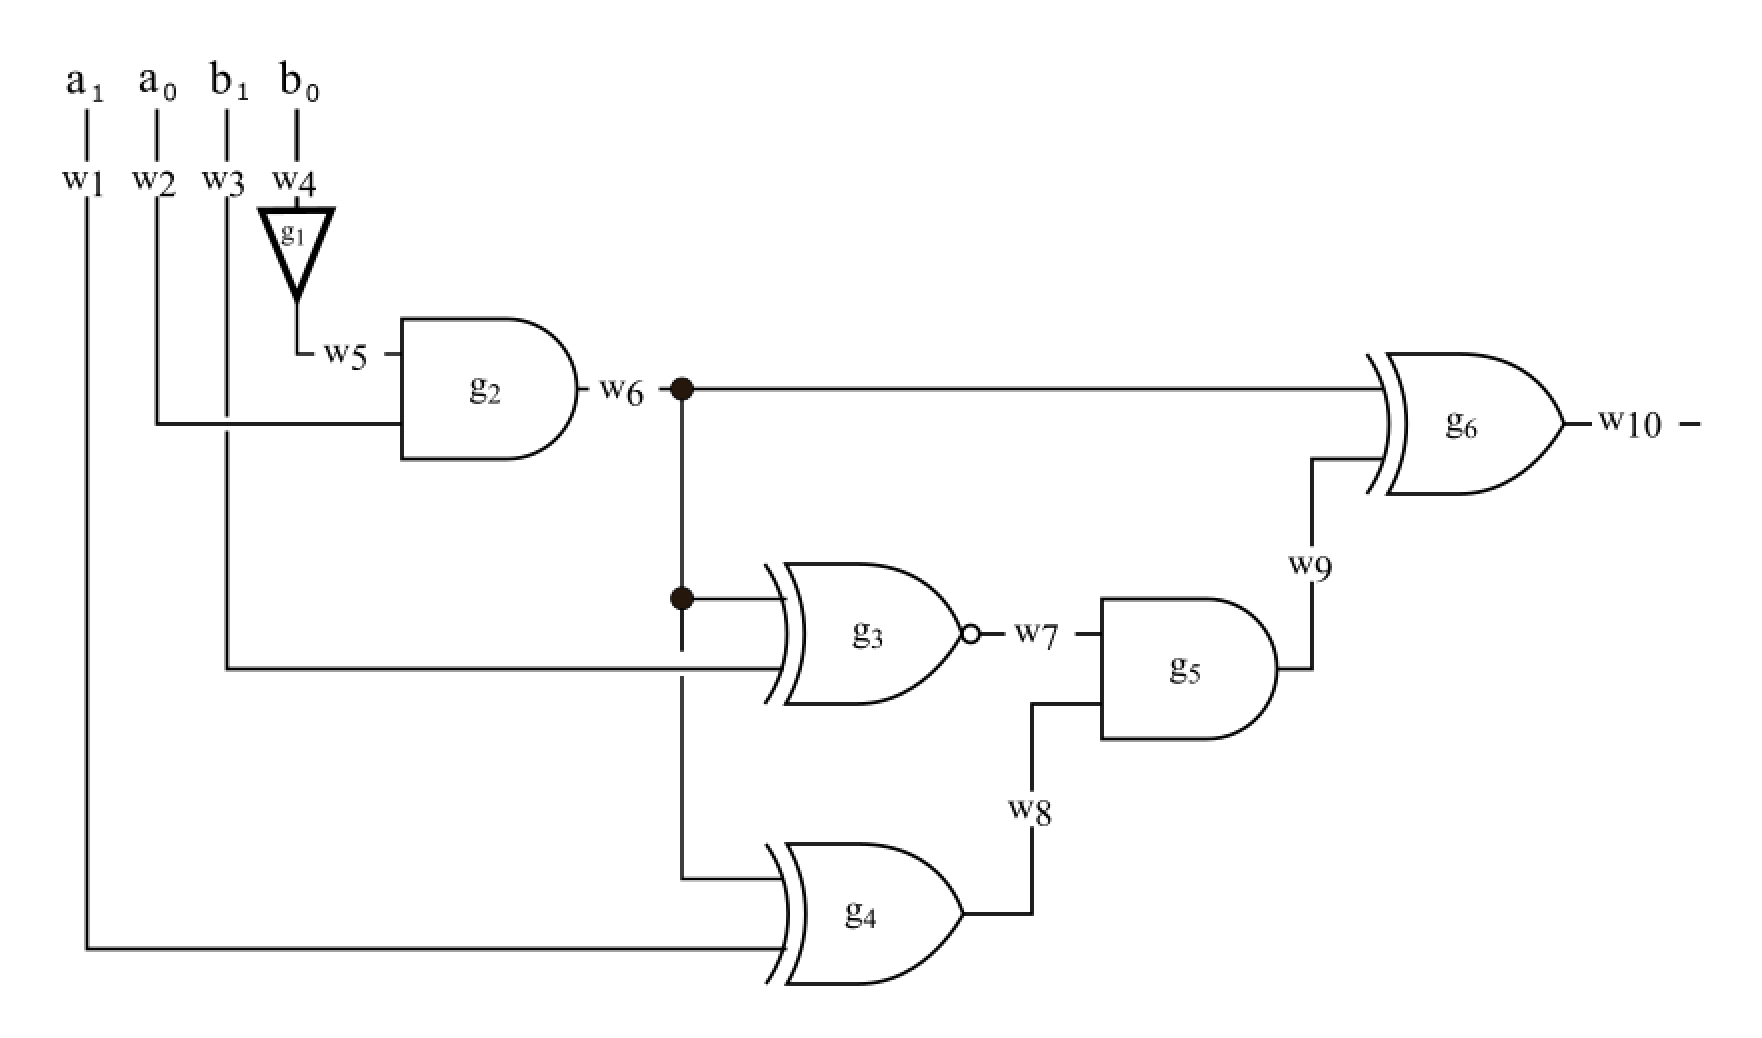
\includegraphics[scale=0.3]{Chapter_TechnicalOverview/booleanCircuit.png}

        \caption{Boolean circuit of the Millionaires' Problem. Optimised circuit according to the construction in \cite{Kolesnikov2009}.}
        \label{fig:boolean}
    \end{figure}
    
    In this case, the circuit contains one NOT gate ($g_1$), two AND gates ($g_2$, and $g_5$), two XOR gate ($g_4$ and $g_6$), one XNOR gate ($g_3$) and four input wires ($w_1$ and $w_2$ belonging to Alice and $w_3$ and $w_4$ to Bob).
    
    \item \textit{Wire encryption:} Alice uses a random number generator to generate two keys $k^0_i$ and $k^1_i$ for each wire $w_i$, $i\in\{1, ..., 10\}$. These keys correspond to the possible values ($0$ or $1$) on the wire. Note that this is done to prevent Bob from knowing the true value of the wires during the evaluation process.
    
    \item \textit{Gate encryption:} For every gate $g_l$ in the circuit with corresponding input wires $w_i$ and $w_j$ and output wire $w_s$, Alice creates the following table:

    \begin{center}
        \begin{tabular}{ |c| } 
        \hline
        $\mathsf{Enc}_{k_i^0}\left(\mathsf{Enc}_{k_j^0}\left(k_s^{g_l(0,0)}\right)\right)$ \\ 
        \hline
        $\mathsf{Enc}_{k_i^0}\left(\mathsf{Enc}_{k_j^1}\left(k_s^{g_l(0,1)}\right)\right)$ \\ 
        \hline
        $\mathsf{Enc}_{k_i^1}\left(\mathsf{Enc}_{k_j^0}\left(k_s^{g_l(1,0)}\right)\right)$ \\ 
        \hline
        $\mathsf{Enc}_{k_i^1}\left(\mathsf{Enc}_{k_j^1}\left(k_s^{g_l(1,1)}\right)\right)$ \\
        \hline
        \end{tabular}
    \end{center}
    
    where $g_l(a,b)$ is the output of gate $g_l$ for inputs $a, b\in \{0, 1\}$. So, we could think of each row as a locked box that requires two keys to be opened. If the two correct keys are used, it outputs the key corresponding to the desired output value given by $g_l$. After encrypting each gate, Alice permutes the rows of the corresponding table, otherwise, it would be easy to know the real value of the input keys. Then, she sends to Bob the garbled tables along with Alice's input keys.
    
    As an example, we can easily see that if we use input keys $k_i^0$ and $k_j^1$ (corresponding to real values $0$ and $1$), we would only be able to decipher the second row of the table, $\mathsf{Enc}_{k_i^0}(\mathsf{Enc}_{k_j^1}(k_s^{g_l(0,1)}))$, and get $k_s^{g_l(0,1)}$.
    
    \item \textit{Oblivious Transfer:} At this stage of the protocol, the evaluator Bob knows the garbled circuit and Alice's input keys but he does not know the keys corresponding to his real inputs. However, since Bob wants to keep his input value private he cannot directly ask for those keys. At this point, the OT functionality enables the evaluator to receive his input keys without compromising neither the evaluator's nor garbler's security. In fact, for every input wire, both parties perform an OT where Alice plays the role of the sender and Bob plays the role of the receiver. 
    
    Let us assume Alice's input keys to be $k_1^0$ and $k_2^1$ (corresponding to the real value  $01$) and Bob's input bits to be $11$. This means that Bob must use the respective input keys ($k_3^1$ and $k_4^1$) in order to correctly evaluate the circuit. So, they will execute two OT protocols where:
    
    \begin{itemize}
        \item Alice inputs: $(k_3^0, k_3^1)$ and $(k_4^0, k_4^1)$;
        \item Bob inputs: $b_1 = 1$ and $b_2 = 1$.
    \end{itemize}
    
    \item \textit{Evaluation:} Once the evaluator has all the necessary elements, he can proceed with the circuit evaluation. In this step, he simply has to decipher the correct rows of the garbled tables sent by Alice with the corresponding keys. Since the rows of the tables are shuffled, the evaluator does not know which row is the correct one. This small issue can be solved by simple techniques (Point-and-Permute or encryption with a certain number of $0$ padded) which, for the sake of brevity, we will not explore here. At the end of the evaluation, the evaluator receives the key that corresponds to the result. Finally, the evaluator sends the resulting key to the garbler and the garbler tells him the final bit.
    
    According to our Millionaires' problem, the evaluation yields the following results for $a = 01$ and $b = 11$: $g_1(k_4^1) = k_5^0$, $g_2(k_5^0, k_2^1) = k_6^0$, $g_3(k_6^0, k_3^1) = k_7^0$, $g_4(k_6^0, k_1^0) = k_8^1$, $g_5(k_7^0, k_8^1) = k_9^0$, $g_6(k_6^0, k_9^0) = k_{10}^0$. Actually, the desired result is $0$.
    
\end{enumerate}


The Yao protocol has its security based on two main building blocks: garbled circuits and oblivious transfer. Although garbled circuits can be generated with symmetric encryption (i.e. using double AES encryption), OT protocols cannot be classically achieved with symmetric cryptography alone \citep{IR89}. Thus, it is crucial to find efficient protocols for a quantum-resistant OT.

%Lindell and Pinkas presented a simulation-based proof that is based on the fact that 
%LP09


%Description
%
%Optimizations
%
%Security
%
%Generalizations of Yao: GMW, BMR

\subsection{Secret sharing approach}

The secret sharing approach, first introduced by BGW \cite{BGW88} and CCD \cite{CCD88}, does not involve encrypting the circuit. Instead, parties use a secret sharing scheme to evaluate the circuit. This approach involves simple operations such as addition and multiplication, but the number of communication rounds needed will depend on the size of the circuit being evaluated. An important primitive for secret sharing based protocols is oblivious linear evaluation (OLE).

\subsubsection{Oblivious linear evaluation}

Oblivious linear evaluation (OLE) can be thought of as a generalization of oblivious transfer (OT) \cite{Rabin81}. It has been shown to be a building block for securely evaluating arithmetic circuits, such as in \cite{AIK11,DKMQ12,GNN17,DGNBNT17}. Specifically, OLE can be used to generate multiplication triples, which are essential for securely computing multiplication gates \cite{DGNBNT17}. OLE also has applications in tasks such as two-party secure computation \cite{IPS09,ADINZ17,BCGI18,HIMV19,CDIKLOV19} and private set intersection \cite{GN19}.


\begin{figure}[h!]
\centering
\begin{tcolorbox}[enhanced, 
                        frame hidden,
                        ]
                        
    \centerline{$\mathcal{F}_{\textbf{OLE}}$ \textbf{functionality}}
            
    \
    
    \begin{itemize}
    		\item \textbf{Input phase:} Alice sends $(a,b)\in\mathbb{Z}_d^2$ (two field elements) to $\mathcal{F}_{\textbf{OLE}}$ and Bob sends $x\in\mathbb{Z}_d$ to $\mathcal{F}_{\textbf{OLE}}$.
    		\item \textbf{Output phase:} Alice receives nothing $\bot$ from the functionality and Bob receives $f(x):= ax + b$.
    \end{itemize}
    
\end{tcolorbox} 
    \caption{OLE functionality.}
    \label{fig:OLE_functionality}
\end{figure}

The OLE functionality specification is presented in Figure~\ref{fig:OLE_functionality}. Similarly, we have that OLE must satisfy the following security requirements:

\begin{itemize}
	\item Concealing: Alices knows nothing about Bob's field element $x$.
	\item Obliviousness: Bob knows nothing about the function $f()$ other than its evaluation at $x$, i.e. $f(x)$.
\end{itemize}

We can also generalize the OLE functionality to a vectorized version. The vector OLE (VOLE) functionality is presented in Figure~\ref{fig:VOLE_functionality}. Note that Bob only inputs one field element $x$ and Alice inputs two vectors. 


\begin{figure}[h!]
\centering
\begin{tcolorbox}[enhanced, 
                        frame hidden,
                        ]
                        
    \centerline{$\mathcal{F}_{\textbf{VOLE}}$ \textbf{functionality}}
            
    \
    
    \begin{itemize}
    		\item \textbf{Input phase:} Alice sends $(\bm{a},\bm{b})\in\mathbb{Z}_d^{2n}$ (two vectors of field elements) to $\mathcal{F}_{\textbf{VOLE}}$ and Bob sends only $x\in\mathbb{Z}_d$ to $\mathcal{F}_{\textbf{VOLE}}$.
    		\item \textbf{Output phase:} Alice receives nothing $\bot$ from the functionality and Bob receives $\bm{f}(x):= \bm{a}x + \bm{b}$.
    \end{itemize}
    
\end{tcolorbox} 
    \caption{VOLE functionality.}
    \label{fig:VOLE_functionality}
\end{figure}


\subsubsection{Basic operations}

To highlight the importance of OLE in secret sharing based SMC protocols, we go through a passively secure protocol \cite{Evans2018}. We consider the two party case (Alice and Bob) where the parties own additive shares of the secret. So, for some secret value $x$, Alice owns $x_A$, Bob owns $x_B$ and $x = x_A + x_B$. Depending on the circuit, the operations used in the protocol are as follows:

\begin{itemize}
	\item \textbf{Input}. For Alice to secret share her input value $x$, she randomly chooses $x_B$ and sends it to Bob. Alice defines $x_A$ as $x_A = x - x_B$;
	\item \textbf{Addition}. There are two scenarios to consider:
	\begin{itemize}
		\item \textbf{Scalar}. For Alice and Bob to add a scalar to a secret $x$ ($z = a + x$), Alice computes $z_A = a + x_A$ and Bob sets $z_B = x_B$.
		\item \textbf{Shares}. For Alice and Bob to add secrets $x$ and $y$ ($z = x+y$), they individually add their corresponding shares, i.e. $z_A = x_A + y_A$ and $z_B = x_B + y_B$.
	\end{itemize}
	\item \textbf{Multiplication}. There are two scenarios to consider:
		\begin{itemize}
		\item \textbf{Scalar}. For Alice and Bob to multiply a secret by a scalar $x$ ($z = a \cdot x$), Alice computes $z_A = a \cdot x_A$ and Bob computes $z_B = a \cdot x_B$.
		\item \textbf{Shares}. Observe that, for Alice and Bob to multiply secrets $x$ and $y$ ($z = x\cdot y$), they require some sort of communication to compute cross terms:
		\begin{eqnarray}
		x\cdot y &=& (x_A + x_B)\cdot (y_A + y_B)\\
		&=& x_A\cdot y_A + x_A\cdot y_B + x_B \cdot y_A + x_B\cdot y_B
		\end{eqnarray}
		
		At this point, Alice and Bob can execute two OLE s to secret share the cross terms $x_A\cdot y_B$ and $x_B \cdot y_A$. Indeed, if Alice inputs $(x_A, - s_A)$ and $(y_A, - s'_A)$ for random values $s_A, s'_A$ and Bob inputs $y_B$ and $x_B$, Bob will output $s_B = x_A \cdot y_B - s_A$ and $s'_B = y_A \cdot x_B - s'_A$. Thus, we have that $s_A + s_B = x_A \cdot y_B$ and $s'_A + s'_B = y_A \cdot x_B$. So, Alice share is $z_A = x_A\cdot y_A + s_A + s'_A$ and Bob share is $z_B =  s_B + s'_B + x_B\cdot y_B$.  
	\end{itemize}
	\item \textbf{Output}. For Alice to receive the output value $x$ of some output wire, Bob simply sends $x_B$ to Alice. Alice outputs $x = x_A + x_B$.
\end{itemize}


%********************************** %Second Section  **************************************
\section{Quantum information}

Quantum information theory is a field that studies the implications of using quantum systems as the medium of information. The information carriers in quantum systems are governed by the laws of quantum mechanics, allowing for properties not present in classical methods to be exploited. In this section, we present the basic elements of quantum information that will be used in the quantum protocols presented and their security proofs.

In quantum information theory, a quantum system is described by a Hilbert space $\mathcal{H}_A$. In this thesis, we will consider only finite-dimensional Hilbert spaces, where $\dim \mathcal{H}_A = d < \inf$. The space $\mathcal{H}_A$ can be identified with the complex vector space $\mathbb{C}^d$, as well as its corresponding dual space $\mathcal{H}^{*}_A$. We use the Dirac bra-ket notation to describe the states of a quantum system. A pure state is described by a normalized vector $\ket{\psi}_A \in \mathcal{H}_A$ and its dual vector $\bra{\psi}_A \in \mathcal{H}^{*}_A$. To simplify notation, we may omit specifying the Hilbert space to which a state belongs if it is clear from context. The standard basis of $\mathbb{C}^d$ can be identified with the computational basis of $\mathcal{H}_A$, denoted as $\left\{ \ket{i} \right\}_{i=0}^{d-1}$. The joint system of multiple subsystems $\mathcal{H}_1, \ldots, \mathcal{H}_n$ can be described by their tensor product, denoted as $\mathcal{H}_1 \otimes \ldots \otimes \mathcal{H}_n$. The vectors in this joint system are represented as $\ket{\bm{x}} = \ket{x_1} \otimes \ldots \otimes \ket{x_n}$, where $\bm{x} \in \mathbb{Z}_d^n$.

We can generate quantum pure states, denoted as $\ket{\psi_i}\in \mathcal{H}$, according to a probability distribution ${p_i}$. This situation is described by a density operator, denoted as $\rho = \sum_i p_i \ketbra{\psi_i}$, which is commonly referred to as a mixed state. Density operators are positive semi-definite hermitian operators with unitary trace, that is, $\rho \geq 0$ and $\tr \rho = 1$. The set of hermitian operators, positive semi-definite operators and density operators on a Hilbert space $\mathcal{H}$ are denoted as $\text{Herm}(\mathcal{H})$, $\text{Pos}(\mathcal{H})$ and $\mathcal{P}(\mathcal{H})$ respectively.

A mixed state is considered classical if it is of the form $\rho_{\mathcal{X}} = \sum_{x\in\mathcal{X}} P_X(x)\ketbra{x}$, where $\mathcal{X}$ is a finite set and $P_X$ is a probability distribution over $\mathcal{X}$. The uniform distribution over $\mathcal{X}$ is denoted as $\tau_{\mathcal{X}} = \frac{1}{|\mathcal{X}|}\sum_{x\in\mathcal{X}}\ketbra{x}$, where $|\mathcal{X}|$ is the size of $\mathcal{X}$. The identity operator is denoted by $\mathds{1}$. Additionally, for a bipartite quantum state $\rho_{XB}$, it is said to be a classical-quantum state (cq-state for short) if it is of the form $\rho_{XB} = \sum_{x\in \mathcal{X}} P_X(x) \ketbra{x} \otimes \rho^x_{B}$, where $P_X$ is a probability distribution over the finite set $\mathcal{X}$.

\subsection{Trace distance}

Proving the security of quantum protocols requires a method for distinguishing quantum states. Fortunately, there is a useful metric, known as the trace distance, that measures the distinguishability of two quantum states, $\sigma, \rho \in \mathcal{P}(\mathcal{H})$, by any procedure, regardless of efficiency. The trace distance is defined as \cite{U17}
\begin{equation*}
    \delta(\rho,\sigma):=\frac{1}{2}||\rho-\sigma||_1,
\end{equation*}
where $||\cdot||_1$ is the $1-$Schatten norm in the space of bounded operators acting on a Hilbert space. Its name comes from the fact that we can write it using the trace operator as follows
\begin{equation*}
    ||\rho-\sigma||_1=\Tr\left\{\sqrt{(\rho-\sigma)^\dagger(\rho-\sigma)}\right\}.
\end{equation*}

In this work, we will utilize completely positive trace preserving (CPTP) maps. These maps are defined as preserving the normalization of input states and mapping positive operators to positive operators. As a result, they ensure that density operators are mapped to density operators, making them useful in describing all physically possible operations. They will be a key focus in Chapter~\ref{ch:QOLE}, which deals with the quantum oblivious linear evaluation protocol. However, it is important to note that CPTP maps do not increase the distinguishability between quantum states, as proven in Lemma~\ref{lemma:trace_distance}. In other words, the trace distance between two quantum states remains unchanged after being transformed by a CPTP map.

%{\cv Useful links to support this: \href{https://en.wikipedia.org/wiki/Quantum_operation#Kraus_operators}{wiki} and \href{https://courses.cs.ut.ee/all/MTAT.07.024/2018_fall/uploads/notes.pdf}{Unruh lectures} on pag 16 (def of quantum operations) and Lemma 7}

\begin{lemma}[Lemma 7, \cite{U17}]

\begin{enumerate}

    The trace distance has the following properties:

    \item For any CPTP map $\mathcal{E}$ and any $\sigma, \rho \in \mathcal{P}(\mathcal{H})$ we have that
    $$\delta(\mathcal{E}(\sigma), \mathcal{E}(\rho)) \leq \delta(\sigma, \rho).$$
    
    \item Let $\sigma, \sigma' \in \mathcal{P}(\mathcal{H})$ and $\rho \in \mathcal{P}(\mathcal{H}')$. Then,
    $$\delta(\sigma\otimes \rho, \sigma'\otimes \rho) = \delta(\sigma, \sigma').$$
\end{enumerate}

\label{lemma:trace_distance}
\end{lemma}

Although the following lemma is not directly related to the trace distance, it will be used in Chapter~\ref{ch:QOLE} to bound the trace distance between two states.

\begin{lemma}[Corollary 4, \cite{LPTRG13}]
Let $X:=\{x_1, \ldots, x_n\}$ be a list of (not necessarily distinct) values in $[0,1]$ with the average $\mu_X:=\frac{1}{n}\sum_{i=1^n} x_i$. Let $T$ of size $t$ be a random subset of $X$ with the average $\mu_T := \frac{1}{t}\sum_{i\in T} x_i$. Then, for any $\epsilon > 0$, the set $\bar{T} = X\setminus T$ with average $\mu_{\bar{T}} = \frac{1}{n-t}\sum_{i\in K} x_i$ satisfies
$$P\left[ \mu_{\bar{T}} - \mu_T \geq \sqrt{\frac{n(t+1)}{2(n-t)t^2} \log \frac{1}{\epsilon}}  \right] \leq \epsilon.$$
\label{lemma:trace_distance_bound}
\end{lemma}

%%%%%%%%%%%%%%%%%%%%%%%%%%%%%%%%%%%%%%%%%%%%%%%%%%%%%%%%%%%%%%%% HERE

\subsection{Entropy}

Entropy measures are used to quantify the unpredictability of a random variable and the amount of information gained by observing a system. One of the earliest and most widely used classical entropy measures was developed by Shannon in 1948 \cite{S48}. Shannon's entropy measure captures the idea that more predictable events convey less information. The more surprising and unpredictable an event is, the more informative it is. Shannon started by proposing the following function to describe the amount of information an event $A$ has:
$$I(A) = - \log \left( P(A) \right),$$
where $P(A)$ is the probability of event $A$. Shannon's entropy is defined as the average amount of information of all possible events, and, for a discrete random variable X,  is calculated as follows:
$$H(X) = \mathbb{E}\left[ I(X) \right].$$

In the case of a distribution $P(X)$ over the set $\left\{0,1\right\}$ that selects 1 with probability $p$ and 0 with probability $1-p$, the binary entropy is given by the following equation:
$$H(X) = -p \log_2 p - (1-p)\log_2(1-p).$$

Throughout our analysis, we will also frequently use the $d-$ary entropy function, which is a generalization of the standard binary entropy function. However, it should be noted that the $d-$ary entropy does not possess the same operational meaning as the binary entropy measure.

\begin{definition}
For $d\geq 2$, the \textit{d-ary entropy function} $h_d : [0,1]\rightarrow\mathbb{R}$ is given by
$$h_d(x) = x \log_d(d-1) - x \log_d x - (1-x) \log_d (1-x).$$
\label{def:q-ary}
\end{definition}
The $d-$ary entropy is specially useful to bound the size of an important object in coding theory, the Hamming ball. The Hamming ball with radius $\mu$ centered at some point $\bm{r}$ is defined to be the set of vectors $\bm{z}$ at a distance $\mu$ from $\bm{r}$, when the distance is given by the Hamming distance $d_H$. So, we have the following Lemma.

\begin{lemma}[Lemma 5, \cite{V10}]
\label{lemma:hammingBall}
For an integer $d\geq 2$ and $\mu \in [0, 1-\frac{1}{d}]$,
\begin{equation*}
    |\{ \boldsymbol{z}\in \mathbb{Z}_d^{n}: d_H(\boldsymbol{z}, \boldsymbol{r})\leq \mu n \}| \leq d^{h_d(\mu)n}.
\end{equation*}
\end{lemma} 

The $d-$ary entropy is particularly useful in bounding the size of the Hamming ball, an important object in coding theory. The Hamming ball with radius $\mu$ centered at a point $\bm{r}$ is defined as the set of vectors $\bm{z}$ that are a distance of $\mu$ away from $\bm{r}$, as measured by the Hamming distance $d_H$. This is stated in the following lemma.

When proving the security of protocols, it is crucial to understand the worst-case scenario rather than the average behavior. Therefore, the standard binary entropy definitions are not sufficient for securing protocols, and a new measure is needed. This is achieved through the use of min-entropy. Classically, for a finite random variable $X$, where $P(X=x) = p_x$, the min-entropy is defined as:
$$H_{\min}(X) = -\log \max p_x.$$
Operationally, this gives the probability of correctly guessing the element drawn from $X$, when choosing the element $x$ with maximum probability. That is, $P_{\text{guess}} = \max p_x$. This definition can also be extended to cq-states $\rho_{XB}\in\mathcal{P}(\mathcal{H}_A \otimes \mathcal{H}_B)$ as defined in Definition~\ref{def:cqentropy}.

\begin{definition}
\label{def:cqentropy}
Let $\rho_{X B}\in\mathcal{P}(\mathcal{H}_X \otimes \mathcal{H}_{B})$ be a cq-state. The conditional min-entropy is given by
$$H_{\min}(X|B)_{\rho} = -\log P_{\text{guess}}(X|B),$$
where $P_{\text{guess}}(X|B)$ is given by
$$P_{\text{guess}}(X|B) = \max_{\{M_x\}_x} \sum_x p_x \tr\left[M_x \rho_{x}^B\right],$$
where the maximization is taken over all positive operator-valued measures (POVM), i.e. $\left\{ M_x \geq 0 : \sum_x M_x = \mathds{1} \right\}$.
\end{definition}

In Definition~\ref{def:cqentropy}, $P_{\text{guess}}(X|B)$ represents the probability of correctly guessing $x$ given access to system $B$. Additionally, the maximization is taken over the most general type of measurements allowed in quantum mechanics. The following Lemma~\ref{lemma:bijectivefunction} states how min-entropy changes when a fixed bijective function is applied to the classical subsystem of a cq-state. This lemma will be important in the proof of security for the quantum oblivious linear evaluation protocol presented in Chapter~\ref{ch:QOLE}.

\begin{lemma}
Let $\rho_{XB} \in \mathcal{P}(\mathcal{H}_{X}\otimes \mathcal{H}_B)$ be a cq-state and let $f:\mathcal{X} \rightarrow \mathcal{X} $ be a fixed bijective function. Then,
$$H_{\min}(X|B)_{\rho} \leq H_{\min}(f(X)|B)_{\rho}.$$
\label{lemma:bijectivefunction}
\end{lemma}
\begin{proof}
Consider the unitary operator,
$$U = \sum_x \ketbra{f(x)}{x}.$$ 

We check that $U$ is indeed unitary:
\begin{equation*}
U U^{\dagger} = \left(\sum_x \ketbra{f(x)}{x}\right)\left(\sum_{x'} \ketbra{x'}{f(x')}\right) 
= \sum_x \ketbra{f(x)} = I,
\end{equation*}
where in the last step we used the fact that the function $f$ is a bijection. The same holds for $U^{\dagger}U = I$.

Now, observe the following,
\begin{eqnarray*}
H_{\min}(f(X)|B) &=& -\log \max_{\{M_x\}_x} \sum_x p_x \tr\left[M_x \rho_{f(x)}^B\right]\\
&=& -\log \max_{\{M_x\}_x} \sum_x p_x \tr\left[M_x U \rho_{x}^B U^{\dagger}\right]\\
&=& -\log \max_{\{M_x\}_x} \sum_x p_x \tr\left[U^{\dagger} M_x U \rho_{x}^B \right]. 
\end{eqnarray*}

It is important to note that $\left\{ N_x \right\}_x= \left\{U^{\dagger} M_x U\right\}_x$ is also a POVM, as they are all positive semidefinite operators and they sum up to unity. Therefore, we have that $\left\{U^{\dagger} M_x U\right\}_x$ can only decrease the space of possible POVMs, which is why we have:
$$\max_{{M_x}x} \sum_x p_x \tr\left[U^{\dagger} M_x U \rho{x}^B \right] \leq \max_{{M_x}x} \sum_x p_x \tr\left[ M_x \rho{x}^B \right].$$

This means that, 
\begin{equation*}
H_{\min}(f(X)|B) \geq -\log \max_{\{M_x\}_x} \sum_x p_x \tr\left[ M_x \rho_{x}^B \right] = H_{\min}(X|B).
\end{equation*}
\end{proof}

%In the first (quantum) part of the OLE protocol, Alice and Bob generate several random OLE instances based on expression~\eqref{eq:main_relation} and use them as a resource to generate one final OLE. However, by using entanglement, Bob is allowed to have some limited amount of information on Alice's outputs, i.e. on Alice functions $(a_i, b_i)_{i\in [n]}$. To understand the impact this have on the security of the protocol, we use the concept of \textit{min-entropy}. This quantifies the amount of information Bob has about Alice system $A$ given some (possibly quantum) side information $B'$. This measure of uncertainty has an important operational meaning when Alice's system is classical. We have that $H_{\text{min}}(A|B') = - \log P_{\text{guess}}(A|B')$, where $P_{\text{guess}}(A|B')$ is the probability that of Bob guessing Alice's classical state $A$ maximized over any possible measurement on his state $B'$. Throughout this work, $A$ will encode Alice's functions with space denoted by $\mathcal{G}^n$. We present the formal definition of min-entropy below.

The conditional min-entropy can be generalized to the fully quantum case where both systems are quantum (Definition~\ref{def:conditionalquantumminentropy}).

\begin{definition}
\label{def:conditionalquantumminentropy}
Let $\rho_{A B'} \in \mathcal{P}(\mathcal{H}_A \otimes \mathcal{H}_B')$ and $\sigma_{B'} \in \mathcal{P}(\mathcal{H}_B')$. The \textit{min-entropy} of $\rho_{A B'}$ relative to $\sigma_{B'}$ is given by
$$H_{\text{min}}(A | B')_{\rho|\sigma} = -\log \min\{ \lambda : \lambda \cdot \text{id}_A \otimes \sigma_{B'} \geq \rho_{A B'} \},$$
and 
$$ H_{\text{min}}(A | B')_{\rho} = \sup_{\sigma_{B'}} H_{\text{min}}(A | B')_{\rho|\sigma}.$$
\end{definition}

Furthermore, consider the superposition state $\ket{\phi}{AB'} = \sum{z\in B}\alpha_z\ket{z} \ket{\psi^z}$ for some set $\mathcal{B}$ and arbitrary coefficients $\alpha_z$. We define $\rho_{AB'} = \ketbra{\phi}{AB'}$ and the mixture $\tilde{\rho}{AB'} = \sum_{z\in \mathcal{B}} |\alpha_z|^2 \ketbra{z} \otimes \ketbra{\psi^z}$. The following lemma gives a lower bound on the min-entropy of $\rho_{AB'}$ in terms of the min-entropy of $\tilde{\rho}_{AB'} $.


\begin{lemma}[Lemma 3.1.13, \cite{R06}]
Let $\rho_{AB'}$ and $\tilde{\rho}_{AB'}$ be defined as above. Then,
$$H_{\text{min}}(A | B')_{\rho} \geq H_{\text{min}}(A | B')_{\tilde{\rho}} - \log |\mathcal{B}|.$$
\label{lemma:renner_lower_bound}
\end{lemma}

It is important to understand the changes in min-entropy that occur when a completely positive (CP) map is applied, as this is a crucial aspect of the security proof for the quantum oblivious linear evaluation protocol outlined in Chapter~\ref{ch:QOLE}. It is known that, for a unital CP map $\mathcal{M}$ (i.e. $\mathcal{M}(\mathds{1}) = \mathds{1}$), the conditional min-entropy does not decrease, i.e. $H_{\min}(\mathcal{M}(A)| B) \geq H_{\min}(A| B)$. However, this result alone is insufficient for deriving practical min-entropy bounds. To obtain meaningful bounds for specific operators $\mathcal{M}$, it is necessary to utilize Theorem~\ref{thm:entaglementSamplingResult}, in conjunction with Lemma~\ref{lemma:quantumrelation} and Lemma~\ref{lemma:classicalquantumrelation}. It is important to note that for clarity, the theorem employs the notation outlined in Chapter~\ref{ch:QOLE}.


\begin{lemma}[Theorem 1, \cite{Dupuis2015}] 
\label{thm:entaglementSamplingResult}
Let $\mathbf{X}$ denote a system with $n$ qudits, and  $\mathcal{M}_{\mathbf{X}\rightarrow \mathbf{F}\mathbf{Y}}$ be a CP map such that $((\mathcal{M}^\dagger \circ \mathcal{M})_{\mathbf{X}}\otimes \text{id}_{\bar{\mathbf{X}}})(\Phi_{\mathbf{X}\bar{\mathbf{X}}}) = \sum_{(\bm{a},\bm{b})\in\mathbb{Z}^{2n}_d} \lambda_{(\bm{a},\bm{b})} \Phi_{(\bm{a},\bm{b})}$. Then, for any partition of $\mathbb{Z}^{2n}_d = \mathfrak{S}_+ \cup \mathfrak{S}_-$ into subsets $\mathfrak{S}_+$ and $\mathfrak{S}_-$, and $\mathcal{M}(\sigma_{\mathbf{X}E}) = \sigma_{\mathbf{F}\mathbf{Y}E}$ we have 
\begin{equation}
    2^{-\text{H}_2(\mathbf{F}\mathbf{Y} | E)_{\sigma_{\mathbf{F}\mathbf{Y}E} | \sigma_{\mathbf{X}E}}} \leq \sum_{(\bm{a},\bm{b})\in\mathfrak{S}_+} \lambda_{(\bm{a},\bm{b})} 2^{-\text{H}_2(\mathbf{X} | E)_{\sigma_{\mathbf{X}E}}} + \left(\max_{(\bm{a},\bm{b})\in\mathfrak{S}_-} \lambda_{(\bm{a},\bm{b})}\right) d^n,
\end{equation}
 where, in general, for a (not necessarily normalized) quantum state $\rho_{AB}\in \mathcal{P}(\mathcal{H}_A\otimes\mathcal{H}_B)$, $\text{H}_2(A|B)$   is the so-called \textit{collision entropy}~\cite{R06}, given as 
\begin{equation*} 
    \text{H}_2(A|B)_{\rho_{AB}}=-\log \left(\Tr{\left(\rho_{B}^{-1/4}\rho_{AB}\rho_B^{-1/4}\right)^2}\right).
\end{equation*}
If we further condition on a general quantum state $\sigma_B\in\mathcal{P}(\mathcal{H}_B)$, we have 
\begin{equation*}
    \text{H}_2(A|B)_{\rho_{AB}|\sigma_B}=-\log \left(\Tr{\left(\sigma_{B}^{-1/4}\rho_{AB}\sigma_B^{-1/4}\right)^2}\right).
\end{equation*}
\end{lemma}

It is interesting to note that when $\mathcal{M}$ is trace preserving, we have,
$$2^{-\text{H}_2(\mathbf{F}\mathbf{Y} | E)_{\sigma_{\mathbf{F}\mathbf{Y}E} | \sigma_{\mathbf{X}E}}} = 2^{-\text{H}_2(\mathbf{F}\mathbf{Y} | E)_{\sigma_{\mathbf{F}\mathbf{Y}E}}}.$$
This follows from the definition of the collision entropy and the fact that $\Tr_{\bm{F} \bm{Y}}\left[ \mathcal{M}(\sigma_{\bm{X} E}) \right] = \sigma_{E}$ \citep{Dupuis2015}. 

%% This definition comes from the fact that a a map M is (\mu-)trace-preserving iff M^\dagger is (\mu-)unital

% Talk a bit about collision entropy. Look at the references here https://arxiv.org/pdf/0807.1338.pdf

Next, we present a chain rule for the collision entropy.

\begin{lemma}[Proposition 8, \cite{MDSFT13}]
For any $\rho_{ABC}\in\mathcal{P}(\mathcal{H}_A\otimes\mathcal{H}_B\otimes\mathcal{H}_C)$, it holds that
$$H_2(A|BC)_{\rho} \geq H_2(AC|B) - \log d_C,$$
where $d_C$ is the rank of $\rho_C$.
\label{lemma:chain_rule}
\end{lemma}

Now, we need a way to relate min-entropy and collision entropy to have useful bounds for min-entropy. This is done through the following two Lemmas.

\begin{lemma}[Lemma 17, \cite{Dupuis2015}]
\label{lemma:quantumrelation}
Let $\rho_{A B'}\in\mathcal{P}(\mathcal{H}_A \otimes \mathcal{H}_{B'})$ and $d_A = \dim\mathcal{H}_A$. Then
$$H_{\min}(A|B')_{\rho} \leq H_2(A|B')_{\rho} \leq 2 H_{\min}(A|B')_{\rho} + \log d_A.$$
\end{lemma}

\begin{lemma}[Lemma 18, \cite{Dupuis2015}]
\label{lemma:classicalquantumrelation}
Let $\rho_{X B'}\in\mathcal{P}(\mathcal{H}_X \otimes \mathcal{H}_{B'})$ be a cq-state. Then
$$H_{\min}(X|B')_{\rho} \leq H_2(X|B')_{\rho} \leq 2 H_{\min}(X|B')_{\rho}.$$
\end{lemma}

Finally, we present a data-processing inequality, which reflects the intuitive idea that the min-entropy of a system $A$, given side information $B$, does not decrease under local physical operations applied to $B$.

\begin{lemma}[Data processing inequality, Theorem 6.19, \cite{T16}]
\label{lemma:data_processing_inequality}
Let $\rho_{A B}\in\mathcal{P}(\mathcal{H}_A \otimes \mathcal{H}_{B})$. Moreover, let $\mathcal{E}$ be a sub-unital CPTP map from system $A$ to $A'$ (i.e. $\mathcal{E}(\mathds{1}_A) \leq \mathds{1}_{A'}$) and $\mathcal{T}$ be a CPTP map from system $B$ to $B'$. Then, the state $\sigma_{A' B'} = \left(\mathcal{E}\otimes \mathcal{T}  \right)\rho_{AB}$ satisfies
$$H_{\min}(A|B)_{\rho}\leq H_{\min}(A'|B')_{\sigma}.$$
\end{lemma}

\subsection{Two-universal functions}

We start by defining a particular set of functions that are usually used to amplify the privacy of the parties' input and output elements. 

\begin{definition}[$\delta-$almost two-universal hash family; two-universal hash family]
A family, $\mathfrak{F}$, of functions, $g$, with domain $D$ and range $R$ is called a $\delta-$almost two-universal hash family if for any two distinct elements $w,w'\in D$ and for $g$ chosen at random from $\mathfrak{F}$, the probability of a \textit{collision} $g(w)=g(w')$ is at most $\delta$. In the special case that $\delta=1/|R|$, where $|R|$ is the size of the range $R$, the family is called \textit{two-universal}. 
\end{definition}

Now, we present a particular two-universal hash family, known as Multi-linear Modular Hashing (MMH), that preserves the structure of the OLE input and output while maintaining its privacy amplification guarantees. This family is based on the modular inner product of vectors \cite{HK97}.
\begin{definition}[Definition 2, \cite{HK97}]
Let $d$ be a prime and let $n$ be an integer $n>0$. Define a family MMH$^*$ (Multi-linear Modular Hashing) of functions from $\mathbb{Z}_d^n$ to $\mathbb{Z}_d$ as follows
$$\text{MMH}^*:= \{ g_x : \mathbb{Z}_d^n\rightarrow \mathbb{Z}_d \, | \, x\in \mathbb{Z}_d^n \},$$
where the functions $g_x$ are defined for any $x = (x_1,\ldots,x_n)$, $m = (m_1,\ldots, m_n) \in \mathbb{Z}_d^n$
$$g_x(m) = x\cdot m \mod d = \sum x_i\, m_i \mod d.$$
\label{def:MMH}
\end{definition}


\begin{theorem}[Theorem 3, \cite{HK97}]
The family MMH$^*$ is two-universal.
\end{theorem}
Halevi and Krawczyk \cite{HK97} actually prove a stronger result, namely that the MMH$^*$ family is \textit{$\Delta-$universal}, which is more general than two-universal. For the sake of simplicity, we only present the simpler version of this theorem here.

The Generalized Leftover Hash Lemma, presented below, is a crucial component in the security proof of Chapter~\ref{ch:QOLE}. It ensures that, after applying a known function $g$ from a two-universal family to a random variable $X$, the resulting random variable $Z = g(X)$ is close to uniform, given some (possibly quantum) side information $E$. This is a high-dimensional version of the Leftover Hash Lemma, which can be easily derived by using Lemma 4 from \cite{TSSR11} with $d_A = d^l$. Note that this is a special version, as Tomamichel et al. in \cite{TSSR11} prove it in the more general case for $\delta-$almost two-universal hash families.

%Next, we state a crucial result that is used to prove the security of the quantum OLE protocol~\footnote{Here we present a multidimensional version of the Generalized Leftover Hash Lemma. This can be easily deduced by using Lemma 4 from Tomamichel et al. work \cite{TSSR11} with $d_A = d$.}. This ensures that, after applying a known function $f$ from a two-universal family to a random variable $X$, the resulting random variable $Z = f(X)$ is close to uniform conditioned on some (possibly quantum) side information $E$. It also describes how close $Z$ is to uniform with respect to the amount of information we have about $X$ conditioned on $E$, i.e. $H_\text{min}(X|E)$.

\begin{lemma}[Generalized Leftover Hash Lemma \cite{TSSR11}]
Let $X$ be a random variable, $E$ a quantum system, and $\mathfrak{F}$ a two-universal family of hash functions from $X$ to $\mathbb{Z}_d^l$. Then, on average over the choices of $g$  from $\mathfrak{F}$, the output $Z := g(X)$ is $\xi$-close to uniform conditioned on $E$, where
\begin{equation}
  \xi = \frac{1}{2}\sqrt{2^{l\log d - H_\text{min}(X|E)}}.  
\end{equation}
 \label{lem:leftover}
\end{lemma}


%********************************** %Third Section  **************************************
\section{Universal composability}

The universal composability (UC) framework, first introduced by Canetti in the classical setting \cite{C20}, was extended to the quantum setting by Unruh, Ben-Or, and Mayers \cite{Unruh04, BenOrMay04} (see also \cite{Unruh10, FS09}). It provides strong composability guarantees by ensuring the security of a protocol is independent of any external execution of the same or other protocols. Both the classical and quantum frameworks use the same ideal-real world comparison structure and consider similar interactions between machines. However, the quantum-UC framework allows for the manipulation of quantum states in addition to classical operations.

Specifically, the quantum-UC security of a protocol $\Pi$ is determined by comparing its execution in a real scenario, where $\Pi$ is executed, to an ideal scenario, where an ideal functionality $\mathcal{F}$ that carries out the same task is executed. The comparison is performed by a special machine called the environment, $\mathcal{Z}$, which supervises the execution of both scenarios and has access to any external information, such as concurrent executions of the same or any other protocol. In the two-party case, the structure of the machines in both scenarios is as follows: in the real scenario, there is the environment $\mathcal{Z}$, the adversary $Adv$, and the two parties, Alice and Bob. In the ideal scenario, there is the environment $\mathcal{Z}$, the simulator $\mathcal{S}$, the two parties Alice and Bob, and the ideal functionality $\mathcal{F}$. Informally, a protocol $\Pi$ is considered quantum-UC secure if the environment $\mathcal{Z}$ cannot distinguish between the execution of $\Pi$ in the real scenario and the execution of the functionality $\mathcal{F}$ in the ideal scenario. Any possible attack of the adversary $Adv$ in the execution of $\Pi$ can be simulated by the simulator $\mathcal{S}$ in the ideal-world execution of $\mathcal{F}$, without any noticeable difference from the point-of-view of the environment $\mathcal{Z}$. As the ideal functionality $\mathcal{F}$ is secure by definition, the real-world adversary is not able to extract any more information than what is allowed by the functionality $\mathcal{F}$.

The formal definition of quantum-UC security can be stated as follows. Let $\Pi$ and $\rho$ represent the real and ideal two-party protocols, respectively. Let $\text{EXEC}{\Pi^C, Adv, \mathcal{Z}}$ denote the output of the environment $\mathcal{Z}$ at the end of the real execution, where $C$ denotes the corrupted party and $Adv$ denotes the adversary. Similarly, let $\text{EXEC}{\rho^C, \mathcal{S}, \mathcal{Z}}$ denote the output of the environment $\mathcal{Z}$ at the end of the ideal execution, where $\mathcal{S}$ is the simulator. 

\begin{definition}[Statistical quantum-UC security,  Computational quantum-UC security \cite{Unruh10}]

Let protocols $\pi$ and $\rho$ be given. We say that $\pi$ statistically quantum-UC emulates $\rho$ if and only if for every party, $C$, and for every adversary, $Adv$, there exists a simulator, $\mathcal{S}$, such that for every environment $\mathcal{Z}$, and every $z\in\{0,1\}^*$, $n\in\mathbb{N}$,
\begin{equation*}
    \big|\text{P}[\text{EXEC}_{\Pi^C, Adv, \mathcal{Z}} (n, z) = 1] - \text{P}[\text{EXEC}_{\rho^C, \mathcal{S}, \mathcal{Z}}(n, z) = 1]\big| \leq \mu(n),
\end{equation*}
 where $\mu(n)$ is a negligible function and $n$ is the security parameter. We furthermore require that if $Adv$ is quantum-polynomial-time, so is $\mathcal{S}$. Finally, if we consider quantum-polynomial-time $Adv$ and $\mathcal{Z}$ we have \textit{computational} quantum-UC security.
\label{def:statisticalquc}
\end{definition}



The role of the simulator, $\mathcal{S}$, in the quantum-UC framework is to simulate the execution of the protocol $\Pi$ in such a way that the environment $\mathcal{Z}$ is not able to distinguish between the real execution and the ideal execution. To accomplish this, $\mathcal{S}$ runs a simulated honest party that interacts with the environment, which is acting as the adversary. Additionally, $\mathcal{S}$ controls the dishonest party and their inputs to the ideal functionality $\mathcal{F}$, as well as the external functionality $\mathcal{F}_{\textbf{ext}}$ if used in the real execution.

In order to generate a simulated execution that cannot be distinguished by the environment, $\mathcal{S}$ relies on its ability to extract the inputs provided to the dishonest party by the environment and uses them along with the ideal functionality outputs. Furthermore, $\mathcal{S}$ can reprogram $\mathcal{F}_{\textbf{ext}}$ in the ideal world as needed to produce an indistinguishable simulation of the real world.

In summary, the simulator $\mathcal{S}$ plays a crucial role in the quantum-UC framework by simulating the execution of the real protocol $\Pi$ in the ideal scenario, in order to ensure that the environment $\mathcal{Z}$ is not able to distinguish between the real execution and the ideal execution, thereby providing strong composability guarantees for the protocol $\Pi$.


%\begin{figure}[!htb]
%\minipage{0.32\textwidth}
%\centering
%  \includegraphics[width=4cm]{img/Real_net.png}
%  \caption{Real model.}\label{fig:realmodel}
%\endminipage\hfill
%\minipage{0.32\textwidth}
%\centering
%  \includegraphics[width=4cm]{img/Ideal_net.png}
%  \caption{Ideal model.}\label{fig:idealmodel}
%\endminipage\hfill
%\minipage{0.32\textwidth}%
%\centering
%  \includegraphics[width=4cm]{img/Real_net.png}
%  \caption{Simulator.}\label{fig:simulator}
%\endminipage
%\end{figure}


 
%Regarding the adversarial model, we consider both \textit{semi-honest} and \textit{dishonest} adversaries. Semi-honest adversaries (also called honest-but-curious or passive adversaries) do not deviate from the protocol and only try to passively gain extra information by looking at the exchanged messages. Dishonest adversaries may deviate arbitrarily from the protocol. We also adopt the static corruption adversarial model where the corruption of each party is done just before the execution of the protocol.


\subsubsection{Ideal functionalities}\label{functinalities}

Whenever a protocol $\Pi$ utilizes an external functionality $\mathcal{F}_{\textbf{ext}}$, we say that $\Pi$ is in the $\mathcal{F}_{\textbf{ext}}-$hybrid model. The quantum OLE protocol $\Pi_{\textbf{QOLE}}$ presented in Chapter~\ref{ch:QOLE} employs the ideal commitment functionality, $\mathcal{F}_{\textbf{COM}}$, defined in Figure~\ref{fig:func_com}. Note that the protocol makes multiple calls to $\mathcal{F}_{\textbf{COM}}$ and only opens a subset of the committed elements. To specify different instance calls, we use an index element $i$. In the commitment phase, Bob sends $(\texttt{commit}, i, M)$ to the functionality, which in turn sends $(\texttt{commit}, i)$ to Alice. In the opening phase, Bob sends $(\texttt{open}, i)$, and the functionality sends $(\texttt{open}, i, M)$ to Alice.

The $\mathcal{F}_{\textbf{COM}}$ functionality can be replaced by the commitment protocol $\Pi_{\textbf{COM}}$ presented in \cite{CF01}, which is computationally UC-secure in the Common Reference String (CRS) model. As analyzed in \cite{CBGLM21} (Theorem 3.), the protocol $\Pi_{\textbf{COM}}$ computationally quantum-UC realizes $\mathcal{F}_{\textbf{COM}}$ in the CRS model. Therefore, since $\Pi_{\textbf{QOLE}}$ is proved to be quantum-UC secure, the resulting protocol $\Pi_{\textbf{QOLE}}^{\Pi_{\textbf{COM}}}$ is quantum-UC secure by the composition theorem \citep{Unruh10}.


%\begin{figure}[!h]
%\centering
%\framebox[\linewidth][l]{%
%    \parbox{0.95\linewidth}{%
%    \begin{center}
%        \textbf{$\mathcal{F}_{\textbf{COM}}$ functionality}
%    \end{center}
%    
%    \textbf{Committer message:} $M$
%    
%    \begin{itemize}
%        \item \textit{Commitment phase}. Upon receiving $( \texttt{commit}, M)$ from Bob, the functionality sends $\texttt{commit}$ to Alice. 
%        \item \textit{Opening phase}. Upon receiving $\texttt{open}$ from Bob, the functionality sends $(\texttt{open}, M)$ to Alice. 
%    \end{itemize}
%    }%
%}
%\caption{Commitment functionality definition.}
%\label{fig:func_com}
%\end{figure}


\begin{figure}[h!]
\centering
\begin{tcolorbox}[enhanced, 
                        frame hidden,
                        ]
                        
    \centerline{$\mathcal{F}_{\textbf{COM}}$ \textbf{functionality}}
            
    \
    
    \begin{itemize}
        \item \textbf{Commitment phase}. Upon receiving $( \texttt{commit}, M)$ from Bob, the functionality sends $\texttt{commit}$ to Alice. 
        \item \textbf{Opening phase}. Upon receiving $\texttt{open}$ from Bob, the functionality sends $(\texttt{open}, M)$ to Alice. 
    \end{itemize}
    
\end{tcolorbox} 
    \caption{Commitment functionality.}
    \label{fig:func_com}
\end{figure}


%\bibliography{bibforthesis}
%\bibliographystyle{unsrt}
%\end{document}

%\documentclass[11pt]{report}



%\begin{document}

\chapter{Quantum oblivious transfer}
\label{chapter_QOT}
%\addcontentsline{toc}{chapter}{Introduction}


In a recent survey on classical oblivious transfer (OT) \cite{YAVV22}, all the analysed protocols require some form of asymmetric cryptography. Indeed, in the classical setting, it is impossible to develop information-theoretic secure OT or even reduce it to one-way functions, requiring some public-key computational assumptions. As shown by Impaggliazzo and Rudich \cite{IR89}, one-way functions (symmetric cryptography) alone do not imply key agreement (asymmetric cryptography). Also, Gertner et al. \cite{GKMRV00} pointed out that since it is known that OT implies key agreement, this sets a separation between symmetric cryptography and OT, leading to the conclusion that OT cannot be generated alone by symmetric cryptography. Otherwise, one could use one-way functions to implement key agreement through the OT construction. This poses a threat to all classical OT protocols \cite{EGL85, NP01, CO15} that are based on mathematical assumptions provably broken by a quantum computer \cite{Sho95}. Besides the security problem, asymmetric cryptography tends to be computationally more complex than symmetric cryptography, creating a problem in terms of speed when a large number of OTs are required. The classical post-quantum approach, thrives to find protocols resistant against quantum computer attacks. However, these are still based on complexity problems and are not necessarily less computationally expensive, than the previously mentioned ones. 

In parallel to the classical post-quantum approach, the quantum cryptography community tackled this security issue by presenting some OT protocols based on quantum technologies. Intriguingly enough, more than a decade before the first classical OT by Rabin (1981, \cite{Rabin81}) was published, Wiesner proposed a similar concept. However, at the time, it was rejected for publication due to the lack of acceptance in the research community. The first published quantum OT (QOT) protocol, known as the BBCS (Bennett-Brassard-Cr{\'e}peau-Skubiszewska) protocol \cite{BBCS92} was only presented in 1992. Remarkably, there is a distinctive difference between classical and quantum OT from a security standpoint, as the latter is proved to be possible assuming only the existence of quantum-hard one-way functions \cite{GLSV21, BCKM21}. This means quantum OT requires weaker security assumptions than classical OT.

In this chapter, we review the particular topic of quantum OT. We mainly comment on several important OT protocols, their underlying security models and assumptions. To the best of our knowledge, there is no prior survey dedicated to quantum OT protocols alone. Usually, its analysis is integrated into more general surveys under the topic of ``quantum cryptography", leading to a less in-depth exposition of the topic. For reference, we provide some distinctive reviews on the general topic of quantum cryptography \cite{BC96, B05, M06, F10, B15, PAB+20, PR21, SH22}.

This chapter is divided as follows. We start by giving a brief overview of the impossibility results related to quantum OT. Then, we provide an exposition about some of the most well-known quantum OT protocols based on assumptions. Finally, we give a brief overview of OT protocols not covered throughout this thesis.

%********************************** %First Section  **************************************
\section{Impossibility results}

The beginning of the development of quantum OT (QOT) came hand in hand with the development of quantum bit commitment (QBC). In fact, the first proposed QOT protocol (BBCS \cite{BBCS92}) reduces QOT to QBC . This sets a distinctive difference between classical and quantum protocols. Although bit commitment (BC) can be reduced to oblivious transfer (OT) \cite{K88}, the reverse is not true using only classical communication \cite{S99}. Therefore, Yao's proof \cite{Y95} of BBCS protocol \cite{BBCS92} gives quantum communications the enhanced quality of having an equivalence between QOT and QBC - they can be reduced to each other - a relation that is not known in the classical realm.

At the time of the BBCS protocol, the quest for unconditionally secure QOT was based on the possibility of unconditional secure QBC. A year later, Brassard et al. presented a QBC protocol \cite{BCJL93} named after the authors, BCJL (Brassard-Crépeau-Jozsa-Langlois). However, this work presented a flawed proof of its unconditional security which was generally accepted for some time, until Mayers spotted an issue on it \cite{M96}. Just one year after, Lo and Chau \cite{LC97}, and Mayers \cite{M97} independently proved unconditional QBC to be impossible. Nevertheless, the existence of unconditionally secure QOT not based on QBC was still put as an open question \cite{BC96} even after the so-called no-go theorems \cite{LC97, M97}. However, Lo was able to prove directly that unconditionally secure QOT is also impossible \cite{L97}. He concluded this as a corollary of a more general result that states that secure two-party computations which allow only one of the parties to learn the result (one-side secure two-party computation) cannot be unconditionally secure. Lo's results triggered a line of research on the possibility of two-sided secure two-party computation (both parties are allowed to learn the result without having access to the other party's inputs), which was also proved by Colbeck to be impossible \cite{C07} and extended in subsequent works \cite{BCS12, SSS14, SJFHV13}. For a more in-depth review of the impossibility results presented by Lo, Chau and Mayers, we refer the interested reader to the following works \cite{BCMS97, S99}.

Although the impossibility results have been well accepted in the quantum cryptography community, there was some criticism regarding the generality of the results \cite{Y00, Y02, Y04, C03}. This line of research reflects the view put forward by Yuen \cite{Y00} in the first of these papers: ``Since there is no known characterization of all possible QBC protocols, logically there can really be no general impossibility proof, strong or not, even if it were indeed impossible to have an unconditionally secure QBC protocol.'' In parallel, subsequent analyses were carried out, reaffirming the general belief of impossibility \cite{B01, C05, Che07}. However, most of the discord has ended with Ariano et al. proof \cite{A07} in 2007, giving an impossibility proof covering all conceivable protocols based on classical and quantum information theory. Subsequent work digested Ariano et al. \cite{A07} work, trying to present more succinct proofs \cite{CAP10, CAPSW13, H13} and to translate it into categorical quantum mechanics language \cite{K12, SHW20, BK22}. 

Facing these impossibility results, the quantum cryptography community followed two main paths:

\begin{enumerate}
    \item Develop OT protocols under some assumptions. These could be based on limiting the technological power of the adversary (e.g. noisy-storage model, relativistic protocols, isolated-qubit model) or assuming the security of additional functionalities (e.g. bit commitment).
    \item Develop OT protocols with a relaxed security definition. These allow the adversary to extract, with a given probability, some information (partial or total) about the honest party input/output. This approach leads to the concepts of weak OT  and weak private database query.
\end{enumerate}

In the next section, we explore protocols that produce a special primitive called \textit{oblivious keys} as an intermediate step.


%********************************** %Second Section  **************************************
\section{BBCS-based protocols}

In this section, we explore protocols that circumvent the no-go theorems \cite{LC97, M97} through assumptions. Some of the presented solutions are based on one-way functions, which are believed to be quantum-hard \cite{BCKM21, GLSV21,A02}, and others rely on technological or physical limitations of the adversaries \cite{DFSS05, WST08, KWW12, L14, Pit16, Ken11}. The latter are qualitatively different from complexity-based assumptions on which post-quantum protocols rely. Also, all these assumptions have the important property that they only have to hold during the execution of the protocol for its security to be preserved. In other words, even if the assumptions lose their validity at some later point in time, the security of the protocol is not compromised. This property is commonly known as \textit{everlasting} security \cite{U18}. Everlasting security is also a major distinctive feature of quantum protocols when compared with classical cryptographic approaches.

We start by presenting the first QOT protocol. Then, we see how this protocol led to the development of two assumption models: $\mathcal{F}_{\text{COM}}-$hybrid model and the limited-quantum-storage model. 

\subsection{BBCS protocol}\label{sec:BBCS}

In 1983, Wiesner came up with the idea of \textit{quantum conjugate coding} \cite{W83}. This technique is the main building block of many important quantum cryptographic protocols \cite{BB84, BBBW83, DFSS14}, including quantum oblivious transfer \cite{BBCS92}. It also goes under the name of \textit{quantum multiplexing} \cite{BBBW83}, \textit{quantum coding} \cite{BBB14} or \textit{BB84 coding} \cite{S99}. In quantum conjugate coding we encode classical information in two conjugate (non-orthogonal) bases. This allows us to have the distinctive property that measuring on one basis destroys the encoded information on the corresponding conjugate basis. So, when bit $0$ and $1$ are encoded by these two bases, no measurement is able to perfectly distinguish the states. We will be using the following bases in the two-dimensional Hilbert space $\mathcal{H}_2$:

\begin{itemize}
    \item Computational basis: $+ := \left\{\ket{0}_{+}, \ket{1}_{+}\right\}$;
    \item Hadamard basis: $\times := \left\{\ket{0}_{\times}, \ket{1}_{\times}\right\} = \left\{\frac{1}{\sqrt{2}}\big( \ket{0}_{+} + \ket{1}_{+} \big), \frac{1}{\sqrt{2}}\big( \ket{0}_{+} - \ket{1}_{+} \big) \right\}$.
\end{itemize}

Throughout this chapter we abuse the notation and consider that the set of bases $\{+,\times\}$ can be associated with the binary set $\{0,1\}$. $+$ is associated with $0$ and $\times$ with $1$. This is specially useful to compare strings of bases from different parties, i.e. the XOR operation ($\oplus$) between two vectors $\bm{\theta}^{\mathsf{A}}, \bm{\theta}^{\mathsf{B}} \in\{+,\times\}^n$ is defined as the XOR between the corresponding binary vectors $\bm{\theta}^{\mathsf{A}}, \bm{\theta}^{\mathsf{B}} \in\{0,1\}^n$.

\

\noindent\textbf{Protocol \cite{BBCS92}.} The first proposal of a quantum oblivious transfer protocol is presented in Figure~\ref{fig:BBCS} and it is called after its creators, Bennett-Brassard-Cr{\'e}peau-Skubiszewska (BBCS). It builds on top of the quantum conjugate coding technique. Alice starts by using this encoding to generate a set of qubits that are subsequently randomly measured by Bob. These two steps make up the first phase of the BB84 QKD protocol. For this reason, this is called the \textit{BB84 phase}. Next, both parties use the output bits obtained from Bob and the random elements generated by Alice to share a special type of key, known as \textit{oblivious key}. This is achieved when Alice reveals her bases $\bm{\theta}^{\mathsf{A}}$ to Bob. Using the oblivious key as a resource, Alice can then obliviously send one of the messages $m_0, m_1$ to Bob, ensuring that he is only able to know one of the messages. This is achieved using a two-universal family of hash functions $\mathfrak{F}$ from $\{0,1\}^{n/2}$ to $\{0,1\}^{l}$. Recall, we use the notation $s\leftarrow_{\$}S$ to describe a situation where an element $s$ is drawn uniformly at random from the set $S$.

\begin{figure}[h!]
    \centering
        \begin{tcolorbox}[enhanced, 
                        frame hidden,
                        ]
            
            \centerline{$\Pi^{\textbf{BBCS}}$ \textbf{protocol}}
            
            \
            
            \textbf{Parameters:} $n$, security parameter; $\mathfrak{F}$ two-universal family of hash functions.
            
            \textbf{Alice's input:} $(m_0, m_1)\in\{0,1\}^l$ (two messages). 
            
            \textbf{Bob's input:} $b\in\{0,1\}$ (bit choice).
            
            \
            
            \textit{BB84 phase}:
            \begin{enumerate}
                \item Alice generates random bits $\bm{x}^{\mathsf{A}}\leftarrow_{\$}\{0,1\}^n$ and random bases $\bm{\theta}^{\mathsf{A}}\leftarrow_{\$}$~$\{+,\times\}^n$. Sends the state $\ket{\bm{x}^{\mathsf{A}}}_{\bm{\theta}^{\mathsf{A}}}$ to Bob.
                \item Bob randomly chooses bases $\bm{\theta}^{\mathsf{B}}\leftarrow_{\$}$~$\{+,\times\}^n$ to measure the received qubits. We denote by $\bm{x}^{\mathsf{B}}$ his output bits.
            \end{enumerate}
            
            \
            
            \textit{Oblivious key phase}:
            \begin{enumerate}
            \setcounter{enumi}{2}
                \item Alice reveals to Bob the bases $\bm{\theta}^{\mathsf{A}}$ used during the \textit{BB84 phase} and sets his oblivious key to $\mathsf{ok}^{\mathsf{A}}:=\bm{x}^{\mathsf{A}}$.
                \item Bob computes $\mathsf{e}^\mathsf{B} = \bm{\theta}^{\mathsf{B}} \oplus \bm{\theta}^{\mathsf{A}}$ and sets $\mathsf{ok}^{\mathsf{B}}:=\bm{x}^{\mathsf{B}}$.
            \end{enumerate}
            
            \
            
            \textit{Transfer phase}:
            \begin{enumerate}
            \setcounter{enumi}{4}
                \item Bob defines $I_0 = \{ i : \mathsf{e}^{\mathsf{B}}_i = 0 \}$ and $I_1 = \{ i : \mathsf{e}^{\mathsf{B}}_i = 1 \}$ and sends the $(I_b, I_{b\oplus 1})$ to Alice.
                \item Alice picks two uniformly random hash functions $f_0, f_1 \in \mathfrak{F}$, computes the pair of strings $(s_0, s_1)$ as $s_i = m_i \oplus f_i(\mathsf{ok}^{\mathsf{A}}_{I_{b\oplus i}})$ and sends the pairs $(f_0, f_1)$ and $(s_0, s_1)$ to Bob.
                \item Bob computes $m_b = s_b \oplus  f_i(\mathsf{ok}^{\mathsf{B}}_{I_0})$. 
            \end{enumerate}
            
            \
            
        \textbf{Alice's output:} $\bot$.
        
        \textbf{Bob's output:} $m_b$.
        
        \end{tcolorbox}
    \caption{BBCS OT protocol.}
    \label{fig:BBCS}
\end{figure}

\

\noindent\textbf{Oblivious keys.}  As we saw in the BBCS protocol, oblivious keys can be used as a resource to produce OT instances. In fact, we can draw a comparison between standard encryption keys and oblivious keys. In the same way as standard keys are the resource that allows the encryption of a specific message, oblivious keys are the resource that enables the performance of OT with messages. In other words, encryption methods consume standard keys, while OT methods consume oblivious keys. The term, oblivious key, was used for the first time by Fehr and Schaffner \cite{FS09} referring to random OT. However, under a subtle different concept, it was put forth by Jakobi et al. \cite{JSGBBWZ11} and used to implement private database queries (PDQ). Also, in a recent work, Lemus et al. \cite{Lemus20} presented the concept of oblivious key applied to OT protocols. We can define it as follows.

\begin{definition}[Oblivious key]
An oblivious key shared between two parties, Alice and Bob, is a tuple $\mathsf{ok}:= \big( \mathsf{ok}^{\mathsf{A}}, (\mathsf{ok}^{\mathsf{B}}, \mathsf{e}^{\mathsf{B}}) \big)$ where $\mathsf{ok}^{\mathsf{A}}$ is Alice's key, $\mathsf{ok}^{\mathsf{B}}$ is Bob's key and $\mathsf{e}^{\mathsf{B}}$ is Bob's signal string. $\mathsf{e}^{\mathsf{B}}$ indicates which indexes of $\mathsf{ok}^{\mathsf{A}}$ and $\mathsf{ok}^{\mathsf{B}}$ are correlated and which indexes are uncorrelated, i.e. $\mathsf{e}^{\mathsf{B}}_i = 0$ when the corresponding indexes are correlated and $\mathsf{e}^{\mathsf{B}}_i = 1$ when they are not.
\label{def:ok}
\end{definition}

Note that, for some index $i$, when two index elements $\mathsf{ok}^{\mathsf{A}}_i$ and $\mathsf{ok}^{\mathsf{B}}_i$ are correlated, $\mathsf{ok}^{\mathsf{A}}_i=\mathsf{ok}^{\mathsf{B}}_i$. However, when they are uncorrelated, they are drawn independently. This means that both index elements may either be equal or different. Consider the following oblivious key $\mathsf{ok}=\left( 001101101101, \left( 000101001100, 101000110001 \right) \right)$ as an example. We can check it is a well strucured oblivious key:

\begin{equation*}
    \left.\begin{array}{cc}
      \mathsf{ok}^{\mathsf{A}} :& \tikzmarkin{a}\red{0}\,\,\,\, \tikzmarkin{b}\green{0}\,\,\,\, \tikzmarkin{c}\red{1}\,\,\,\, \tikzmarkin{d}\green{1}\,\,\,\, \tikzmarkin{e}\green{0}\,\,\,\, \tikzmarkin{f}\green{1}\,\,\,\, \tikzmarkin{g}\red{1}\,\,\,\, \tikzmarkin{h}\red{0}\,\,\,\, \tikzmarkin{i}\green{1}\,\,\,\, \tikzmarkin{j}\green{1}\,\,\,\, \tikzmarkin{k}\green{0}\,\,\,\, \tikzmarkin{l}\red{1}  \\
      \mathsf{ok}^{\mathsf{B}} :& \red{0}\,\,\,\, \green{0}\,\,\,\, \red{0}\,\,\,\, \green{1}\,\,\,\, \green{0}\,\,\,\, \green{1}\,\,\,\, \red{0}\,\,\,\, \red{0}\,\,\,\, \green{1}\,\,\,\, \green{1}\,\,\,\, \green{0}\,\,\,\, \red{0} \\
      \mathsf{e}^{\mathsf{B}} :& \red{1}\tikzmarkend{a}\,\,\,\, \green{0}\tikzmarkend{b}\,\,\,\, \red{1}\tikzmarkend{c}\,\,\,\, \green{0}\tikzmarkend{d}\,\,\,\, \green{0}\tikzmarkend{e}\,\,\,\, \green{0}\tikzmarkend{f}\,\,\,\, \red{1}\tikzmarkend{g}\,\,\,\, \red{1}\tikzmarkend{h}\,\,\,\, \green{0}\tikzmarkend{i}\,\,\,\, \green{0}\tikzmarkend{j}\,\,\,\, \green{0}\tikzmarkend{k}\,\,\,\, \red{1}\tikzmarkend{l}
    \end{array}\right\} \mathsf{ok}
\end{equation*}

It is worth stressing that oblivious keys are independent of the sender's messages  $m_0, m_1$ and are not the same as random OT. In fact, as Alice does not know the groups of indexes $I_0$ and $I_1$ computed by Bob after the basis revelation, Alice does not have her messages fully defined. A similar concept was defined by K\"onig et al.  \cite{KWW12} under the name of \textit{weak string erasure}. 

\

\noindent\textbf{Security.} Regarding security, the BBCS protocol is unconditionally secure against dishonest Alice. Intuitively, this comes from the fact that Alice does not receive any information from Bob other than some set of indexes $I_0$. However, the BBCS protocol is insecure against dishonest Bob. In its original paper \cite{BBCS92}, the authors describe a memory attack that provides Bob complete knowledge on both messages $m_0$ and $m_1$ without being detected. This can be achieved by having the receiver delay his measurements in step 2 to some moment after step 3. This procedure is commonly called the memory attack as it requires quantum memory to hold the states until step 3. The authors suggest that, for the protocol to be secure, the receiver has to be forced to measure the received states at step 2. In the following sections, we present two common approaches to tackle this issue. We may assume the existence of commitments or set physical assumptions that constrain Bob from delaying his measurement.


\subsection{BBCS in the $\mathcal{F}_{\textbf{COM}}-$hybrid model}\label{BBCS-com-hybrid}

As mentioned in the previous section, a secure BBCS protocol requires Bob to measure his qubits in step 2. In this section, we follow the suggestion from the original BBCS paper \cite{BBCS92} and fix this loophole using a commitment scheme. Since we assume we have access to some commitment scheme, we call it $\mathcal{F}_{\textbf{COM}}-$hybrid model\footnote{The notation $\mathcal{F}_{\textbf{COM}}$ is commonly used for ideal functionalities. However, here we abuse the notation by using $\mathcal{F}_{\textbf{COM}}$ to refer to any commitment scheme (including the ideal commitment functionality).}.

\begin{figure}[h!]
\centering
\begin{tcolorbox}[enhanced, 
                        frame hidden,
                        ]
                        
    \centerline{$\Pi^{\textbf{BBCS}}_{\mathcal{F}_{\textbf{COM}}}$ \textbf{protocol}}
            
    \
    
    \textbf{Parameters:} $n$, security parameter; $\mathfrak{F}$ two-universal family of hash functions.
    
    \textbf{Alice's input:} $(m_0, m_1)\in\{0,1\}^l$ (two messages). 
    
    \textbf{Bob's input:} $b\in\{0,1\}$ (bit choice).
    
    \
    
    \textit{BB84 phase:} \textcolor{gray}{Same as in $\Pi^{\textbf{BBCS}}$ (Figure~\ref{fig:BBCS}).}
    
    
    \
    
    \textit{Cut and choose phase}:
    \begin{enumerate}
    \setcounter{enumi}{2}
        \item Bob commits to the bases used and the measured bits, i.e. $\textbf{COM}\big(\bm{\theta}^\mathsf{B}, \bm{x}^\mathsf{B}\big)$, and sends to Alice. %using $\mathcal{F}_{\textbf{com}}$.
        \item Alice asks Bob to open a subset $T$ of commitments (e.g. $n/2$ elements) and receives $\{\theta_i^\mathsf{B}, x_i^\mathsf{B}\}_{i\in T}$.% from $\mathcal{F}_{\textbf{com}}$.
        \item In case any opening is not correct or $x_i^\mathsf{B} \neq x_i^\mathsf{A}$ for $\theta_i^\mathsf{B} = \theta_i^\mathsf{A}$, abort. Otherwise, proceed. 
    \end{enumerate}
    
    \
    
    \textit{Oblivious key phase:} \textcolor{gray}{Same as in $\Pi^{\textbf{BBCS}}$ (Figure~\ref{fig:BBCS}).}
     
    \
     
    \textit{Transfer phase:} \textcolor{gray}{Same as in $\Pi^{\textbf{BBCS}}$ (Figure~\ref{fig:BBCS}).}
    
    \
    
\textbf{Alice's output:} $\bot$.

\textbf{Bob's output:} $m_b$.
    
\end{tcolorbox} 
    \caption{BBCS OT protocol in the $\mathcal{F}_{\textbf{COM}}-$hybrid model.}
    \label{fig:BBCS_COM}
\end{figure}

\noindent\textbf{Protocol.} The modified BBCS (Figure~\ref{fig:BBCS_COM}) adds a \textit{cut and choose} phase that makes use of a commitment scheme \textbf{COM} to check whether Bob measured his qubits in step 2 or not. It goes as follows. Bob commits to the bases used to measure the qubits in the \textit{BB84 phase} and the resulting output bits. Then,Alice chooses a subset of qubits to be tested and asks Bob to open the corresponding commitments of the bases and output elements. If no inconsistency is found, both parties can proceed with the protocol. Note that the size of the testing subset has to be proportional to $n$ (security parameter), as this guarantees that the rest of the qubits were measured by Bob with overwhelming probability in $n$.

\

\noindent\textbf{Security.} Formally proving the security of this protocol led to a long line of research \cite{CK88, BBCS92, MS94, Y95, M96b, CDMS04, FS09, DFLSS09, U10, BF10, GLSV21, BCKM21}. Earlier proofs from the $90$'s started by analyzing the security of the protocol against limited adversaries that were only able to do individual measurements \cite{MS94}. Then, Yao \cite{Y95} was able to prove its security against more general adversaries capable of doing fully coherent measurements. Although these initial works \cite{MS94, Y95, M96b} were important to start developing a QOT security proof, they were based on unsatisfactory security definitions. At the time of these initial works, there was no composability framework \cite{FS09, U10} under which the security of the protocol could be considered. In modern quantum cryptography, these protocols are commonly proved in some quantum simulation-paradigm frameworks \cite{FS09, U10, DFLSS09, KWW12}. In these paradigms, the security is proved by showing that an adversary in a real execution of the protocol cannot cheat more than what he is allowed in an ideal execution, which is secure by definition. This is commonly proved by utilizing an entity, called simulator, whose role is to guarantee that a real execution of the protocol is indistinguishable from an ideal execution. Moreover, they measured the adversary's information through average-case measures (e.g. Collision Entropy, Mutual Information) which are proven to be weak security measures when applied to cryptography \cite{BCC+10, TR11}.

More desirable worst-case measures started to be applied to quantum oblivious transfer around a decade later \cite{R06, DFRSS07}. These were based on the concept of \textit{min-entropy} \cite{BCC+10,TR11}, $H_{\text{min}}$, which, intuitively, reflects the maximum probability of an event to happen. More precisely, in order to prove security against dishonest Bob, one is interested in measuring Bob's min-entropy on Alice's oblivious key $\mathsf{ok}^{\mathsf{A}}$ conditioned on some quantum side information $E$ he may has, i.e. $H_{\text{min}}(\mathsf{ok}^{\mathsf{A}} | E)$. Informally, for a bipartite classical-quantum state $\rho_{X E}$ the conditional min-entropy $H_{\text{min}}(X | E)$ is given by 

$$H_{\text{min}}(X | E)_{\rho_{X E}} := -\log P_{guess}(X|E),$$
where $P_{guess}(X|E)$ is the probability the adversary guesses the value $x$ maximized over all possible measurements. Damg{\aa}rd et al. \cite{DFLSS09} were able to prove the stand-alone QOT security when equipped with this min-entropy measure and with the quantum simulation-paradigm framework developed by Fehr and Schaffner \cite{FS09}. Their argument to prove the security of the protocol against dishonest Bob can be summarized as follows. The cut and choose phase ensures that Bob's conditional min-entropy on the elements of $\mathsf{ok}^{\mathsf{A}}$ belonging to $I_{1}$ (indexes with uncorrelated elements between Alice's and Bob's oblivious keys) is lower-bounded by some value that is proportional to the security parameter, i.e. $H_{\text{min}}(\mathsf{ok}^{\mathsf{A}}_{I_{1}} | E) \geq n\lambda$ for some $\lambda > 0$. Note that this is equivalent to derive an upper bound on the guessing probability $P_{guess}(\mathsf{ok}^{\mathsf{A}}_{I_{1}}|E) \leq 2^{-n\lambda}$. Having deduced an expression for $\lambda$, they proceed by applying a random hash function $f$ from a two-universal family $\mathfrak{F}$, $f\leftarrow_{\$}\mathfrak{F}$. This final step ensures that $f(\mathsf{ok}^{\mathsf{A}}_{I_{1}})$ is statistically indistinguishable from uniform (privacy amplification theorem \cite{DFRSS07, RK05, R05}). The proof provided by Damg{\aa}rd et al. \cite{DFLSS09} was extended by Unruh \cite{U10} to the quantum Universal Composable (UC) model, making use of ideal commitments. Now, a natural question arises: 

\

\centerline{\textit{Which commitment schemes can be used to render simulation-based security?}}

\

\noindent\textbf{Commitment scheme.} The work by Aaronson \cite{A02} presented a non-constructive proof that ``indicates that collision-resistant hashing might still be possible in a quantum setting'', giving confidence in the use of commitment schemes based on quantum-hard one-way functions in the $\Pi^{\textbf{BBCS}}_{\mathcal{F}_{\textbf{COM}}}$ protocol. Hopefully, it was shown that commitment schemes can be built from any one-way function \cite{N91, HILL99, HR07}, including quantum-hard one-way functions. Although it is intuitive to plug in into $\Pi^{\textbf{BBCS}}_{\mathcal{F}_{\textbf{COM}}}$ a commitment scheme derived from a quantum-hard one-way function, this does not necessarily render a simulation-based secure protocol. This happens because the nature of the commitment scheme can make the simulation-based proof difficult or even impossible. For a detailed discussion see \cite{GLSV21}.

Indeed, the commitment scheme must be quantum secure. Also, the simulator must have access to two intriguing properties: \textit{extractability} and \textit{equivocality}. Extractability means the simulator can extract the committed value from a malicious committer. Equivocal means the simulator can change the value of a committed value at a later time. Although it seems counter-intuitive to use a commitment scheme where we can violate both security properties (hiding and biding properties), it is fundamental to prove its security. Extractability is used by the simulator to prove security against the dishonest sender and equivocality is used by the simulator to prove security against the dishonest receiver. In the literature, there have been some proposals of the commitment schemes $COM$ with these properties based on:

\begin{itemize}
    \item Quantum-hard one-way functions \cite{BCKM21, GLSV21};
    \item Common Reference String (CRS) model \cite{U10, CF01};
    \item Bounded-quantum-storage model \cite{U11};
    \item Quantum hardness of the Learning With Errors assumption \cite{DFLSS09}.
\end{itemize}

\

\noindent\textbf{Composability.} The integration of secure OT executions in secure multiparty protocols \cite{Y86} should not lead to security breaches. Although it seems intuitive to assume that a secure OT protocol can be integrated within more complex protocols, proving this is highly non-trivial as it is not clear \textit{a priori} under which circumstances protocols can be composed \cite{MR09}. 

The first step towards composability properties is the development of simulation based-security. However, this does not necessarily imply composability (see Section~$4.2$ of \cite{MR09} for more details), as a composability framework is also required. In the literature, there have been some proposals for such a framework. In summary, Fehr and Schaffner \cite{FS09} developed a composability framework that allows sequential composition of quantum protocols in a classical environment. The works developed by Ben-Or and Mayers \cite{BM04} and Unruh \cite{U04, U10} extended the classical Universal Composability model \cite{C20} to a quantum setting (quantum-UC model), allowing concurrent composability. Maurer and Renner \cite{MR11} developed a more general composability framework that does not depend on the models of computation, communication, and adversary behaviour. More recently, Broadbent and Karvonen \cite{BK22} created an abstract model of composable security in terms of category theory. Up until now, and to the best of our knowledge, the composable security of the protocol $\Pi^{\textbf{BBCS}}_{\mathcal{F}_{\textbf{COM}}}$ was only proven in the Fehr and Schaffner model \cite{FS09} by Damg{\aa}rd et al. \cite{DFLSS09} and in the quantum-UC by Unruh \cite{U10}.



\subsection{BBCS in the limited-quantum-storage model}

In this section, we review protocols based on the limited-quantum-storage model. The protocols developed under this model avoid the no-go theorems because they rely their security on reasonable assumptions regarding the storage capabilities of both parties. Under this model, there are mainly two research lines. One was started by Damg{\aa}rd, Fehr, Salvail and Schaffner \cite{DFSS05}, who developed the bounded-storage model. In this model, the parties can only store a limited number of qubits. The other research line was initiated by Wehner, Schaffner and Terhal \cite{WST08}, who developed the noisy-storage model. In this model the parties can store \textit{all} qubits. However, they are assumed to be unstable, i.e. they only have imperfect noisy storage of qubits that forces some decoherence. In both models, the adversaries are forced to use their quantum memories as both parties have to wait a predetermined time $(\Delta t)$ during the protocol.

\subsection{Bounded-quantum-storage model}

In the bounded-quantum-storage model or BQS model for short, we assume that, during the waiting time $\Delta t$, the adversaries are only able to store a fraction $0< \gamma < 1$ of the transmitted qubits, i.e. the adversary is only able to keep $q = n\gamma$ qubits. The parameter $\gamma$ is commonly called the storage rate.

\

\noindent\textbf{Protocol.} The protocol in the BQS model, $\Pi^{\textbf{BBCS}}_{\textbf{bqs}}$, is very similar to the BBCS protocol $\Pi^{\textbf{BBCS}}$ presented in Figure~\ref{fig:BBCS}. The difference is that both parties have to wait a predetermined time ($\Delta t$) after step 2. This protocol is presented in Figure~\ref{fig:BBCS_Bounded}.

\begin{figure}[h!]
\centering
\begin{tcolorbox}[enhanced, 
                        frame hidden,
                        ]
    
    \centerline{$\Pi^{\textbf{BBCS}}_{\textbf{bqs}}$ \textbf{protocol}}
            
    \
    
    \textbf{Parameters:} $n$, security parameter; $\mathfrak{F}$  two-universal family of hash functions.
    
    \textbf{Alice's input:} $(m_0, m_1)\in\{0,1\}^l$ (two messages). 
    
    \textbf{Bob's input:} $b\in\{0,1\}$ (bit choice).
    
    \
    
    \textit{BB84 phase}: \textcolor{gray}{Same as in $\Pi^{\textbf{BBCS}}$ (Figure~\ref{fig:BBCS}).}
    
    
    \
    
    \textit{Waiting time phase}:
    \begin{enumerate}
    \setcounter{enumi}{2}
        \item Both parties wait time $\Delta t$.
    \end{enumerate}
    
    \
    
    \textit{Oblivious key phase}: \textcolor{gray}{Same as in $\Pi^{\textbf{BBCS}}$ (Figure~\ref{fig:BBCS}).}
     
    \
     
    \textit{Transfer phase}: \textcolor{gray}{Same as in $\Pi^{\textbf{BBCS}}$ (Figure~\ref{fig:BBCS}).}
    
    \
    
\textbf{Alice's output:} $\bot$.

\textbf{Bob's output:} $m_b$.
    
\end{tcolorbox}
    \caption{BBCS OT protocol in the bounded-quantum-storage model.}
    \label{fig:BBCS_Bounded}
\end{figure}

\

\noindent\textbf{Security.} We just comment on the security against dishonest Bob because the justification for the security against dishonest Alice is the same as in the original BBCS protocol, $\Pi^{\textbf{BBCS}}$ (see Section~\ref{sec:BBCS}). 

Under the BQS assumption, the waiting time ($\Delta t$) effectively prevents Bob from holding \textit{a large fraction} of qubits until Alice reveals the bases choices $\bm{\theta}^{\mathsf{A}}$ used during the \textit{BB84 phase}. This comes from the fact that a dishonest Bob is forced to measure a fraction of the qubits, leading him to lose information about Alice's bases $\bm{\theta}^{\mathsf{A}}$.

More specifically, Damg{\aa}rd et al. \cite{DFRSS07} showed that, with overwhelming probability, the loss of information about Alice's oblivious key ($\mathsf{ok}^{\mathsf{A}}_{I_{1}}$) is described by a lower bound on the min-entropy \cite{F10}

$$H_{\text{min}}(\mathsf{ok}^{\mathsf{A}}_{I_{1}} | E) \geq 
\frac{1}{4}n - \gamma n - l - 1.$$
Similarly to the $\mathcal{F}_{\textbf{COM}}-$hybrid model, the min-entropy value has to be bounded by a factor proportional to the security parameter $n$. To render a positive bound, we derive an upper bound on the fraction of qubits that can be saved in the receiver's quantum memory, while preserving the security of the protocol, i.e. $\gamma < \frac{1}{4}$. 

The above upper bound was later improved by K\"onig et al. \cite{KWW12} to $\gamma < \frac{1}{2}$. The authors also showed that the BQS model is a special case of the noisy-quantum-storage model. Subsequently, based on higher-dimensional mutually unbiased bases, Mandayam and Wehner \cite{MW11} presented a protocol that is still secure when an adversary cannot store even a small fraction of the transmitted pulses. In this latter work, the storage rate $\gamma$ approaches $1$ for increasing dimension.

\

\noindent\textbf{Composability.} The initial proofs given by Damg{\aa}rd et al. \cite{DFSS05, DFRSS07} were only developed under the stand-alone security model \cite{WW08}. In this model the composability of the protocol is not guaranteed to be secure. These proofs were extended by Wehner and Wullschleger \cite{WW08} to a simulation-based framework that guarantees sequential composition. Also, in a parallel work, Fehr and Schaffner developed a sequential composability framework under which $\Pi^{\textbf{BBCS}}_{\textbf{bqs}}$ is secure considering the BQS model. 

The more desirable quantum-UC framework was extended by Unruh and combined with the BQS model \cite{U11}. In Unruh's work, he developed the concept of BQS-UC security which, as in UC security, implies a very similar composition theorem. The only difference is that in the BQS-UC framework we have to keep track of the quantum memory-bound used by the machines activated during the protocol. Under this framework, Unruh follows a different approach as he does not use the protocol $\Pi^{\textbf{BBCS}}_{\textbf{bqs}}$ (Figure~\ref{fig:BBCS_Bounded}). He presents a BQS-UC secure commitment protocol and composes it with the $\Pi^{\textbf{BBCS}}_{\mathcal{F}_{\textbf{COM}}}$ protocol (Figure~\ref{fig:BBCS_COM}) in order to get a constant-round protocol that BQS-UC-emulates any two-party functionality.

\

\subsection{Noisy-quantum-storage model}

The noisy-quantum-storage model, or NQS model for short, is a generalization of the BQS model. In the NQS model, the adversaries are allowed to keep any fraction $\nu$ of the transmitted qubits (including the case $\nu=1$) but their quantum memory is assumed to be noisy \cite{KWW12}, i.e. it is impossible to store qubits for some amount of time ($\Delta t$) without undergoing decoherence. 

More formally, the decoherence process of the qubits in the noisy storage is described by a completely positive trace preserving (CPTP) map (also called channel) $\mathcal{C}: \mathcal{P}(\mathcal{H}_{\text{in}})\rightarrow \mathcal{P}(\mathcal{H}_{\text{out}})$, where $\mathcal{H}_{\text{in/out}}$ is the Hilbert space of the stored qubits before (in) and after (out) the storing period $\Delta t$ and $\mathcal{P}(\mathcal{H})$ is the set of positive semi-definite operators with unitary trace acting on an Hilbert space $\mathcal{H}$. $\mathcal{C}$ receives a quantum state $\rho\in \mathcal{H}_{\text{in}}$ at time $t$ and outputs a quantum state $\rho'\in\mathcal{H}_{\text{out}}$ at a later time $t + \Delta t$. %See Figure~\ref{fig:NQS_scheme} for a description of the possible malicious behaviour. 

With this formulation, we can easily see that the BQS model is a particular case of the NQS. In BQS, the channel is of the form $\mathcal{C} = \mathds{1}^{\otimes \nu n}$, where the storage rate $\nu$ is the fraction of transmitted qubits stored in the quantum memory. The most studied scenario is restricted to $n-$fold quantum channels, i.e. $\mathcal{C} = \mathcal{N}^{\otimes \nu n}$ \cite{S10, KWW12, WST08}, where the channel $\mathcal{N}$ is applied independently to each individual stored qubit. In this particular case, it is possible to derive specific security parameters.

%\begin{figure}
%    \centering
%    \includegraphics[scale=.1]{fig/nqs_channel.jpeg}
%    \caption{During waiting times $\Delta t$, the adversary must use his noisy quantum storage described by the CPTP map $\mathcal{C}$. Before using his quantum storage, he performs any (error-free) “encoding attack” of his choosing, which consists of a measurement or an encoding into an error-correcting code. After time $\Delta t$, he receives some additional information that he can use for decoding. Figure taken from \cite{WCSL10}.}
%    \label{fig:NQS_scheme}
%\end{figure}

\

\noindent\textbf{Protocols.} The protocol from BQS model $\Pi^{\textbf{BBCS}}_{\textbf{bqs}}$ is also considered to be secure in the NQS model \cite{S10}. However, the first proposed protocol analysed in this general NQS model was developed by K\"onig et al. \cite{KWW12}. This protocol draws inspiration from the research line initiated by Cachin, Crépeau and Marcil \cite{CCM98} about classical OT in the bounded-classical-storage model \cite{DHRS04, S07}. Similar to these works \cite{CCM98, DHRS04, S07}, the protocol presented by K\"onig et al. \cite{KWW12} uses the following two important techniques in its classical post-processing phase: encoding of sets and interactive hashing. The former is defined as an injective function $\mathsf{Enc}: \{0,1\}^t \rightarrow T$, where $T$ is a set of all subsets of $[n]$ with size $n/4$. The latter is a two-party protocol between Alice and Bob with the following specifications. Bob inputs some message $W^t$ and both parties receive two messages $W^t_0$ and $W^t_1$ such that there exists some $b\in\{0,1\}$ with $W^t_b = W^t$. The index $b$ is unknown to Alice, and Bob has little control over the choice of the other message $W^t$, i.e. it is randomly chosen by the functionality. %A schematic representation of the interactive hashing functionality is given in Figure~\ref{fig:IH}.

%\begin{figure}[h!]
%    \centering
%    \includegraphics[scale=.1]{fig/Interactive_hashing.jpeg}
%    \caption{Interactive hashing functionality. Figure taken %from \cite{KWW12}.}
%    \label{fig:IH}
%\end{figure}

In this section, we only present the na\"ive protocol presented in the original paper \cite{KWW12} as it is enough to give an intuition on the protocol. Although both $\Pi^{\textbf{BBCS}}_{\textbf{bqs}}$ and $\Pi^{\textbf{BBCS}}_{\textbf{nqs}}$ protocols are different, we keep a similar notation for a comparison purpose. The protocol $\Pi^{\textbf{BBCS}}_{\textbf{nqs}}$ (Figure~\ref{fig:BBCS_Noisy}) goes as follows. The first two phases (\textit{BB84} and \textit{Waiting time}) are the same as in $\Pi^{\textbf{BBCS}}_{\textbf{bqs}}$ (Figure~\ref{fig:BBCS_Bounded}). Then, both parties generate a very similar resource to oblivious keys, named \textit{weak string erasure} (WSE). After the WSE generation, Alice also holds the totality of the key $\mathsf{ok}^{\mathsf{A}}$, while Bob holds a fourth of this key, i.e. the tuple $(I, \mathsf{ok}^{\mathsf{B}} := \mathsf{ok}^{\mathsf{A}}_I)$ where $I$ is the set of indexes they measured in the same basis and its size is given by $|I| = \frac{n}{4}$. Then, along with a method of encoding sets into binary strings, both parties use interactive hashing to generate two index subsets, $I_0$ and $I_1$. The two subsets ($I_0$ and $I_1$) together with two $2-$universal hash functions are enough for Alice to generate her output messages $(m_0, m_1)$ and for Bob to get his bit choice along with the corresponding message $(b, m_b)$. For more details on the protocols for encodings of sets and interactive hashing, we refer to Ding et al. \cite{DHRS04} and Savvides \cite{S07}.

\begin{figure}[h!]
\centering
\begin{tcolorbox}[enhanced, 
                        frame hidden,
                        ]
                        
    \centerline{Na\"ive $\Pi^{\textbf{BBCS}}_{\textbf{nqs}}$ \textbf{protocol}}
            
    \
    
    \textbf{Parameters:} $n$, security parameter; $\mathfrak{F}$ two-universal family of hash functions.
    
    \textbf{Alice's input:} $\bot$.  
    
    \textbf{Bob's input:} $\bot$. 
    
    \
    
    \textit{BB84 phase}: \textcolor{gray}{Same as in $\Pi^{\textbf{BBCS}}$ (Figure~\ref{fig:BBCS}).}
    
    
    \
    
    \textit{Waiting time phase}: \textcolor{gray}{Same as in $\Pi^{\textbf{BBCS}}_{\textbf{bqs}}$ (Figure~\ref{fig:BBCS_Bounded}).}
    
    \
    
    \textit{Weak String Erasure phase}: \textcolor{gray}{Similar to \textit{Oblivious key phase} of $\Pi^{\textbf{BBCS}}$ (Figure~\ref{fig:BBCS}).}
    \begin{enumerate}
        \setcounter{enumi}{3}
        \item Alice reveals to Bob the bases $\bm{\theta}^{\mathsf{A}}$ used during the \textit{BB84 phase} and sets her oblivious key to $\mathsf{ok}^{\mathsf{A}}:=\bm{x}^{\mathsf{A}}$.
        
        \item Bob computes $\mathsf{e}^\mathsf{B} = \bm{\theta}^{\mathsf{B}} \oplus \bm{\theta}^{\mathsf{A}}$. Then, he defines $I = \{ i : \mathsf{e}^{\mathsf{B}}_i = 0 \}$ and sets $\mathsf{ok}^{\mathsf{B}}:=\bm{x}^{\mathsf{B}}_{I}$.
        
        \item If $|I| < n/4$, Bob randomly adds elements to $I$ and pads the corresponding positions in $\mathsf{ok}^{\mathsf{B}}$ with $0$s. Otherwise, he randomly truncates $I$ to size $n/4$, and deletes the corresponding values in $\mathsf{ok}^{\mathsf{B}}$.
    \end{enumerate}
     
    \ 
     
    \textit{Interactive hashing phase}: 
    \begin{enumerate}
        \setcounter{enumi}{6}
        \item Alice and Bob execute interactive hashing with Bob’s input $W$ to be equal to a description of $I = \mathsf{Enc}(W)$. They interpret the outputs $W_0$ and $W_1$ as descriptions of subsets $I_0$ and $I_1$ of $[n]$.
    \end{enumerate}
    
    \
    
    \textit{Transfer phase}:
            \begin{enumerate}
            \setcounter{enumi}{4}
                \item Alice generates random $f_0, f_1 \leftarrow_{\$}\mathfrak{F}$ and sends them to Bob.
                \item Alice computes the pair of messages $(m_0, m_1)$ as $m_i = f_i(\mathsf{ok}^{\mathsf{A}}_{I_{i}})$.
                \item Bob computes $b\in\{0, 1\}$ by comparing $I = I_b$ and computes $m_b = f_b(\mathsf{ok}^{\mathsf{B}}_{I})$. 
            \end{enumerate}
    
    
   
    
    \
    
$\mathsf{S}$ \textbf{output:} $(m_0, m_1)\in\{0,1\}^l$ (two messages).

$\mathsf{R}$ \textbf{output:} $(b, m_b)$ where $b\in\{0,1\}$ (bit choice).
    
\end{tcolorbox}
    \caption{BBCS OT protocol in the noisy-quantum-storage model.}
    \label{fig:BBCS_Noisy}
\end{figure}


\

\noindent\textbf{Security.} Based on the original BQS protocol (Figure~\ref{fig:BBCS_Bounded}), the first proofs in the NQS model were developed by Schaffner, Wehner and Terhal \cite{WST08, STW09}. However, in these initial works, the authors only considered individual-storage attacks, where the adversary treats all incoming qubits equally. Subsequently, Schaffner \cite{S10} was able to prove the security of $\Pi^{\textbf{BBCS}}_{\textbf{bqs}}$ against arbitrary attacks in the more general NQS model defined by K\"onig et al. \cite{KWW12}. 

In this more general NQS model, the security of both protocols $\Pi^{\textbf{BBCS}}_{\textbf{bqs}}$ and $\Pi^{\textbf{BBCS}}_{\textbf{nqs}}$ (Figures~\ref{fig:BBCS_Bounded} and \ref{fig:BBCS_Noisy}) against a dishonest receiver depends on the ability to set a lower-bound on the min-entropy of the ``unknown'' key $\mathsf{ok}^{\mathsf{A}}_{I_{1-b}}$ given the receiver's quantum side information. His quantum side information is given by the output of the quantum channel $\mathcal{C}$ when applied to the received states. More formally, one has to lower-bound the expression $H_{\text{min}}\left(\mathsf{ok}^{\mathsf{A}}_{I_{1-b}} | \mathcal{C}\left(Q_{\text{in}}\right)\right)$, where $Q_{\text{in}}$ denotes the subsystem of the received states before undergoing decoherence. It is proven \cite{KWW12} that this lower-bound depends on the receiver's maximal success probability of correctly decoding a randomly chosen n-bit string $x \in \{0,1\}^n$ sent over the quantum
channel $\mathcal{C}$, i.e. $P^{\mathcal{C}}_{\text{succ}}(n)$. %This result is given by Lemma~\ref{lemma:NQS_sec_lemma}.

%\begin{lemma}[Lemma II.2. from \cite{KWW12}]

%Consider an arbitrary ccq-state $\rho_{XTQ}$, and let $\varepsilon, \varepsilon' > 0$ be arbitrary. Let $\mathcal{C} : \mathcal{P}(\mathcal{H}_{Q_{\text{in}}}) \rightarrow \mathcal{P}(\mathcal{H}_{Q_{\text{out}}})$ be an arbitrary CPTP map, where $\mathcal{H}_{Q_{\text{in}}}$ and $\mathcal{H}_{Q_{\text{out}}}$ are the Hilbert space corresponding to the subsystem $Q_{\text{in}}$ and $Q_{\text{out}}$, respectively. Then,

%$$H^{\varepsilon + \varepsilon'}_{\min}(X|T\mathcal{C}(Q)) \geq -\log P^{\mathcal{C}}_{\text{succ}}\left(\left\lfloor H^{\varepsilon}_{\min}(X|T) - \log\frac{1}{\varepsilon}\right\rfloor \right),$$ where $H^{\epsilon}$ denotes the smooth min-entropy.

%\label{lemma:NQS_sec_lemma}
%\end{lemma}

For particular channels $\mathcal{C} = \mathcal{N}^{\otimes \nu }$, K\"onig et al. \cite{KWW12} concluded that security in the NQS model can be obtained in case

$$c_{\mathcal{N}} \cdot \nu < \frac{1}{2},$$
where $c_{\mathcal{N}}$ is the classical capacity of quantum channels $\mathcal{N}$ satisfying a particular property (strong-converse property).




\subsection{Experimental attacks}

Although QKD and QOT protocols are proved to be theoretically secure, experimental implementations may come with loopholes that allow to break their security. This mismatch between theory and practice comes from the fact that theoretical proofs usually assume that the physical apparatus of honest parties cannot be hacked. However, imperfections in both the generation and measurement the qubits can be exploited in multiple ways to perform quantum attacks. We refer the interested reader to proper review articles \cite{LCT14, Pirandola2020} on QKD attacks and possible mitigation measures. Here, we briefly discuss the impact of these attacks on BBCS-based QOT protocols.

\subsubsection{QOT attacks}

It is important to stress that there is a fundamental difference between QKD and QOT protocols. In QKD, both parties can cooperate to detect an external attack, whereas, in QOT, both parties are distrustful of each other. Moreover, QKD external attacks pressupose that the adversary has physical access to the quantum channel and is able to play some sort of man-in-the-middle attack. Regarding QOT protocols, both parties are already linked by a quantum channel. Therefore, in principle, QOT attacks require less engineering effort to succeed as the adversary is already using the quantum channel.

According to the security properties of QOT, Alice must not know Bob's bit $b$ and Bob must not know $m_{1-b}$. Regarding BBCS-based QOT protocols, its security depends on the security requirements of oblivious keys. Informally, this means that Alice must not be able to know which set of indexes is known by Bob (i.e. $\mathsf{e}^\mathsf{B}$) and Bob must have limited knowledge on Alice's key (i.e. $\mathsf{ok}^\mathsf{A}$). These two pieces of information ($\mathsf{e}^\mathsf{B}$ and $\mathsf{ok}^\mathsf{A}$) can be easily deduced if the adversary has access to the quantum bases used by the other party ($\bm{\theta}^{\mathsf{A}}$ or $\bm{\theta}^{\mathsf{B}}$). Indeed, Alice gets $\mathsf{e}^\mathsf{B}$ by computing $\bm{\theta}^{\mathsf{B}} \oplus \bm{\theta}^{\mathsf{A}}$ and Bob gets $\mathsf{ok}^\mathsf{A}$ by measuring all the qubits with Alice's bases $\bm{\theta}^{\mathsf{A}}$. Therefore, the main aim of the adversary is to use his quantum channel to gain some information (or control) about the set of bases used by the other. Two of the most common attacks on quantum systems are faked-state attacks \cite{MH05} (FSA) and trojan-horses attacks \cite{GFKZR06} (THA). The former targets measurement apparatus only and the latter can target both preparation and measurement apparatus. In a prepare-and-measure setting, FSA can only be used by Alice (sender) while THA can be used by both. For the sake of exposition, let us see how these two approaches can be used to attack both $\Pi^{\textbf{BBCS}}_{\textbf{bqs}}$ and $\Pi^{\textbf{BBCS}}_{\mathcal{F}_\textbf{COM}}$ protocols. The attacks on $\Pi^{\textbf{BBCS}}_{\textbf{nqs}}$ follow the same reasoning but the notation vary slightly. 

We denote by $\tilde{\bm{\theta}}^{\mathsf{B}}_J \leftarrow \mathcal{A}_{\textbf{qok}}(J)$ Alice's quantum hacking procedure ($\mathcal{A}_{\textbf{qok}}(J)$) that breaks the security requirements of oblivious keys and provides her with Bob's bases ($\tilde{\bm{\theta}}^{\mathsf{B}}_J$) from index set $J$. Similarly for Bob, i.e. $\tilde{\bm{\theta}}^{\mathsf{A}}_J \leftarrow \mathcal{B}_{\textbf{qok}}(J)$.

\begin{figure}[h!]
    \centering
        \begin{tcolorbox}[enhanced, 
                        frame hidden,
                        ]
            
            \centerline{$\rotPi^{\mathsf{A}}_{\textbf{FSA}}$ attack}
            
            \
            
            \textbf{Alice's input:}  set of indexes $J$ of size $q$.
            
            \
 
 	\begin{enumerate}
         \item Alice performs some faked-state attack $\left\{\tilde{\theta}^{\mathsf{B}}_{j}\right\}_{j\in J} \leftarrow \mathcal{A}_{\textbf{qok}}(J) $ where $\tilde{\theta}^{\mathsf{B}}_{j}\in\{+, \times\}$ or $\tilde{\theta}^{\mathsf{B}}_{j}=\bot$. 
         \item If $\exists j\in J$ such that $\tilde{\theta}^{\mathsf{B}}_{j} \neq \bot$:
		\begin{enumerate}
            \item $b=0$ if $j\in I_b$, ;
            \item $b=1$ if $j\notin I_b$.
		\end{enumerate}
		\item Otherwise, sets $b = \bot$.
         
	\end{enumerate}            
            
            \
            
        \textbf{Alice's output:} $b$.

        
        \end{tcolorbox}
    \caption{Alice faked-state attack to $\Pi^{\textbf{BBCS}}_{\textbf{bqs}}$ and $\Pi^{\textbf{BBCS}}_{\mathcal{F}_\textbf{COM}}$ protocols.}
    \label{fig:A_FSA}
\end{figure}

\

\noindent\textbf{FSA attacks.} These attacks can be performed with well crafted optical signals that allow Alice to take control over Bob's measurement outcomes. In summary, as described by Jain et al. \cite{JSKEML16}, when both parties' bases coincide, Bob's detector clicks; when these are orthogonal, he gets no detection event ($\bot$). In other words, Alice forces Bob to only use the measurements where their bases coincide. So, the indexes corresponding to no detection events will be discarded by both parties whereas the others will be used in the rest of the protocol. This way, Alice gains full knowledge about Bob's bases and can easily distinguish $I_0$ from $I_1$. Note that Alice does not have to attack all measurement turns. She only needs one successful FSA to guess one basis. This happens with high probability in the number of attacks $q$,
$$P[\text{Success Alice attack in }q\text{ rounds} ] = 1 - \bigg(\frac{1}{2}\bigg)^q.$$
From this basis, Alice can deduce to which set ($I_0$ or $I_1$) the corresponding index ($j$) belongs. As Bob computes his message $m_b$ with the set where their basis coincide, and since Alice computes both messsages $m_0$ and $m_1$ out of both sets, she can determine Bob's message $m_b$. Indeed, $m_b$ will be the message that comes from the set where $j$ belongs. The attack $\rotPi^{\mathsf{A}}_{\textbf{FSA}}$ against both $\Pi^{\textbf{BBCS}}_{\textbf{bqs}}$ and $\Pi^{\textbf{BBCS}}_{\mathcal{F}_\textbf{COM}}$ is summarized in Figure~\ref{fig:A_FSA}.

\begin{figure}[h!]
    \centering
        \begin{tcolorbox}[enhanced, 
                        frame hidden,
                        ]
            
            \centerline{$\rotPi^{\mathsf{A}}_{\textbf{THA}}$ attack}
            
            \
            
            \textbf{Alice's input:}  one index element, $j$.
            
            \
            
            \begin{enumerate}
         \item Alice performs some trojan-horse attack $\left\{\tilde{\theta}^{\mathsf{B}}_{j}\right\} \leftarrow \mathcal{A}_{\textbf{qok}}(i) $ where $\tilde{\theta}^{\mathsf{B}}_{j}\in\{+, \times\}$.
         \item Alice compares the received basis $\tilde{\theta}^{\mathsf{B}}_{j}$ with her corresponding base $\theta^{\mathsf{A}}_{j}$. Denote by $\tilde{\mathsf{e}}^{\mathsf{B}}_j := \tilde{\theta}^{\mathsf{B}}_{j} \oplus \theta^{\mathsf{A}}_{j}$. 
         \item Upon receiving $I_b$ from R:
         \begin{enumerate}
             \item $b=\tilde{\mathsf{e}}^{\mathsf{B}}_j$ if $j\in I_b$;
             \item $b=1-\tilde{\mathsf{e}}^{\mathsf{B}}_j$ if $j\notin I_b$.
         \end{enumerate}
         
    \end{enumerate}    
            
            \
            
        \textbf{Alice's output:} $b$.

        
        \end{tcolorbox}
    \caption{Alice trojan-horse attack to $\Pi^{\textbf{BBCS}}_{\textbf{bqs}}$ and $\Pi^{\textbf{BBCS}}_{\mathcal{F}_\textbf{COM}}$ protocols.}
    \label{fig:A_THA}
\end{figure}

\

\noindent\textbf{THA attacks.} These types of attacks are performed by sending bright pulses into the equipment under attack and scanning through the different reflections to obtain the bases used. Likewise the FSA, Alice only needs to successfully find one basis used by Bob. By comparing her basis and Bob's basis to that particular turn, she can find Bob's bit $b$. This attack $\rotPi^{\mathsf{A}}_{\textbf{THA}}$ is summarized in Figure~\ref{fig:A_THA}. 

Bob's attack through THA is more challenging. Not only he has to successfully guess \textit{all} Alice's bases, he also has to be able to correctly measure the corresponding qubits after leaking the sender's bases. Without the help of quantum memories, this procedure is much more difficult to succeed. %and allow Bob to extract the whole key, $\mathsf{ok}^{\mathsf{A}}$. 
Bob's attack $\rotPi^{\mathsf{B}}_{\textbf{THA}}$ is summarized in Figure~\ref{fig:B_THA}.





%This is more problematic if Bob undertakes passive basis choice (e.g. the basis choice is achieved by Bob's set-up randomly at the polarizing beam splitter)


%To be more specific, even if Alice is able to find only \textit{one} Bob's choice base of the $j-$th index, she can perfectly guess Bob's bit choice $b$ when she receives the index set $I_b$. The attack is described in Figure~\ref{}. On the other hand, Bob's attack is more challenging because he has to successfully guess \textit{all} Alice's basis. Besides that, Bob attack is technologically more challenging than Alice's. This is because Bob has to be able to leak Alice basis and immediately measure the corresponding qubit. Otherwise, in case he has access to quantum memory he can hold the qubits before measuring them. However, this is unfeasible with current technology. Bob's attack is summarized in Figure~\ref{A_FSA}.

\begin{figure}[h!]
    \centering
        \begin{tcolorbox}[enhanced, 
                        frame hidden,
                        ]
            
            \centerline{$\rotPi^{\mathsf{B}}_{\textbf{THA}}$ attack}
            
            \
            
            \textbf{Parameters:}  $n$, security parameter..
            
            \
            
            \begin{enumerate}
         \item Bob performs some trojan-horse attack to all qubits sent by Alice, i.e. $\left\{\tilde{\theta}^{\mathsf{A}}_{i}\right\}_{i\in [n]} \leftarrow \mathcal{B}_{\textbf{qok}}([n]) $ where $\tilde{\theta}^{\mathsf{A}}_{i}\in\{+, \times\}$.
         \item Bob measures the received states $\ket{\bm{x}^{\textsf{A}}}_{\bm{\theta}^{\textsf{A}}}$ with the correct bases, $\left\{\tilde{\theta}^{\mathsf{A}}_{i}\right\}_{i\in [n]}$. 
    \end{enumerate}    
            
            \
            
        \textbf{Bob's output:} $\mathsf{ok}^{\mathsf{A}}$.

        
        \end{tcolorbox}
    \caption{Bob trojan-horse attack to $\Pi^{\textbf{BBCS}}_{\textbf{bqs}}$ and $\Pi^{\textbf{BBCS}}_{\mathcal{F}_\textbf{COM}}$ protocols.}
    \label{fig:B_THA}
\end{figure}




\subsubsection{Countermeasures}

We have seen how two well-known quantum hacking techniques can undermine the security of oblivious keys and, consequently, the security of oblivious transfer. Fortunately, there are some countermeasures that can be applied that prevent such attacks from breaking
the system's security. These countermeasures can be divided into two categories: security patches that tackle specific vulnerabilities and novel schemes that allow faulty devices. 

Regarding the two presented possible attacks, it is commonly possible to implement security patches that prevent them. FSA can be prevented by placing an additional detector (usually called watchdog) at the entrance of the receiver's measurement device. This detector monitors possible malicious radiation that blinds his detector. Also, THA can be blocked by an isolator placed at both parties entrance devices. However, as mentioned by Jain et al. \cite{JSKEML16} these two countermeasures only prevent these attacks perfectly in case the isolators and watchdogs work at all desired frequencies, which is not the case in practice. 

There is a research line focused on the study of security patches for each technological loophole \cite{JBI+16}. However, this approach pursues the difficult task of approximating the experimental implementations to the ideal protocols. It would be more desirable to develop protocols that already consider faulty devices and are robust against any kind of quantum hacking attack. This is the main goal of device-independent (DI) cryptography, where we drop the assumption that quantum devices cannot be controlled by the adversary and we treat them simply as black-boxes \cite{MY04, E91}. Here, we give a general overview of the state-of-the-art of DI protocols. For a more in-depth description, we refer to the corresponding original works.

\

\noindent\textbf{Kaniewski-Wehner DI protocol \cite{KW16}.} The first DI protocol of QOT was presented in a joint work by Kaniewski and Wehner \cite{KW16} and its security proof was improved by Ribeiro et al. \cite{RTK+18}. The protocol was proved to be secure in the noisy-quantum-storage (NQS) model as it uses the original NQS protocol $\Pi^{\textbf{BBCS}}_{\textbf{nqs}}$ (Figure 4) for trusted devices. It analyzes two cases leading to slightly different protocols. 

First, they assume that the devices have the same behaviour every time they are used (memoryless assumption). This assumption allows for testing the devices independently from the actual protocol, leading to a DI protocol in two phases: device-testing phase and protocol phase . Under this memoryless assumption, one can prove that the protocol is secure against general attacks using proof techniques borrowed from \cite{KWW12}. Then, they analyse the case \textit{without} the memoryless assumption. In that case, it is useless to test the devices in advance as they can change their behaviour later. Consequently, the structure of the initial DI protocol (with two well-separated phases) has to be changed to accommodate this more realistic scenario. That is, the rounds for the device-testing phase have to be intertwined with the rounds for the protocol phase. 

As a common practice in DI protocols, the DI property comes from some violation of Bell inequalities \cite{AGM06}, which ensures a certain level of entanglement. This means that, in the protocol phase, the entanglement-based variant of $\Pi^{\textbf{BBCS}}_{\textbf{nqs}}$ must be used. Here, the difference lies in the initial states prepared by Alice, which, for this case, are maximally entangled states $\ketbra{\Phi^+}$, where $\ket{\Phi^+} = \frac{1}{\sqrt{2}}(\ket{00} + \ket{11})$. The Bell inequality used in this case comes from the Clauser-Holt-Shimony-Horne (CHSH) inequality \cite{CHSH69}.


\

\noindent\textbf{Broadbent-Yuen DI protocol \cite{BY21}.} More recently, Broadbent and Yuen \cite{BY21} used the $\Pi^{\textbf{BBCS}}_{\textbf{bqs}}$ (Figure 3) to develop a DI protocol in the BQS model. Similar to Kaniewski and Wehner's work, the protocol is secure under the memoryless assumption. However, they do not require non-communication assumptions that ensure security from Bell inequality violations. Instead of using the CSHS inequality, their work uses a recent self-testing protocol \cite{MDC+21, MV21} based on a post-quantum computational assumption (hardness of Learning with Errors (LWE) problem \cite{P15}).

\

\noindent\textbf{Ribeiro-Wehner MDI protocol \cite{RW20}.} Ribeiro and Wehner \cite{RW20} developed an OT protocol in the measurement-device-independent (MDI) regime \cite{LCQ12} to avoid the technological challenges in the implementation of DI protocols \cite{MDR+19}. In this regime, two parties perform QOT with untrusted measurement devices while trusting their sources. In addition, this work was motivated by the fact that, so far, there is no security proof in the DI setting. Furthermore, many attacks on the non device-independent protocols affect the measurement devices rather than the sources \cite{SRK+15}. The presented protocol follows the research line of K\"onig et al. \cite{KWW12} and start by executing a weak string erasure in the MDI setting (MDI-WSE phase). For this reason, it is also proved to be secure in the NQS model.

The initial MDI-WSE phase goes as follows. Both Alice and Bob send random states $\ket{\bm{x}^{\mathsf{A}}}_{\bm{\theta}^{\mathsf{A}}}$ and $\ket{\bm{x}^{\mathsf{B}}}_{\bm{\theta}^{\mathsf{B}}}$, respectively, to an external agent that can be controlled by the dishonest party. The external agent performs a Bell measurement on both received states and announces the result. Bob flips his bit according to the announced result to match Alice's bits. Then, both parties follow the $\Pi^{\textbf{BBCS}}_{\textbf{nqs}}$ protocol (Figure 4) from the waiting time phase onward. A similar protocol was presented by Zhou et al. \cite{ZGG+20} which additionally takes into account error estimation to improve the security of the protocol.

%This \textit{security patches} strategy only tries to approximate the experimental implementation to the ideal protocol. However, since the ideal protocol does not assume faulty devices this task is very difficult to accomplish. A better approach to mitigate these securities issues is the development of novel schemes that allow faulty devices. This is the main aim of device-independent protocols which treat both sender and receiver devices as block boxes with minimal security guarantees. To the best of our knowledge, there are only two proposed DI protocols for oblivious keys \cite{KW16, BY21}. However, Kaniewski's protocol \cite{KW16} is just proven to be secure against sequential attacks and Broadbent's protocol \cite{BY21} uses post-quantum computational assumption. 

%To avoid the technological challenges of DI protocols, we can relax its security levels and work in the measurement-device-independent (MDI) setting. This approach allows two parties to perform QOKD with untrusted measurement devices while trusting in their sources. However, Ribeiro et al. \cite{RW20} showed that although the protocol is secure with ideal photon sources, it is not proven to be secure with imperfect sources.




%\bibliography{bibforthesis}
%\bibliographystyle{unsrt}
%\end{document}

%%\documentclass[11pt]{report}



%\begin{document}

\chapter{Classical and quantum oblivious transfer}
\label{classical-and-quantum-OT}



Secure multiparty computation (SMC) has the potential to revolutionize data analysis and computation by enabling multiple parties to compute any function while preserving the privacy of their inputs. The security and efficiency of SMC protocols rely heavily on the security and efficiency of oblivious transfer (OT). Thus, it is crucial to understand the advantages and drawbacks of both classical and quantum OT protocols.

In this chapter, we begin by examining the security and efficiency of classical OT protocols. Then, we compare these classical protocols with their quantum counterparts. However, it is important to note that classical and quantum approaches utilize different information medium and that classical technology is more established than quantum technology. These factors raise questions about the validity of comparing the two approaches.

In Chapter~\ref{chapter_QOT}, we reviewed various quantum OT protocols and focused on BBCS-based QOT protocols. These protocols offer a practical solution for performing OT within SMC while being resistant to quantum computer attacks. The protocols are divided into two separate phases: the oblivious key (precomputation) phase and the transfer phase. The oblivious key phase uses quantum technologies and is independent of the parties' input elements ($m_0$, $m_1$ and $b$), while the transfer phase only requires classical communication and is based on the precomputed elements (oblivious keys). It can be argued that the precomputation phase is not so hungry-efficient as the transfer phase, as it is independent of the parties' inputs and can be performed well ahead of an SMC execution. The classical OT protocols can also be divided into these two phases, allowing for a comparison of the transfer phase between quantum and classical approaches. Additionally, no concurrent use of quantum equipment is necessary during the SMC execution.




\section{Classical oblivious transfer}\label{Classical-OT}


Let us start by presenting the Bellare-Micali (BM) OT protocol \cite{BM89} based on public key Diffie-Hellman. This exposition aims to shed some light on the issues related to classical OT implementations. The security and efficiency issues explored in this section also apply to most of the major classical protocols \cite{EGL85, NP01, CO15}.

We consider $\mathbb{G}_q$ to be a subgroup of $\mathbb{Z}^*_p$ with generator $g$ and order $q$, where $p$ is prime and $p = 2q + 1$. Also, we assume public knowledge on the value of some constant $C\in \mathbb{G}_q$. This constant guarantees that Bob follows the protocol. Also, for simplicity, we assume the protocol uses a random oracle described as a function $H$. For comparison purposes with quantum OT version presented in Chapter~\ref{chapter_QOT}, we split the BM OT protocol into two phases: precomputation phase and transfer phase. The first phase sets the necessary resources to execute the oblivious transfer in the second phase. The BM OT protocol $\Pi_{BM}$ is shown in Fig.~\ref{fig:BMOTProtocol}.


\begin{figure}[h!]
\centering
\begin{tcolorbox}[enhanced, 
                        frame hidden,
                        ]
                        
    \centerline{$\Pi_{BM}$ \textbf{protocol}}
            
    \
    
    \textbf{Alice's input:} $(m_0, m_1)\in\{0,1\}^l$ (two messages). 
    
    \textbf{Bob's input:} $b\in\{0,1\}$ (bit choice).
    
    \
    
    \textit{(Precomputation phase)}
    \begin{enumerate}
         \item Bob randomly generates $k\in \mathbb{Z}_q$ and computes $g^k$.
         \item Alice randomly generates $r_0, r_1\in \mathbb{Z}_q$ and computes $g^{r_0}$ and $g^{r_1}$.
    \end{enumerate}
    \textit{(Transfer phase)}
    \begin{enumerate}
    \setcounter{enumi}{2}
        \item Bob sets $\mathsf{pk}_b := g^k$. Also, he computes $\mathsf{pk}_{b\oplus 1} = C \cdot \mathsf{pk}_b^{-1}$.
        \item Bob sends both public keys $(\mathsf{pk}_0, \mathsf{pk}_1)$ to Alice.
        \item Alice checks if $(\mathsf{pk}_0, \mathsf{pk}_1)$ were correctly generated by computing their product: $C = \mathsf{pk}_0 \times \mathsf{pk}_1$.
        \item Alice computes and sends to Bob the two tuples: $E_0 = ( g^{r_0}, H(\mathsf{pk}_0^{r_0})\oplus m_0 )$ and $E_1 = ( g^{r_1}, H(\mathsf{pk}_1^{r_1})\oplus m_1 )$ for some hash function $H$.
        \item Bob is now able to compute $H(\mathsf{pk}_b^{r_b})$ and recover $m_b$.
    \end{enumerate} 
    
    \textbf{Alice's output:} $\bot$.
    
    \textbf{Bob's output:} $m_b$.
    
\end{tcolorbox} 
	\caption{Bellare-Micali classical OT protocol divided into two phases \cite{BM89}.}
	\label{fig:BMOTProtocol}
\end{figure}

\subsection{Security issues}

The security of the Bellare-Micali (BM) OT protocol depends on both concealing and obliviousness properties. The concealing property is maintained as Bob does not send to Alice any information that reveals his input bit choice $b$. The obliviousness property, on the other hand, relies on Alice's ability to keep the randomly generated elements $r_0$ and $r_1$ confidential. This property is compromised if Bob is able to compute the discrete logarithm of $g^{r_i}$ ($i=0,1$) (discrete logarithm problem).

The hardness of the discrete logarithm problem on cyclic groups is fundamental to several other protocols, making it imperative to understand its limitations. However, it is still unproven whether there exists a polynomial-time algorithm that can compute $r$ from $g^r$ ($r\in\mathbb{Z}_q$) in a general cyclic group $\mathbb{G}_q$ with generator $g$ and order $q$. The security of the BM OT protocol assumes that Bob has limited computational power and is unable to calculate the discrete logarithm of a generic number.

Although the generic discrete logarithm problem is not known to be tractable in polynomial-time, there are specific cases where it is possible to compute it efficiently. Indeed, the security of the discrete logarithm problem in cyclic groups can be compromised if the structure of the group is not robust enough. For instance, if a prime $p$ is randomly generated without ensuring that $p - 1$ contains a big prime $p_b$ in its decomposition, it is possible to use a divide-and-conquer technique \cite{PH78} along with some other methods (Shank's method \cite{S71}, Pollard's rho \cite{P78}, Pollard's lambda  \cite{P78}) to solve the discrete logarithm problem. The efficiency of the algorithms depends on the size of $p_b$; the smaller $p_b$, the faster the algorithm can solve the discrete logarithm problem. To avoid these attacks, it is recommended to use safe primes, i.e., primes of the form $p = 2q + 1$ where $q$ is also prime. However, finding safe primes is computationally more expensive compared to finding regular primes.
 
The size of the prime numbers is also an important consideration. In \cite{ABDGGHHSTVVWZZ15}, it is reported that the number field sieve algorithm can compute the discrete logarithm in a 512-bit group after a week-long precomputation and in just one minute. So, by following this method, after a week-long computation, Bob would be able to find both messages $m_0$ and $m_1$ of the BM OT protocol in one minute. In an SMC scenario based on the Yao approach \cite{Yao82}, where each OT performed corresponds to one input bit of Alice and the chosen group parameters are fixed, Bob would be able to get the keys corresponding to both $0$ and $1$ bit and, consequently, he would be able to discover all Alice's inputs. Hence, at the expense of efficiency, it is necessary to use large prime numbers (2048-bit or larger) that are resistant to these classical attacks.

We have just seen specific examples where it is possible to break the security of the OT protocol using classical techniques. However, the larger threat to the security of OT and many other asymmetric cryptographic protocols such as RSA, elliptic-curve cryptography, and Diffie-Hellman key exchange is posed by quantum computers, which can efficiently solve the general discrete logarithm problem. This was first demonstrated by Peter Shor in his 1995 publication of a quantum algorithm that can solve both the prime factorization and discrete logarithm problems in polynomial time \cite{Sho95}. Therefore, in the BM OT protocol Bob would be able to perform two attacks with the help of a quantum computer:


\

\textbf{Quantum attack 1:}
\begin{enumerate}
    \item Bob computes the discrete logarithm of $g^{r_{b\oplus 1}}$ received from Alice using Shor's algorithm, i.e. $r_{b\oplus 1} = \log_g g^{r_{b\oplus 1}}$.
    \item Bob is then able to compute $H\big((g^{r_b})^k\big) = H(\mathsf{pk}_b^{r_b})$ and $H(\mathsf{pk}_{b\oplus 1}^{r_{b\oplus 1}})$ and get both messages $m_b$ and $m_{b-1}$.
\end{enumerate}

\textbf{Quantum attack 2:}
\begin{enumerate}
    \item Bob computes the discrete logarithm of $\mathsf{pk}_{b\oplus 1}$ with the Shor's algorithm, i.e. $s = \log_g \mathsf{pk}_{b\oplus 1}$.
    \item Bob is then able to compute $H\big((g^{r_b})^k\big) = H(\mathsf{pk}_b^{r_b})$ and $H\big((g^{r_{b\oplus 1}})^s\big) = H(\mathsf{pk}_{b\oplus 1}^{r_{b\oplus 1}})$ and get both messages $m_b$ and $m_{b\oplus 1}$.
\end{enumerate}

The research literature mainly presents two approaches to address this issue: developing protocols with assumptions about the computational power of quantum computers, or developing protocols that utilize quantum technology. The former approach, known as post-quantum cryptography \cite{Bernstein2017}, often requires more demanding public-key cryptography protocols due to the computational assumptions employed. Notably, these assumptions are yet unproven and have only been subject to a few years of scrutiny, making them vulnerable to attack in the near future. The latter approach, referred to as quantum cryptography \cite{Pirandola2020}, provides solutions without relying on asymmetric cryptography, but significantly increases the cost of the necessary technological equipment. It's crucial to note that quantum protocols do not experience the \textit{intercept now, decipher later} attack (everlasting security) because their security is based on quantum theory. Conversely, this type of attack is always a possibility in protocols that rely on computational assumptions.


\subsection{Efficiency issues}


In the previous section, we highlighted that increasing security through mitigation processes always has an impact on efficiency. This is because generating secure primes is more demanding, larger exponents and prime modules result in heavier computations, and post-quantum solutions generally require stronger computational assumptions, leading to increased computational complexity.

Now, let's examine the efficiency limitations of the BM OT protocol. To start, we will consider the operations used in the protocol, including random number generation, modular multiplication, modular inversion, modular exponentiation, hash function evaluation, and XOR operation. Of all these operations, modular exponentiation is the most demanding, meaning that the complexity of BM OT is heavily influenced by the complexity of modular exponentiation. The number of modular exponentiations performed in each phase is summarized in Table~\ref{table:BMOT_mexp}.

\begin{table}[h!]
\centering
\begin{tabular}{lcc}
\toprule
 & Alice & Bob \\
\midrule
\multicolumn{1}{l}{Precomputation phase}   & $2$  & $1$  \\
\multicolumn{1}{l}{Transfer phase} & $2$  & $1$\\
\bottomrule
\end{tabular}
\caption{Number of modular exponentiations in the BM protocol for each phase.}
\label{table:BMOT_mexp}
\end{table}


One of the most efficient ways to perform general modular exponentiation with $n$-bit numbers is to use a combination of square-and-multiply algorithm and Karatsuba multiplication. The former has a complexity of $\mathcal{O}(n)$ multiplications, while the latter has a complexity of $\mathcal{O}(n^{1.58})$. The overall complexity of this method is $\mathcal{O}(n^{2.58})$ $n$-bit operations \cite{MVV01}. To overestimate the rate of OT generation, we'll consider the time (in CPU cycles) required to perform all modular exponentiation operations. The rate can be calculated using the following expression:
\begin{equation}
\label{eq:nOTs}
\Big( \frac{C_{mexp}}{C_{cycles}} \times N_{mexp} \Big)^{-1}
\end{equation}
where $C_{mexp}$ is the number of CPU cycles required to perform one modular exponentiation, $C_{cycles}$ is the CPU frequency (number of cycles per second), and $N_{mexp}$ is the number of modular exponentiations performed in the OT implementation. It's important to note that this expression only provides an overestimation, as it depends on both the implementation of the modular exponentiation operation and the CPU frequency being used.





Given a standard CPU operating at 2.5 GHz ($C_{cycles} = 2.5 \times 10^9$ cycles per second) and an efficient implementation of modular exponentiation ($C_{mexp} \sim 400,000$ CPU cycles) \cite{G11}, the BM OT protocol could perform at most $\sim 1041$ BM OTs per second, as shown in Fig.~\ref{fig:nOTsplot}.
\begin{figure}[]
\centering
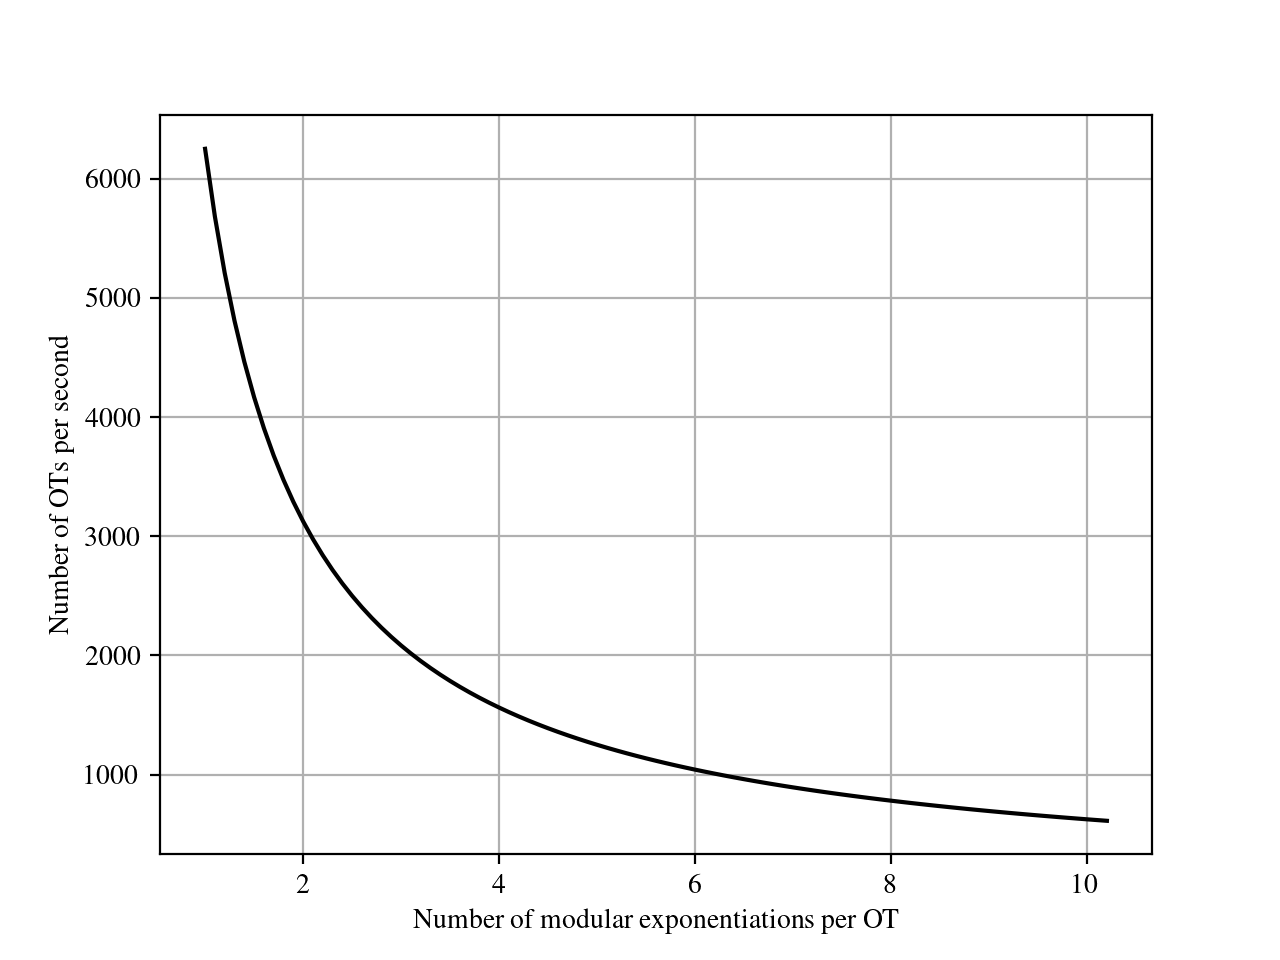
\includegraphics[width=1\textwidth]{Chapter_QuantumAndClassicalObliviousTransfer/nOTperSeccond.png}
\caption{Plot of expression (\ref{eq:nOTs}) on the overestimation of OT rate against the number of modular exponentiation operations required per OT.}
\label{fig:nOTsplot}
\end{figure}
This, however, is a loose overestimation of the number of OTs per second, as it only takes into account the computational complexity of modular exponentiation and assumes that other operations have minimal impact on computation time. Therefore, the actual OT rate must be lower.

For comparison, a study in \cite{ALSZ13} reported that it takes around $18$ ms to generate a Naor-Pinkas OT \cite{NP01} which requires $5$ modular exponentiations, yielding a rate of $56$ OTs per second. These OT rates pose a serious challenge for SMC protocols that rely on OT, such as the Yao SMC protocol \cite{Yao82}. The Yao protocol uses boolean circuits to compute a desired functionality privately and requires half the number of input wires as the number of required OTs. Using the rough OT rate estimation, the OT phase of the Yao protocol with a $32,000$ input boolean circuit would take at least $16$ seconds, and around $2$ minutes and $23$ seconds using Naor-Pinkas OT rate. These execution times can become impractical in deployment environments that require several rounds of circuit evaluation and require higher OT rates.



\subsection{OT extension protocols} \label{Ext-OT}

To improve the efficiency of OT, one potential solution is to replace the computation-intensive asymmetric cryptography with more efficient symmetric cryptography. Symmetric cryptography has the advantage of being faster than asymmetric cryptography. In addition, all known quantum attacks to symmetric cryptography based on the Grover's algorithm only provide a quadratic advantage over classical approaches, which can be mitigated by doubling the size of the symmetric keys \cite{Bernstein2017}. However, despite its efficiency, symmetric cryptography is not enough for OT because it does not meet the asymmetric cryptographic assumptions required by Impagliazzo and Rudich's result \cite{IR99}. Hence, OT cannot be performed solely with symmetric cryptography methods.

To overcome the limitations imposed by Impagliazzo and Rudich's result \cite{IR99} on the use of solely symmetric cryptography for OT, researchers have developed hybrid protocols that combine both symmetric and asymmetric cryptography. Beaver \cite{B96} introduced the idea of extending the number of OTs by using symmetric cryptography, once a small number of base OTs are established using asymmetric cryptography. Although Beaver's original protocol was inefficient, it paved the way for more efficient implementations \cite{IKNP03, N07, NNOB12, ALSZ13, ALSZ15}. Currently, one of the most efficient protocols can generate about $10$ million OTs in $2.62$ seconds \cite{ALSZ13}. The security of these protocols mainly relies on the security of the base OT protocol and the use of quantum secure symmetric tools. However, it's important to note that the protocol analysed in Section~\ref{Ext-OT_comp} \cite{ALSZ13} is not secure against malicious parties and should only be used in a semi-honest environment. To ensure security against malicious parties, extra consistency check phases are necessary, increasing the complexity of the protocol \cite{ALSZ15, KOS15}, as discussed in Section~\ref{Mal-Ext-OT_comp}.



\section{Oblivious transfer complexity analysis} \label{HQOT_comp}

In this section, we compare the complexity of the transfer phase of an optimized version of the BBCS-based QOT protocols ($\Pi^{\textbf{BBCS}}_{\mathcal{F}_{\textbf{COM}}}$ and $\Pi^{\textbf{BBCS}}_{\textbf{bqs}}$) presented before and several well known classical protocols. We start by explaining the optimized version..

\subsection{Optimization}\label{O-OT}

Recall that both $\Pi^{\textbf{BBCS}}_{\mathcal{F}_{\textbf{COM}}}$ and $\Pi^{\textbf{BBCS}}_{\textbf{bqs}}$ can be divided into two phases: the oblivious key distribution phase (we also call it a \textit{precomputation} phase) and the transfer phase. It is interesting to note that both protocols follow the same steps in the transfer phase. We present the transfer phase of both protocols in Figure~\ref{fig:BBCS_Transfer}. We slightly rewrite the protocol by using only one hash function ($H$ describes a random oracle) instead of two random hash functions $f_0$ and $f_1$. This is done for comparison purposes and because, in practice, $H$ is implemented as a specific hash function, such as SHA.

\begin{figure}[h!]
    \centering
        \begin{tcolorbox}[enhanced, 
                        frame hidden,
                        ]
            
            \centerline{$\Pi^{\textbf{BBCS}}$ \textbf{protocol}}
            
            \
            
            \textbf{Alice's input:} $(m_0, m_1)\in\{0,1\}^l$ (two messages). 
            
            \textbf{Bob's input:} $b\in\{0,1\}$ (bit choice).
            
            \
            

            
            \textit{Precomputation phase}: \textcolor{gray}{Alice and Bob generate an oblivious key $(\mathsf{ok}^{\mathsf{A}}, (\mathsf{ok}^{\mathsf{B}}, \mathsf{e}^{\mathsf{B}}))$ according to the corresponding procedure. $\Pi^{\textbf{BBCS}}_{\mathcal{F}_{\textbf{COM}}}$ as in Figure~\ref{fig:BBCS_COM} and $\Pi^{\textbf{BBCS}}_{\textbf{bqs}}$ as in Figure~\ref{fig:BBCS_Bounded}.}
            
            \
            
            \textit{Transfer phase}:
            \begin{enumerate}
            \setcounter{enumi}{4}
                \item Bob defines $I_0 = \{ i : \mathsf{e}^{\mathsf{B}}_i = 0 \}$ and $I_1 = \{ i : \mathsf{e}^{\mathsf{B}}_i = 1 \}$ and sends the pair $(I_b, I_{b\oplus 1})$ to Alice.
                \item Alice computes the pair of strings $(s_0, s_1)$ as $s_i = m_i \oplus H(\mathsf{ok}^{\mathsf{A}}_{I_{b\oplus i}})$ and sends to Bob.
                \item Bob computes $m_b = s_b \oplus  H(\mathsf{ok}^{\mathsf{B}}_{I_0})$. 
            \end{enumerate}
            
            \
            
        \textbf{Alice's output:} $\bot$.
        
        \textbf{Bob's output:} $m_b$.
        
        \end{tcolorbox}
    \caption{Transfer phase of BBCS-based QOT protocols in the $\mathcal{F}_{\mathbf{COM}}-$hybrid model and bounded-quantum-storage model.}
    \label{fig:BBCS_Transfer}
\end{figure}

In the first communication round of the protocol in Figure~\ref{fig:BBCS_Transfer}, Bob sends two sets $(I_b, I_{b\oplus 1})$ to Alice (Step 5). This can be optimized by only sending one set $(I_b)$, as Alice can determine its complement ($\overline{I_b} = I_{b\oplus 1}$) with just one set. This leads to the optimized protocol ($\Pi^{\textbf{BBCS}}_{\textbf{O}}$) shown in Figure~\ref{fig:BBCS_Transfer-optimized}. This optimization results in lower bandwidth requirements compared to the original transfer phase.

The size of the sets can be identified by a symmetric security parameter $\kappa$, as they define the keys ($\mathsf{ok}_{I_i}$, $i=0,1$) used in the hash function $H$. For comparison, we consider $\kappa = 128$. Also, the messages $m_0$ and $m_1$ can be viewed as garbled circuit keys, with a size of $l = 128, 192$ or $256$. If we assume $l \sim \kappa$, the same number of bits are required. This means that in Step 5, Bob only needs to send $l$ bits to Alice, resulting in a reduction of one fourth in the number of bits sent during the transfer phase.

\begin{figure}[h!]
    \centering
        \begin{tcolorbox}[enhanced, 
                        frame hidden,
                        ]
            
            \centerline{$\Pi^{\textbf{BBCS}}_{\textbf{O}}$ \textbf{protocol}}
            
            \
            
            \textbf{Alice's input:} $(m_0, m_1)\in\{0,1\}^l$ (two messages). 
            
            \textbf{Bob's input:} $b\in\{0,1\}$ (bit choice).
            
            \
            

            
            \textit{Precomputation phase}: \textcolor{gray}{Alice and Bob generate an oblivious key $(\mathsf{ok}^{\mathsf{A}}, (\mathsf{ok}^{\mathsf{B}}, \mathsf{e}^{\mathsf{B}}))$ according to the corresponding procedure. $\Pi^{\textbf{BBCS}}_{\mathcal{F}_{\textbf{COM}}}$ as in Figure~\ref{fig:BBCS_COM} and $\Pi^{\textbf{BBCS}}_{\textbf{bqs}}$ as in Figure~\ref{fig:BBCS_Bounded}.}
            
            \
            
            \textit{Transfer phase}:
            \begin{enumerate}
            \setcounter{enumi}{4}
                \item Bob defines $I_0 = \{ i : \mathsf{e}^{\mathsf{B}}_i = 0 \}$ and $I_1 = \{ i : \mathsf{e}^{\mathsf{B}}_i = 1 \}$ and \textbf{sends only} $I_b$ to Alice.
                \item Alice computes the pair of strings $(s_0, s_1)$ as $s_i = m_i \oplus H(\mathsf{ok}^{\mathsf{A}}_{I_{b\oplus i}})$ and sends to Bob.
                \item Bob computes $m_b = s_b \oplus  H(\mathsf{ok}^{\mathsf{B}}_{I_0})$. 
            \end{enumerate}
            
            \
            
        \textbf{Alice's output:} $\bot$.
        
        \textbf{Bob's output:} $m_b$.
        
        \end{tcolorbox}
    \caption{Transfer phase of BBCS-based QOT protocols in the $\mathcal{F}_{\mathbf{COM}}-$hybrid model and bounded-quantum-storage model.}
    \label{fig:BBCS_Transfer-optimized}
\end{figure}


%%%% chatGPT

To fairly compare the transfer phase of the $\Pi^{\textbf{BBCS}}_{\textbf{O}}$ protocol with other classical protocols, we divide classical protocols into precomputation and transfer phases. All steps that are independent of the messages ($m_0$ and $m_1$) and the bit choice ($b$) are considered part of the precomputation phase, while others are included in the transfer phase. The transfer phase is more important to optimize as it is executed during the Yao GC protocol, while the precomputation phase can be performed beforehand.

We stress we will only compare the complexity of different protocols' transfer phase because their precomputation phase rely on different technologies. Since quantum technologies are still in their infancy and constantly evolving, it is difficult to compare the efficiency with classical approaches. However, the oblivious key phase of the $\Pi^{\textbf{BBCS}}_{\textbf{O}}$ protocol has a linear time complexity in all its security parameters, as shown by Lemus et al. \cite{Lemus20}. The time complexity of $\Pi^{\textbf{BBCS}}_{\mathcal{F}_{\textbf{COM}}}$ is $\mathcal{O}(\kappa(2l + t))$, where $\kappa$ is the security parameter of the hash-based commitments, $2l$ is the number of qubits used to generate the oblivious keys, and $t$ is the number of testing qubits.

\subsection{Classical OT} \label{C-OT_comp}

In section \ref{Classical-OT}, we divided the well known Bellare-Micali protocol in these two phases and we observed that it uses three exponentiations during the transfer phase. In Table~\ref{table:ClassicalOT_comparison}, we present the number of required modular exponentiations and communication rounds during the transfer phase of four well known classical protocols that have their security based on the computational hardness of the Discrete Logarithm problem. 

\begin{table}[h!]
\centering
\begin{tabular}{lcc}
\toprule
Protocol & Exponentiation & Comm. rounds \\
\midrule
EGL \cite{EGL85}      & $3$              & $2$\\ 
BM  \cite{BM89}     & $3$              & $2$ \\ 
NP  \cite{NP01}     & $2$             & $2$  \\ 
SimpleOT \cite{CO15} & $1$              & $2$           \\
\bottomrule
\end{tabular}
\caption{Number of modular exponentiation operations and communication rounds executed during the transfer phase of four classical protocols.}
\label{table:ClassicalOT_comparison}
\end{table}

From Table~\ref{table:ClassicalOT_comparison}, we see that the most efficient protocol (SimpleOT \cite{CO15}) still requires one exponentiation operation and $2$ communication rounds. From the above formula (\ref{eq:nOTs}) and setting $C_{mcyles} = 2.5 \times 10^9$, $C_{mexp} = 400\,000$ and $N_{mexp} = 1$, we get an overestimation of around $6 000$ OT per second. Comparing with the rate achieved by OT extension protocols ($10$ million OT in $2.62$ s), it is still very inefficient.

This means current classical OT protocols have a computational complexity limited by $\mathcal{O}(n^{2.58})$ bit operations due to modular exponentiation. The $\Pi^{\textbf{BBCS}}_{\textbf{O}}$ protocol only depends on simple bit operations (XOR, truncation and comparison), meaning its computational complexity is linear in the length of the messages $\mathcal{O}(n)$.

Despite their security guarantees, none of the classical OT protocols discussed are secure against quantum computer attacks. To achieve this level of security, post-quantum approaches must be adopted, which may result in higher computational demands \cite{PST19}. For example, the use of Kyber key encapsulation based on the module learning with errors (M-LWE) problem \cite{CrystalKyber17} in a LAN network results in a rate of only 41 OT per second (24 ms per OT), as reported in \cite{MR19}. This rate is even lower than the rate of 56 OT per second achieved by the Naor-Pinkas protocol \cite{NP01} reported in \cite{ALSZ13}. The NTRU post-quantum encryption system \cite{NTRU} was used in \cite{NTRUOT1, NTRUOT2} to develop a 1-out-of-$n$ OT, which was compared with the SimpleOT protocol \cite{CO15}. Although the individual sides are more efficient in NTRU OT, the overall protocol is still less efficient, with a rate of 728 OT per second ($1.372$ ms per OT) for the highest security level compared to 1375 OT per second ($0.727$ ms per OT) using SimpleOT. It is important to note that these protocols are still vulnerable to \textit{intercept now, decipher later} attacks as they rely on computational assumptions that are only believed to be secure against quantum computer attacks and not proven.


\subsection{OT extension} \label{Ext-OT_comp}

As we explained in section \ref{Ext-OT}, several techniques based on an hybrid symmetric-asymmetric approach were developed as a way to increase the OT execution rate. These techniques use a small number $\kappa$ ($=128$) of base OT protocols (e.g. EGL, BM, NP, SimpleOT) and extend this resource to $m$ ($=10\,000\,000$) OT executions, where $ m >> \kappa$. 

Again, to fairly compare $\Pi^{\textbf{BBCS}}_{\textbf{O}}$ with OT extension protocols, we divide them into precomputation and transfer phases. In this section, we compare the communication and computational complexity of $m$ executions of $\Pi^{\textbf{BBCS}}_{\textbf{O}}$ to one execution of an OT extension protocol, as the latter generates a predetermined number ($m$) of OTs. We compare $\Pi^{\textbf{BBCS}}_{\textbf{O}}$ with the semi-honest ALSZ13 protocol and then with the maliciously secure KOS15 protocol.

\subsubsection{ALSZ13 comparison}

\begin{figure}[t]
    \centering
        \begin{tcolorbox}[enhanced, 
                        frame hidden,
                        ]
                        
			\centerline{\textbf{ALSZ13 OT extensions protocol \citep{ALSZ13}}}
            
			\ 

			\textbf{Alice's input:} $m$ pairs $(x^0_j, x^1_j),\, \forall j\in[m]$ of $l$-bit strings.
            
			\textbf{Bob's input:} $m$ selection bits $\bm{r} = (r_1, ..., r_m)$.

			\
			
			\textit{Initial OT phase (Precomputation phase)}
    \begin{enumerate}
         \item Alice randomly generates a string $\bm{s} = (s_1, ..., s_\kappa)$.
         \item Bob randomly chooses $\kappa$ pairs of $\kappa$-bit strings $\{(\bm{k}^0_i, \bm{k}^1_i)\}^\kappa_{i=1}$.
         \item Bob and Alice execute $\kappa$ base OTs, where Alice plays the role of the receiver with input $\bm{k}$ and Bob plays the role of the sender with messages $(\bm{k}^0_i, \bm{k}^1_i),\, \forall i\in[\kappa]$.
    \end{enumerate}
    \textit{OT extension phase (Transfer phase)}
    \begin{enumerate}
    \setcounter{enumi}{3}
        \item Bob applies a pseudorandom number generator $G$ to $\bm{k}^0_i$, i.e. $\bm{t}^i = G(\bm{k}^0_i)$. Computes $\bm{u}^i = \bm{t}^i \oplus G(\bm{k}^1_i) \oplus \bm{r}$ and sends $\bm{u}^i$ to Alice for every $ i\in[\kappa]$.
        \item Alice computes $\bm{q}^i = (s_i \cdot \bm{u}^i) \oplus G(\bm{k}^{s_i}_i)$.
        \item Alice sends $(y^0_j, y^1_j)$ for every $j\in[m]$, where $y^0_j = x^0_j\oplus H(j,\bm{q}_j)$, $y^1_j = x^1_j\oplus H(j,\bm{q}_j\oplus \bm{s})$ and $\bm{q}_j$ is the $j$-th row of the matrix $Q = [ \bm{q}^1 | ...| \bm{q}^\kappa]$. Note that, in practice, it is required to transpose $Q$ to access its $j$-th row.
        \item Bob computes $x^{r_j}_j = y^{r_j}_j \oplus H(j, \bm{t}_j)$.
    \end{enumerate} 
    
				\textbf{Alice's output:} $\bot$.
    
				\textbf{Bob's output:} $(x^{r_1}_1, ..., x^{r_m}_m)$.

        
        \end{tcolorbox}
    \caption{Precomputation and transfer phases of OT extensions protocol presented in \cite{ALSZ13}.}
    \label{fig:ALSZ13Protocol}
\end{figure}

Let's consider the OT extension protocol proposed in \cite{ALSZ13} (ALSZ13), as illustrated in Figure~\ref{fig:ALSZ13Protocol}. At the time of writing, this protocol reports the fastest implementation with 10 million OTs generated in just 2.68 seconds. The ALSZ13 protocol is divided into two phases: an initial OT phase and an OT extension phase. For comparison purposes, we will focus solely on the second phase, which aligns with our distinction between the precomputation and transfer phases.

In Tables~\ref{table:CvsQ_OT_comparison_computation} and~\ref{table:CvsQ_OT_comparison_communication}, we present a comparison of the computational and communication complexity of the OT extension protocol (ALSZ13) and $\Pi^{\textbf{BBCS}}_{\textbf{O}}$. In Table~\ref{table:CvsQ_OT_comparison_computation}, PRG refers to a pseudorandom generator, $\kappa$ is the number of base OTs executed during the precomputation phase of the OT extension, $m$ represents the total number of OTs, and $l$ is the length of the OT strings. It is assumed that $l \sim \kappa$ have a similar magnitude, as the key length used in the garbled circuits is $l = 128, 192$, or $256$, while $\kappa = 128$ \cite{ALSZ13}. Now, we justify the analysis presented in Tables~\ref{table:CvsQ_OT_comparison_computation} and~\ref{table:CvsQ_OT_comparison_communication}. 

Regarding the ALSZ13 protocol, for every $i\in[\kappa]$, Bob computes two PRGs in step 4 and Alice computes one PRG in step 5. This accounts for $3\kappa$ PRG executions. For every $j \in[m]$, Alice computes two hash functions in step 6 and Bob computes one hash function. This accounts for $3m$ hash functions. For every $i\in[\kappa]$, Bob computes two $m-$bit XOR operations in step 4 and Alice computes one $m-$bit XOR operation. For every $j \in[m]$, Alice computes two $l-$bit XOR operations in step 6 and Bob computes one $l-$bit XOR operation in step 7. Also, for every $j \in[m]$, Alice computes one $\kappa-$bit XOR operation in step 6. This accounts for $3m\kappa + 3ml + m\kappa$ bitwise XOR operations. For every $i\in[\kappa]$, Alice computes one $m-$bit AND operation in step 5. Finally, Alice has to perform a matrix inversion which accounts for around $m\log m$ bit operations. The communication complexity is given by the following elements: Bob sends an $m-$bit vector for every $i\in[\kappa]$ and Alice sends two $l-$bit messages for every $j \in[m]$. This accounts for $2ml + m\kappa$ bits sent.

Regarding the $\Pi^{\textbf{BBCS}}_{\textbf{O}}$ protocol, for every execution of the protocol, Alice computes two hash functions in step 6 and Bob computes one hash function in step 7. This accounts for $3m$ hash functions. Also, Alice computes two $l-$bit XOR operations in step 6 and Bob computes one $l-$bit XOR operation in step 7. This accounts for $3ml$ bitwise XOR operations. For every execution of the protocol, Alice performs $2\kappa$ bitwise comparisons in step 5. Also, Alice computes two $\kappa-$bit truncation in step 6 and Bob computes one $\kappa-$bit truncation in step 7. The communication complexity is given by the following elements: Bob sends a $\kappa-$bit vector and Alice sends two $l-$bit messages, for every execution of the protocol. This accounts for $2ml + m\kappa$ bits sent.

\begin{table}[h!]
\centering
\begin{tabular}{lcc}
\toprule
Operation & ALSZ13 & $\Pi^{\textbf{BBCS}}_{\textbf{O}}$ \\
\midrule
PRG (AES)     & $3\kappa$              & -\\ 
Hash (SHA-1)    & $3m$              & $3m$ \\ 
Bitwise XOR      & $3 m \kappa + 3ml + m\kappa$             & $3ml$  \\ 
Bitwise AND  & $m\kappa$              & -           \\
Matrix transposition & $m\log m$              & -           \\
Bitwise comparison & -             & $2m\kappa$           \\
Bitwise truncation & -            & $3m\kappa$           \\
\bottomrule
\end{tabular}
\caption{Computational complexity comparison between ALSZ13 \cite{ALSZ13} OT extension protocol and $\Pi^{\textbf{BBCS}}_{\textbf{O}}$ protocol from section~\ref{O-OT}.}
\label{table:CvsQ_OT_comparison_computation}
\end{table}

\begin{table}[h!]
\centering
\begin{tabular}{lcc}
\toprule
 & ALSZ13 & $\Pi^{\textbf{BBCS}}_{\textbf{O}}$  \\
\midrule
\multicolumn{1}{l}{Bits sent }   & $2ml  + m\kappa$   & $2ml + m\kappa $  \\
\bottomrule
\end{tabular}
\caption{Communication complexity comparison between ALSZ13 \cite{ALSZ13} OT extension protocol and $\Pi^{\textbf{BBCS}}_{\textbf{O}}$ protocol from section~\ref{O-OT}.}
\label{table:CvsQ_OT_comparison_communication}
\end{table}

The communication complexity is exactly the same in both protocols: $\sim 3ml$. So, the OT extension protocol does not have any advantage over $\Pi^{\textbf{BBCS}}_{\textbf{O}}$ during the communication phase. Regarding their computational complexity, we have to compare the binary operations executed by each protocol.

Firstly, we can see that $\Pi^{\textbf{BBCS}}_{\textbf{O}}$ transfer phase is asymptotically more efficient than ALSZ13 OT extension transfer phase. The computational complexity of OT extension is not linear in the number of OT executions, $\mathcal{O}(m\log m)$, whereas it is linear in the case of $\Pi^{\textbf{BBCS}}_{\textbf{O}}$, $\mathcal{O}(m)$. Now, let us compare the binary operations between each protocol. Denote by $B_{\text{op}}^\text{ALSZ13}$ and $B_{\text{op}}^\text{BBCS}$ the number of binary operations executed by ALSZ13 and $\Pi^{\textbf{BBCS}}_{\textbf{O}}$, respectively. As both protocols execute $3m$ hash functions, we do not take into account their execution. Also, assuming that $\kappa \sim l$, $B_{\text{op}}^\text{ALSZ13}$ is roughly given by,
\begin{eqnarray*}
    B_{\text{op}}^\text{ALSZ13} &=& 3\kappa + 3m\kappa + 3 m l + m\kappa + m\kappa + m \log m \\
    &=& 8 m \kappa + 3 \kappa + m\log m 
\end{eqnarray*}
and $B_{\text{op}}^\text{BBCS} = 8 m \kappa$. Here, we simplify and assume that $3\kappa$ PRGs executions consume only $3\kappa$ bit operations. Therefore, ALSZ13 has more $B_{\text{op}}^\text{ALSZ13} - B_{\text{op}}^\text{BBCS}  \geq m\log m $ binary operations than the transfer phase of $\Pi^{\textbf{BBCS}}_{\textbf{O}}$ protocol. 

%Firstly, we can see that $\Pi^{\textbf{BBCS}}_{\textbf{O}}$ transfer phase is asymptotically more efficient than ALSZ13 OT extension transfer phase. The computational complexity of OT extension is not linear in the number of OT executions, $\mathcal{O}(m\log m)$, whereas it is linear in the case of $\Pi^{\textbf{BBCS}}_{\textbf{O}}$, $\mathcal{O}(m)$. Thus, for a bounded value $l$, $m\log m > ml$ asymptotically. However, in practice, for $l \sim 128$, it would take around $m>10^{50}$ Oblivious Transfers to actually have $m\log m > ml$. Secondly, when comparing $ml$ bit operations with $3m$ SHA$-1$ computations, we conclude that $\Pi^{\textbf{BBCS}}_{\textbf{O}}$ uses less bit operations. Each execution of SHA$-1$ \cite{NISTSHA} requires 80 rounds of several bit operations. If we underestimate the cost of each round and we assume it only requires two bit operations, we get that ALSZ13 OT extension protocol requires at least $3 \times 80\times 2 m = 480 m > ml, \, \forall m$. 

%Let us plot in Fig.~\ref{fig:CvsQ_OT_comparison} the number of bit operations for both protocols. In the case of ALSZ13 OT extension, we underestimate the number of bit operations by considering that SHA$-1$ only costs $480m$ bit operations and that PRG (AES) does not involve any cost. 

%\begin{figure}[!t]
%\centering
%\includegraphics[width=0.5\textwidth]{O-OTVsEXT_OT.png}
%\caption{Bit operation comparison between the transfer phase of O-OT and Extension %OT protocols.}
%\label{fig:CvsQ_OT_comparison}
%\end{figure}

From the results of our comparison, we can conclude that the transfer phase of $\Pi^{\textbf{BBCS}}_{\textbf{O}}$ is competitive with the corresponding phase of the semi-honest ALSZ13 protocol, and has the potential to be even more efficient. Furthermore, the performance of $\Pi^{\textbf{BBCS}}_{\textbf{O}}$ transfer phase is achieved while providing stronger security guarantees. Unlike the ALSZ13 protocol, which relies on computational assumptions of the base OT, $\Pi^{\textbf{BBCS}}_{\textbf{O}}$ has been proven secure against quantum computers. Moreover, while ALSZ13 is a semi-honest protocol (assumes well-behaved parties that follow the protocol), $\Pi^{\textbf{BBCS}}_{\textbf{O}}$ protocol is secure against any corrupted party. To obtain a fair comparison, it is appropriate to consider OT extension protocols that are secure against malicious parties. The work developed in \cite{IKNP03} presented the first protocol in the malicious scenario, which was latter optimised by KOS15 \cite{KOS15} and ALSZ15 \cite{ALSZ15}. Both optimizations carry out one run of the semi-honest OT extension presented in ALSZ13 plus some consistency checks. The protocol presented in \cite{KOS15} adds to ALSZ13 a \textit{check correlation} phase after the transfer phase and the protocol presented in \cite{ALSZ15} adds a \textit{consistency check} phase during the transfer phase. This means that both malicious protocols' transfer phases have greater computational and communication complexity when compared with ALSZ13. Therefore, we can infer that the transfer phase of $\Pi^{\textbf{BBCS}}_{\textbf{O}}$ has lower computational and communication complexity than its malicious classical equivalents. In the next step, we compare the KOS15 protocol \cite{KOS15} with $\Pi^{\textbf{BBCS}}_{\textbf{O}}$.


\subsubsection{KOS15 comparison}\label{Mal-Ext-OT_comp}

KOS15 protocol is very similar to ALSZ13, but it includes an additional phase called \textit{check correlation} phase. This phase ensures that the receiver is well behaved and does not cheat.  In Figure~\ref{fig:K15Protocol}, it is presented the KOS15 protocol that generates $m$ $l$-bit string OT out of $\kappa$ base OT, with computational security given by $\kappa$ and statistical security given by $w$. Note that, in Figure~\ref{fig:K15Protocol}, we join all the subprotocols presented in the original paper: $\prod^{\kappa, m'}_{\textsc{COTe}}$, $\prod^{\kappa, m}_{\textsc{ROT}}$ and $\prod^{\kappa, m}_{\textsc{DeROT}}$. Also, they identify $\mathbb{Z}^\kappa_2$ with the finite field $\mathbb{Z}_{2^\kappa}$ and use $``\cdot"$ for multiplication in $\mathbb{Z}_{2^\kappa}$. For example, the element $\boldsymbol{t}_j$ in $\sum_{j=1}^{m'} \boldsymbol{t}_j \cdot \chi_j$ (Figure~\ref{fig:K15Protocol}, step $10$) should be considered in $\mathbb{Z}_{2^\kappa}$.

\begin{figure}
    \centering
        \begin{tcolorbox}[enhanced, 
                        frame hidden,
                        ]
                        
			\centerline{\textbf{KOS15 OT extensions protocol \citep{KOS15}}}
            
			\ 

    \textbf{Alice's input:} $m$ pairs $(x^0_j, x^1_j),\, \forall j\in[m]$ of $l$-bit strings.
    
    \textbf{Bob's input:} $m$ selection bits $\boldsymbol{r} = (r_1, ..., r_m)$.
    
    \
    
    \textit{Initial OT phase (Precomputation phase)}
    \begin{enumerate}
         \item Alice randomly generates a string $\boldsymbol{s} = (s_1, ..., s_\kappa)$ and Bob randomly chooses $\kappa$ pairs of $\kappa$-bit strings $\{(\boldsymbol{k}^0_i, \boldsymbol{k}^1_i)\}^\kappa_{i=1}$.
         \item Bob and Alice execute $\kappa$ base OTs. Alice plays the role of the receiver with input $\boldsymbol{s}$ and Bob plays the role of the sender with messages $(\boldsymbol{k}^0_i, \boldsymbol{k}^1_i),\, i\in[\kappa]$.
         \item Bob applies a pseudorandom number generator $G$ to $\boldsymbol{k}^0_i$ and $\boldsymbol{k}^1_i$: $\boldsymbol{t}^i = G(\boldsymbol{k}^0_i)$ and $\boldsymbol{t}^i_1 = G(\boldsymbol{k}^1_i)$. Also, set $\boldsymbol{T}^i = \boldsymbol{t}^i \oplus \boldsymbol{t}^i_1$.
         \item Alice applies $G$ to $\boldsymbol{k}^{s_i}_i$ and sets $\boldsymbol{g}^{s_i}_i = G(\boldsymbol{k}^{s_i}_i)$.
    \end{enumerate}
    \textit{OT extension phase (Transfer phase)}
    
    \textit{\hspace{0.25cm} Extend}
    \begin{enumerate}
    \setcounter{enumi}{4}
        \item Bob generates random elements $r_j$, for $r\in [m+1, m']$ and resize $\boldsymbol{r} = (r_1, ..., r_m, r_{m+1}, ..., r_{m'})$, where $m' = m + (\kappa + w)$.
        \item Bob computes $\boldsymbol{u}^i = \boldsymbol{T}^i \oplus \boldsymbol{r}$ and sends $\boldsymbol{u}^i$ to Alice for every $i\in[\kappa]$.
        \item Alice computes $\boldsymbol{q}^i = (s_i \times \boldsymbol{u}^i) \oplus \boldsymbol{g}^{s_i}_i$ for every $i\in[\kappa]$.
    \end{enumerate}
    \textit{\hspace{0.25cm} Check correlation}
    \begin{enumerate}
    \setcounter{enumi}{7}
        \item Sample $(\chi_1, ..., \chi_{m'})\leftarrow \mathcal{F}_{\text{Rand}}(\mathbb{F}^{m'}_{2^\kappa})$.
        \item Bob computes $x = \sum_{j=1}^{m'} r_j \cdot \chi_j$ and $t = \sum_{j=1}^{m'} \boldsymbol{t}_j \cdot \chi_j$, where $\boldsymbol{t}_j$ is the $j$-th row of the matrix $[ \boldsymbol{t}^1 | ...| \boldsymbol{t}^\kappa]$ and sends these to Alice.
        \item Alice computes $q = \sum_{j=1}^{m'} \boldsymbol{q}_j \cdot \chi_j$, where $\boldsymbol{q}_j$ is the $j$-th row of the matrix $Q = [ \boldsymbol{q}^1 | ...| \boldsymbol{q}^\kappa]$, and checks that $t = q + r\cdot \boldsymbol{s}$. If the check fails, output \textsc{Abort}, otherwise continue. %Alice outputs $\Delta$, $\{\boldsymbol{q}_j\}_{j\in[m]}$ and Bob outputs $\{\boldsymbol{t}_j, r_j\}_{j\in [m]}$.
    \end{enumerate} 
    
    \textit{\hspace{0.25cm} Randomize and encrypt}
    \begin{enumerate}
    \setcounter{enumi}{10}
        \item Alice sends $(y^0_j, y^1_j)$ for every $j\in[m]$, where $y^0_j = x^0_j\oplus H(j,\boldsymbol{q}_j)$, $y^1_j = x^1_j\oplus H(j,\boldsymbol{q}_j\oplus \boldsymbol{s})$. % and $\boldsymbol{q}_j$ is the $j$-th row of the matrix $Q = [ \boldsymbol{q}^1 | ...| \boldsymbol{q}^\kappa]$. Note that, in practice, it is required to transpose $Q$ to access its $j$-th row.
        \item Bob computes $x^{r_j}_j = y^{r_j}_j \oplus H(j, \boldsymbol{t}_j)$.
    \end{enumerate} 
    
    \textbf{Alice's output:} $\bot$.
    
    \textbf{Bob's output:} $(x^{r_1}_1, ..., x^{r_m}_m)$.

        
        \end{tcolorbox}
    \caption{Precomputation and transfer phases of OT extensions protocol presented in \cite{KOS15}.}
    \label{fig:K15Protocol}
\end{figure}

\begin{table}
\centering
\begin{tabular}{lcc}
\toprule
Operation & KOS15 & $\Pi^{\textbf{BBCS}}_{\textbf{O}}$ \\
\midrule
Hash (SHA-1)    & $3m$              & $3m$ \\ 
Bitwise XOR      & $3 m\kappa + 3ml + m\kappa$             & $3ml $  \\ 
Bitwise AND  & $m\kappa$              & -           \\ 
Matrix transposition & $m\log m$              & -           \\ 
Bitwise comparison & -             & $2ml$           \\ 
Bitwise truncation & -            & $3ml$           \\ 
$\kappa$-bit additon & $3(m + (\kappa + w))\kappa$ & - \\ 
$\kappa$-bit mult & $2(m + (\kappa + w))\kappa^{1.58}$ & - \\ 
\bottomrule
\end{tabular}
\caption{Computational complexity comparison between KOS15 \cite{KOS15} OT extension protocol and $\Pi^{\textbf{BBCS}}_{\textbf{O}}$ protocol from section~\ref{O-OT}.}
\label{table:complexity}
\end{table}

\begin{table}[h!]
\centering
\begin{tabular}{lcc}
\toprule
 & KOS15 & $\Pi^{\textbf{BBCS}}_{\textbf{O}}$  \\
\midrule
\multicolumn{1}{l}{Bits sent }   & $2ml  + m\kappa + \kappa$   & $2ml + m\kappa $  \\
\bottomrule
\end{tabular}
\caption{Communication complexity comparison between KOS15 \cite{KOS15} OT extension protocol and $\Pi^{\textbf{BBCS}}_{\textbf{O}}$ protocol from section~\ref{O-OT}.}
\label{table:communication}
\end{table}



The KOS15 protocol, like $\Pi^{\textbf{BBCS}}_{\textbf{O}}$ and ALSZ13, begins with a precomputation phase that can be performed prior to the actual OT computation. However, the KOS15 paper \cite{KOS15} originally carried out the computation of PRGs $G$ during the OT extension phase. These $3\kappa$ computations of $G$ can actually be done during the precomputation phase as they are independent of the input elements. The main difference between KOS15 and ALSZ13 lies in steps $9-11$, the check correlation phase. In this phase, both parties utilize a random oracle functionality $\mathcal{F}_{\text{Rand}}(\mathbb{F}^{m'}_{2^\kappa})$ to obtain equal random values. Bob then performs twice $m'$ $\kappa$-bit sums, $m'$ $\kappa$-bit multiplications and sends $2\kappa$ bits ($x$ and $t$) to Alice, who in turn performs $m'$ $\kappa$-bit sums and $m'$ $\kappa$-bit multiplications. For the purpose of simplicity, we assume that each $\kappa$-bit sum takes $\kappa$ bit operations, and multiplication takes $\kappa^{1.585}$, using the Karatsuba method for multiplication with $O(\kappa^{1.585})$ complexity and schoolbook addition with $O(\kappa)$ complexity.

Let us compare the binary operations between KOS15 and $\Pi^{\textbf{BBCS}}_{\textbf{O}}$ as we did with the ALSZ13 protocol. Denote by $B_{\text{op}}^\text{KOS15}$ and $B_{\text{op}}^\text{BBCS}$ the number of binary operations executed by KOS15 and $\Pi^{\textbf{BBCS}}_{\textbf{O}}$, respectively. Again, without taking into account the execution of $3 m$ hash functions and assuming that $\kappa \sim l$, $B_{\text{op}}^\text{KOS15}$ is roughly given by,
\begin{eqnarray*}
\begin{split}
    B_{\text{op}}^\text{KOS15} &= 3m\kappa + 3ml + m\kappa \\
    &+ m\kappa + m \log m \\
    &+ 3(m + (\kappa + w))\kappa \\
    &+ 2(m + (\kappa + w))\kappa^{1.58}\\
    &= 11 m \kappa  + m\log m \\
    &+ 3\kappa^2 + 3w\kappa  \\
    &+ 2 m \kappa^{1.58} + 2 \kappa^{2.58} + 2w\kappa^{1.58}
\end{split}
\end{eqnarray*}
and $B_{\text{op}}^\text{BBCS} = 8 m \kappa$. Therefore, KOS15 has more $B_{\text{op}}^\text{KOS15} - B_{\text{op}}^\text{BBCS}  \geq 5 m\kappa + m\log m$ binary operations than $\Pi^{\textbf{BBCS}}_{\textbf{O}}$ transfer phase. 
%Now, since $m$ SHA-1 executions requires at least $480 m$ binary operations \cite{Santos2021, NISTSHA} and a common value for $\kappa$ is $\kappa = 128$ \cite{K15}, we have that $m$ SHA-1 executions requires at least $3 m \kappa$ binary operations. Adding $3 m \kappa$ to $4 m\kappa$, we have that KOS15 has at least $7 m\kappa$ more binary operations than HQOT transfer phase, which is almost twice as much binary operations as the quantum version ($\sim 88\%$). 
For this estimation, note that we are considering the lower bound $2 m \kappa$ instead of $2 m \kappa^{1.58}$ and we are not taking into account the implementation of the random oracle $\mathcal{F}_{\text{Rand}}(\mathbb{F}^{m'}_{2^\kappa})$, which would add an extra cost linear in the number of OT executions.

Regarding the communication complexity, the number of bits sent during both KOS15 and $\Pi^{\textbf{BBCS}}_{\textbf{O}}$ is almost the same. KOS15 only adds $\kappa$ bits to the communication during the check correlation phase. However, since this overhead is independent of $m$ (number of OTs executed) its effect is amortized for big $m$.

\section{Conclusion}


The security and efficiency of OT implementations is crucial for secure computations, especially in the context of Yao's garbled circuit protocol. While classical OT protocols rely on asymmetric cryptographic primitives, which are known to be vulnerable to quantum attacks or have security based on conjectures, several works \cite{Lemus20, BCKM21, GLSV21, U10} have used the laws of physics to prove the security of BBCS-based QOT protocols against malicious adversaries with access to quantum computers. Additionally, using oblivious keys can separate the quantum technological burden from the execution of OT and enable efficient implementation.

In this chapter, we compared the transfer phase of an optimized version ($\Pi^{\textbf{BBCS}}_{\textbf{O}}$) of the BBCS-based QOT protocol with the transfer phase of the currently fastest implementation of OT (ALSZ13). Our results showed that the transfer phase of $\Pi^{\textbf{BBCS}}_{\textbf{O}}$ has the potential to be faster than the ALSZ13 protocol while offering higher security. In addition to being secure against quantum computer attacks, BBCS-based QOT protocols are also secure in the malicious setting, whereas ALSZ13 is only secure in the semi-honest model. Furthermore, our analysis revealed that the transfer phases of current maliciously secure implementations (ALSZ15 and KOS15) have a higher computation and communication complexity than $\Pi^{\textbf{BBCS}}_{\textbf{O}}$. In the next chapter, we compare the performance of a secure multiparty computation system based on both classical OT and BBCS-based QOT protocols. 

%\bibliography{bibforthesis}
%\bibliographystyle{unsrt}
%\end{document}

%%\documentclass[11pt]{report}



%\begin{document}

\chapter{Quantum oblivious linear evaluation}
\label{ch:QOLE}

Oblivious Linear Evaluation (OLE) is a cryptographic task that permits two distrustful parties, say Alice and Bob, to jointly compute the output of a linear function $f(x)=ax+b$ in some finite field, $\mathbb{F}$. Alice provides inputs $a, b\in\mathbb{F}$ and Bob provides $x\in\mathbb{F}$, while the output, $f(x)$, becomes available only to Bob. As the parties are distrustful, a secure OLE protocol should not permit Alice to learn anything about Bob's input, while also Alice's inputs should remain unknown to Bob.  OLE can be seen as a generalization of oblivious transfer (OT) \cite{Rabin81}, a basic primitive for secure two-party computation, which is a special case of secure multi-party computation \cite{Goldreichbook04,CCD88,Canetti00MPC}. OT has been shown to be complete  for secure multi-party computation, i.e., any such task, including OLE, can be achieved given an OT implementation. 
 
Impagliazzo and Rudich proved that OT protocols require public-key cryptography and cannot just rely on symmetric cryptography \cite{IR89}. Consequently, OLE cannot rely on symmetric cryptography either, and we need to resort to public-key cryptography.  However, Shor's  quantum algorithm \cite{Sho95}  poses a threat to the currently deployed public-key systems, motivating the search for protocols secure against quantum attacks. Bennet et al. \cite{BBCS92} and Cr{\'e}peau \cite{C94} proposed the first protocols for quantum OT (QOT). As far as quantum OLE (QOLE) is concerned, to the best of our knowledge, no protocol has been proposed as of now.
Analogously to the classical case, it is expected that one can implement QOLE based on QOT protocols. That said, in this work we propose a protocol for QOLE that, additionally, does not rely on any QOT implementation.

OLE is commonly generalised to vector OLE (VOLE). In this setting, Alice defines a set of $k$ linear functions $(\bm{a}, \bm{b})\in\mathbb{F}^k\times\mathbb{F}^k$ and Bob receives the evaluation of all these functions on a specified element $x\in\mathbb{F}$, i.e. $\bm{f}:=\bm{a} x+ \bm{b}$. One can think of VOLE as the arithmetic analog of string OT and show how it can be used  in certain Secure Arithmetic Computation and Non-Interactive Zero Knowledge proofs \cite{BCGI18}. Ghosh et. al  put further in evidence the usefulness of VOLE by showing that it serves as the building block of Oblivious Polynomial Evaluation \cite{GNN17}, a primitive which allows more sophisticated applications, such as password authentication, secure  list intersection,  anonymous complaint boxes \cite{NP06}, anonymous initialization for secure metering of client visits in servers \cite{NP99},  secure Taylor approximation of relevant functions (e.g. logarithm) \cite{LP02}, secure set intersection \cite{H18} and distributed generation of RSA keys \cite{G99}.  We also show how our QOLE protocol can be adapted to achieve secure VOLE.

\section{Contributions overview}\label{Intro_contributions}

We present a quantum protocol for OLE with universally composable security (quantum-UC security, see Definition \ref{def:statisticalquc}) in the $\mathcal{F}_{\textbf{COM}}-$hybrid model, i.e. when assuming the existence of a commitment functionality, $\mathcal{F}_{\textbf{COM}}$ (see Figure \ref{fig:func_com}). To obtain a secure protocol, we take advantage of the properties of mutually unbiased bases (MUBs) in high-dimensional Hilbert spaces with prime and prime-power dimension. Such a choice is motivated by recent theoretical and experimental advances that pave the way for the development and realization of new solutions for quantum cryptography \cite{BPT00, CBKG02, AGS03, AKBH07, SS10, DEBZ10, Zhongetal2015, Sitetal17, Bouchardetal18, BHVBFHM18, DHMPPV21}. To the best of our knowledge, our protocol is the first proposal of a QOLE protocol proved to be quantum-UC secure. Moreover, it is not based on any QOT implementation which would be the standard approach. To prove its security, the only assumption we make is the existence of a commitment functionality. We consider the static corruption adversarial model with both semi-honest and dishonest adversaries. Finally, we modify the proposed protocol to generate quantum-UC secure VOLE.

\

\noindent\textbf{Main tool.} The proposed protocol $\Pi_{\textbf{QOLE}}$ (see Figure \ref{fig:fullprotocol}) is based on the fact that in a Hilbert space of dimension $d$ (isomorphic to $\mathbb{Z}_d$) there exists a set of MUBs $\{\ket{e^x_r}\}_{x, r\in\mathbb{Z}_d}$, such that, upon the action of a certain operator $V^b_a$,  each basis element $r$ is shifted by some linear factor $ax - b$ inside the same basis $x$:

\begin{equation}
    V^b_a \ket{e^x_r} = c_{a,b,x, r} \ket{e^x_{ax - b + r}},
    \label{eq:main_equation_1.3.}
\end{equation}
where $a, b, x, r \in \mathbb{Z}_d =\{0,1,\ldots,d-1\}$. If Alice controls the operator $V^b_a$ and Bob controls the quantum state $\ket{e^x_r}$, they are able to compute a linear function $f(x) = ax - b$ where effectively Alice controls the function $f = (a, b)$ and Bob controls its input $x$. Moreover, since Bob controls $x$ and $r$, he can receive $f(x)$ by measuring the output element. 

\

\noindent\textbf{Protocol overview.} In a nutshell, the QOLE protocol (see Figure \ref{fig:fullprotocol}) with inputs $f = (a,b)$ from Alice and $x$ from Bob is divided into two main phases. In the first \textit{quantum phase}, Alice and Bob use high-dimensional quantum states to generate $n$ random weak OLE (RWOLE) instances, where $n$ is the security parameter.  In this phase, Alice  outputs  $n$ random elements $f^0_i = (a^0_i, b^0_i)$, and Bob  outputs $n$ elements $(x^0_i, y^0 = f^0_i(x^0_i))$. These instances are considered to be weaker because Bob is allowed to have some amount of information about the $n$ outputs of Alice $(a^0_i, b^0_i)$. In the second \textit{post-processing phase}, Alice and Bob use classical tools to extract one secure OLE from the aforementioned $n$ instances.

More specifically, in the quantum phase, Bob randomly generates $m=(1 + t)n$ quantum states $\ket{e^{x^0_i}_{r_i}}$ and sends them to Alice. Then, Bob commits to his choice $(x^0_i, r_i)$, $\forall i\in [m]$, where for any $l\in\mathbb{N}$, $[l]$ denotes the set $\{1, \ldots, l\}$, using an ideal commitment functionality, $\mathcal{F}_{\textbf{COM}}$, and Alice asks to verify  a subset $T$ of size $tn$ of these commitments. This intermediate \textit{commit-and-open} step allows Alice to test Bob's behaviour and ensure that he does not deviate \textit{too much} from the protocol, and it is a common method used in security proofs of QOT protocols \cite{Unruh10, DFLSS09}. If Bob passes all the tests, Alice randomly generates $(a^0_i, b^0_i)$ and applies $V^{b^0_i}_{a^0_i}$ to the remaining $n$ received states $\ket{e^{x^0_i}_{r_i}}$,  for $i\in [m]\setminus T$.  For the rest of this section we relabel and denote $[n]=[m]\setminus T$. According to the expression~\eqref{eq:main_equation_1.3.}, the output states are given by $\ket{e^{x^0_i}_{a^0_i x^0_i - b^0_i + r_i}}$ and she sends them to Bob, who outputs $y^0_i = a^0_i x^0_i - b^0_i$ by measuring the received states in the corresponding basis $ x^0_i$ and subtracting $r_i$,  $\forall i\in [n]$. 

The post-processing phase uses two subprotocols: a derandomization step (see Figure \ref{fig:nOLE}) and an extraction step (see Figure \ref{fig:privacy_amplification}). The derandomization step is based on the protocol $\Pi^n_{\text{OLE}}$ from \cite{DHNO19} and transforms the $n$ RWOLE instances into $n$ weak OLE (WOLE) instances with inputs $(a_i, b_i)_{i\in [n]}$ chosen by Alice and inputs $x_i$ for $i\in [n]$ chosen by Bob. The extraction protocol uses the so-called \textit{Multi-linear Modular Hashing} family, MMH$^*$, of two-universal hash functions \cite{HK97} to render Bob's information on Alice's system useless and to extract one secure OLE out of $n$ instances of WOLE. In the extraction phase, Alice samples a two-universal hash function $g_{\bm{\kappa}}$ from MMH$^*$ and sends it to Bob. Then, with adequately-crafted vectors $(\bm{a}, \bm{b}) = \big( (a_1, \ldots, a_n), (b_1, \ldots, b_n) \big)$, Alice has $a = g_{\bm{\kappa}}(\bm{a})$ and $b = g_{\bm{\kappa}}(\bm{b})$, and Bob outputs $y = g_{\bm{\kappa}}(\bm{y})$, where $\bm{y} = \bm{a} \bm{x} + \bm{b}$ after point-wise vector multiplication with the constant vector $\bm{x} = (x, \ldots, x)$. 



\


\noindent\textbf{quantum-UC security.} %The intuition behind the security of the proposed protocol $\Pi_{\textbf{QOLE}}$ comes from the following observations. 
Due to the quantum nature of the states $\ket{e^{x^0_i}_{r_i}}_{i\in [n]}$, a dishonest Alice is not able to distinguish which bases $x^0_i, i\in [n]$ are used by Bob. From her point of view, Bob's states are maximally mixed and therefore completely hide $x^0_i$. This is enough to ensure that, in the derandomization step, Alice does not receive any information about Bob's final input $x$. For a dishonest Bob, to correctly pass all Alice's tests, it means he did not cheat at all rounds with overwhelming probability. This ensures that he  has some \textit{bounded} information on Alice's random elements $(a^0_i, b^0_i)_{i\in [n]}$, and using privacy amplification techniques in the extraction step, Alice can guarantee that Bob's information about her final input $(a,b)$ is the same as in the case of an ideal OLE functionality, i.e. the probability distribution of $a$ is close to uniform.

Turning this intuition into a quantum-UC security proof requires some additional insights. First, we need a way to quantify Bob's information on Alice's elements $(a^0_i, b^0_i)$ after the testing phase and the application of the corresponding $V^{b^0_i}_{a^0_i}$  operators, for $ i\in [n]$; for this purpose we use the quantum \textit{min-entropy} (see Definition \ref{def:conditionalquantumminentropy}). We follow the approach of \cite{DFLSS09} to guarantee that Bob does not significantly deviate from the protocol in all the rounds, and we use Theorem 1 from~\cite{Dupuis2015} to compute a concrete lower bound of Bob's min-entropy on Alice elements $(a^0_i, b^0_i)_{i\in [n]}$. Along with Lemma \ref{lem:leftover}, we have that $a = g_{\bm{\kappa}}(\bm{a})$ is close to uniform, which is sufficient to prove that Bob does not know more about $(a,b)$ than what the output $y = ax + b$ reveals. 

In order to show that the protocol $\Pi_{\textbf{QOLE}}$ is quantum-UC secure, we need to show that an ideal execution of $\Pi_{\textbf{QOLE}}$ with access to $\mathcal{F}_{\textbf{OLE}}$ (Figure \ref{fig:OLE_functionality}) is indistinguishable from a real execution of the protocol from the point of view of an external entity called the \textit{environment}. To prove this indistinguishability, we have to build a simulator that simulates the execution of the protocol in the ideal setting and generates messages on behalf of the honest simulated parties,  while trying to extract the dishonest party's inputs and feed them in $\mathcal{F}_{\textbf{OLE}}$. In particular, for a dishonest Alice, we have to demonstrate the existence of a simulator, $\mathcal{S}_A$, that generates messages on behalf of honest Bob and extracts Alice's input $(a,b)$ which, in turn, feeds into $\mathcal{F}_{\textbf{OLE}}$.  To this end, we consider that $\mathcal{S}_A$ simulates an attack by Bob at all rounds, $i$, of the protocol  which allows to extract the $m$ values of Alice  $(a^0_i,b^0_i)$. However, the commit-and-open scheme described above is designed to catch such an attack, and to work around this issue we substitute the ideal commitment functionality, $\mathcal{F}_{\textbf{COM}}$, with a fake commitment functionality, $\mathcal{F}_{\textbf{FakeCOM}}$, that allows $\mathcal{S}_A$ to open the commitments later \cite{Unruh10}.  From the remaining $n$ values $(a^0_i,b^0_i)$, $\mathcal{S}_A$ computes Alice's input $(a,b)$ and feeds it to $\mathcal{F}_{\textbf{OLE}}$.

For a dishonest Bob, we have to show the existence of a simulator, $\mathcal{S}_B$, that generates messages on behalf of  honest Alice and extracts Bob's input $x$. We assume that $\mathcal{S}_B$ has full control over  $\mathcal{F}_{\textbf{COM}}$, which means that it has access to Bob's $m$ committed values $(x^0_i, r_i)$;  the input $x$ can be easily extracted from these values. %The rest of the simulation goes according to the output value of the ideal OLE functionality $y$ on the simulator input $x$. {\cv not sure what the last sentence means}

\

\noindent\textbf{Protocol generalization.}  We start by generalizing   the main relation (\ref{eq:main_ingredient}) to Galois Fields of prime-power dimension, $GF(d^M) \text{ for }M>1$. Then, we show how we can obtain a protocol for quantum VOLE. In particular, from $n$ WOLE instances, we are able to generate a VOLE with size proportional to $n$, and we  bound this proportion by the min-entropy value on the WOLE instances.


\subsection{Organization}\label{Intro_organization}
In Section \ref{Prelim_MUB}, we introduce the main tool used in the QOLE protocol. In Section \ref{insecureQOLE}, in order to build some intuition, we present a QOLE protocol that is secure only if we consider Bob to be semi-honest; in case Bob is dishonest, its security is compromised. In Section \ref{secureQROLE_overview}, we construct a secure protocol that comprises the first part of our main QOLE protocol presented in Section \ref{qole_protocol}. Next, in Section \ref{secureQROLE_protocol}, we prove the security of the QOLE protocol in the quantum-UC framework. Then, in Section \ref{sec:protgeneral}, we show how to generalise the presented QOLE protocol to  Galois Fields of prime-power dimensions and we also present a quantum-UC secure protocol achieving VOLE.


\section{Mutually unbiased bases}\label{Prelim_MUB}

In this section, we present the basics and some properties of mutually unbiased bases (MUBs) in some high-dimensional Hilbert space $\mathcal{H}^d$. This is the main tool that is used in our protocol. For more details about MUBs see \cite{DEBZ10}.

\begin{definition}
Let $\mathcal{B}_0 = \{\ket{\psi_1}, \ldots, \ket{\psi_d}\}$ and $\mathcal{B}_1 = \{\ket{\phi_1}, \ldots, \ket{\phi_d}\}$ be orthonormal bases in the d-dimensional Hilbert space $\mathcal{H}^d$. They are said to be \textit{mutually unbiased} if $| \braket{\psi_i}{\phi_j} | = \frac{1}{\sqrt{d}}$ for all $i, j\in \{1,\ldots,d\}$. Furthermore, a set $\{\mathcal{B}_0, \ldots, \mathcal{B}_m\}$ of orthonormal bases on $\mathcal{H}^d$ is said to be a set of MUBs if, for every $i\neq j$, $\mathcal{B}_i$ is mutually unbiased with $\mathcal{B}_j$.
\end{definition}

MUBs are extensively used in quantum cryptography because, in some sense, these bases are as far as possible from each other and the overlap between two elements from different bases is constant. Let $\big\{\ket{0}, \ldots, \ket{d-1}\big\}$ be the computational basis of $\mathcal{H}^d$, where $d$ is a prime number, and $\big\{\ket{\tilde{0}}, \ldots, \ket{\widetilde{d-1}}\big\}$ be the dual basis which is given by the Fourier transform on the computational basis:
\begin{equation*}
    \ket{\tilde{j}} = \frac{1}{\sqrt{d}} \sum_{i=0}^{d-1} \omega^{-i j} \ket{i},\label{eq:dualbasis}
\end{equation*}
where $\omega = e^{\frac{2\Pi i}{d}}$. We can easily verify that the computational basis and its dual basis are mutually unbiased, and we will make use of the following two operators, $V^0_a$ and $V^b_0$, to encode Alice's functions during the first (quantum) phase of the protocol.

\begin{definition}[Shift operators]
The \textit{shift operator} $V^0_a$ shifts the computational basis by $a$ elements, i.e.
\begin{equation*}
    V^0_a\ket{i} = \ket{i+a}.\label{eq:shiftoperato}
\end{equation*}

Similarly, the \textit{dual shift operator} $V^b_0$ shifts the dual basis by $b$ elements, i.e.

\begin{equation*}
    V^b_0\ket{\tilde{j}} = \ket{\widetilde{j-b}}.\label{eq:dualshift}
\end{equation*}
\end{definition}
The operators $V^0_a$ and $V^b_0$ are diagonal in the dual and computational basis, respectively\footnote{Note that $V^0_a$ and $V^b_0$ can be seen as a generalization of the Pauli $X$ and $Z$ operators, respectively.}, i.e.
\begin{equation*}
    V^0_a = \sum_{j=0}^{d-1} \omega^{a j} \ketbra{\tilde{j}}{\tilde{j}} \text{ and }V^b_0 = \sum_{i=0}^{d-1} \omega^{b i} \ketbra{i}{i}.
\end{equation*}
Furthermore, following the convention from \cite{DEBZ10}, we can define
\begin{eqnarray*}
V^b_a &:=& V^b_0 V_a^0= \sum^{d-1}_{l=0} \omega^{(l+a)b} \ketbra{l+a}{l},
\end{eqnarray*}
obtaining the so-called \textit{Heisenberg-Weyl operators}. These operators form a group of unitary transformations with $d^2$ elements; the group has $d+1$ commuting abelian subgroups of $d$ elements, and for each abelian subgroup, there exists a basis of joint eigenstates of all $V^b_a$ in the subgroup. These $d+1$ bases are pairwise mutually unbiased.
Let $x\in\mathbb{Z}_{d+1}$ label the abelian subgroups, let $l\in\mathbb{Z}_d$ label the elements of each subgroup, and let $U^x_l$ denote the corresponding subgroup operators. Finally, let the $i-$th basis element associated with the $x-$th subgroup be denoted by $\ket{e^x_i}$. Then, it can be seen that \cite{DEBZ10},

\begin{equation*}
    U^x_l = \sum^{d-1}_{i=0} \omega^{i l} \ketbra{e^x_i}{e^x_i} \text{ and }\ket{e^x_i} = \frac{1}{\sqrt{d}} \sum^{d-1}_{l=0} \omega^{- i l + \frac{l(l-1)}{2}x}\ket{l},
\end{equation*}
where
\begin{equation*}
    U^x_l = \alpha^x_l V^{x l}_l \text{ with }\alpha^x_l = \omega^{-x l(l+1)/2}.
\end{equation*}
One can show that
\begin{equation*}
  V^b_a \ket{e^x_0} = c_{x,a,b} \ket{e^x_{ax - b}},\, x\in\mathbb{Z}_d  \text{ and }
V^b_a \ket{e^d_0} = c_{d,a,b} \ket{e^d_a} {\text{ for } x=d},\end{equation*}
or more generally
\begin{equation}
    V^b_a \ket{e^x_r} = c_{a, b, x, r} \ket{e^x_{ax - b + r}}, \text{ with }\, c_{a, b, x, r} = \omega^{ar + \frac{a(a+1)}{2}x}. \label{eq:main_relation}
\end{equation}
\begin{proof}
By definition, we have that
\begin{eqnarray*}
V^b_a \ket{e^x_r} &=& \frac{1}{\sqrt{d}} \sum_{k,l = 0}^{d-1} \omega^{(k+a)b}\ketbra{k+a}{k} \omega^{-rl + \frac{l(l-1)}{2}x} \ket{l}\\
&=&  \frac{1}{\sqrt{d}} \sum_{l = 0}^{d-1} \omega^{(l+a)b} \omega^{-rl + \frac{l(l-1)}{2}x} \ket{l+a}\\
&=&  \frac{1}{\sqrt{d}} \sum_{l = 0}^{d-1} \omega^{lb}\omega^{-r(l-a) + \frac{(l-a)(l-a-1)}{2}x} \ket{l} \\
&=&  \frac{\omega^{ar}}{\sqrt{d}} \sum_{l = 0}^{d-1} \omega^{-l(-b+r)}\omega^{ \frac{l(l-1)}{2}x + lax + \frac{a(a+1)}{2}x } \ket{l} \\
&=&  \frac{\omega^{ar}}{\sqrt{d}} \sum_{l = 0}^{d-1} \omega^{-l(-b+r)}\omega^{ \frac{l(l-1)}{2}x - lax + \frac{a(a+1)}{2}x } \ket{l} \\
&=&  \frac{\omega^{ar + \frac{a(a+1)}{2}x}}{\sqrt{d}} \sum_{l = 0}^{d-1} \omega^{-l(ax-b+r) + \frac{l(l-1)}{2}x}\\
&=& \omega^{ar + \frac{a(a+1)}{2}x \ket{e^x_{ax - b + r}}}.
\end{eqnarray*}
\end{proof}
This last property is the main ingredient for the construction of our protocol as it encodes a linear evaluation based on values $a$, $b$ and $x \in \mathbb{Z}_d$\footnote{While $x \in \mathbb{Z}_{d+1}$, henceforth we consider $x \in \mathbb{Z}_{d}$, since we only use $d $ out of the $d+1$ MUBs.}. In our protocol, we take $a,b$ -- that determine the operators $V^b_ a$ -- to be Alice's inputs and $x$ to be Bob's input.

Finally, let us see how the operators $V^b_a$ act on the so-called \textit{generalised Bell states}, since Bob's attack to the protocol is based on that. We start with the definition of the \textit{seed} Bell state 
\begin{equation*}
    \ket{B_{0,0}} = \frac{1}{\sqrt{d}}\sum_{i} \ket{i^*, i},\label{eq:Bellseed}
\end{equation*}
where the map $\ket{\psi}\rightarrow\ket{\psi^*}$ is defined by taking the complex conjugate of the coefficients:

$$\ket{\psi} = \sum_i \beta_i \ket{i}\rightarrow \ket{\psi^*} = \sum_i \beta_i^* \ket{i}.$$

Using the properties of the operators $V_a^b$, we can derive the rest of the generalised Bell states from the seed state, as

\begin{eqnarray}
\ket{B_{a,b}} &=& (\mathds{1} \otimes V^b_a) \ket{B_{0,0}} = \frac{1}{\sqrt{d}} \sum_{i=0}^{d-1} \omega^{(i+a)b} \ket{i^*, i+a}, \label{eq:bob_attack}
\end{eqnarray}
and one can prove that the set $\{\ket{B_{a, b}}\}_{(a,b) \in\mathbb{Z}_d^2}$ constitutes an orthonormal maximally entangled basis in the Hilbert space of two-qudit states \cite{DEBZ10}.



\section{Semi-honest QOLE protocol}\label{insecureQOLE}

 In order to build some intuition on the proposed protocol for QOLE, we start by presenting a simpler protocol that is only secure under the semi-honest adversarial model. This semi-honest version leverages the properties of MUBs explored in Section~\ref{Prelim_MUB} and, in particular, the one presented in expression~\eqref{eq:main_relation}. As we saw, given the set of MUBs $\{ \ket{e^x_r} \}_{r\in\mathbb{Z}_d},\ \forall x\in\mathbb{Z}_d$, the operators $V^b_a$ simply permute the elements inside the basis $x$, according to a linear combination of the elements $a$, $b$, $x$ and $r$:

\begin{equation}
V^b_a \ket{e^x_r} = c_{a, b, x, r} \ket{e^x_{ax - b +r}}.
\label{eq:main_ingredient}
\end{equation}

Alice and Bob can use the above property to compute together a linear function $f(x) = ax - b$, where Alice chooses the parameters $a$ and $b$, and Bob chooses the input element $x$. The protocol summarized in Figure~\ref{fig:SH_QOLE}. Bob starts by choosing a basis $x$ and an element $r$ therein, and prepares the state $\ket{e^x_r}$:  the basis choice $x$ plays the role of the input element $x$, and the basis element $r$ is used to enhance Bob's security against a potentially dishonest Alice. Then, he sends the  state $\ket{e^x_r}$ to Alice, who, in turn, applies on it the operator $V^b_a$ and sends back to Bob the resulting state. According to ~\eqref{eq:main_ingredient}, Bob receives $\ket{e^x_{ax - b + r}}$,  measures it in the $x$ basis, and outputs the linear function evaluation $f(x) = ax-b$ by subtracting $r$. Thus, the correctness of the protocol is ensured by expression~\eqref{eq:main_ingredient}.
%\begin{figure}[!h]
%\centering
%\framebox[\linewidth][l]{%
%    \parbox{0.95\linewidth}{%
%    \begin{center}
%        \textbf{Semi-honest QOLE}
%    \end{center}
%    
%    \textbf{Alice's input:} $(a, b) \in \mathbb{Z}^2_d$
%    
%    \textbf{Bob's input:} $x \in\mathbb{Z}_d$
%    
%    \
%    
%    \begin{enumerate}
%     
%        \item Bob  randomly generates $r \in \mathbb{Z}_d$. He prepares and sends the state $\ket{e^x_r}$ to Alice.
%        \item Alice prepares the operator $V^b_a$ according to her inputs $a$ and $b$. She then applies $V^b_a$ to Bob's state: $V^b_a \ket{e^x_r} = c_{x,a,b,r} \ket{e^x_{ax - b + r}}$. She sends the resulting state back to Bob. 
%        \item Bob measures in the  basis  $x$,  subtracts $r$, and outputs the desired result $ax-b=:f(x)$.
%    \end{enumerate}
%    
%    \textbf{Alice's output:} $\bot$
%    
%    \textbf{Bob's output:} $f(x)$
%    }%
%}
%\caption{Semi-honest QOLE protocol.}
%\label{fig:SH_QOLE}
%\end{figure}

\begin{figure}[h!]
    \centering
        \begin{tcolorbox}[enhanced, 
                        frame hidden,
                        ]
            
            \centerline{\textbf{Semi-honest QOLE}}
            
            \
            
    		\textbf{Alice's input:} $(a, b) \in \mathbb{Z}^2_d$
    
    		\textbf{Bob's input:} $x \in\mathbb{Z}_d$
            
            \
            
		\begin{enumerate}
        \item Bob  randomly generates $r \in \mathbb{Z}_d$. He prepares and sends the state $\ket{e^x_r}$ to Alice.
        \item Alice prepares the operator $V^b_a$ according to her inputs $a$ and $b$. She then applies $V^b_a$ to Bob's state: $V^b_a \ket{e^x_r} = c_{x,a,b,r} \ket{e^x_{ax - b + r}}$. She sends the resulting state back to Bob. 
        \item Bob measures in the  basis  $x$,  subtracts $r$, and outputs the desired result $ax-b=:f(x)$.
    \end{enumerate}
    
    \
    
    \textbf{Alice's output:} $\bot$
    
    \textbf{Bob's output:} $f(x)$
        
        \end{tcolorbox}
    \caption{Semi-honest QOLE protocol.}
    \label{fig:SH_QOLE}
\end{figure}



As far as the security of this protocol is concerned, we can easily see that it is secure against a dishonest Alice.  From her point of view, all the density matrices describing the several possible cases for $x = 0, \ldots, d-1$  are maximally mixed states. Therefore, she cannot know anything about the value of $x$. 

If, moreover, Bob is semi-honest the protocol remains secure. On the other hand, if Bob is dishonest and deviates from the protocol, he is able to find out Alice's inputs $a$ and $b$ with certainty. %His attack is based on his ability to generate entangled states.
In Section~\ref{Prelim_MUB} equation~\eqref{eq:bob_attack}, we saw that the generalised Bell basis is generated by Alice's operators, $V^b_a$, i.e. $ \ket{B_{a,b}} = (1 \otimes V^b_a) \ket{B_{0,0}} $,  and Bob can make use of this property in order to extract her inputs $a$ and $b$. His attack can be described as follows:

\begin{enumerate}
    \item Bob prepares the state $\ket{B_{0,0}}$ and sends the second qudit to Alice.
    \item Alice applies her chosen operator $V^b_a$.
    \item Bob measures both qudits in the generalised Bell basis and outputs  $a,b$.
\end{enumerate}

It becomes clear that the protocol is secure only as long as Bob does not deviate from it; a dishonest Bob can break its security by performing the above attack. Therefore, we have to make sure that Bob sticks to the protocol. To achieve this, we apply a \textit{commit-and-open} scheme \cite{DFLSS09} that can be briefly described as follows:  Bob runs step 1. of the Semi-honest QOLE protocol (see Figure~\ref{fig:SH_QOLE}) multiple times, say $m$ in total, for multiple values of $x_i, \text{ and } r_i,\text{ for } i\in [m]$ and commits to these values by means of the functionality $\mathcal{F}_{\textbf{COM}}$ (see Figure~\ref{fig:func_com}). Then, he sends these states to Alice, who, in turn, asks him to disclose his chosen  $x_i$'s and $r_i$'s for some of the $m$ instances that she chooses. The functionality $\mathcal{F}_{\textbf{COM}}$ forwards these committed values to Alice and she measures the corresponding received states in the disclosed bases. She can, thus, verify whether she got the right basis element for all the instances she chose to check. If Bob had used the Bell state $\ket{B_{0,0}}$ in one out of the $m$ instances, then the probability of Alice getting the correct result after measuring the state in the committed basis would be $\frac{1}{d}$. In other words, Bob would get caught with high probability $1-\frac{1}{d}$. Furthermore, if he chooses to attack all the instances, the probability of Alice getting correctly all the results is negligible, i.e. exponentially small in the number of instances, $m$. We explore this in detail in the next section, where we present a  QOLE protocol secure against dishonest adversaries.

\section{QOLE protocol}\label{secureQROLE_overview}

Our QOLE protocol is divided into two main phases: a quantum phase and a classical post-processing phase. The first phase uses quantum communication to generate several instances of OLE with random inputs. These instances may leak some information to the parties, therefore we refer to them as random weak OLE (RWOLE). The second phase is purely classical. It uses the RWOLE instances and extracts one classical OLE instance. The post-processing phase has two phases. It implements a derandomization procedure followed by an extraction phase that serves as a privacy amplification method. The full protocol is presented in Figure~\ref{fig:fullprotocol}.  Before we continue, it is worth mentioning that we consider that neither dishonest party maliciously aborts the protocol. Indeed, in our setting, such a behaviour does not provide an advantage for learning the other party's input. The only case to abort the protocol is when honest Alice catches Bob cheating during the \textit{commit-and-open} stage.  

In the next sections, we break down the protocol, show its correctness and retrieve some technical lemmas used for the security proof. In Section~\ref{secureQROLE_protocol}, we prove the protocol to be secure in the quantum-UC model against static dishonest adversaries.

\

\noindent\textbf{Notation.}  During the RWOLE phase, $\mathbf{F}_0 = (F^0_1,F^0_2 ,\ldots, F^0_n)$ is the vector whose components are the  random variables associated to Alice's functions. Each  $F^0_i$ ranges over the set of affine functions in $\mathbb{Z}_d$ such that $P(F^0_i(x)=a^0_ix+ b^0_i)$ is uniform for all $i\in [n]$. We do not distinguish the set of affine functions in $\mathbb{Z}_d$ from $\mathbb{Z}_d^2$. The classical values $\mathbf{F}_0$ are saved in the Hilbert space $\mathcal{H}_{\mathbf{F}_0}$. The same holds for the derandomization phase, where $\mathbf{F}$ denotes the random variable for Alice's functions in the protocol $\Pi^n_{\textbf{WOLE}}$. $\textbf{X}_0$ and $\textbf{Y}_0$ are the random variables for $\textbf{x}_0, \textbf{y}_0 \in \mathbb{Z}^{ n}_d$  in the RWOLE phase. and $\textbf{X}$ and $\textbf{Y}$ the corresponding random variables for $\textbf{x}, \textbf{y} \in \mathbb{Z}^{n}_d$  in the post-processing phase. Also, we use $A'$ and $B'$ to denote the system that a dishonest Alice and Bob, respectively, hold at the end of the execution of the protocol.


\subsection{RWOLE phase}

We now introduce the quantum phase of the proposed QOLE protocol, which we informally call the random weak OLE (RWOLE) phase. We denote by $\Pi^n_{\text{RWOLE}}$ the protocol that implements this RWOLE phase and we present it in Figure~\ref{fig:wrole}. The protocol $\Pi^n_{\text{RWOLE}}$ is divided into four phases: Initialization, Test, Computation and Measurement. 


\begin{figure}[h!]
    \centering
        \begin{tcolorbox}[enhanced, 
                        frame hidden,
                        ]
            
            \centerline{\textbf{Protocol $\Pi^n_{\text{RWOLE}}$}}
            
            \
            
\textbf{Parameters:} $n$, number of output  qudits; $t$, proportion of receiver test  qudits.

    \
    
    \textit{(Initialization Phase:)}
    \begin{enumerate}
   
        \item Bob randomly generates $m = (1+t)n$ different pairs $(x^0_i, r_i)$ and commits to them by sending (\texttt{commit}, $(i, x^0_i, r_i)$) to $\mathcal{F}_{\textbf{COM}}$. He prepares the states $\ket{e^{x^0_i}_{r_i}}_{i\in [m]}$ and sends them to Alice.
        
        
    \end{enumerate}
    \textit{(Test Phase:)}
    \begin{enumerate}
    \setcounter{enumi}{1}    
        
        \item Alice randomly chooses a subset of indices $T\subset [m]$ of size $t n$ and sends it to Bob.
        
        \item Bob sends $(\texttt{open}, i)$, $i\in T$, to $\mathcal{F}_{\textbf{COM}}$ and $\mathcal{F}_{\textbf{COM}}$ sends to Alice $(\texttt{open}, (i, x^0_i, r_i))$, $i\in T$.
        
        \item Alice measures the received  qudits in the corresponding $x^0_i$ basis for $i\in T$, and checks whether the received commitments are compatible with her measurements. In case there is no error she proceeds, otherwise she aborts.
         After the Test Phase,  we relabel and identify $[n]=[m]\setminus T$.
    \end{enumerate}
    \textit{(Computation Phase:)}
    \begin{enumerate}
    \setcounter{enumi}{5}       
    
        \item Alice randomly generates $n$ pairs $(a^0_i, b^0_i)$ and prepares  $V^{b^0_i}_{a^0_i}$ for $i\in[n]$.
        
        \item Alice applies these operators to the received states, i.e. $V^{b^0_i}_{a^0_i} \ket{e^{x^0_i}_{r_i}} = c_{x^0_i,a^0_i,b^0_i,r_i} \ket{e^{x^0_i}_{a^0_i x^0_i - b^0_i + r_i}}$, for $i\in[n]$, and sends the resulting states to Bob.
        
    \end{enumerate}
    \textit{(Measurement Phase:)}
    \begin{enumerate}
    \setcounter{enumi}{7}  
    
        \item Bob measures the received states in the basis $x^0_i$ for $i\in[n]$  and gets the states $\ket{e^{x^0_i}_{a^0_i x^0_i - b^0_i+r_i}}, i\in [n]$. Finally, he subtracts $r_i$, for $i\in[n]$ from his results.
        
    \end{enumerate}

    
    \textbf{Alice's output:} $(a^0_i, b^0_i)$, for $i \in [n]$.
    
    \textbf{Bob's output:} $(x^0_i, y^0_i)$, where $y^0_i=g_i(x^0_i) = a^0_i x^0_i - b^0_i$ for $i \in [n]$.
        
        \end{tcolorbox}
\caption{RWOLE protocol.}
\label{fig:wrole}
\end{figure}


If both parties are honest the  protocol is correct: if Alice is honest, her functions $\mathbf{F}_0$ are chosen uniformly at random, and if Bob is honest he will obtain $\ket{e^{x^0_i}_{a^0_ix^0_i - b^0_i + r_i}}_{i\in [n]}$ according to Equation \eqref{eq:main_ingredient}.
 %We could think of RWOLE protocol as a preparation phase protocol where some "key" is generated in order to be used later during the post-processing phase (compare with oblivious keys \cite{Lemus2020}, \cite{DFLSS09}). 
 
 
 


\noindent\textbf{Security.} In the case of a dishonest Alice, it is straightforward to verify that the security property of the semi-honest protocol still holds; following the same reasoning, we can conclude that she cannot learn anything about Bob's input or output values $(x^0_i, y^0_i)$.  In the case of dishonest Bob, though, these random instances of OLE might leak some information on Alice's random functions $\mathbf{F}_0$ to him. To quantify this  side information of Bob, we must  bound the min-entropy $H_{\min}(\mathbf{F}_0|B')_{\rho_{\mathbf{F}_0 B'}}$ on the state $\rho_{\mathbf{F}_0 B'}$, which is the output state of the real execution of  $\Pi^n_{\textbf{RWOLE}}$. The following lemma shows that  $\rho_{\mathbf{F}_0 B'}$  is at least $\epsilon-$close to an ideal state $\sigma_{\mathbf{F}_0 B'}$ independently of the attack that the dishonest party may perform. This ideal state $\sigma_{\mathbf{F}_0 B'}$ has the important property of having a bound on $H_{\min}(\mathbf{F}_0|B')_{\sigma_{\mathbf{F}_0 B'}}$ that is proportional to the security parameter. 
\begin{lemma}[Security against dishonest Bob]
\label{lemma:wrole_dishonest_bob}

Let $\rho_{\mathbf{F}_0 B'}$ be the state given by the real execution of the protocol $\Pi^n_{\textbf{RWOLE}}$, where $\mathbf{F}_0$ is the system saving Alice's functions, $B'$ is Bob's (possibly quantum) system. Fix $\zeta \in ]0, 1-\frac{1}{d}]$ and let 
$$\epsilon(\zeta, n) = \exp( -\frac{2 \zeta^2t^2n^2}{(nt+1)(t+1)}).$$
Then, for any attack of a dishonest Bob, there exists an ideal classical-quantum state $\sigma_{\mathbf{F}_0 B'}$, such that

\begin{enumerate}
    \item $ \sigma_{\mathbf{F}_0 B'} \approx_{\epsilon} \rho_{\mathbf{F}_0 B'}$,
    \item $ H_{\min}( \mathbf{F}_0 | B' )_{\sigma_{\mathbf{F}_0 B'}} \geq \frac{n\log d}{2}(1 - h_d(\zeta)) $,
\end{enumerate}
where $h_d(\zeta)$ is given in Definition \ref{def:q-ary}.

\end{lemma}
The proof comprises two parts corresponding to the two conditions of Lemma \ref{lemma:wrole_dishonest_bob}: first, we prove that the state just before the \textit{Computation Phase} is close to the ideal state $\sigma_{\mathbf{F}_0 B'}$; and then, we prove that the operators applied by Alice to $\sigma_{\mathbf{F}_0 B'}$ increase the min-entropy by a specific amount that is proportional to the number of output qudits, $n$. We present the proof in \ref{app:proofBobdishonest}, where we follow the same reasoning as Damg\r{a}rd et al. in Section 4.3 of \cite{DFLSS09}, and adapt it to our case.  We also use certain results from \cite{Dupuis2015} in order to establish the lower bound given by property 2.


\subsection{Post-processing phase}\label{qole_protocol}

The $\Pi^n_{\textbf{RWOLE}}$ protocol (see Figure~\ref{fig:wrole})  generates several instances of RWOLE, which leak information to Bob about Alice's inputs. In this section, we present the  post-processing phase that allows to extract one secure QOLE out of several RWOLE instances. Combining these instances is sufficient to generate a secure QOLE protocol, because Bob has only a negligible probability of attacking \textit{all} the weak instances without being caught; indeed, if he chooses to attack one of the instances the probability of Alice not aborting is $\frac{1}{t+1}+\frac{t}{d(1+t)}$, while if he chooses to attack all instances this probability becomes  $\frac{1}{d^{tn}}$, which is negligible in $n$, thus ensuring the asymptotic security of our protocol. The post-processing  comprises two subprotocols: the first is a derandomization protocol (Figure~\ref{fig:nOLE})  that integrates the randomized outputs of RWOLE into a deterministic scheme where Alice and Bob choose their inputs;   the second is an extraction protocol (Figure
~\ref{fig:privacy_amplification}) that generates a secure QOLE protocol from these deterministic weak instances by means of a two-universal family of hash functions.  Note that the classical post-processing phase does not give any advantage to a potentially dishonest Alice, therefore we only need to prove security against dishonest Bob.



\subsubsection{Derandomization}
Our derandomization protocol, denoted as  $\Pi^n_{\textbf{WOLE}}$ and summarized in Figure~\ref{fig:nOLE}, reduces the randomized RWOLE instances into deterministic ones, which we informally call  weak OLE (WOLE). The output of $\Pi^n_{\textbf{WOLE}}$ is still a weak version of OLE because Bob is allowed to have some knowledge on Alice's inputs. The difference between RWOLE and WOLE is that the parties now  choose their inputs. 
Our derandomization protocol is an adaptation of the derandomization protocol in \cite{DHNO19}. We denote by $*$ the product of two matrices of the same dimensions, such that the result is also a matrix of the same dimensions whose elements are the product of the respective elements of the operand matrices.

\begin{figure}[h!]
    \centering
        \begin{tcolorbox}[enhanced, 
                        frame hidden,
                        ]
            
            \centerline{\textbf{Protocol $\Pi^n_{\text{WOLE}}$}}
            
            \
            
    \textbf{Alice's input:} $(\bm{a}, \bm{b})\in \mathbb{Z}^{2n}_d$ 
    
    \textbf{Bob's input:} $\bm{x}\in \mathbb{Z}^{n}_d$

    \begin{enumerate}
        \item Alice and Bob run the $\Pi^n_{\textbf{RWOLE}}$ protocol and receive  $(\bm{a}_0, \bm{b}_0)$ and $(\bm{x}_0, \bm{y}_0)$, respectively.
        \item Bob computes and sends to Alice $\bm{c} = \bm{x} - \bm{x}_0$.
        \item Alice computes and  sends to Bob $\bm{d} = \bm{a} - \bm{a}_0$ and $\bm{s} = \bm{b}_0 + \bm{a} * \bm{c} + \bm{b}$. 
        \item Bob computes $\bm{y} = \bm{y}_0 + \bm{x} * \bm{d} - \bm{d} * \bm{c} + \bm{s}$.
    \end{enumerate}
    

\textbf{Alice's output:} $\bot$

\textbf{Bob's output:} $\bm{y} = \bm{a} * \bm{x} + \bm{b}$
        
        \end{tcolorbox}
\caption{WOLE protocol.}
\label{fig:nOLE}
\end{figure}


\

\noindent\textbf{Security.}  The requirements to prove security against dishonest Bob are summarized in Lemma~\ref{lemma:wole_bob_dishonest}, which is very similar in structure to Lemma~\ref{lemma:wrole_dishonest_bob}. We show that the real output state $\rho_{\mathbf{F} B'}$ of the protocol $\Pi^n_{\textbf{WOLE}}$ is $\epsilon-$close to an ideal state $\sigma_{\mathbf{F} B'}$, which has min-entropy lower-bounded by a fixed value proportional to the security parameter $n$. Intuitively, this means that Bob's state is indistinguishable from a state where his knowledge on Alice's inputs is limited.

\begin{lemma}
\label{lemma:wole_bob_dishonest}

Let $\rho_{\mathbf{F} B'}$ be the state given by the real execution of the protocol $\Pi^n_{\textbf{WOLE}}$, where $\mathbf{F}$ is the system saving Alice's inputs, $B'$ is Bob's (possibly quantum) system. Fix $\zeta \in ]0, 1-\frac{1}{d}]$ and let 
\begin{equation}
    \epsilon(\zeta, n) =\exp( -\frac{2 \zeta^2t^2n^2}{(nt+1)(t+1)}).
    \label{eq:epsilon}
\end{equation}Then, for any attack of a dishonest Bob, there exists a classical-quantum state $\sigma_{\mathbf{F} B'}$ such that

\begin{enumerate}
    \item $\sigma_{\mathbf{F} B'} \approx_{\epsilon} \rho_{\mathbf{F} B'}$,
    \item $ H_{\min}( \mathbf{F} | B' )_{\sigma_{\mathbf{F} B'}} \geq \frac{n\log d}{2}(1 - h_d(\zeta)) $,
\end{enumerate}
where $h_d(\zeta)$ is given in Definition \ref{def:q-ary}.

\end{lemma}

\begin{proof}
Alice holds the system $A = \mathbf{F} \mathbf{F}_0 \mathbf{C} \mathbf{D} \mathbf{S}$, where $\mathbf{F} = (\mathbf{F}_{\bm{a}}, \mathbf{F}_{\bm{b}})$ refers to her inputs $(\bm{a}, \bm{b})\in \mathbb{Z}^{2n}_d$, $\mathbf{F}_0 = (\mathbf{F}_{\bm{a}_0}, \mathbf{F}_{\bm{b}_0})$ is the subsystem obtained from the RWOLE phase, and $\mathbf{C}, \mathbf{D}$ and $\mathbf{S}$ are classical subsystems used to save the values of  $\bm{c}$, $\bm{d}$, and $\bm{s}$ from the protocol, respectively.  Bob holds the system $B' = \mathbf{C} \mathbf{D} \mathbf{S} B'_0$ where $\mathbf{C}, \mathbf{D}$ and $\mathbf{S}$ are the subsystems on Bob's side where the values of $\bm{c}$, $\bm{d}$ and $\bm{s}$ are saved, respectively, and $B'_0 = \mathbf{Y}_0 E_0$ is his (possibly quantum) system generated from the RWOLE phase.

To prove property $1.$, we will use Lemma~\ref{lemma:wrole_dishonest_bob}, namely that the state $\rho_{\mathbf{F}_0 B'_0}$  resulting from the RWOLE scheme is $\epsilon-$close to the ideal state $\sigma_{\mathbf{F}_0 B'_0}$. Then, we will show that the operations applied to $\rho_{\mathbf{F}_0 B'_0}$ during the derandomization process can only decrease the distance between the real and the ideal output states of the WOLE protocol, thus keeping them at least $\epsilon-$close.
We start by specifying the operators corresponding to the classical operations executed in steps $2$ and $3$ of $\Pi^n_{\textbf{WOLE}}$. In step 2, a dishonest Bob can send to Alice some value $\bm{c}$ that depends on his system $B'_0$. So, he starts by applying a CPTP map $\mathcal{T}_{B'_0 \rightarrow \mathbf{C} B'_0}: \mathcal{P}\left( \mathcal{H}_{B'_0}\right) \rightarrow \mathcal{P}\left( \mathcal{H}_{B'_0}\otimes \mathcal{H}_{\mathbf{C}} \right)$ to his state and then projects it into the Hilbert space $\mathcal{H}_{\mathbf{C}}$. The operator for step $2$ is a CPTP map 
$$\mathcal{O}^{(2)} :  \mathcal{P}\left(\mathcal{H}_{\mathbf{F}_0} \otimes \mathcal{H}_{B'_0}\right) \rightarrow \mathcal{P}\left(\mathcal{H}_{\mathbf{F}_0} \otimes \mathcal{H}_{\mathbf{C}} \otimes \mathcal{H}_{\mathbf{D}} \otimes \mathcal{H}_{\mathbf{S}} \otimes \mathcal{H}_{B'_0}\right)$$
described by his action on some general quantum state $\rho$, as
\begin{equation*}
    \mathcal{O}^{(2)}(\rho) = \mathds{1} \otimes \sum_{\bm{d}, \bm{s}, \bm{c}} \ketbra{\bm{c}}_{\mathbf{C}} \mathcal{T}_{B'_0 \rightarrow \mathbf{C} B'_0}(\rho) \ketbra{\bm{c}}_{\mathbf{C}} \otimes \ketbra{\bm{d}}_{\mathbf{D}}\otimes\ketbra{\bm{s}}_{\mathbf{S}} .
\end{equation*}

In step 3, Bob takes no action. Since Alice is honest, the operator for this step simply describes her action on subsystems $\mathbf{D}$ and $\mathbf{S}$ according to her choice at subsystem $\mathbf{F}$. This operator is a CPTP map
$$\mathcal{O}^{(3)} :  \mathcal{P}\left(\mathcal{H}_{\mathbf{F}_0} \otimes \mathcal{H}_{\mathbf{C}} \otimes \mathcal{H}_{\mathbf{D}} \otimes \mathcal{H}_{\mathbf{S}} \otimes \mathcal{H}_{B'_0}\right) \rightarrow \mathcal{P}\left(\mathcal{H}_{\mathbf{F}} \otimes \mathcal{H}_{\mathbf{F}_0} \otimes \mathcal{H}_{\mathbf{C}} \otimes \mathcal{H}_{\mathbf{D}} \otimes \mathcal{H}_{\mathbf{S}} \otimes \mathcal{H}_{B'_0}\right)$$
described by his action on some general quantum state $\rho$, as
\begin{equation*}
    \mathcal{O}^{(3)}(\rho) = \frac{1}{d^{2n}} \sum_{\bm{a}, \bm{b}} \mathcal{P}^{\bm{a}, \bm{b}}\, \rho \, (\mathcal{P}^{\bm{a}, \bm{b} })^\dagger,
\end{equation*}
where 
\begin{align*}
\mathcal{P}^{\bm{a}, \bm{b}} &= \ket{\bm{a}, \bm{b}}_{\mathbf{F}} \otimes \sum_{\bm{a}_0, \bm{b}_0, \bm{c}} \ketbra{\bm{a}_0, \bm{b}_0}_{\mathbf{F}_0} \otimes \ketbra{\bm{c}}_{\mathbf{C}} \\
&\hspace{4cm}\otimes \ketbra{\bm{a} - \bm{a}_0}_{\mathbf{D}} \otimes \ketbra{\bm{b}_0 + \bm{a} \cdot \bm{c} + \bm{b}}_{\mathbf{S}}. \nonumber
\end{align*}

Note that $\mathcal{O}^{(2)}$ adds subsystems $\mathbf{C} \mathbf{D} \mathbf{S}$ and distributes $\mathbf{C}$ according to Bob's action. The operator $\mathcal{O}^{(3)}$ adds subsystem $\mathbf{F}$ and projects $\mathbf{D} \mathbf{S}$ according to the information at subsystem $\mathbf{F} \mathbf{F}_0$ and the expressions of $\bm{d}$ and $\bm{s}$. Regarding the trace distance between the real and ideal states, we have: 
\begin{eqnarray*}
\delta(\rho_{\mathbf{F}_0 B'_0} , \sigma_{\mathbf{F}_0 B'_0}) &\geq& \delta\Big( \mathcal{O}^{(2)}(\rho_{\mathbf{F}_0 B'_0}), \mathcal{O}^{(2)}(\sigma_{\mathbf{F}_0 B'_0})\Big) \\
&\geq& \delta\Big( \mathcal{O}^{(3)} \mathcal{O}^{(2)}(\rho_{\mathbf{F}_0 B'_0}), \mathcal{O}^{(3)} \mathcal{O}^{(2)}(\sigma_{\mathbf{F}_0 B'_0})\Big)\\ 
&=& \delta( \rho_{\mathbf{F} B'}, \sigma_{\mathbf{F} B'}).
\end{eqnarray*}
For the above inequalities, we took into account that $\mathcal{O}^{(2)}$ and $\mathcal{O}^{(3)}$ are CPTP maps, and as such they do not increase the trace distance (see Lemma~\ref{lemma:trace_distance}). For the last equality, recall that $B' = \bm{C}\bm{D}\bm{S}B'_0$. Now, from  Lemma~\ref{lemma:wrole_dishonest_bob}, we have that $\sigma_{\mathbf{F}_0 B'_0} \approx_{\epsilon} \rho_{\mathbf{F}_0 B'_0}$.
Hence, we conclude that $\delta( \rho_{\mathbf{F} B'}, \sigma_{\mathbf{F} B'}) \leq \epsilon(\zeta, n)$ for $\epsilon(\zeta, n)$ given as~\eqref{eq:epsilon}, i.e. $\sigma_{\mathbf{F} B'} \approx_{\epsilon} \rho_{\mathbf{F} B'}$.

\

We move on to prove property $2$. Consider the bijective function $g^{\bm{c},\bm{d},\bm{s}} : \mathbb{Z}^{2n}_d \rightarrow \mathbb{Z}^{2n}_d$ given by 
$$g^{\bm{c},\bm{d},\bm{s}}(\bm{x}, \bm{y}) = (\bm{x} + \bm{d}, \bm{s} - \bm{y} - (\bm{x} + \bm{d}) * \bm{c})$$
for fixed $\bm{c}, \bm{d}$ and $\bm{s}$. Essentially, $g^{\bm{c},\bm{d},\bm{s}}$ describes how the input vector $(\bm{a}, \bm{b})$ is related to the RWOLE output vector $(\bm{a}_0, \bm{b}_0)$:
\begin{equation}
\label{eq:def_ab}
    (\bm{a}, \bm{b}) = g^{\bm{c},\bm{d},\bm{s}}(\bm{a}_0, \bm{b}_0) = (\bm{a}_0 + \bm{d}, \bm{s} - \bm{b}_0 - (\bm{a}_0 + \bm{d})  * \bm{c}).
\end{equation}
Intuitively, this means that the subsystem $\mathbf{F}$ is defined by the subsystems $\mathbf{F}_0 \mathbf{C} \mathbf{D} \mathbf{S}$. We can rewrite  the action of the operator $\mathcal{O}^{(3)}$  on some general quantum state $\rho$ as follows:
\begin{equation*}
    \mathcal{O}^{(3)}(\rho) = \frac{1}{d^{2n}} \sum_{\bm{d}, \bm{s}} \mathcal{P}^{\bm{d}, \bm{s}}\, \rho \, (\mathcal{P}^{\bm{d}, \bm{s} })^\dagger,
\end{equation*}
where 
\begin{small}
\begin{equation}
\mathcal{P}^{\bm{d}, \bm{s}} = \sum_{\bm{a}_0, \bm{b}_0, \bm{c}} \ketbra{g^{\bm{c},\bm{d},\bm{s}}(\bm{a}_0, \bm{b}_0)}{\bm{a}_0, \bm{b}_0}_{\mathbf{F}} \otimes \ketbra{\bm{a}_0, \bm{b}_0, \bm{c}, \bm{d}, \bm{s}}_{\mathbf{F}_0 \bm{C} \bm{D} \bm{S}}. \nonumber
\end{equation}
\end{small}


Hence, for the min-entropy bound,  we have that:
\begin{align}
H_{\min}(\mathbf{F} \,|\, B')_{\sigma_{\mathbf{F}B'}} &= H_{\min}(\mathbf{F}_{\bm{a}}, \mathbf{F}_{\bm{b}} \,|\, B')_{\sigma_{\mathbf{F}B'}} \nonumber\\
&=H_{\min}( g^{\bm{C},\bm{D},\bm{S}}(\mathbf{F}_{\bm{a}_0}, \mathbf{F}_{\bm{b}_0} )  \,|\, \mathbf{C} \mathbf{D} \mathbf{S} B'_0)_{\mathcal{O}^{(3)} \mathcal{O}^{(2)}\sigma_{\mathbf{F}_0B'_0}} \nonumber\\
&\geq H_{\min}(\mathbf{F}_{\bm{a}_0}, \mathbf{F}_{\bm{b}_0} \,|\, \mathbf{C} \mathbf{D} \mathbf{S} B'_0)_{ \mathcal{O}^{(2)}\sigma_{\mathbf{F}_0B'_0}} \label{first_rel} \\
&\geq H_{\min}(\mathbf{F}_{\bm{a}_0}, \mathbf{F}_{\bm{b}_0} \,|\, B'_0)_{\sigma_{\mathbf{F}_0B'_0}} \label{second_rel}\\
&\geq \frac{n\log d}{2}(1 - h_d(\zeta)). \label{third_rel}
\end{align}
The inequality at step \eqref{first_rel} comes from Lemma~\ref{lemma:bijectivefunction},  as $g^{\bm{c},\bm{d},\bm{s}}$ is bijective. The inequality at step \eqref{second_rel} comes from Lemma~\ref{lemma:data_processing_inequality}, as the operator $\mathcal{O}^{(2)}$ takes the form of $\mathcal{O}^{(2)} = \mathds{1} \otimes \mathcal{M}$, where $\mathcal{M}$ is a CPTP map. The last inequality comes from Lemma~\ref{lemma:wrole_dishonest_bob}, property 2.

\end{proof}




\subsubsection{Extraction}

 In this section, we present our extraction protocol, $\Pi_{\textbf{EXT}}$,  that generates one OLE instance using the derandomization protocol $\Pi^n_{\textbf{WOLE}}$ and the two-universal family of hash functions, $MMH^*$ (see \cite{HK97} and Definition~\ref{def:MMH}). This family uses the inner product between two vectors in the $\mathbb{Z}^n_d$ space, and since OLE only involves linear operations, we can apply the inner product operation to all vectors $\bm{a}$, $\bm{b}$ and $\bm{y}$ without affecting the overall structure. The protocol $\Pi_{\textbf{EXT}}$ is summarized in Figure~\ref{fig:privacy_amplification} and uses the $n$ instances of WOLE in such a way that Bob's knowledge on Alice's inputs decreases exponentially with respect to $n$\footnote{ This extraction step is similar to the privacy amplification step of QKD protocols.}  For this reason, $n$ is our security parameter.

\begin{figure}[h!]
    \centering
        \begin{tcolorbox}[enhanced, 
                        frame hidden,
                        ]
            
            \centerline{\textbf{Protocol $\Pi_{\textbf{EXT}}$}}
            
            \
            
    \textbf{Alice's input:} $(a, b) \in\mathbb{Z}_d^2$ 
    
    \textbf{Bob's input:} $x \in\mathbb{Z}_d$
    
\begin{enumerate}
    \item Alice chooses randomly some function $g_{\bm{\kappa}} \in MMH^*$ and sends it to Bob.
    \item  Alice randomly generates $a_2, \ldots, a_n, b_2, \ldots, b_n\leftarrow_{\$}\mathbb{Z}_d$. She computes $a_1 = \big(a - \sum_{i=2}^{n} a_i \kappa_i\big)/\kappa_1$ and $b_1 = \big(b - \sum_{i=2}^{n} b_i \kappa_i\big)/\kappa_1$. We write $\bm{a} = (a_1, \ldots, a_n)$ and $\bm{b} = (b_1, \ldots, b_n)$.
    \item Alice and Bob run the derandomization protocol $\Pi^n_{\textbf{WOLE}}((\bm{a}, \bm{b}), \bm{x})$. Bob receives  $\bm{y}$ as output.
    
    \item Bob computes $y = g_{\bm{\kappa}}(\bm{y})$.
\end{enumerate}

\textbf{Alice's output:} $\bot$

\textbf{Bob's output:} $y$
        
        \end{tcolorbox}
\caption{Extraction protocol.}
\label{fig:privacy_amplification}
\end{figure}

The correctness of $\Pi_{\textbf{EXT}}$ is given by linearity:
\begin{eqnarray*}
y &=& g_{\bm{\kappa}}(\bm{y}) = \bm{\kappa} \cdot (a_1 x + b_1 ,\ldots a_n x + b_n) \\
&=& \bm{\kappa} \cdot \Bigg(\frac{a - \sum_{i=2}^{n} a_i \kappa_i}{
\kappa_1}\, x + \frac{b - \sum_{i=2}^{n} b_i \kappa_i}{\kappa_1},\, a_2 x + b_2, \ldots , a_n x + b_n \Bigg)\\
&=& a x + b.
\end{eqnarray*}

\

\noindent\textbf{Security.} 
By definition, the derandomization protocol leaks some information to Bob about Alice's inputs $(\bm{a}, \bm{b})$. Since $\bm{y = a  * x + b}$, without loss of generality, any leakage of Alice's inputs can be seen as a leakage on just $\bm{a}$. In this case, the min-entropy of $\mathbf{F} = (\mathbf{F}_{\bm{a}}, \mathbf{F}_{\bm{b}})$ should be the same as the min-entropy of $\mathbf{F}_{\bm{a}}$. Now, recall the $\mathcal{F}_{\textbf{OLE}}$ functionality definition (see Figure \ref{fig:OLE_functionality}),  and note that Bob does not possess any knowledge about Alice's input $(a,b)$ other than what can be deduced from his input and output $(x, y)$. Similarly, since $y = ax + b$, Bob has some knowledge on the relation between $a$ and $b$ and --  as $b$ is completely determined by $(a,x,y)$ --  we only have to guarantee that $a$ looks uniformly random to Bob. The role of the hash functions used in the above protocol $\Pi_{\textbf{EXT}}$ is precisely to extract a uniformly random $a$ from the leaky vector $\bm{a}$, while preserving the structure of the OLE. This result is summarized in Lemma~\ref{lemma:extraction} and its proof is based on  Lemma \ref{lem:leftover}. 



\begin{lemma}
Let $\rho_{F B'}$ be the state given by the real execution of the protocol $\Pi_{\textbf{EXT}}$, where $F$ is the system saving Alice's inputs $(a,b)$, $B'$ is Bob's (possibly quantum) system. Fix $\zeta \in ]0, 1-\frac{1}{d}]$ and let 

$$\epsilon(\zeta, n) = \exp( -\frac{2 \zeta^2t^2n^2}{(nt+1)(t+1)}).$$
Then, for any attack of a dishonest Bob, there exists a classical-quantum state  $\sigma_{F B'}$, where   $F = (F_{a}, F_{b})$, such that 

\begin{enumerate}
    \item $ \sigma_{F B'} \approx_{\epsilon} \rho_{F B'}$, and
    \item  $\delta( \tau_{\mathbb{Z}_d} \otimes \sigma_{B'},\, \sigma_{F_{a} B'} ) \leq K\, 2^{-n \, f_d(\zeta)}$, where $K = \frac{\sqrt{d}}{2}$, $f_d(\zeta) = \frac{\log d}{4} (1-h_d(\zeta))$, $n$ is the security parameter, and $h_d(\zeta)$  is given in Definition \ref{def:q-ary}.
\end{enumerate}

\label{lemma:extraction}
\end{lemma}
\begin{proof}

 To prove property $1$, we note that the extraction operation applied to the output of $\Pi^n_{\textbf{WOLE}}$ can be described by a projective operator on the space  $F = (F_{a}, F_{b})$. Therefore, as in the case of  Lemma~\ref{lemma:wole_bob_dishonest}, property $1$ follows from  the fact that CPTP maps do not increase the trace distance (see Lemma~\ref{lemma:trace_distance}).

Regarding property $2$,  let us first consider Bob's subsystem $E$  to integrate Bob's inputs $\bm{x}$, i.e. $E = \mathbf{X} E'$. Then, his full system $B'$ is identified with $\mathbf{Y} E=\mathbf{Y}\mathbf{X} E'$. We have:
\begin{eqnarray*}
H_{\min}(\mathbf{F}\, | \, \mathbf{Y} E)_{\sigma_{\mathbf{F}\mathbf{Y}E}} &=& H_{\min}(\mathbf{F}_{\bm{a}}, \mathbf{F}_{\bm{b}} \, | \, \mathbf{Y} \mathbf{X} E')_{\sigma_{\mathbf{F}\mathbf{Y}E}} \\
&=& H_{\min}(\mathbf{F}_{\bm{a}}, \mathbf{Y} - \mathbf{F}_{\bm{a}} \mathbf{X} \, | \, \mathbf{Y} \mathbf{X} E')_{\sigma_{\mathbf{F}_a\mathbf{Y}E}} \\
&=& H_{\min}(\mathbf{F}_{\bm{a}}\, | \, \mathbf{Y} \mathbf{X} E')_{\sigma_{\mathbf{F}_a\mathbf{Y}E}}.
\end{eqnarray*}
Therefore, 
$$H_{\min}(\mathbf{F}_{\bm{a}}\, | \, \mathbf{Y} E)_{\sigma_{\mathbf{F}_a\mathbf{Y}E}} \geq \frac{n\log d}{2} (1 - h_d(\zeta)).$$

Now, since $MMH^*$ is a two-universal family of hash functions, we can directly apply  Lemma~\ref{lem:leftover} for $l=1$. It follows that $F_a$ is $\xi-$close to uniform conditioned on $\mathbf{Y} E$, i.e.
$$\delta( \tau_{\mathbb{Z}_d} \otimes \sigma_{\mathbf{Y} E},\, \sigma_{F_{a} \mathbf{Y} E} ) \leq \frac{1}{2}\sqrt{2^{\log d - \frac{n\log d}{2}(1 - h_d(\zeta))}} = K\, 2^{-n \, f_d(\zeta)} =: \xi$$
where $K = \frac{\sqrt{d}}{2}$, $f_d(\zeta) = \frac{\log d}{4} (1-h_d(\zeta))$ and $n$ is the security parameter.

\end{proof}

Now, we are in position to combine the above subprotocols ($\Pi^n_{\textbf{RWOLE}}$, $\Pi^n_{\textbf{WOLE}}$ and $\Pi_{\textbf{EXT}}$) and present the full protocol $\Pi_{\textbf{QOLE}}$ in Figure~\ref{fig:fullprotocol}. 



\begin{figure}[h!]
    \centering
        \begin{tcolorbox}[enhanced, 
                        frame hidden,
                        ]
            
            \centerline{\textbf{Protocol $\Pi_{\text{QOLE}}$}}
            
     \
            
    \footnotesize
    
    \textbf{Parameters:} $n$, security parameter; $tn$, number of test qudits.
    
    \textbf{Alice's input:} $(a, b)\in\mathbb{Z}_d^2$ 
    
    \textbf{Bob's input:} $x\in\mathbb{Z}_d$

\

    \textit{(Quantum phase:)}
    
    \begin{enumerate}
        \item Bob randomly generates $m = (1+t)n$ different pairs $(x^0_i, r_i)\in\mathbb{Z}_d^2$ and commits to them by sending (\texttt{commit}, $(i,x^0_i, r_i)_{ i\in [m]}$) to  $\mathcal{F}_{\textbf{COM}}$. He also prepares the quantum states $\ket{e^{x^0_i}_{r_i}}_{ i\in [m]}$ and sends them to Alice. 
        
        \item Alice randomly chooses a subset of indices $T\subset [m]$ of size $t n$ and sends it to Bob.
    
        \item Bob sends $(\texttt{open}, i)_{ i\in T}$ to $\mathcal{F}_{\textbf{COM}}$ and $\mathcal{F}_{\textbf{COM}}$ sends to Alice $(\texttt{open}, (i, x^0_i, r_i))_{ i\in T}$.
    
        \item Alice measures the received quantum states in the corresponding $x^0_i$ basis for $i\in T$, and checks whether the received commitments are compatible with her measurements. She proceeds in case there is no error, otherwise she aborts.
    
        \item Alice randomly generates $n$ pairs $(a^0_i, b^0_i)\in\mathbb{Z}_d^2$ and prepares  $V^{b^0_i}_{a^0_i}$ for $i\in [m]\setminus T$. We relabel $\bm{a}_0 = (a^0_1, \ldots, a^0_n)$, $\bm{b}_0 = (b^0_1, \ldots, b^0_n)$ and $\bm{x}_0 = (x^0_1, \ldots, x^0_n)$, and from now on identify $[m]\setminus T\equiv [n]$.
    
        \item Alice  $\forall i\in [n]$ applies $V^{b^0_i}_{a^0_i}$ to the received state $\ket{e^{x^0_i}_{r_i}}$, i.e. $V^{b^0_i}_{a^0_i} \ket{e^{x^0_i}_{r_i}} = c_{x^0_i,a^0_i,b^0_i,r_i} \ket{e^{x^0_i}_{a^0_i x^0_i - b^0_i + r_i}}$, and sends the resulting states to Bob.
    
        \item Bob  $\forall i\in [n]$ measures the received state in the corresponding basis  $x^0_i$, and gets the state $\ket{e^{x^0_i}_{a^0_i x^0_i - b^0_i+r_i}}$. Finally,  $\forall i\in [n]$ he subtracts $r_i$ from his result and gets $y^0_i = a^0_i x^0_i - b^0_i$. We write $\bm{y}_0 = (y^0_1, \ldots, y^0_n)$. 
    \end{enumerate}
        
    \textit{(Post-processing phase:)}

    \begin{enumerate}
    \setcounter{enumi}{7} 
        \item Bob defines $\bm{x} = (x, \ldots,x)$ as the constant vector according to his input $x$.
        \item Alice chooses randomly some function $g_{\bm{\kappa}} \in MMH^*$, and she randomly generates $a_2, \ldots, a_n, b_2, \ldots, b_n\leftarrow_{\$}\mathbb{Z}_d$. She computes $a_1 = \big(a - \sum_{i=2}^{n} a_i \kappa_i\big)/\kappa_1$ and $b_1 = \big(b - \sum_{i=2}^{n} b_i \kappa_i\big)/\kappa_1$. We write $\bm{a} = (a_1, \ldots, a_n)$ and $\bm{b} = (b_1, \ldots, b_n)$.
        \item Bob computes and sends to Alice $\bm{c} = \bm{x} - \bm{x}_0$.
        \item Alice computes and sends  to Bob $\bm{d} = \bm{a} - \bm{a}_0$ and $\bm{s} = \bm{b}_0 + \bm{a}  * \bm{c} + \bm{b}$.
        \item Bob computes $\bm{y} = \bm{y}_0 + \bm{x} * \bm{d} - \bm{d}* \bm{c} + \bm{s}$.
        \item Finally, Alice sends $\bm{\kappa}$ to Bob and he computes $y = g_{\bm{\kappa}}(\bm{y})$.
    \end{enumerate}


\textbf{Alice's output:} $\bot$

\textbf{Bob's output:} $y$
        
        \end{tcolorbox}
\caption{QOLE protocol.}
\label{fig:fullprotocol}
\end{figure}



\section{UC security}\label{secureQROLE_protocol}


In this section, we will show that our protocol  $\Pi_{\textbf{QOLE}}$ (see Figure~\ref{fig:fullprotocol}) is quantum-UC secure. More formally, we will show that $\Pi_{\textbf{QOLE}}$  statistically quantum-UC realizes  (see Definition~\ref{def:statisticalquc}) the functionality $\mathcal{F}_{\textbf{OLE}}$ in the $\mathcal{F}_{\textbf{COM}}-$hybrid model.

\begin{theorem}[quantum-UC security of $\Pi_{\textbf{QOLE}}$]

The protocol $\Pi_{\textbf{QOLE}}$ from Figure~\ref{fig:fullprotocol} statistically quantum-UC realizes  (see Definition~\ref{def:statisticalquc}) $\mathcal{F}_{\textbf{OLE}}$ in the $\mathcal{F}_{\textbf{COM}}-$hybrid model.
\label{thm:QUC}
\end{theorem}

Theorem~\ref{thm:QUC} is proved by combining Lemma~\ref{lemma:dishonestAlice} and Lemma~\ref{lemma:dishonestBob} that we present below.  In the former we prove the protocol's security for the case where Alice is dishonest and Bob is honest, while in the latter we prove security in the case where Alice is honest and Bob dishonest. 
In the first case, we have:

\begin{lemma}
The protocol $\Pi_{\textbf{QOLE}}$ (Figure~\ref{fig:fullprotocol}) statistically quantum-UC realizes  (see Definition~\ref{def:statisticalquc}) $\mathcal{F}_{\textbf{OLE}}$ in the $\mathcal{F}_{\textbf{COM}}-$hybrid model in the case of dishonest Alice and honest Bob.
\label{lemma:dishonestAlice}
\end{lemma}

\begin{proof}

We start by presenting the simulator $\mathcal{S}_A$ for the case where Alice is dishonest in Figure~\ref{fig:simulator_dis_Alice}.

\begin{figure}[h!]
    \centering
        \begin{tcolorbox}[enhanced, 
                        frame hidden,
                        ]
            
            \centerline{\textbf{Simulator $\mathcal{S}_{\text{A}}$}}
            
            \

    \textit{(Quantum phase:)}
    
    \begin{enumerate}
        \item $\mathcal{S}_A$ sends \texttt{commit} to $\mathcal{F}_{\textbf{FakeCOM}}$.
        \item  $\mathcal{S}_A$ generates $ m=(1+t)n$ entangled states $\ket{B_{0,0}}_{Q_A Q_S}$ and sends subsystem $Q_A$ to Alice. 
        \item Alice asks for a set of indices $T  \subset[m] $ of size $tn$.
        \item $\mathcal{S}_A$ measures the corresponding elements of subsystem $Q_S$ using $tn$ randomly chosen bases $x^0_i$ and provides $(\texttt{open}, (i, x^0_i, r_i))$ to $\mathcal{F}_{\textbf{FakeCOM}},\  \forall i\in T$. 
        \item Upon receiving the processed system $\hat{Q}_A$ from Alice, $\mathcal{S}_A$ measures the joint system $\hat{Q}_A Q_S$ and extracts the measurement outcomes $\mathbf{F} = (\bm{a}_0, \bm{b}_0) = \big( (a^0_1,\ldots,a^0_n), (b^0_1,\ldots,b^0_n) \big)$.
    \end{enumerate}
    
    \textit{(Post-processing phase:)}
     
    \begin{enumerate}
    \setcounter{enumi}{5} 
        \item  $\mathcal{S}_A$ randomly generates a vector $\bm{c}'$ and sends to Alice.
        \item Upon receiving $\bm{d}$ and $\bm{s}$ from Alice, $\mathcal{S}_A$ extracts $\bm{a}$ and $\bm{b}$ based on its knowledge of $(\bm{a}_0, \bm{b}_0)$ as follows:
        \begin{equation}
            \begin{split}
                \bm{a} &= \bm{b} + \bm{a}_0 \\
                \bm{b} &= \bm{s} - \bm{b}_0 - \bm{a}  *\bm{c}'.
            \end{split}
        \label{eqn:extract_1}
        \end{equation}
        
 
        
        \item Upon receiving $\bm{\kappa}$ from Alice, $\mathcal{S}_A$ extracts her inputs $(a,b)$ as follows:
        \begin{equation}
            \begin{split}
            a &= \bm{a} \cdot \bm{\kappa} \\
            b &= \bm{b} \cdot \bm{\kappa}.
            \end{split}
        \label{eqn:extract_2}
        \end{equation}
        
        
        \item Finally, $\mathcal{S}_A$ sends $(a,b)$ to the ideal functionality $\mathcal{F}_{\textbf{OLE}}$.
        
    \end{enumerate} 
        
        \end{tcolorbox}
\caption{Simulator $\mathcal{S}_A$ against  dishonest Alice.}
\label{fig:simulator_dis_Alice}
\end{figure}
To prove statistical quantum-UC security according to Definition \ref{def:statisticalquc}, we first consider a sequence of hybrid protocols from $\mathsf{H}_0$ to $\mathsf{H}_4$. The first hybrid protocol, $\mathsf{H}_0$, in the sequence  is the real execution of the protocol $\Pi_{\textbf{QOLE}}$, and we gradually change it until obtaining the hybrid $\mathsf{H}_4$ which corresponds to the description of the simulator $\mathcal{S}_A$. By proving indistinguishaility of the hybrids throughout the sequence, we show statistical quantum-UC security for the protocol $\Pi_{\textbf{QOLE}}$ in the case of dishonest Alice.


\

\textbf{Hybrid $\mathsf{H}_0$:} This is the real execution of the protocol $\Pi_{\textbf{QOLE}}$.

\

\textbf{Hybrid $\mathsf{H}_1$:} This hybrid is identical to the previous one, $\mathsf{H}_0$, except that we replace the functionality $\mathcal{F}_{\textbf{COM}}$ with a fake commitment functionality, $\mathcal{F}_{\textbf{FakeCOM}}$, in which Bob, i.e. the honest party, can commit no value. This fake functionality works as follows: 

\begin{itemize}
    \item Commitment phase: expects a \texttt{commit} message from Bob instead of (\texttt{commit, $x$}).
    \item Open phase: expects a message (\texttt{open}, $x$) (instead of open) and sends (\texttt{open}, $x$) to Alice.
\end{itemize}

\ 

 Hybrids $\mathsf{H}_0$ and $ \mathsf{H}_1$ are perfectly indistinguishable, as the simulator still opens the commitments in the same way.

\

\textbf{Hybrid $\mathsf{H}_2$:} This hybrid is identical to the previous one, $ \mathsf{H}_1$, except that now $\mathcal{S}_A$ prepares entangled states $\ket{B_{0,0}}_{Q_A Q_S}$ instead of $\ket{e^{x^0_i}_{r_i}}_{ i\in [m]}$, and sends the subsystem $Q_A$ to Alice. Additionally, upon receiving  the set of indices, $T$, from Alice, $\mathcal{S}_A$  measures the corresponding elements of subsystem $Q_S$ using $tn$ randomly chosen bases $x^0_i$ and provides $(\texttt{open}, (i, x^0_i, r_i))$ to  $\mathcal{F}_{\textbf{FakeCOM}},\ \forall i\in T$.


\

\begin{claim}
The hybrids $\mathsf{H}_1$ and $\mathsf{H}_2$ are indistinguishable.
\label{claim:h1h2Alice}
\end{claim}
\begin{proof}
From Alice's point of view, the state received  is exactly the same in both hybrids. In $\mathsf{H}_1$, since the elements $r$  are chosen randomly,
\begin{equation*}
    \frac{1}{d}\sum_{r=0}^{d-1} \ketbra{e^{x^0}_{r}} = \frac{\mathds{1}_A}{d},
\end{equation*}

for each $x^0 = 0, \ldots, d-1$. In $\mathsf{H}_2$
\begin{equation*}
    \Tr_{Q_S}{\ketbra{B_{0,0}}} = \frac{\mathds{1}_A}{d}.
\end{equation*}

Thus, the environment is not able to distinguish the two scenarios. Furthermore, upon Alice's request of the test set, $T$, the simulator  measures in random bases, $x^0_i$  for $i\in T$, the corresponding qudits of subsystem $Q_S$. Since both entangled qudits in $Q_A Q_S$ get projected to the some random state, $r_i$  for $i\in T$,  $\mathcal{F}_{\textbf{FakeCOM}}$  provides the correct pair $(x^0_i, r_i)_{ i\in T}$ to Alice. Hence, the hybrids $\mathsf{H}_1$ and $\mathsf{H}_2$ are indistinguishable.
\end{proof}

\

\textbf{Hybrid $\mathsf{H}_3$:} This hybrid is identical to the previous one, $\mathsf{H}_2$, except that now $\mathcal{S}_A$ extracts Alice's elements $\mathbf{F}_0 = (\bm{a}_0, \bm{b}_0)$  by applying a joint measurement on the systems $\hat{Q}_A Q_S$ in the generalised Bell basis.

\

 Hybrids $\mathsf{H}_2$ and $ \mathsf{H}_3$ are perfectly indistinguishable, as the simulator only changes the measurement basis for the received state and does not communicate with Alice.

\

\textbf{Hybrid $\mathsf{H}_4$:} This hybrid is identical to the previous one, $\mathsf{H}_3$, except that now $\mathcal{S}_A$ generates $\bm{c}'$ uniformly at random. Additionally, upon receiving $\bm{d}$, $\bm{s}$ and $\bm{\kappa}$, the simulator extracts Alice's vectors $(\bm{a}, \bm{b})$ and inputs $(a, b)$ by computing expressions~(\ref{eqn:extract_1}) and (\ref{eqn:extract_2}). Finally, $\mathcal{S}_A$ sends $(a, b)$ to the ideal functionality $\mathcal{F}_{\textbf{OLE}}$. Hybrid $\mathsf{H}_4$ corresponds to the description of the simulator $\mathcal{S}_A$.

\

Hybrids $\mathsf{H}_3$ and $ \mathsf{H}_4$ are perfectly indistinguishable for the following reasons: first, from the proof of Claim~\ref{claim:h1h2Alice}, we have that the vector $\bm{x}_0$ looks uniformly random to Alice, and consequently, so does $\bm{c}$. Second, the extraction operations do not require any interaction with Alice.
\end{proof}

We now proceed to the case  where Alice is honest and Bob is dishonest. We have:

\begin{lemma}
The protocol $\Pi_{\textbf{QOLE}}$ (Figure~\ref{fig:fullprotocol}) statistically quantum-UC realizes (see Definition~\ref{def:statisticalquc}) $\mathcal{F}_{\textbf{OLE}}$ in the $\mathcal{F}_{\textbf{COM}}-$hybrid model in the case of honest Alice and dishonest Bob.
\label{lemma:dishonestBob}
\end{lemma}

\begin{proof}
We start by presenting the simulator $\mathcal{S}_B$ for the case where Bob is dishonest in Figure~\ref{fig:simulator_dis_Bob}.

\begin{figure}[h!]
    \centering
        \begin{tcolorbox}[enhanced, 
                        frame hidden,
                        ]
            
            \centerline{\textbf{Simulator $\mathcal{S}_{\text{B}}$}}
            
            \

    \textit{(Quantum phase:)}
    
    \begin{enumerate}
        \item $\mathcal{S}_B$ receives the qudits from Bob and tests them as in the protocol $\Pi_{\textbf{QOLE}}$.
        \item $\mathcal{S}_B$ randomly chooses vectors $\bm{a}_0$ and $\bm{b}_0$ and applies  $V^{b^0_i}_{a^0_i}$, $i\in [n]$ to the received qudits.
        \item $\mathcal{S}_B$ extracts the input element $\bm{x}_0$  from  $\mathcal{F}_{\textbf{COM}}$.
    \end{enumerate}
    
    \textit{(Post-processing phase:)}
     
    \begin{enumerate}
    \setcounter{enumi}{3} 
        \item Upon receiving $\bm{c}$ from Bob, $\mathcal{S}_B$ extracts his input $x$ as  $\bm{x}=\bm{c} + \bm{x}_0$.
        \item $\mathcal{S}_B$ sends $x$ to  $\mathcal{F}_{\textbf{OLE}}$ and receives $y$.
        \item $\mathcal{S}_B$ randomly generates the elements $a'\leftarrow_{\$} \mathbb{Z}_d$, $\bm{\kappa}\leftarrow_{\$} \mathbb{Z}^n_d$ and $a_2, \ldots, a_n, b_2, \ldots, b_n\leftarrow_{\$}\mathbb{Z}_d$. 
        \item $\mathcal{S}_B$ computes $b' = a'x - y$, $a_1 = \big(a' - \sum_{i=2}^{n} a_i \kappa_i\big)/\kappa_1$ and $b_1 = \big(b' - \sum_{i=2}^{n} b_i \kappa_i\big)/\kappa_1$.
        \item  $\mathcal{S}_B$ sends $\bm{d} = \bm{a} - \bm{a}_0$, $\bm{s} = \bm{b}_0 + \bm{a} * \bm{c} + \bm{b}$ and $\bm{\kappa}$ to Bob.
        
        
    \end{enumerate} 
        
        \end{tcolorbox}
\caption{Simulator $\mathcal{S}_B$ against dishonest Bob.}
\label{fig:simulator_dis_Bob}
\end{figure}
Then, we consider the following sequence of hybrid protocols, from $\mathsf{H}_0$ corresponding to the execution of the real protocol to $\mathsf{H}_2$ corresponding to the description of the simulator $\mathcal{S}_B$, and prove that they are indistinguishable in the case of dishonest Bob.

\

\textbf{Hybrid $\mathsf{H}_0$:} This is the execution of the real protocol $\Pi_{\textbf{QOLE}}$. In this hybrid, $\mathcal{S}_B$ behaves just like honest Alice up to step 6 of $\Pi_{\textbf{QOLE}}$:  tests the received qudits  (steps 1-4), randomly generates $n$ pairs $(a^0_i, b^0_i)_{ i\in [n]}$ (step 5), and applies the respective operators $V^{b^0_i}_{a^0_i}$ ${ \text{ for } i\in [n]}$ to the received states (step 6).

\

\textbf{Hybrid $\mathsf{H}_1$:} This hybrid is identical to the previous one, $\mathsf{H}_0$, except that now $\mathcal{S}_B$ extracts Bob's random vector $\bm{x}_0$ from the commitment functionality $\mathcal{F}_{\textbf{COM}}$. Additionally, upon receiving $\bm{c}$ from Bob, $\mathcal{S}_B$ extracts Bob's input $x$ by computing $\bm{c} + \bm{x}_0$. Then,  $\mathcal{S}_B$ sends the extracted element $x$ to  $\mathcal{F}_{\textbf{OLE}}$ and receives $y$.

\ 
 Hybrids $\mathsf{H}_0$ and $\mathsf{H}_1$ are perfectly indistinguishable, because $\mathcal{S}_B$ only interacts with Bob when receiving the element $\bm{c}$, and this does not change anything from Bob's point of view. The corresponding operations are either carried out locally by $\mathcal{S}_B$ or along with  $\mathcal{F}_{\textbf{COM}}$ which, by definition, is fully controlled by $\mathcal{S}_B$.

\

\textbf{Hybrid $\mathsf{H}_2$:} This hybrid is identical to the previous one, $\mathsf{H}_1$,  except that now $\mathcal{S_B}$ generates $(a, b)$, $\bm{d}$ and $\bm{s}$ as follows: it starts by randomly generating $a'\leftarrow_{\$} \mathbb{Z}_d$, $\bm{\kappa}\leftarrow_{\$} \mathbb{Z}^n_d$ and $a_2, \ldots, a_n, b_2, \ldots, b_n\leftarrow_{\$}\mathbb{Z}_d$. Then, it computes  $b'$  according to the generated $a'$, the extracted element $x$ and the output $y$ of $\mathcal{F}_{\textbf{OLE}}$, as $b' = a'x - y$. It then masks $a'$ and $b'$ as         \begin{equation*}
        a' = \bm{a} \cdot \bm{\kappa} \ \ \ \ \ \text{ and }\ \ \ \ \ 
        b' = \bm{b} \cdot \bm{\kappa}, 
        \end{equation*}
by setting $a_1$ and $b_1$ accordingly, i.e. $a_1 = \big(a' - \sum_{i=2}^{n} a_i \kappa_i\big)/\kappa_1$ and $b_1 = \big(b' - \sum_{i=2}^{n} b_i \kappa_i\big)/\kappa_1$. Finally, $\mathcal{S}_B$ sends $\bm{d} = \bm{a} - \bm{a}_0$, $\bm{s} = \bm{b}_0 + \bm{a}  * \bm{c} + \bm{b}$ and $\bm{\kappa}$ to Bob. This is the last hybrid of the sequence and corresponds to the description of the simulator $\mathcal{S}_B$.


\

\begin{claim}
The hybrids $\mathsf{H}_1$ and $\mathsf{H}_2$ are indistinguishable.
\label{claim:h1h2Bob}
\end{claim}

\begin{proof}

Since, in its first two steps, $\mathcal{S}_B$ executes a RWOLE scheme, according to Lemma~\ref{lemma:wrole_dishonest_bob} we have that $\mathcal{S}_B$ is $\epsilon-$close to a situation where Bob's knowledge on the vectors $(\bm{a}_0, \bm{b}_0)$ is lower-bounded by the value

$$\frac{1}{n}\lambda(\zeta) = \frac{\log d}{2}(1-h_d(\zeta))$$
for $\zeta\in\,]0, 1-\frac{1}{d}]$, $n$ the security parameter and $\epsilon(\zeta, n) = \exp( -\frac{2 \zeta^2t^2n^2}{(nt+1)(t+1)})$. Also, as Bob receives $\bm{d}$ and $\bm{s}$, according to Lemma~\ref{lemma:wole_bob_dishonest} his knowledge on $(\bm{a}, \bm{b})$ is also lower-bounded by the same $\lambda(\zeta)/n$. Furthermore, since $\mathcal{S}_B$ defines $\bm{a}$ such that $a' = \bm{a} \cdot \bm{\kappa}$, from Lemma~\ref{lemma:extraction} we can conclude that $\mathcal{S}_B$ is $(\xi + \epsilon)-$close to a scenario where $a'$ is uniformly distributed. This comes from the properties in Lemma~\ref{lemma:extraction} and the triangle inequality:
\begin{eqnarray*}
\delta( \tau_{\mathbb{Z}_d} \otimes \sigma_{B'},\, \rho_{F_a B'} ) &\leq& \delta( \tau_{\mathbb{Z}_d} \otimes \sigma_{B'},\, \sigma_{F_{a} B'} ) + \delta( \sigma_{F_{a} B'},\, \rho_{F_a B'} ) \\
&\leq& K\, 2^{-n \, f_d(\zeta)} + e^{ -\frac{2 \zeta^2t^2n^2}{(nt+1)(t+1)}}= \xi + \epsilon
\end{eqnarray*}
where $K = \frac{\sqrt{d}}{2}$, $f_d(\zeta) = \frac{\log d}{4} (1-h_d(\zeta))$. This means that the triple $(\bm{d}, \bm{s}, \bm{\kappa})$ only gives to the environment a negligible advantage in distinguishing between the real and ideal world executions.
\end{proof}

This finishes the proof of Lemma~\ref{lemma:dishonestBob}.

\end{proof}


\section{Protocol generalizations}
\label{sec:protgeneral}

\subsection{QOLE in Galois fields of prime-power dimensions} \label{sec:galois_ext}

So far, we have been working in Hilbert spaces of prime dimensions; this reflects the fact that, for prime $d$,  $\mathbb{Z}_d$ is a field  and, under a well-defined set of MUBs $\{ \ket{e^x_r} \}_{r\in\mathbb{Z}_d},\ \forall x\in\mathbb{Z}_d$, we have the affine relation \eqref{eq:main_ingredient}:
\begin{equation*}
V^b_a \ket{e^x_r} = c_{a, b, x, r} \ket{e^x_{ax - b +r}}.
\end{equation*}

In this section, we generalise our protocol, $\Pi_{\textbf{QOLE}}$, to Hilbert spaces of prime-power dimensions, $N=d^M$ ($d$ prime and $M>1$), taking advantage  of the fact that in a Galois field of dimension $d^M$, $GF(d^M)$, we can build a complete set of $N + 1$ MUBs \cite{DEBZ10}.

Succinctly, in $GF(d^M)$, we identify the integers $i\in\mathbb{Z}_N$ with their $d-$ary representation, i.e.
$$\mathbb{Z}_N \ni i = \sum^{M-1}_{n=0} i_n d^n \, \longleftrightarrow \, (i_0, \dots , i_{M-1}) \in GF(d^M).$$
In these fields there are  two operations, addition and multiplication, which we denote by $\oplus$ and $\odot$, respectively. Addition  is straightforward, as it is given by the component-wise addition modulo $d$ of elements, i.e. $i\oplus j = (i_0 + j_0 \mod d, \dots , i_{M-1} + j_{M-1} \mod d)$.  Considering $i = \sum^{M-1}_{n=0} i_n d^n $ as a polynomial of degree $M-1$ given by $i(p) = \sum^{M-1}_{n=0} i_n p^n$,  multiplication between two elements $i, j$, is given by the multiplication between the corresponding polynomials $i(p)$ and $j(p)$ modulo some irreducible polynomial $m(p)$, i.e. $i\odot j = \big(i(p)\times j(p)\big) \mod m(p)$. 

Analogously to prime-dimension fields, we can write the operators $V_a^b$ in the computational basis, as  \begin{equation*}
    V^b_a = \sum_{k=0}^{N-1} \ket{k \oplus a} \omega^{(k \oplus a)\odot b} \bra{k},
\end{equation*}
and the eigenstates for the corresponding $N+1$ pairwise MUBs, as 
\begin{equation*}
    \ket{e^x_r} = \frac{1}{\sqrt{N}} \sum_{l=0}^{N-1}\ket{l} \omega^{\ominus(r \odot l)} \alpha^{x*}_{\ominus l},
\end{equation*}
where $\alpha^{x}_{\ominus l}$ is a phase factor whose form depends on whether $d$ is even or odd. For details, see Section 2.4.2 in \cite{DEBZ10}.

Given the above, we can derive the following affine relation similar to \eqref{eq:main_ingredient}:
\begin{equation}
V^b_a\ket{e^i_r} = \omega^{r\odot a} \alpha^{i*}_a \ket{e^i_{i\odot a\ominus b\oplus r}}.
\label{eq:general_relation}
\end{equation}
\begin{proof}
The relation (\ref{eq:general_relation}) can be easily deduced by considering the following property  from \cite{DEBZ10} (Equation $(2.56)$ in section 2.4.2)
\begin{equation*}
    \alpha^i_k \alpha^i_l = \alpha^i_{k\oplus l} \omega^{i\odot k\odot l}.
\end{equation*}



%\begin{lemma}
%\label{lemma:galois_field}
%$V^b_a\ket{e^i_r} = \omega^{r\odot a} \alpha^{i*}_a \ket{e^i_{i\odot a\ominus b\oplus r}}$ where $\alpha^i_k$ has the following property $\alpha^i_k \alpha^i_l = \alpha^i_{k\oplus l} \omega^{i\odot k\odot l}$.
%\end{lemma}
%\begin{proof}
We have
\begin{eqnarray*}
V^b_a\ket{e^i_r} &=& \frac{1}{\sqrt{N}} \sum_{k,l = 0}^{N-1} \ket{k\oplus a}\omega^{(k\oplus a)\odot b}\omega^{\ominus r\odot l}\braket{k}{l} \alpha^{i*}_{\ominus l} \\
&=&\frac{1}{\sqrt{N}} \sum_{l=0}^{N-1}\ket{l}\omega^{l\odot b}\omega^{\ominus r\odot(l\ominus a)} \alpha^{i*}_{\ominus(l\ominus a)} \\
&=& \frac{1}{\sqrt{N}} \sum_{l=0}^{N-1}\ket{l}\omega^{l\odot b \ominus r\odot( l\ominus a)} \big(\omega^{\ominus(i\odot a\odot(\ominus l))} \alpha^i_a \alpha^i_{\ominus l} \big)^*\\
&=& \omega^{r\odot a}\alpha^{i*}_a \frac{1}{\sqrt{N}} \sum_{l=0}^{N-1}\ket{l}\omega^{l\odot b \ominus r\odot l} \omega^{\ominus(i\odot a\odot l)}  \alpha^{i*}_{\ominus l}\\
&=& \omega^{r\odot a}\alpha^{i*}_a \frac{1}{\sqrt{N}} \sum_{l=0}^{N-1}\ket{l}\omega^{\ominus(i\odot a\ominus b \oplus r)\odot l}  \alpha^{i*}_{\ominus l}\\
&=&\omega^{r\odot a} \alpha^{i*}_a \ket{e^i_{i\odot a\ominus b\oplus r}}.
\end{eqnarray*}
\end{proof}

Notice that all the steps in the $\Pi_{\textbf{QOLE}}$ depend on the properties of the field operations (addition and multiplication) and on the fact that expression \eqref{eq:main_ingredient} holds. Hence, we can use  $\Pi_{\textbf{QOLE}}$ adapted for the operations $\oplus$ and $\odot$, in order to quantum-UC-realize $\mathcal{F}_{\textbf{OLE}}$ in  fields of prime-power dimension $d^M$.

\subsection{Quantum vector OLE}
\label{sec:qvole}
In the proposed protocol $\Pi_{\textbf{QOLE}}$, we extract one instance of OLE out of $n$ instances of WOLE. As far as efficiency is concerned, it would be desirable to generate more instances of OLE out of those $n$ instances of WOLE. Here, we show how to use WOLE as a resource to realize the VOLE functionality, $\mathcal{F}_{\textbf{VOLE}}$, presented in Figure \ref{fig:VOLE_functionality}. In this case, Alice  fixes a $k$ (which is specified later), defines a set of $k$ linear functions $(\bm{a}, \bm{b})\in\mathbb{F}^k_q\times\mathbb{F}^k_q$ and Bob outputs the evaluation of all these functions on a specified element $x\in\mathbb{F}_q$ that he chooses, i.e. $\bm{f}:=\bm{a} x+ \bm{b}$. Since  $\Pi_{\textbf{QOLE}}$ can be extended to finite fields $\mathbb{F}_q$, where $q$ is a prime or prime-power number (see Section \ref{sec:galois_ext}), the $\mathcal{F}_{\textbf{VOLE}}$ functionality can also be defined in $\mathbb{F}_q$. 

In the extraction phase of $\Pi_{\textbf{QOLE}}$, Alice randomly chooses a function $g_{\bm{\kappa}}$ and applies it to the pair $(\bm{a},\bm{b})$. This procedure suggests that, in order to generate different input elements $(a', b')$, Alice can randomly choose another function $g_{\bm{\kappa'}}$ and set $a' = g_{\bm{\kappa'}}(\bm{a})$ and $b' = g_{\bm{\kappa'}}(\bm{b})$. This is equivalent to generating a random $2\times n$ matrix in  $\mathbb{F}_q$, i.e.
\[
\left[
  \begin{array}{ccc}
    \horzbar & \bm{\kappa} & \horzbar \\
    \horzbar & \bm{\kappa'} & \horzbar \\

  \end{array}
\right] \left[
  \begin{array}{cc}
    \vertbar & \vertbar  \\
    \bm{a} & \bm{b} \\
    \vertbar  & \vertbar \\
  \end{array}
\right]  = \left[
  \begin{array}{cc}
    a & b \\
    a' & b'
  \end{array}
\right].
\]
However, in case $\bm{\kappa}$ and $\bm{\kappa'}$ are linearly dependent (i.e. $\bm{\kappa} = c\bm{\kappa'}$ for some $c\in\mathbb{Z}_d$), Bob would have some extra information about Alice's elements $(a,b)$ and $(a', b')$, as $(a,b) = c( a', b')$. This leads to a situation beyond the  $\mathcal{F}_{\textbf{VOLE}}$ definition. 
To avoid this issue, let us consider the set of $k\times n$ matrices with rank $k$ over $\mathbb{F}_q$ for $1\leq k\leq n$, and denote it by $\mathcal{R}_{k\times n}(\mathbb{F}_q)$. For a binary finite field,  $\mathcal{R}_{k\times n}(\mathbb{F}_2)$ is a two-universal hash family \cite{D21, CW79}. Similarly, one can prove that the more general set $\mathcal{R}_{k\times n}(\mathbb{F}_q)$ is also a two-universal hash family from $\mathbb{F}_q^n$ to $\mathbb{F}_q^k$. During the extraction phase of the original $\Pi_{\textbf{QOLE}}$, Alice chooses vectors $(\bm{a}, \bm{b})$ according to the random vector $\bm{\kappa}$ and the desired final elements $(a,b)$ (see step 9 in Figure \ref{fig:fullprotocol}). In that case, since there is only one random vector $\bm{\kappa}$, there are $n-1$ undefined variables for each vector $\bm{a}$ and $\bm{b}$, i.e. $a_2, \ldots, a_n$ and $b_2, \ldots, b_n$ that can be chosen freely. For the VOLE protocol, instead of choosing just one vector $\bm{\kappa}$, Alice randomly chooses a  matrix $\mathcal{K}\in\mathcal{R}_{k\times n}(\mathbb{F}_q)$ of rank $k$. She then defines vectors $(\bm{a}', \bm{b}')\in \mathbb{F}^n_q\times \mathbb{F}^n_q$ consistent with the final elements $(\bm{a}, \bm{b})\in \mathbb{F}^k_q\times \mathbb{F}^k_q$. That is, Alice has the following system:
\begin{equation*}
\left[
  \begin{array}{ccc}
    \bighorzbar & \bm{\kappa}_1 & \bighorzbar \\
    & \ldots & \\
    \bighorzbar & \bm{\kappa}_k & \bighorzbar \\
  \end{array}
\right] \left[
  \begin{array}{cc}
    \bigvertbar & \bigvertbar  \\
    \bm{a'} & \bm{b'} \\
    \bigvertbar  & \bigvertbar \\
  \end{array}
\right]  = \left[
  \begin{array}{cc}
    \vertbar & \vertbar\\
    \bm{a} & \bm{b}\\
    \vertbar & \vertbar\\
  \end{array}
\right],\\
%\Leftrightarrow& \mathcal{K} \mathcal{G}' &= \mathcal{G} \\
%\Leftrightarrow& \mathcal{K}_{(k,k)} \mathcal{G}'_{(k,2)} + %\mathcal{K}_{(k,-(n-k))} \mathcal{G}'_{(-(n-k),2)} &= \mathcal{G}\\
%\Leftrightarrow& \mathcal{G}'_{(k,2)} &= \bigg( \mathcal{G} - \mathcal{G}'_{(k,2)} - \mathcal{K}_{(k,-(n-k))} \mathcal{G}'_{(-(n-k),2)} \bigg) \mathcal{K}_{(k,k)}^{-1}
\end{equation*}
that can be solved by means of the Gaussian elimination method. Since $\mathcal{K}\in \mathcal{R}_{k\times n}(\mathbb{F}_q)$, there will be $n-k$ undefined variables in both vectors $\bm{a}'$ and $\bm{b}'$. Let $U$ denote the set of undefined indexes in $\bm{a}'$ and $\bm{b}'$. Alice randomly chooses $a'_i$ and $b'_i$ for $i\in U$ and solves the above equation system. Then, they proceed similarly to the original $\Pi_{\textbf{QOLE}}$ and execute the derandomization protocol $\Pi^n_{\textbf{WOLE}}((\bm{a}',\bm{b}'), \bm{x})$. Finally, Bob applies Alice's chosen matrix $\mathcal{K}$ to his output vector $\bm{y}'$ to get the final element $\bm{y}$. This vectorized extraction protocol $\Pi_{\textbf{VEXT}}$ is presented in Figure~\ref{fig:vext}. 

%% TODO: maybe add here the fact that if \mathcal{K} rank is lower than k, Alice is not able to choose \bm{a} and \bm{b} because it could lead to an impossible system. This is of special importance in the simulation proof because, for dishonest Bob, the simulator has to be able to simulate this step and invert this .


\begin{figure}[h!]
    \centering
        \begin{tcolorbox}[enhanced, 
                        frame hidden,
                        ]
            
            \centerline{\textbf{Protocol $\Pi_{\textbf{VEXT}}$}}
            
            \
    
    \textbf{Alice's input:} $(\bm{a}, \bm{b}) \in \mathbb{F}^k_q\times \mathbb{F}^k_q$ 
    
    \textbf{Bob's input:} $x\in \mathbb{F}_q$
    
\begin{enumerate}
    \item Alice chooses randomly a matrix $\mathcal{K} \in \mathcal{R}_{k\times n}(\mathbb{F}_q)$ and sends it to Bob.
    \item Using the Gaussian elimination method, Alice finds one solution of the system:
    
    \begin{equation*}
\mathcal{K} \left[
  \begin{array}{cc}
    \bigvertbar & \bigvertbar  \\
    \bm{a'} & \bm{b'} \\
    \bigvertbar  & \bigvertbar \\
  \end{array}
\right]  = \left[
  \begin{array}{cc}
    \vertbar & \vertbar\\
    \bm{a} & \bm{b}\\
    \vertbar & \vertbar\\
  \end{array}
\right].\\
%\Leftrightarrow& \mathcal{K} \mathcal{G}' &= \mathcal{G} \\
%\Leftrightarrow& \mathcal{K}_{(k,k)} \mathcal{G}'_{(k,2)} + %\mathcal{K}_{(k,-(n-k))} \mathcal{G}'_{(-(n-k),2)} &= \mathcal{G}\\
%\Leftrightarrow& \mathcal{G}'_{(k,2)} &= \bigg( \mathcal{G} - \mathcal{G}'_{(k,2)} - \mathcal{K}_{(k,-(n-k))} \mathcal{G}'_{(-(n-k),2)} \bigg) \mathcal{K}_{(k,k)}^{-1}
\end{equation*}
    
    \begin{enumerate}
        \item Alice finds the set $U$ of undefined indexes in $\bm{a}'$ and $\bm{b}'$.
        \item Alice randomly generates $a'_i, b'_i \leftarrow_{\$}\mathbb{F}_q$ for $i\in U$.
        \item Alice solves the system for indexes $i\notin U$.
    \end{enumerate}
    \item Alice and Bob run $\Pi^n_{\textbf{WOLE}}((\bm{a}', \bm{b}'), \bm{x})$, where $\bm{x} = (x, \ldots, x)$. Bob outputs  $\bm{y}'\in \mathbb{F}_q^n$.
    
    \item Bob computes $\bm{y} = \mathcal{K}\bm{y}'$.
\end{enumerate}

\textbf{Alice's output:} $\bot$

\textbf{Bob's output:} $\bm{y}\in \mathbb{F}^k_q$
        
        \end{tcolorbox}
\caption{Extraction protocol  for VOLE.}
\label{fig:vext}
\end{figure}


The correctness of the protocol is drawn immediately from linearity:
\begin{equation*}
\bm{y} = \mathcal{K} \bm{y}'
= \mathcal{K}(\bm{a}'x + \bm{b}')
= \bm{a}x + \bm{b}.
\end{equation*}

The security of the protocol is constrained by the closeness parameter $$\xi = \frac{1}{2}\sqrt{2^{k\log q - H_\text{min}(X|E)}}$$ given by Lemma~\ref{lem:leftover}, where we consider $l$ to be $k$ and $d$ to be $q$. As before, $\mathbf{F}_{\bm{a}'}$ denotes the distribution of the $\Pi^n_{\textbf{WOLE}}$ protocol's input ${\bm{a}'}$ from Bob's perspective. From Lemma~\ref{lem:leftover}, since $\mathcal{R}_{k\times n}(\mathbb{F}_q)$ is a two-universal family of hash functions, we know that $\mathcal{K}\in \mathcal{R}_{k\times n}(\mathbb{F}_q)$ approximates $\mathcal{K}\mathbf{F}_{\bm{a}'} = \mathbf{F}_{\bm{a}}$ to uniform conditioned on Bob's side information. However, the closeness parameter has to be negligible in the security parameter $n$, thus setting a bound on $k$ (the size of VOLE), i.e. for $\eta > 0$,
\begin{align*}
k \log q - \frac{n \log q}{2}\big(1-h_{q}(\zeta)\big) &< -n \eta \log q\\
k &< n \Big(\frac{1}{2}\big(1-h_q(\zeta)\big) - \eta\Big).
\end{align*}
Since $k>0$, we have that  $ 0 < \eta < \frac{1}{2}\big(1-h_q(\zeta)\big)$. This gives a bound on the proportion of elements that we can extract from $n$ WOLEs  and  shows how Alice can fix $k$ in the beginning.  Note that this bound is not necessarily optimal, and one could try to improve it. We leave this as future work, as it goes beyond the scope of this paper, which is to introduce a quantum protocol for OLE that can be, in turn, adapted accordingly to also achieve VOLE.

Let us denote by $\Pi_{\textbf{QVOLE}}$ the protocol $\Pi_{\textbf{QOLE}}$ with the subprotocol $\Pi_{\textbf{VEXT}}$ instead of $\Pi_{\textbf{EXT}}$. For the security of $\Pi_{\textbf{QVOLE}}$, we have:

\begin{theorem}[quantum-UC security of $\Pi_{\textbf{QVOLE}}$]

The protocol $\Pi_{\textbf{QOVLE}}$ statistically quantum-UC realizes  (see Definition~\ref{def:statisticalquc}) $\mathcal{F}_{\textbf{VOLE}}$ in the $\mathcal{F}_{\textbf{COM}}-$hybrid model.
\label{thm:QUC-VOLE}
\end{theorem}

The proof is much the same as the proof of Theorem~\ref{thm:QUC}, therefore we omit it.


\section{Conclusion} 

OLE is an important primitive for secure two-party computation, and while for stronger primitives such as bit commitment, OT  and coin flipping there is a plethora of both theoretical as well as concrete protocol proposals \cite{M05, MTVUZ05, BBBG09, BBBGST11, DV12, SG12, KWW12, NJCKW12, KC13, PJLCLTKD14, LAAPMP14, LAPPP16, ARW19, BCKD20,  SY20,  ARV21,  SMP22}, up until now, there was no OLE protocol based on quantum communication. In this chapter, we present two protocols for QOLE. The first protocol is secure against semi-honest adversaries in the static corruption setting. The second proposed protocol, $\Pi_{\textbf{QOLE}}$, builds upon the semi-honest version and extends it to the dishonest case, following a commit-and-open approach. We prove this second protocol to be secure in the quantum-UC framework when assuming ideal commitments, making it possible to be composed in any arbitrary way. We also constructed two generalizations of our protocol: the first achieves QOLE in Galois fields of prime-power dimensions and the second is a protocol for quantum vector OLE.
 Note that our protocol achieves everlasting security, i.e. it remains information-theoretically secure after its execution, even if the dishonest party becomes more powerful in the future.

%\bibliography{bibforthesis}
%\bibliographystyle{unsrt}
%\end{document}

%\include{Chapter_QuantumAssistedSecureMultipartyComputationSystem}

% Chryshoula chapters
%%\documentclass[11pt]{report}
%\linespread{1.3} %1.3 for one and a half spacing, 1.6 for double
%\usepackage{amsmath, amsthm, amssymb, graphicx, caption, makeidx, cite, braket, url, color}
%%\usepackage[nohug,heads=vee]{diagrams}
%%\diagramstyle[labelstyle=\scriptstyle]
%%\graphicspath{{./Figures/}}
%\usepackage[margin=2.5cm]{geometry}
%%\title{Title}
%%\author{Chrysoula Vlachou}
%%\date{}
%\newtheorem{lemma}{Lemma}
%\newtheorem{theorem}{Theorem}
%\newtheorem{proposition}{Proposition}
%%\theoremstyle{definition}
%\newtheorem{definition}{Definition}
%\newtheorem{protocol}{Protocol}
%\newcommand{\N}{\mathbb N}
%\newcommand{\R}{\mathbb R}
%\newcommand{\C}{\mathbb C}
%\newcommand{\Hilb}{\mathcal H}
%\newcommand{\HRule}{\rule{\linewidth}{0.5mm}}
%\newcommand{\mmobh}{\textlatin{M\"ob}(\mathbb{H})}
%\newcommand{\areah}{\textlatin{area}_{\mathbb{H}}}
%\newcommand{\dth}{d_{\mathbb{H}}}
%\newcommand{\tdth}{$d_{\mathbb{H}}$ }
%\def\h{\mathbb H}
%\DeclareMathOperator{\Tr}{Tr}
%\def\I{\hat I}
%\def\ds{\displaystyle}
%\def\ppmod{\!\!\!\!\!\pmod}
%\newcommand{\walkop}{U_{\text{walk}}}
%
%\def\poly{poly}
%\def\span{span}
%\def\O{\textbf{\textit{O}}}
%\newcommand{\innerproduct}[2]{\langle #1 | #2 \rangle}
%\def\mobh{\textlatin{M\"ob}({\mathbb H})}
%\def\span{span}


%\begin{document}
\pagestyle{plain}

\begin{center}
\begin{Huge}
\textbf{Part I\\ \vspace{\baselineskip}Applications of Quantum Walks in Cryptography}\end{Huge}
\end{center}\
\newpage
\chapter{A public-key cryptographic system based on quantum walks}



In this chapter, we present a quantum public-key cryptographic system, in which the public keys are states generated by means of a QW, while the secret key consists of: (i) the QW operator, (ii) the number of steps that the walk is performed and (iii) the starting position and coin of the QW.   
In the next section we present the protocol and prove its correctness, while in the following Sections~\ref{sec:secpk} and~\ref{sec:effpk}, we prove its security and efficiency. Finally, in the last section we summarise our results and point out some possible directions for future work.

\vfill

\begin{center}
 *The work presented in this chapter corresponds to the work published in~\cite{vla:rod:mat:pau:sou:15}.
\end{center}

\newpage

\section{Public-key encryption based on discrete-time quantum walks}
\label{sec:pkscheme}
For our public-key cryptographic system we will consider DTQWs on a circle, as presented in Section~1.4 of the introductory Chapter 1. To generate the public key, we use a discrete number of possible walks $\hat{U}_k = \hat{S} [ \hat{I} \otimes \hat{U}_c (\theta_k, \xi_k, \zeta_k)]$, with $\theta_k = \xi_k = \zeta_k = k \frac{2\pi}{d}$, $k~\in~\mathcal I=\{1,2,\ldots,d\}$ and $d \in \mathbb N$, given by the standard shift and coin operations $\hat{U}_c (\theta_k, \xi_k, \zeta_k)$, presented in Section~1.4.


\begin{protocol}[Public-key encryption scheme]\
\label{prot:pk} 
\begin{description}
\item[\hspace{3mm}{\em Inputs for the protocol}]\
	\begin{itemize}
		\item Message to transfer: 

			$m\in \{0, \dots, 2^n-1 \}$, i.e., a message of at most $n$ bits;

		\item Secret key $SK = (\hat U_k, t, l, s)$ where:

			$\hat{U}_k$ with $k~\in~\mathcal I=\{1,2,\ldots,d\}$, 
			$t~\in~\mathcal{T} = \{ t_0, \dots, t_{max} \} \subset \mathbb{N}$, 
			$l \in \{ 0, \dots, 2^n-~1\} $ and $s \in\{ L,R\}$.
			
	\end{itemize}

\item[\hspace{3mm} {\em Public-key generation}]\
	\begin{itemize}
	\item $A$ chooses uniformly at random $l \in \{0, \dots ,2^n-1 \} $ and 
	$s \in\{ L,R\}$, and generates the initial state $\Ket{l}\Ket{s}$;
	
	\item Then she chooses, also uniformly at random, the walk 
	$\hat{U}_k = \hat{S} (\hat{I}_p \otimes \hat U_{c})$ 
	and the number of steps $t\in\mathcal T$;   
	
	\item Finally, she generates the public key:
	\begin{equation}
	\Ket{\psi_{PK}} 	= \hat{U}_k^t\Ket{l}\Ket{s} 
				= \left[\hat{S} (\hat{I}_p \otimes \hat U_{c})\right]^t \Ket{l}\Ket{s}.
	\end{equation}
	\end{itemize}

\item[\hspace{3mm} {\em Message Encryption}]\
	\begin{itemize}
	
	\item $B$ obtains $A$'s public key $\Ket{\psi_{PK}}$;
	
	\item He encrypts $m$ by applying a spatial translation to obtain: 
		\begin{equation}
		\Ket{\psi(m)} = (\hat{T}_m\otimes \hat{I}_c) \Ket{\psi_{PK}};
		\end{equation} 
		
	\item $B$ sends $\Ket{\psi(m)}$ to $A$.
	\end{itemize}
	
	\item[\hspace{3mm} {\em Message Decryption}]\
	\begin{itemize}
	\item $A$ applies $\hat{U}_k^{-t}$ to the state $\Ket{\psi(m)}$;

	\item She performs the measurement 
	\begin{equation}
	\hat{M} = \sum_{i}\Ket{i} \Bra{i}\otimes \hat{I}_c
	\end{equation} 
	and obtains the result $m'$. The message sent by $B$ is $m= m' - l \pmod N$.
\end{itemize}
\end{description}
\end{protocol}


\subsection{Correctness of the protocol}

\begin{proposition}
The above protocol  is correct, that means that if $A$ and $B$ follow it, and no third party intervenes during its execution, at the end of the decryption phase $A$ recovers the message sent by $B$ with probability $1$.
\end{proposition}

\begin{proof}
The correctness of the protocol when both parties follow the prescribed steps is a direct consequence of the fact that the QW $\hat{U}_k^t$ commutes with any translation $\hat{T}_m$ (see the following Lemma 1). Thus, the state of the system before the final step of the decryption phase (measurement), is: 
\begin{eqnarray}
\Ket {\psi_f}	&=& \hat{U}_k^{-t}\Ket{\psi(m)} \nonumber\\
			&=& \hat{U}_k^{-t} (\hat{T}_m \otimes \hat{I}_c) \hat{U}_k^t \Ket{l}\Ket{s} \\
			&=& (\hat{T}_m \otimes \hat{I}_c) \Ket{l}\Ket{s} \nonumber\\
			&=& \Ket{l+m  \ppmod N}\Ket{s}.\nonumber
\end{eqnarray}

Hence, upon measuring $\hat{M}$ and obtaining $m' = l+m \!\!\pmod N$, the last modular operation performed in the last step of the {\em Message Decryption} reveals that the decrypted message is indeed $m$. 
\end{proof}


Below, we prove that $\hat{U}_k^t$ and $(\hat{T}_m \otimes \hat{I}_c)$ commute. 

\begin{lemma}
Let $N\geq 2^n$ where $n$ is a fixed integer. 
Let $\hat{U}_k^t$ be a QW from Protocol~\ref{prot:pk} and let $\hat{T}_m$ denote the translation operator for $m$ positions modulo $N$. Then $\hat{U}_k^t$ and $(\hat{T}_m\otimes \hat{I}_c)$ commute.
\end{lemma}

\begin{proof}
Notice that the action of any $\hat U_k$ used in Protocol~\ref{prot:pk} can be written as:
\begin{eqnarray}
\hat U_k\Ket{l}\Ket{s} = \alpha_{L(s)} \Ket{l-1} \Ket{L} +\alpha_{R(s)} \Ket{l+1} \Ket{R},
\end{eqnarray}
where $\Ket{L}$ and $\Ket{R}$ are the orthogonal coin states and 
$\alpha_{L/R(s)}$ is the probability amplitude to find the walker in position $l-1$ or $l+1$, depending on its spin.
Notice also that $\hat{T}_m$ is defined as:

\begin{eqnarray}
\hat{T}_m \Ket{l} = \Ket{l+m \ppmod N}.
\end{eqnarray}

Then, for any element of the form $\Ket{l}\Ket{s}$ we have:

\begin{eqnarray}
(\hat{T}_m\otimes \hat{I}_c) \hat{U}_k  \Ket{l}\Ket{s}
	&=&(\hat{T}_m\otimes \hat{I}_c) [ \alpha_{L(s)} \Ket{l-1} \Ket{L} + \alpha_{R(s)} \Ket{l+1}\Ket{R} ]\nonumber\\
	&=& \alpha_{L(s)} \Ket{l-1+ m  \ppmod N} \Ket{L}\\ && + \alpha_{R(s)} \Ket{l+1 + m  \ppmod N} \Ket{R}.\nonumber
\end{eqnarray}

On the other hand, we also have:

\begin{eqnarray}
	\hat{U}_k(\hat{T}_m\otimes \hat{I}_c) \Ket{l}\Ket{s}
		&=& \hat{U}_k \Ket{l + m  \ppmod N}\Ket{s}\nonumber\\
		&=& \alpha_{L(s)} \Ket{l-1+ m  \ppmod N} \Ket{L} \\ 
		& &+ \alpha_{R(s)} \Ket{l+1 + m  \ppmod N} \Ket{R}.\nonumber
\end{eqnarray}
\end{proof}
Observe that this lemma can be extended to more general shift operations, which allow for jumps across two or more positions, or even leave the position state unchanged, depending on the coin state. 


\section{Security of the protocol}
\label{sec:secpk}
The protocol consists of two phases. In the first, $A$ sends a public key $\Ket{\psi_{PK}}$ to $B$. In the second, upon encrypting the message $m$, $B$ sends back to $A$ the state $\Ket{\psi(m)}$. Therefore, one has to show the security of the secret key during the first phase and the security of the message during the second phase.

Our proof of security is based on Holevo's Theorem, that bounds the amount of classical information that an eavesdropper can retrieve from a given quantum mixed state by means of a POVM measurement.

Let us denote by $\hat{\rho}_{PK}$ the mixed state of the public key, as perceived by $E$, who does not know \textit{a priori} the secret key $SK$ chosen by $A$. 
Even if $E$ were to know $\hat U_k$ and $t$, $\hat{\rho}_{PK}$ is completely mixed:

\begin{eqnarray}
\hat{\rho}_{PK} 
	&=& \hat{U}_k^t\left[\frac{1}{2^{n+1}} \sum_{l = 0}^{2^n-1} \sum_{s\in\{ L,R\}} \Ket{l} \Bra{l} \otimes \Ket{s} \Bra{s}\right](\hat{U}_k^t)^{\dagger}\nonumber\\
	&=& \hat{U}_k^t \left(\frac{1}{2^{n+1}} \hat{I}_p \otimes \hat{I}_c\right) (\hat{U}_k^t)^{\dagger} %
	\\
	&=& \frac{1}{2^{n+1}} (\hat{I}_p \otimes \hat{I}_c)\hat{U}_k^t (\hat{U}_k^t)^{\dagger} \\
	&=& \frac{1}{2^{n+1}} \hat{I}_p \otimes \hat{I}_c\nonumber.
\end{eqnarray}
Assuming that $E$ performs a measurement on $\hat{\rho}_{PK}$, Holevo's Theorem implies that the mutual information $I(SK,E)$ between the secret key $SK$ and her inference is bounded from above by the Von Neumann entropy of this state:
\begin{eqnarray}
I(SK,E) \leq S(\hat{\rho}_{PK})=-\tr(\hat{\rho}_{PK} \log\hat{\rho}_{PK} )=n+1.
\end{eqnarray}


To conclude that the protocol is secure we have to show that the mutual information is very small compared to the Shannon entropy of the secret key.
Indeed, the Shannon entropy of the secret key depends on the probability to choose $\hat U_k, t, l$ and  $s$.
In the following we denote by $p_k$ the probability to choose $\hat{U}_k$ from the set $\left\{\hat{U}_k | k\in \mathcal I= \{ 1,2,\dots,d\} \right\}$, by $p_t$ the probability to run the walk for $t$ steps, with $t \in \mathcal T=\{ t_0, \dots, t_{max} \}$, and by $p_{l,s}$ the probability to choose $l$ from $\{0,1,\ldots,2^n-1\}$ and $s$ from $\{L,R\}$ in order to generate the initial state $\Ket{l}\ket s$.
Since these choices are random and independent, the probability of a certain secret key $SK$ is given by:
\begin{equation}
p_{SK}=p_k \; p_t \; p_{l,s}=\frac{1}{d\; |\mathcal T|\; 2^{n+1}},
\end{equation}
where $|\mathcal T|$ is the cardinality of $\mathcal T$.


The above probability distributions are uniform, so the Shannon entropy of the secret key is:
\begin{eqnarray}
H(p_{SK})&=&
	-\sum_{k\in \mathcal I}\sum_{t\in \mathcal T}\sum_{l=0}^{2^{n}-1} \sum_{s\in\{L,R\}} p_k \; p_t \; p_{l,s}\log_2(p_k \; p_t \; p_{l,s})\nonumber\\[2mm]
	&=& \log_2(d \; |\mathcal T| \; 2^{n+1})\nonumber \\[2mm]
	&=& \log_2(d \; |\mathcal T| ) + n + 1.
\end{eqnarray}

Thus, we have:
\begin{equation}
I(SK,E)\leq S(\hat{\rho}_{PK})<H(p_{SK}),
\end{equation}
since $\log_2(d\; |\mathcal T|) >> 1$. 
With the appropriate choice of $|\mathcal T|$ and $d$, e.g.,  $|\mathcal T|, \log d \approx \poly(n)$, for sufficiently large $n$, the Shannon entropy of the secret  key has a polynomial overhead over the von Neumann entropy of the public key as seen by $E$,  \begin{equation}H(p_{SK}) - S(\hat{\rho}_{PK}) = \log_2(d \; |\mathcal T| ) \approx \poly(n).
\end{equation}
This way, upon obtaining the maximal possible information about the secret key, given by $S(\hat{\rho}_{PK})$, $E$'s uncertainty (in the number of bits) of the $SK$ is still polynomial in $n$, i.e., the number of keys consistent with the information she has is exponential in $n$. We note that the choice of $d \approx \exp(n)$ 
 
secures the secrecy of the encrypted message, while $|\mathcal T|  \approx \poly(n)$ was chosen to maintain the protocol's efficiency, discussed in the next section.

Notice that $d$ could be exponential on $n$, since in the protocol we only need to provide information to specify the walk (in fact, $\log(d)$ bits). However, in order for the protocol to be efficient as we discuss in the next section, $|\mathcal T|$ must be polynomial on $n$.


For the rest of this section we will discuss the security of the message $m$ during the second phase of the protocol, when $B$ sends the encrypted message $\Ket{\psi(m)} = (\hat{T}_m\otimes \hat{I}_c) \Ket{\psi_{PK}}$ to $A$. Without knowing the secret key, the state perceived by $E$ is still a complete mixture: 

\begin{eqnarray}
\hat{\rho}_E 
	&=&  (\hat{T}_{m}\otimes \hat{I}_c) \left(\frac{1}{2^{n+1}}  \hat{I}_p \otimes \hat{I}_c\right) (\hat {T}_m\otimes \hat{I}_c)^{\dagger}=\nonumber\\	
	&=&  \frac{1}{2^{n+1}}(\hat {T}_m\otimes \hat{I}_c) (\hat{T}_m\otimes\hat{I}_c)^{\dagger}(\hat{I}_p \otimes \hat {I}_c) = \frac{1}{2^{n+1}}\hat{I}_p \otimes \hat{I}_c.
\end{eqnarray}

The most that $E$ can learn is the very quantum state $\Ket{\psi(m)}$ (although, as proven above, even that is impossible, unless with negligible probability). Nevertheless, without knowing the secret key, this information is not enough for $E$ to infer the message encrypted by $B$. This is a simple consequence of the fact that for each allowed encryption state, there exists a suitably chosen secret key that can decrypt {\em any} message $m$. Indeed, a state $\Ket{\psi(m)}$ that for the secret key $SK = (\hat U_k, t, l)$ corresponds to the message $m$, for the secret key $SK' = (\hat U_k, t, l - \Delta l)$ corresponds to the message $m + \Delta l$ (below, the subscripts $SK$ and $SK'$ explicitly denote the secret key used to encrypt the corresponding messages $m$ and $m + \Delta l$, respectively):
\begin{eqnarray}
\Ket{\psi(m)}_{SK} 	& = & (\hat{T}_m\otimes \hat{I}_c) \Ket{\psi_{PK}}
=  (\hat{T}_{m}\otimes \hat{I}_c) \hat{U}_k^t  \Ket{l}\Ket{s} \nonumber \\
			& = & (\hat{T}_{m}\otimes \hat{I}_c) \hat{U}_k^t  (\hat{T}_{\Delta l}\otimes \hat{I}_c)\Ket{l - \Delta l}\Ket{s}\nonumber \\
			& = & (\hat{T}_{m}\otimes \hat{I}_c) (\hat{T}_{\Delta l}\otimes \hat{I}_c) \hat{U}_k^t  \Ket{l - \Delta l}\Ket{s}\nonumber \\
			& = & (\hat{T}_{m + \Delta l}\otimes \hat{I}_c) \hat{U}_k^t  \Ket{l - \Delta l}\Ket{s} \nonumber \\
			& = & \Ket{\psi(m + \Delta l)}_{SK'}. \end{eqnarray}



\section{Efficiency of the protocol}
\label{sec:effpk}
In this section we show the efficiency of the proposed protocol, i.e. that the overall time $\tau$ required for its execution (public-key generation, message encryption and message decryption) scales polynomially with the length $n$ of the message. 

The public-key generation, as well as the message decryption are efficient procedures, since performing the respective QWs is efficient.
Indeed, denoting by $\Delta\tau_w$ the time required for a single step $\hat U$ of the walk, the full walk $\hat U^t$ is completed in time $\tau=t\cdot\Delta\tau_w$. In the previous section we took $t \approx \poly(n)$ for security purposes, a choice which is also adequate for the efficiency of the QW: the time required to perform the walk is polynomial in $n$.

In addition to this, for the overall protocol to be efficient, the message encryption, given by the translation operator  $\hat{T}_m$, has to be efficient as well. It might seem at first that the encryption of the message is not efficient, as it requires $\O(2^n)$ single-position translations, $\hat{T}_m=(\hat{T}_1)^m$. Below, we show that this is not necessarily a non-efficient procedure, i.e., various practical implementations of $\hat{T}_m$ are indeed efficient.

In case the system that performs the QW consists of $n+1$ qubits ($n$ carrying the position of the walker plus the coin one), such that the states of the computational basis encode different positions (see for example~\cite{rya:laf:boi;laf:05}), the translation operator $\hat{T}_m$ is nothing but the addition by $m$, which is an efficient operation in a quantum computer.
Alternatively, in those cases of physical realisations in which different position states $\ket i$ are given by distinct spatial positions (see for example implementations based on integrated photonics\cite{san:etal:12}), $B$ can simply relabel the positions on the device that carries the quantum state of the public key, i.e. $i \rightarrow i-m$, which is also efficient, as he can do it in parallel at the same time for all the position states.

\section{Conclusions}
\label{sec:conclusions}
We presented a quantum public-key cryptographic system based on QWs. Unlike a recent similar protocol~\cite{nik:08}, which uses single-qubit rotations to generate the public key, in our scheme the execution of a QW, in general, results in entangled quantum states as public keys, thus increasing the practical security (an eavesdropper has to, in general, perform more complex operations to extract information from entangled rather than from product states). Using Holevo's theorem, we proved the protocol's security. We also analysed the complexity of our public-key generation and message encryption/ decryption procedures and showed their efficiency, i.e., the complexity of our protocol scales polynomially with the size of the message.

In the next chapter, we will use QWs to design QKD protocols. However, we should mention here that the applications of QWs in cryptography are not yet exhausted. A relevant path of future research would be to design other kinds of security protocols based on QWs, such as oblivious transfer (along the lines of the protocol proposed in~\cite{pmat:npaunkovic:jrodr:asouto:14}) and commitment schemes, as well as privacy functionalities, like message authentication and quantum digital signatures.


%\bibliography{bibforthesis}
%\bibliographystyle{unsrt}
%
%\end{document}

%%\documentclass[11pt]{report}
%\linespread{1.3} %1.3 for one and a half spacing, 1.6 for double
%\usepackage{amsmath, amsthm, amssymb,float, graphicx, caption, subcaption, cite, braket, url, color}
%%\usepackage[nohug,heads=vee]{diagrams}
%%\diagramstyle[labelstyle=\scriptstyle]
%%\graphicspath{{./Figures/}}
%\usepackage[margin=2.5cm]{geometry}
%%\title{Title}
%%\author{Chrysoula Vlachou}
%%\date{}
%\newtheorem{lemma}{Lemma}
%\newtheorem{theorem}{Theorem}
%\newtheorem{proposition}{Proposition}
%%\theoremstyle{definition}
%\newtheorem{definition}{Definition}
%\newtheorem{protocol}{Protocol}
%%\newtheorem*{post}{Postulate}
%%\newtheorem*{rmrk}{Remark}
%%
%\newcommand{\N}{\mathbb N}
%\newcommand{\R}{\mathbb R}
%\newcommand{\C}{\mathbb C}
%\newcommand{\Hilb}{\mathcal H}
%\newcommand{\HRule}{\rule{\linewidth}{0.5mm}}
%\newcommand{\mmobh}{\textlatin{M\"ob}(\mathbb{H})}
%\newcommand{\areah}{\textlatin{area}_{\mathbb{H}}}
%\newcommand{\dth}{d_{\mathbb{H}}}
%\newcommand{\tdth}{$d_{\mathbb{H}}$ }
%\def\h{\mathbb H}
%\DeclareMathOperator{\tr}{Tr}
%\def\I{\hat I}
%\def\ds{\displaystyle}
%\def\ppmod{\!\!\!\!\!\pmod}
%\newcommand{\walkop}{U_{\text{walk}}}
%
%\def\poly{poly}
%\def\span{span}
%\def\O{\textbf{\textit{O}}}
%\newcommand{\innerproduct}[2]{\langle #1 | #2 \rangle}
%\def\mobh{\textlatin{M\"ob}({\mathbb H})}
%\def\span{span}
%
%
%\begin{document}
\chapter{Quantum key distribution based on quantum walks}

In this chapter, we present three new QKD protocols based on QWs. In particular, in Section~\ref{sec:qkdscheme}, we propose a secure two-way QKD scheme based on QWs, which is a modification of the public-key cryptosystem that was presented in the previous chapter. We equip this protocol with two different verification procedures against full man-in-the-middle attacks. In Section~\ref{sec:oneway}, we introduce a one-way QKD protocol of the BB84 type, which we prove to be secure against general attacks, by reducing it to an equivalent entanglement-based protocol. We also provide numerical results for the optimal choice of the QW parameters that maximise its noise tolerance. In Section~\ref{sec:semi-qkdscheme} we provide a semi-quantum key distribution (SQKD) protocol and show its robustness against eavesdropping. We comment on the efficiency and the quantum memory requirements for all these protocols and in Section~\ref{sec:prac_att}, we discuss some possible practical attacks. In the last section, we summarise our results and suggest relevant directions of future work.

\vfill

\begin{center}
 *The work presented in this chapter corresponds to the work published in~\cite{vla:kra:mat:pau:sou:17}.
\end{center}

\newpage



\section{Two-way quantum key distribution protocol}
\label{sec:qkdscheme}
In this section, we revisit the QW public-key cryptosystem presented in Chapter 2, in order to construct a secure two-way QKD protocol. We suitably modify it, so that the quantum state generated by means of a QW encodes a key instead of a message; such a key could be used later as input to a one-time-pad encryption system. However, this modification is non-trivial and requires care, since we can no longer rely on the existence of a trusted mechanism for public-key delivery (a public-key infrastructure, for instance), as it is typically assumed in quantum public-key cryptography~\cite{nik:08,sey:nik:alb:12}. 
Our motivation for modifying the original public-key protocol is the fact that QKD schemes are quite flexible, as the key can be used by both $A$ and $B$ to send or authenticate messages. Also, more post-processing techniques (e. g. privacy amplification) can be applied, since we have as input a random string and not a plaintext message. In the latter case, we should be careful during the post-processing not to degrade the message (we are left with less techniques). Furthermore, in the case of information leakage, we can safely abort the protocol, while during message transmission it would be late for that.
Our two-way protocol is depicted in Figure~\ref{fig:protQKD} and presented below. We assume that the key can be chosen among $P$ possible keys. We also assume that the QW can be chosen from a prefixed discrete set known by both parties. 



\begin{center}
\begin{figure}[!h]
  \centering
  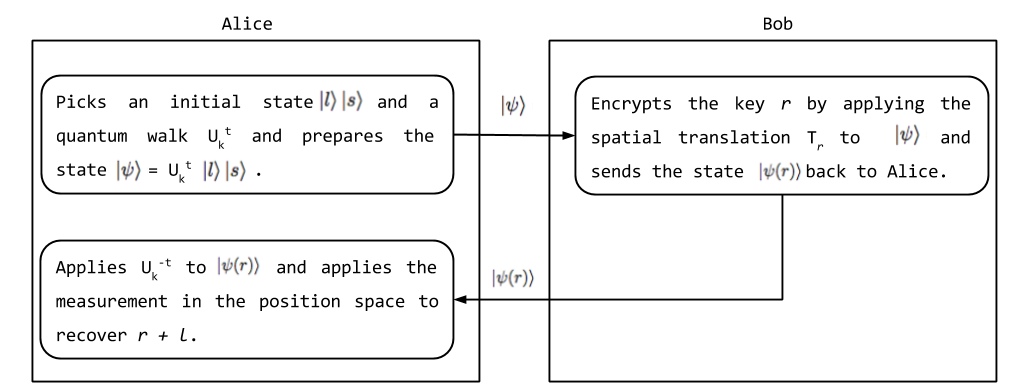
\includegraphics[width=\textwidth]{protocol_QKD.png}
\caption{Description of the basic steps of Protocol~\ref{prot:qkd}.                                     }
\label{fig:protQKD}
\end{figure}
\end{center}


\newpage
\begin{protocol} Quantum key-distribution scheme\
\label{prot:qkd} 
\begin{description}
\item[\hspace{6mm}{\bf Inputs for the protocol}]\
	\begin{itemize}
		\item Key: 

			$r\in \{0, \dots, P-1 \}$, i.e., a key of at most $\log P$ bits, chosen by $B$ uniformly at random;

		\item Quantum state generation:\
		
		The QW operator $U_k$ with $k\in \mathcal K=\{1,2,\ldots,K\}$,
			the number of steps $t \in \mathcal{T} = \{ T_0, \dots, T_{max} \} \subset \mathbb{N},$
		and the initial state $\ket{l}\otimes\ket{s}$, where	$l \in \{ 0, \dots, P-1 \}, $
			$s \in \{R,L\}.$
	\end{itemize}
In the above, $U_k$, the QW operator is defined as $U_k=S\cdot (I_p\otimes R_c (\theta_k))$, where $S$ is the shift operator and $R_c(\theta_k)$ is a rotation of $\theta_k=k\cdot 2\pi/K$ in the coin space.  \vspace{3mm}

\item[\hspace{6mm}{ \bf Quantum state generation} ]\
	\begin{itemize}
	\item $A$ chooses uniformly at random $l \in \{0, \dots ,P-1 \} $ and $s \in\{R,L\}$, and generates the initial state $\Ket{l}\Ket{s}$.
	
	\item Then she chooses, also at random, the QW 
	$U_k=S\cdot \big(I_p\otimes R_c (\theta_k)\big)$ 
	and the number of steps $t\in\mathcal T$.   
	
	\item Finally, she generates the quantum state:
	$$
	\Ket{\psi} 	= U_k^t\Ket{l}\Ket{s} 
				= \big[S\cdot \big(I_p\otimes R_c (\theta_k)\big)\big]^t \Ket{l}\Ket{s},
	$$
	and sends it to $B$.
	\end{itemize}
\vspace{3mm}
\item[\hspace{6mm}{\bf Key encryption} ]\
	\begin{itemize}
	
	\item Upon obtaining the quantum state $\Ket{\psi}$	from $A$, $B$ encrypts the key $r$ by applying spatial translation $T_r=\sum_{i=0}^{P-1}\ket{i + r \pmod{P}} \bra{i}$ to obtain: 
		\[\Ket{\psi(r)} = (T_r\otimes I_c) \Ket{\psi},\] 
		where $I_c$ is the identity operator in the coin space. 
	\item $B$ sends $\Ket{\psi(r)}$ to $A$.
	\end{itemize}
\vspace{3mm}	
	\item[\hspace{6mm}{\bf Key decryption}]\
	\begin{itemize}
	\item $A$ applies $U_k^{-t}$ to the state $\Ket{\psi(r)}$.

	\item She performs the position measurement 
	$$
	M = \sum_{i=0}^{P-1}\Ket{i} \Bra{i}\otimes I_c
	$$ 
	and obtains the result $i_0$. 
	\\The key sent by $B$ is $r= i_0 - l \!\!\pmod {P}$.
\end{itemize}
\end{description}
\end{protocol}

It is clear, from the design of the protocol and the proof of correctness of the QW public-key encryption scheme from Chapter 2 that, if no one interferes with the quantum states, then the protocol is correct and at the end, $A$ and $B$ will share a common string of length $\log P$, that they can use as a key. In the next section we prove the security of the protocol.  


\subsection{Security of the protocol}
\label{sec:sec2way}
Following the same steps as in Section~2.2 of Chapter 2, we can use the Holevo theorem to show that $E$ can extract information about the key, by means of the quantum states $\ket{\psi}$ and $\ket{\psi(r)}$ that $A$ and $B$ exchange, only with negligible probability. However, this is not enough for the case of this  QKD protocol. In the previous public-key cryptosystem, we have silently assumed the existence of a public-key infrastructure, that operates like a trusted third party, as it is usually assumed in public-key cryptography. In QKD though, such an assumption can not be used, therefore we should complete the security analysis, by taking into account full man-in-the-middle attacks. During such an attack, $E$ impersonates $A$ to $B$ and vice versa, while they think that they are communicating directly. This attack gives $E$ the chance to intercept and alter the communication between them. In what follows, we propose two different verification procedures, that allow $A$ and $B$ to verify that what they receive is actually coming from each other and not from an eavesdropper pretending to be either of them. We should note that for both verification methods, $A$ and $B$ need to share a classical public authenticated channel (a common requirement in QKD protocols, such as the well-known BB84 scheme~\cite{ben:bra:84}).


\subsubsection{Standard verification}
\label{sec:stdver}
The first technique we propose is a standard cut-and-choose verification, which is achieved by adding redundancy to our scheme. Clearly, the verification is needed twice in our protocol: once when $A$ sends the QW state to $B$ and once when $B$ sends the encoded key to $A$.\\ 

\textbf{Verification 1}: \textit{$B$ verifies that it was $A$ who sent him the quantum state.}\\
It is needed to prevent $E$ from sending her choice of quantum states to $B$, which would allow her to read the encrypted key while he is sending it back to $A$. 
	\begin{itemize}
		\item $A$ sends to $B$ $\bigotimes_{i=1}^{m}\ket{\psi_i}$, that is, several quantum states $\ket{\psi_i}$, generated by a QW as described in the previous section. Each $\ket{\psi_i}$ is generated using independently chosen walk parameters and initial states $(k_i,t_i,l_i,s_i)$.
			
		\item After $B$ receiving $\bigotimes_{i=1}^{m}\ket{\psi_i}$, $A$, through a classical authenticated channel, sends him a string $v=v_1v_2\ldots v_m$ of $m$ bits, such that $v_i=1$ if the corresponding $\ket{\psi_i}$ is going to be used for verification and $v_i=0$ otherwise, that is, if the corresponding $\ket{\psi_i}$ will be used by $B$ to encode part of the key. Through the classical channel, she also sends $(j,k_j,t_j,l_j,s_j)$, for some uniformly at random chosen $j$'s that belong in the set $\{1,\ldots,m\}$. Let the number of these $j$'s be $m/3$.
		\item $B$ verifies that for all these $j$'s, the received states $\rho_j=\ket{\psi_j}\bra{\psi_j}$ are indeed equal to the pure states 
		$$\Ket{\psi_j} 	= U_{k_j}^{t_{j}}\Ket{l_j}\Ket{s_j}. $$
		In order to verify that, he applies $U_{k_j}^{-t_j}$ to the states $\ket{\psi_j}$, for all $j$ and then performs a measurement for each $j$ in the positions space as well as in the spin space. This measurement (for each $j$) is described by the operator:
		\[
		\begin{array}{rcl}
		M_{l_j,s_j}&=&\ds \sum_{l_j,s_j}\alpha_{l_j,s_j}\ket{l_j,s_j}\bra{l_j,s_j}\\
		&=&\ds \sum_{l_j}l_j\ket{l_j}\bra{l_j}\otimes\sum_{s_j}s_j\ket{s_j}\bra{s_j}.
		\end{array}
		\]
		This way, he traces out all these $\ket{\psi_j}$'s and he is left with $2m/3$ quantum states. We call the reader's attention to the fact that if the verification fails for any $j$, the protocol is stopped.
 		\end{itemize}


\textbf{Verification 2}: \textit{$A$ verifies that it was $B$ who sent her the encrypted key.}\\
This procedure is needed to prevent $E$ from sending to $A$ a message that would decrypt a key different from the one sent by $B$. In this case, $A$ and $B$ would not be able to communicate, while $E$ would be able to decrypt messages sent by $A$. To prevent this from happening, $A$ and $B$ repeat the verification procedure 1, with the roles switched. In particular, the two are performing the following steps:
\begin{itemize}
	\item $B$ encrypts $r_{i}\in \{0,\ldots,P-1\}$ in each of the states of the remaining product state $\bigotimes_{i=1}^{2m/3}\ket{\psi_i}$ as follows:
	 $$\Ket{\psi(r_{i})} = (T_{r_i}\otimes I_c) \Ket{\psi_{i}}, \forall i\in\{1,\ldots,2m/3\}$$
	 that is, translating each state $\ket{\psi_i}$ by $r_i$ in the positions space, leaving the spin part of the state unaltered. 
	 \item He sends the product state $\bigotimes_{i=1}^{2m/3}\Ket{\psi(r_{i})}$ to $A$.
	 \item Then he chooses $m/3 $ uniformly at random $j'$'s out of the $2m/3$ unused indices from the previous verification procedure. Through the classical public authenticated channel he sends a classical string $v'=v'_1v'_2\ldots v'_{2m/3}$ of $2m/3$ bits, such that $v'_i=1$ if the corresponding $\ket{\psi(r_i)}$ is going to be used for verification and $v'_i=0$ otherwise, that is, if the corresponding $\ket{\psi(r_i)}$ contains part of the key. For each $j'$ chosen (for which $v'_i = 1$), he also sends through the classical public authenticated channel the index and the respective $r_{j'}$'s used to generate the state $\ket{ \psi(r_i)}$. 	
	 \item In the last step, $A$ applies $U_{k_i}^{-t_i}$ on the $2m/3$ states $\Ket{\psi(r_i)}$ and then, for each $i$, she performs a measurement on the positions space. Let the outcomes be denoted by $\alpha_i, i\in \{1,\ldots,2m/3\}$. For all the indices she computes $r_i=\alpha_i-l_i,$ where $l_i$ are the initial positions on the circle that she used for the generation of the quantum states $\ket{\psi_i}.$ Finally, for each $j', r_{j'}$ sent by $B$, $A$ verifies the consistency of their results.
	 \item The key is given by the concatenation of the bits $r_i$ that were not used during the two verification procedures and it has $m\cdot (\log P)/3$ bits. Usually, the choice of $m$ is dependent on the desired length, $\log P$, of the key, and in order to make the success probability of a man-in-the-middle attack negligible on $\log P$, it is common to use $m=(\log P)/3$.
\end{itemize}

\subsubsection{Verification using maximally entangled states}
\label{sec:bellver}
In this section, we present an alternative verification procedure, which prevents $E$ from trying to infer the key by first entangling her ancillas with the systems sent by $A$, and then performing an additional operation (say, a measurement) on the joint system of her ancillas and those carrying the encrypted key sent back to $A$ by $B$; a method which in general would give her access to some non-negligible amount of information, so that $A$ and $B$ are not able to securely communicate. 
Note that this verification procedure could also be used against the previous attack in which $E$ simply impersonates $A$ to $B$, and vice versa. \\ During the first step of the protocol (``Quantum state generation''), in addition to generating QW states
\begin{equation}
\label{states:1}
	\ket{\psi}_{qw}=U_k^t\ket{l}\ket{s}
\end{equation}
used to encode the key, for the verification purposes $A$ also creates a number of Bell-like maximally entangled states
\begin{equation}
\label{states:2}
	\ket{\psi}_{qw}=\frac{1}{\sqrt{(\log 2P)!}}\sum_{i=0}^{2P-1}\ket{i}_a\ket{i}_{qw}.
\end{equation}
between the ancilla systems (denoted by $a$) and the QW systems (denoted by $qw$), each of dimension $2P$ (the dimension of the actual QW). At the end of the first step, A sends to B a random sequence of QW states, each either in the form $\ket{\psi}_{qw}$, or $\rho_{qw} = \tr_a\ket{\psi}\bra{\psi}_{qw}$, while keeping the ancillas with her. A also sends through a classical public authenticated channel a classical string $v=v_1\ldots v_n$, where $v_i=0$ if the $i$-th system is going to be used for the encoding of the key, while $v_i=1$ if the $i$-th system is going to be used for verification.\\
The proportion of states used to obtain the key and used for the verification can be chosen in a similar way as in the previous case. Usually, the dimension of the total Hilbert space $2P$ is of the form $2^n$ which, in turn, is isomorphic to the Hilbert space resulting from the  tensor product of $n$ 2-dimensional Hilbert spaces, and thus this state can be written as the tensor product of $n$ standard two-qubit $\ket{\phi^+}$ Bell states.

 After $B$ receives the systems, he and $A$ perform Bell-like measurements on the states meant for the verification and they observe a maximal violation of the Bell's inequalities, since those states are maximally entangled. This way, these states are traced out and $B$ is left with the states~\eqref{states:1} in which he will encode the key (as previously).
 
The same procedure is repeated again, when $B$ sends the encoded key to $A$. He will send a sequence of states, some of the form $(\hat{T}_r\otimes \hat{I}_c)U_k^t\ket{l}\ket{s}$, in which part of the key is encoded and some of the form (4) (with his ancillary system $\ket{i}_B$ maximally entangled to the system sent to $A$), which are going to be used for the verification, as explained above. In the end of the key decryption phase and if all the verifications were okay, $A$ will concatenate the parts of the key to obtain the full key.
 

\subsection{Efficiency and quantum memory requirements}
In Section~2.3 of Chapter 2 we showed that the QW public-key protocol is efficient, i.e., it requires only polynomial time (on the length of the message, say $n$) to transfer $n$ bits of information encoded in $n+1$ qubits. By introducing the verification steps in this QKD scheme we increase the complexity of the system to $n^2$, in order to make the probability of eavesdropping negligible. However, we should notice that, out of this scheme, the size of the key that $A$ and $B$ share at the end is also increased to $n^2/3$, considering $m=n$. Therefore, the number of bits in the key is linear in the number of qubits sent to $B$. As a conclusion, our QKD scheme is efficient, since the complexity increased, but only polynomially.

As already mentioned in Chapter 1, the lack of stable quantum memories is a major issue in quantum cryptography, since it is a practical constraint that is not likely to be solved, at least in the near future. Short-term quantum memories already exist, however it is not always straightforward to argue about the security of a protocol, relying on their existence. In our case, though, things are quite clear. If $E$ does not interfere, $A$ and $B$ do not need quantum memories to execute the protocol, thus the key distribution is independent of such practical constraints. However, the presence of $E$ and the need of verification for $A$ and $B$ introduce memory requirements for {\em all} the parties. 

Below, we present the memory requirements for the case of Section~\ref{sec:stdver}, noting that the case of Section~\ref{sec:bellver} is analogous. To conduct her attack, $E$ needs a stable quantum memory, in order to keep the states she intercepted by $A$, while waiting for $B$ to encrypt and send the key. Subsequently, she will encode it in $A$'s states and send it to her. Also, in this scenario, $A$ and $B$ need a quantum memory, in order to perform the verification. They need to save the quantum states for some time, while waiting for the other party to send the classical information. Observe that $E$'s memory should be more stable than $A$'s and $B$'s, as the time $E$ needs to save the quantum states for, is clearly longer than the time that $A$ and $B$ need for the same purpose.

Hence, we conclude that our QKD scheme is  secure, as long as $A$ and $B$ have at least as powerful equipment as the adversary $E$. Obviously, if the adversary is technologically more advanced, then virtually any real-life implementation of a security protocol becomes potentially vulnerable.

\section{One-way quantum key distribution protocol}
\label{sec:oneway}
In this section, we propose a one-way QKD protocol, where again the key is encoded in a QW state.
As opposite to the previous two-way protocol, where both $A$ and $B$ perform QW operations, in this case it is only $A$ that chooses randomly the precise QW to encode the key, while $B$ is randomly choosing in which basis (computational or QW) to measure. After disclosing their choices by means of classical communication, they are able to establish a shared key. We will first present the protocol in its PM form and then we will prove its security against general attacks by considering an equivalent EB protocol. The PM form of the protocol is depicted in Figure~\ref{fig:prot1}.\\


\begin{center}
\begin{figure}[h!]
  \centering
  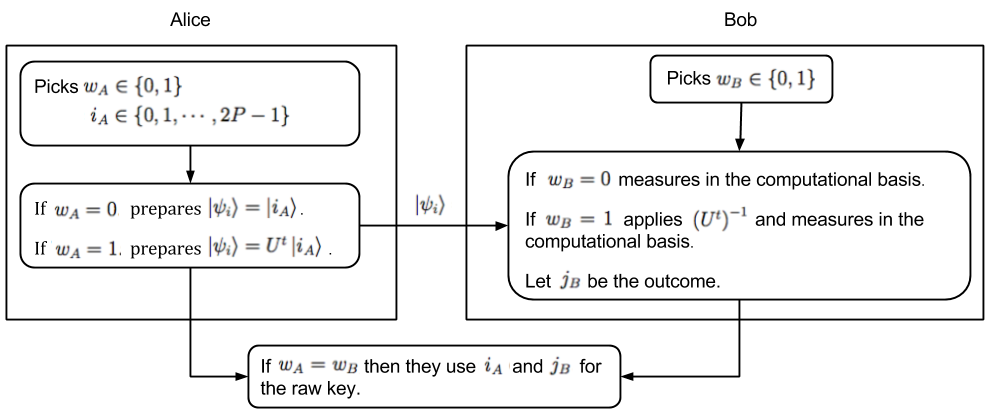
\includegraphics[width=\textwidth]{protocol_one-way.png}
\caption{Description of the basic steps of Protocol~\ref{alg:prot1}.}
\label{fig:prot1}
\end{figure}
\end{center}



\begin{protocol}
\label{alg:prot1}
Let $\theta_k, t,$ and $P$ be publicly known where $P$ is the dimension of the position space of the QW, $t$ is the number of steps to perform the QW, and $\theta_k$ the coin parameter (see Section~\ref{sec:secpk} for the exact form of $\theta_k$).  Let $U_k$ be the QW operator $U_k = S\cdot (I_p\otimes R_c(\theta_k))$ that is also known by the parties (i.e., it is also publicly known) and let $F$ be an operator acting only on $\mathcal{H}_c$. $F$'s action is to ``flip'' the coin to some initial state before evolving the walk and is optional (in which case $F=I_c$). Finally, let $\ket{\psi_i} = U_k^t(I_p\otimes F)\ket{i}$ for $\ket{i} \in \mathcal{H}_p\otimes\mathcal{H}_c$.  We call the orthonormal basis $\{\ket{\psi_i}\}$ the QW basis and denote the computational basis by $Z$.


The protocol consists of $N$ iterations of the following steps:
\begin{enumerate}
  \item $A$ picks a random bit $w_A \in \{0,1\}$ and a value $i_A \in \{0,1, \cdots, 2P-1\}$.
    \begin{itemize}
    \item If $w_A = 0$: $A$ will prepare and send to $B$ the $2P$-dimensional state $\ket{\psi_i} = \ket{i_A}$.
    \item If $w_A = 1$: $A$ will prepare and send to $B$ the $2P$-dimensional state $\ket{\psi_i} = U_k^t(I_p\otimes F)\ket{i_A}$.
    \end{itemize}

  \item $B$ picks a random bit $w_B \in \{0,1\}$.
    \begin{itemize}
    \item If $w_B = 0$: $B$ measures the received $2P$ dimensional state in the computational $Z$ basis resulting in outcome $j_B$.
    \item If $w_B = 1$: $B$ measures in the QW basis (alternatively, he inverts the QW by applying $\left(U_k^t\right)^{-1}$ and measures the resulting state in the $Z$ basis).  The result is translated, in the obvious way, into an integer $j_B$.
    \end{itemize}
Note that he measures both the position and coin, as opposite to the previous protocol, where the measurement for the key was only on the positions space.
  \item $A$ and $B$ reveal, via the authenticated classical channel, their choice of $w_A$ and $w_B$.  If $w_A = w_B$, they will use their values $i_A$ and $j_B$ to contribute towards their raw key.  Otherwise, if $w_A \ne w_B$, they will discard this iteration.
\end{enumerate}

After the above process, $A$ and $B$ will use a cut-and-choose technique similar to Yao's ~\cite{yao:86}, to check eavesdropping by choosing a suitable subset of non-discarded iterations for parameter estimation in the usual manner (discarding those chosen iterations from the raw key). This allows them to estimate the disturbance $Q_Z$ and $Q_W$ in the $Z$ and QW bases respectively (i.e., in the absence of noise $Q_Z = Q_W = 0$).  If this disturbance is ``sufficiently low'' (to be discussed below) the users proceed with error correction and privacy amplification in the usual manner.

\end{protocol}
\subsection{Security of the protocol}

In order to prove the security of Protocol~\ref{alg:prot1}, we will construct, in the usual way, an equivalent EB protocol~\cite{ben:bra:mer:92,lo:cha:99}. Proving security of this EB protocol will show the security of the PM version. For this EB version, for each one of the $N$ iterations, we make changes to steps (1) and (2), replacing them as follows:\vspace{5mm}

\textbf{New Step (1)}: $A$ prepares the entangled state:
\[
\ket{\phi_0} = \frac{1}{\sqrt{2P}}\sum_{i=0}^{2P-1}\ket{i,i}_{AB}
\]
which lives in the $4P^2$ dimensional Hilbert space: $\left(\mathcal{H}_p\otimes\mathcal{H}_c\right)^{\otimes 2}$.  She sends the second half (the $B$ portion of $\ket{\phi_0}$) to $B$ while keeping the first half (the $A$ portion) in her private lab. \vspace{5mm}

\textbf{New Step (2)}: $A$ and $B$ choose independently two random bits $w_A$ and $w_B$.  If $w_A = 0$, $A$ will measure her half of the entangled state in the computational $Z$ basis; otherwise she will measure her half in the QW basis.  Similarly for $B$ and $w_B$.  Let their measurement results in values be $i_A$ on $A$'s side and $j_B$ on $B$'s side.

We now show the security of this entanglement-based version of the protocol.  In the following proof, we will initially make three assumptions:
\begin{enumerate}
  \item[\bf A1:] $A$ and $B$ only use those iterations where $w_A = w_B = 0$ for their raw key.

  \item[\bf A2:] $E$ is restricted to collective attacks (those whereby she attacks each iteration of the protocol independently and identically, but is free to perform a joint measurement of her ancilla at any future time of her choosing).

  \item[\bf A3:] $E$ is the party that actually prepares the states which $A$ and $B$ hold.
\end{enumerate}

Assumption A1 is made only to simplify the computation and may be discarded later (alternatively, one may bias the basis choice so that $w_A$ and $w_B$ are chosen to be $0$ with high probability, thus increasing the efficiency of the protocol as is done for instance for BB84 in~\cite{lo:cha:ard:05}).  Assumption A2 may be removed later using a de Finetti-type argument~\cite{ren:gis:kra:05,chr:kon:ren:09,ren:07} (in this paper, we are only concerned with the asymptotic scenario, so the key-rate expression we derive will not be degraded). Note that removing A2 gives us the security. Assumption A3 gives greater advantage to the adversary; if we prove security using A3, then the ``real-world'' case, where assumption A3 is not used, will certainly be just as secure, if not even more.

In light of A2 and A3, $A$, $B$, and $E$, after $N$ iterations of the protocol, hold a quantum state $\rho_{ABE}^{\otimes N}$, where $\rho_{ABE} \in \mathcal{H}_A\otimes\mathcal{H}_B\otimes\mathcal{H}_E$ with $\mathcal{H}_A \equiv \mathcal{H}_B \equiv \mathcal{H}_p\otimes\mathcal{H}_c$.  Following error correction and privacy amplification, $A$ and $B$ will hold a secret key of size $\ell(N)$.  Under the assumption of collective attacks (A2), we may use the Devetak-Winter key-rate expression~\cite{dev:win:05} to compute:
\[
r = \lim_{N\rightarrow \infty}\frac{\ell(N)}{N} = S(A|E) - H(A|B).
\]

Let $A_Z$ and $A_W$ be the random variables describing $A$'s system, when she measures in the $Z$ or $QW$ basis, respectively.  Similarly, define $B_Z$ and $B_W$.  Under assumption A1, we are actually interested in the value:
\[
r = S(A_Z|E) - H(A_Z|B_Z).
\]

Computing $H(A_Z|B_Z)$ is trivial, given the observable probabilities:
%
\begin{equation}\label{eq:prot1:probZ}
p^Z_{i,j} = Pr(i_A=i \text{ and } j_B=j \text{ } | \text{ } w_A=w_B=0).
\end{equation}
%
The challenge is to determine a bound on the von Neumann entropy $S(A_Z|E)$.

To do so, we will use an uncertainty relation, proven in~\cite{ber:chr:col:ren:ren:10}, which states that for any density operator $\sigma_{ABE}$ acting on Hilbert space $\mathcal{H}_A\otimes\mathcal{H}_B\otimes\mathcal{H}_E$, if $A$ and $B$ make measurements using POVMs $\mathcal{M}_0 = \left\{M_x^{(0)}\right\}_x$ or $\mathcal{M}_1 = \left\{M_x^{(1)}\right\}_x$, then

\begin{equation}
S(A_0|E) + H(A_1|B) \ge \log\frac{1}{c},
\end{equation}

where

\begin{equation}
c = \max_{x,y}\left|\left| M_x^{(0)}M_y^{(1)} \right|\right|_\infty^2
\end{equation}
where we take $||\cdot||_\infty$ to be the operator norm and $A_i$ to be the random variable describing $A$'s system after measuring $\mathcal{M}_i$ (we will later, similarly, define $B_i$). Assuming measurements $\mathcal{M}_0$ are used for key distillation, simple algebra, as discussed in~\cite{ber:chr:col:ren:ren:10}, yields the Devetak-Winter key-rate:
\begin{eqnarray*}
r = S(A_0|E) - H(A_0|B_0)& \ge &\log\frac{1}{c} - H(A_0|B_0) - H(A_1|B)\\[2mm]
&\ge & \log\frac{1}{c} - H(A_0|B_0) - H(A_1|B_1).
\end{eqnarray*}
The last inequality follows from the basic fact that measurements can only increase entropy.

In our case, we have $M_x^{(0)} = \ket{x}\bra{x}$ and $M_x^{(1)} = \ket{\psi_x}\bra{\psi_x}$ for $x \in \left\{0, 1, \cdots, 2P-1\right\}$.  Let $\ket{\psi_x} = \sum_{i=0}^{2P-1}\alpha_{x,i}\ket{i}$; then it is easy to see that for all $x,y$
\[
\left|\left|M_x^{(0)}M_y^{(1)}\right|\right|_\infty^2 = |\alpha_{y,x}|^2,
\]
and therefore
\begin{equation}\label{eq:prot1:cval}
c = \max_{x,y}|\alpha_{x,y}|^2,
\end{equation}
a quantity which depends exclusively on the choice of the QW parameters and not on the noise in the channel. 
Therefore, $A$ and $B$ should choose optimal $t, \theta_k$ and $P$ in order to minimise $c$ (thereby maximising the key-rate equation).
As we will show in the next section, this analysis is sufficient to derive good key-rate bounds.

\subsection{Evaluation}
As mentioned above, the value of $c$ depends solely on the QW parameters which are under $A$ and $B$'s control; therefore it is to their advantage to choose a QW which minimises this value (i.e., such that, after evolving for $t$ steps, the probability of finding the walker at any particular position is small). 

 It is easy to see that, as $t \rightarrow \infty$, the values $|\alpha_{x,y}|$ do not converge to a steady state which is why, usually, one considers the time-averaged distribution when analysing QWs on the cycle~\cite{aha:amb:kem:vaz:01,kem:03}. 

However, in our QKD protocol, we do not care what happens at large $t$; instead, we wish to find an optimal $t$ and one that is preferably not ``too large'' (the larger it is, the longer, in general, it might take $A$ to prepare the state and $B$ to reverse it).

We begin by looking at various walk parameters and finding the minimal value of $c$ when $F=I_c$, the identity operator. Note that, on the circle, it makes sense only to consider odd $P$ as even $P$ would force the support of the probability amplitudes onto even or odd numbered nodes only thereby increasing the overall value of $|\alpha_{x,y}|$. We wrote a computer program to simulate the walk for time steps $t = 1, 2,\cdots , T_{\text{max}}$ (for user-specified value $T_{\text{max}}$) searching for the optimal value of $t$ (i.e., a value for $t$ whereby $c$ is minimum). For the evaluation we used a more general form of the coin rotation operator:

\begin{equation*}
R_c(\theta,\phi) = 	\left( 
				\begin{array}{cc}
					e^{i\phi} \cos(\theta) & e^{i\phi} \sin(\theta) \\
					-e^{-i\phi} \sin(\theta)& e^{-i\phi} \cos(\theta)
				\end{array}
			\right),
\end{equation*}

The results for $\theta = \pi/4, \phi = 0$, and for various $P$ are shown in Figure~\ref{fig:prot1:cvals}.
	
\begin{figure}[h!]
  \centering
  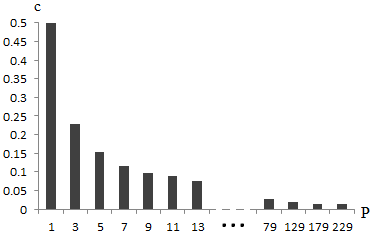
\includegraphics[scale = 0.6]{overlap-piover4.png}
\caption{Showing minimal value of $c$ found by our program for given position space dimension $P$ when $\theta = \pi / 4,\phi=0$ and $F=I_c$.  When $P \le 13$ we set $T_{\max} = 5000$; when $P \ge 79$ we set $T_{\max} = 50000$.  Note that, the smaller $c$ is, the better for $A$ and $B$.  Note also that $P$ is the dimension of the position space, \emph{not} the number of qubits sent which would actually be $\lceil\log P\rceil+1$ (where the extra ``$+1$'' is due to the coin).}\label{fig:prot1:cvals}
\end{figure}


Now that we can find the optimal choice of QW parameters for particular values of $P$ and, more importantly for our work here, the resulting value of $c$. To this end, we have to compute our bound $r$ and determine for what noise levels we can have $r > 0$.  
In practice, one would observe values $p_{i,j}^Z$ and $p_{i,j}^W$ (see Equation~\eqref{eq:prot1:probZ} and define $p_{i,j}^W$ analogously) and use these to directly compute $H(A_Z|B_Z)$ and $H(A_W|B_W)$ as required by the key-rate equation.  For the purpose of illustration in this paper, however, we will evaluate our key-rate bound assuming a generalised Pauli channel as discussed in~\cite{bae:aci:07} (see, in particular, Section~7 of that source). This channel maps an input state $\rho$ to an output state $\mathcal{E}(\rho)$ defined as:
\begin{equation}\label{eq:prot1-channel}
\mathcal{E}(\rho) = \sum_{m=0}^{2P-1}\sum_{n=0}^{2P-1}p_{m,n}\;\mathcal{U}_{m,n}\;\rho\;\mathcal{U}_{m,n}^*,
\end{equation}
where:
\begin{equation}
\mathcal{U}_{m,n} = \sum_{k=0}^{2P-1}e^{{\pi \cdot i \cdot  k \cdot n}/{P}}\ket{k+m}\bra{k},
\end{equation}
That is, this channel $\mathcal{E}(\cdot)$ models an adversary's attack which induces phase and flip errors with probabilities denoted by $p_{m,n}$.  In our numerical computations to follow, we will use:
\begin{equation}\label{eq:prot1-channelpr}
p_{i,j} = \left\{
\begin{array}{ll}
	1-E_r & \text{ if } i = j = 0\\[4mm]
	\ds \frac{E_r}{(2P)^2-1} & \text{ otherwise}
\end{array}
\right. .
\end{equation}
It is clear that $\sum_{i,j}p_{i,j} = 1$.  Furthermore, when $E_r=0$, we have $\sum_ip_{i,i}^Z = \sum_ip_{i,i}^W = 1$ (i.e., there is no disturbance in the channel) while as $E_r$ increases, the disturbance also increases.

Finally, we define the total noise in the channel to be:
\[
Q = \sum_{a\ne b}p_{a,b}^Z = \sum_{a\ne b} Pr \big( A_Z=a \text{ and } B_Z = b \text{ } | \text{ } w_A = w_B = 0 \big).
\]
That is to say, $Q$ represents the quantum error rate (QER) of the channel.

The maximally tolerated QER, for those QWs analysed in Figure~\ref{fig:prot1:cvals}, and using the above described noise model, is shown in Figure~\ref{fig:prot1:maxnoise1}.  Note that, when $P=1$ and $t=1$, we recover the BB84 limit of $11\%$ which is to be expected since, with these choice of parameters, we are essentially running the BB84 protocol.
\begin{figure}[h!]
  \centering
  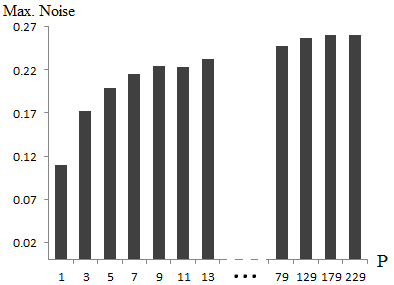
\includegraphics[scale=0.6]{maxNoisePiOver4.png}
\caption{Showing the maximally tolerated noise level for our protocol using parameters found in Figure~\ref{fig:prot1:cvals} and using the quantum channel described by Equations~\eqref{eq:prot1-channel} and~ \eqref{eq:prot1-channelpr}. The lack of increase in noise tolerance from $P=9$ to $P=11$ (while other choices caused an increase) indicates that $T_{\max}$ was too low.  Note that, when $P = 1$, we recover the BB84 tolerance of $Q = 0.11$ as expected.  Also note that, when $P = 229$, the maximal tolerated noise is $Q = 0.261$.}\label{fig:prot1:maxnoise1}
\end{figure}
Observe in Figure~\ref{fig:prot1:maxnoise1} that there is a lack of increase when $P=9$ and $P=11$; this indicates that our choice of $T_{\max} = 5000$ was too low.  Running our simulator again with $T_{\max} = 50000$ for these small $P$ values yields a maximally tolerated noise level shown in Figure~\ref{fig:prot1:maxnoise2}.

\begin{figure}[h!]
  \centering
  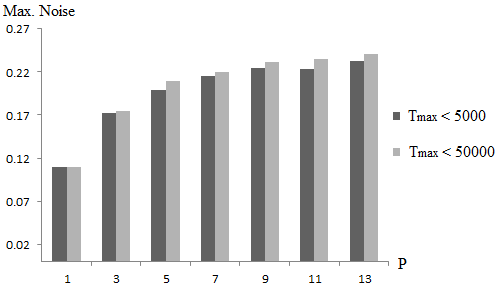
\includegraphics[scale=0.60]{maxNoiseBigT.png}
\caption{Comparing the maximally tolerated noise when $t$ is allowed to be as large as $50000$ (light gray) or only $5000$ (dark grey); again when $F = I$ and $\phi = 0$.  In this case, when $P=13$ and $T_{\max} = 50000$, the maximal tolerated noise $Q$ is $Q = 0.241$.}\label{fig:prot1:maxnoise2}
\end{figure}

Finally, we re-run the simulator, using $T_{\max} = 5000$ and $T_{\max} = 50000$ for a different QW parameter of $\theta = \sqrt{2}\pi/4$ which, for these particular upper-bounds on $t$ yield a higher tolerated noise as shown in Figures~\ref{fig:prot1:walk2} and\ref{fig:prot1:walk2-2}.  
We comment that, if $T_{\max}$ were larger, the two QWs may produce a QKD protocol with the same tolerated noise; however for these ``smaller'' bounds on $t$ the QW with parameter $\theta = \sqrt{2}\pi/4$ produces a more secure protocol than when $\theta = \pi/4$.  Since smaller $t$ implies a more efficient protocol, this is an advantage.  This opens two very interesting questions: first, do these QWs produce equivalent noise tolerances as $T_{\max}\rightarrow \infty$? Second, what other values of $\theta$ produce even more secure QKD protocols for small $T_{\max}$?  We comment that we also ran this numerical experiment for $\theta = \pi/5$ and $\theta = \pi/3$ but got worse noise tolerances.

\begin{figure}[h!]
  \centering
  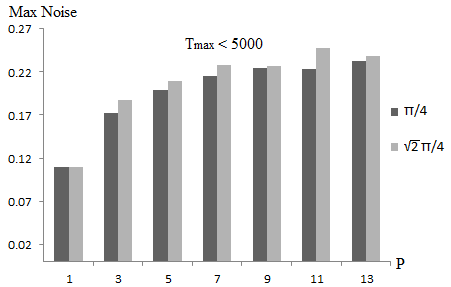
\includegraphics[scale = 0.60]{maxNoiseCompare.png}
\caption{Comparing the maximal tolerated noise levels of the QKD protocol when $\theta = \pi/4$ (dark gray) and $\theta = \sqrt{2}\pi/4$ (light grey).  In this chart, $T_{\max} = 5000$ which, observing the ``drop'' in tolerated noise when $P$ goes from 11 to 13, is too small.  See also Figure~\ref{fig:prot1:walk2-2} for the same chart when $T_{\max} = 50000$.}\label{fig:prot1:walk2}
\end{figure}

\begin{figure}[h!]
  \centering
  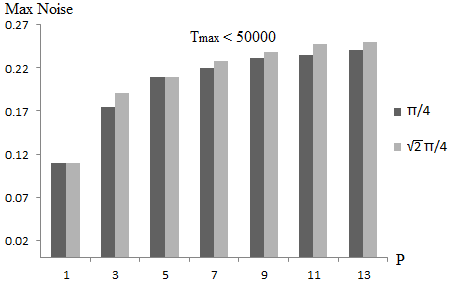
\includegraphics[scale = 0.60]{maxNoiseCompareBigT.png}
\caption{Comparing the maximal tolerated noise levels of the QKD protocol when $\theta = \pi/4$ (dark gray) and $\theta = \sqrt{2}\pi/4$ (light grey).  In this chart, $T_{\max} = 50000$.  In all cases, the QW parameter $\theta = \sqrt{2}\pi/4$ produces a more secure QKD protocol for this upper-bound on $t$.  Note that, as $T_{\max} \rightarrow \infty$, they may produce equally secure protocols; this, as discussed in the text, is an open question.  In this case, when $P=13$ and $\theta = \sqrt{2}\pi/4$, the maximally tolerated noise is $0.25$ (compared to $0.241$ when $\theta = \pi/4$).}\label{fig:prot1:walk2-2}
\end{figure}


From the above it is clear that careful choice of the QW parameters is vital for producing a QKD protocol tolerant of high noise channels.  To investigate this further, we simulate the QW for all $\theta,\phi \in \{k\pi/10 \text{ } | \text{ } k = 0, 1, \cdots, 10\}$.  Furthermore, for each setting, we also consider the use of $F = I, F = X$, and $F = Y$, where:
\[
\begin{array}{clc}
X = \ds \frac{1}{\sqrt{2}}\left(
			\begin{array}{cc}
					1 & 1\\
					1 & -1
			\end{array}\right)
& &
Y = \ds \frac{1}{\sqrt{2}}\left(
			\begin{array}{cc}
					1 & 1\\
					i & -i
			\end{array}\right).
\end{array}
\]	


For each setting, we find the optimal choice of time $t \le 5000$ which produces a minimal $c$.  We then take this value and determine the highest disturbance the resulting protocol can withstand.  The respective data is summarised in Table~\ref{table:sim-results}.

\begin{center}
	\begin{table*}[h!]
		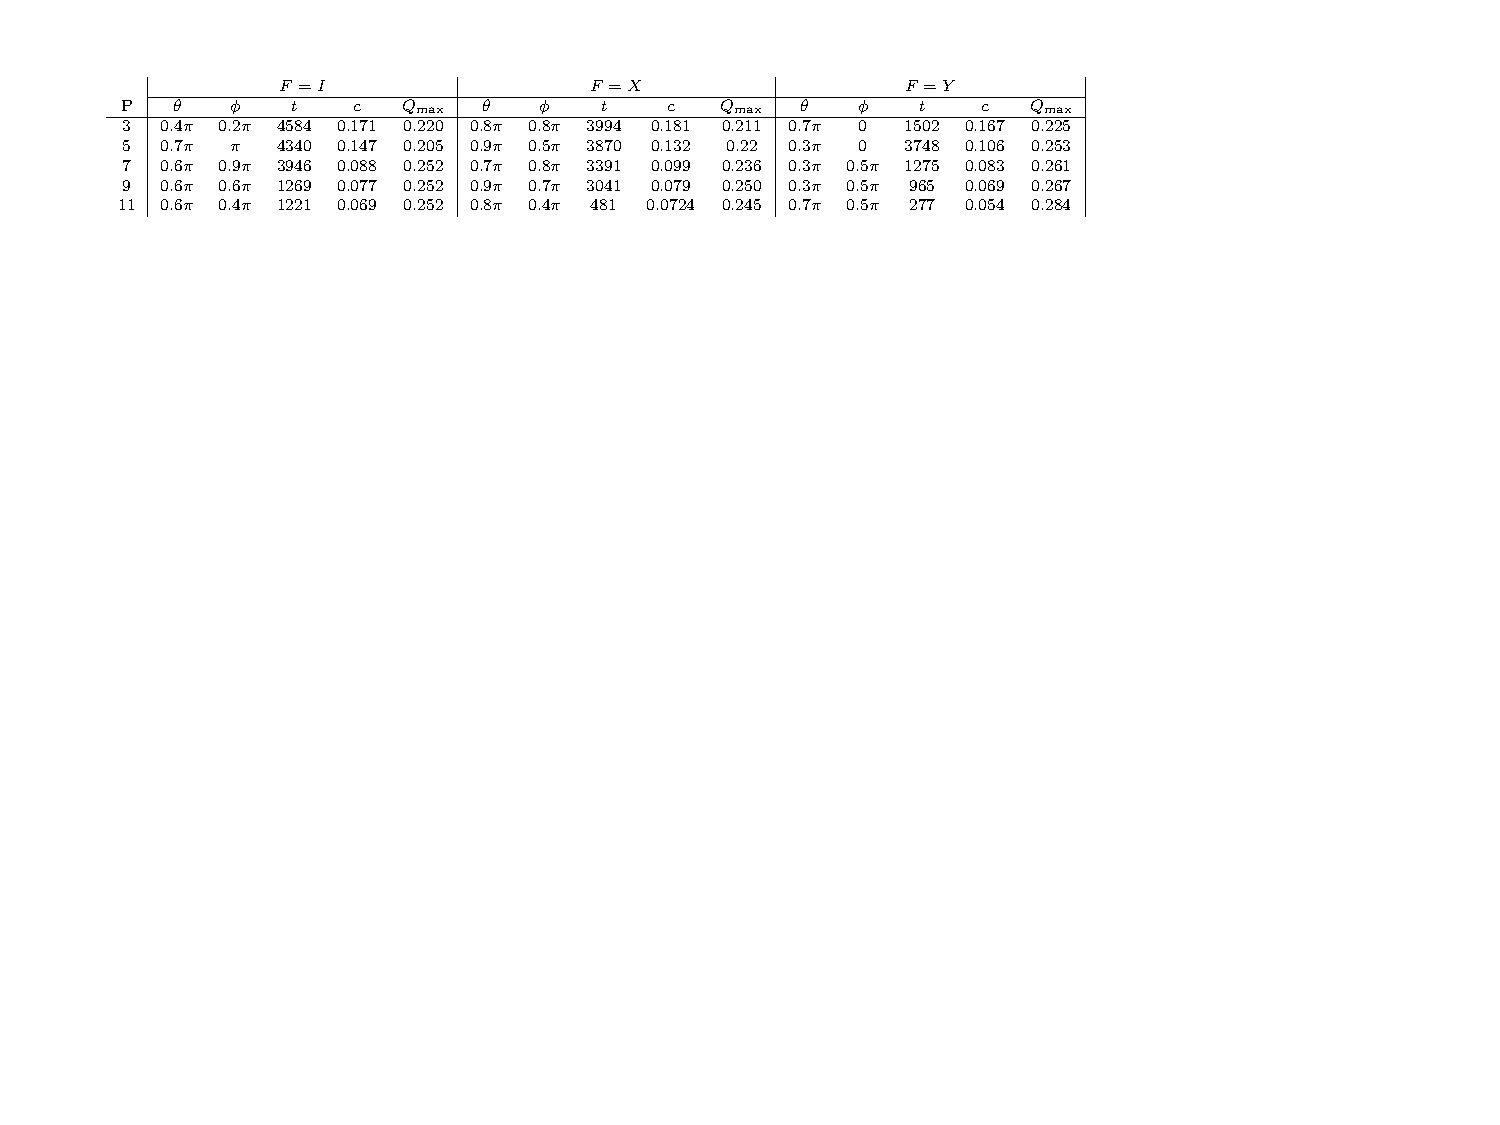
\includegraphics[scale = 1.1]{Table1}
		\caption{Showing the optimal choice of QW parameters to maximise the noise tolerance ($Q_{\text{max}}$) of the resulting protocol.  For this data, we searched for QWs with at most $T_{\text{max}} = 5000$ steps and with parameters $\theta,\phi \in \{k\pi/10 \text{ } | \text{ } k = 0, 1, \cdots, 10\}$.}\label{table:sim-results}
	\end{table*}
\end{center}

Note that, for some data points (e.g., when $P = 5$ and $F = I$) there is a drop in the maximum tolerated noise.  This is a consequence either of setting $T_{\text{max}}$ too small, or we need to simulate more QW parameters. For example, when we set $T_{\max} = 50000$, for $P = 5$ and $F = I$, we get a maximum noise tolerance of $0.236$ when $t = 40847$.  Note also, that setting $F = Y$ achieves the best result for this test, $Q_{\text{max}}=0.284$.\\

In Table~\ref{table:sim-results2}, we carried out the same experiment, however this time searching over QW parameters in the set $\theta, \phi \in \{k\pi/20 \text{ } | \text{ } k = 0, 1, \cdots, 20\}$. Again, the best result for this case is $Q_{\text{max}}=0.284$ and is achieved when considering $F = Y$. 

\begin{center}
	\begin{table*}[h!]
		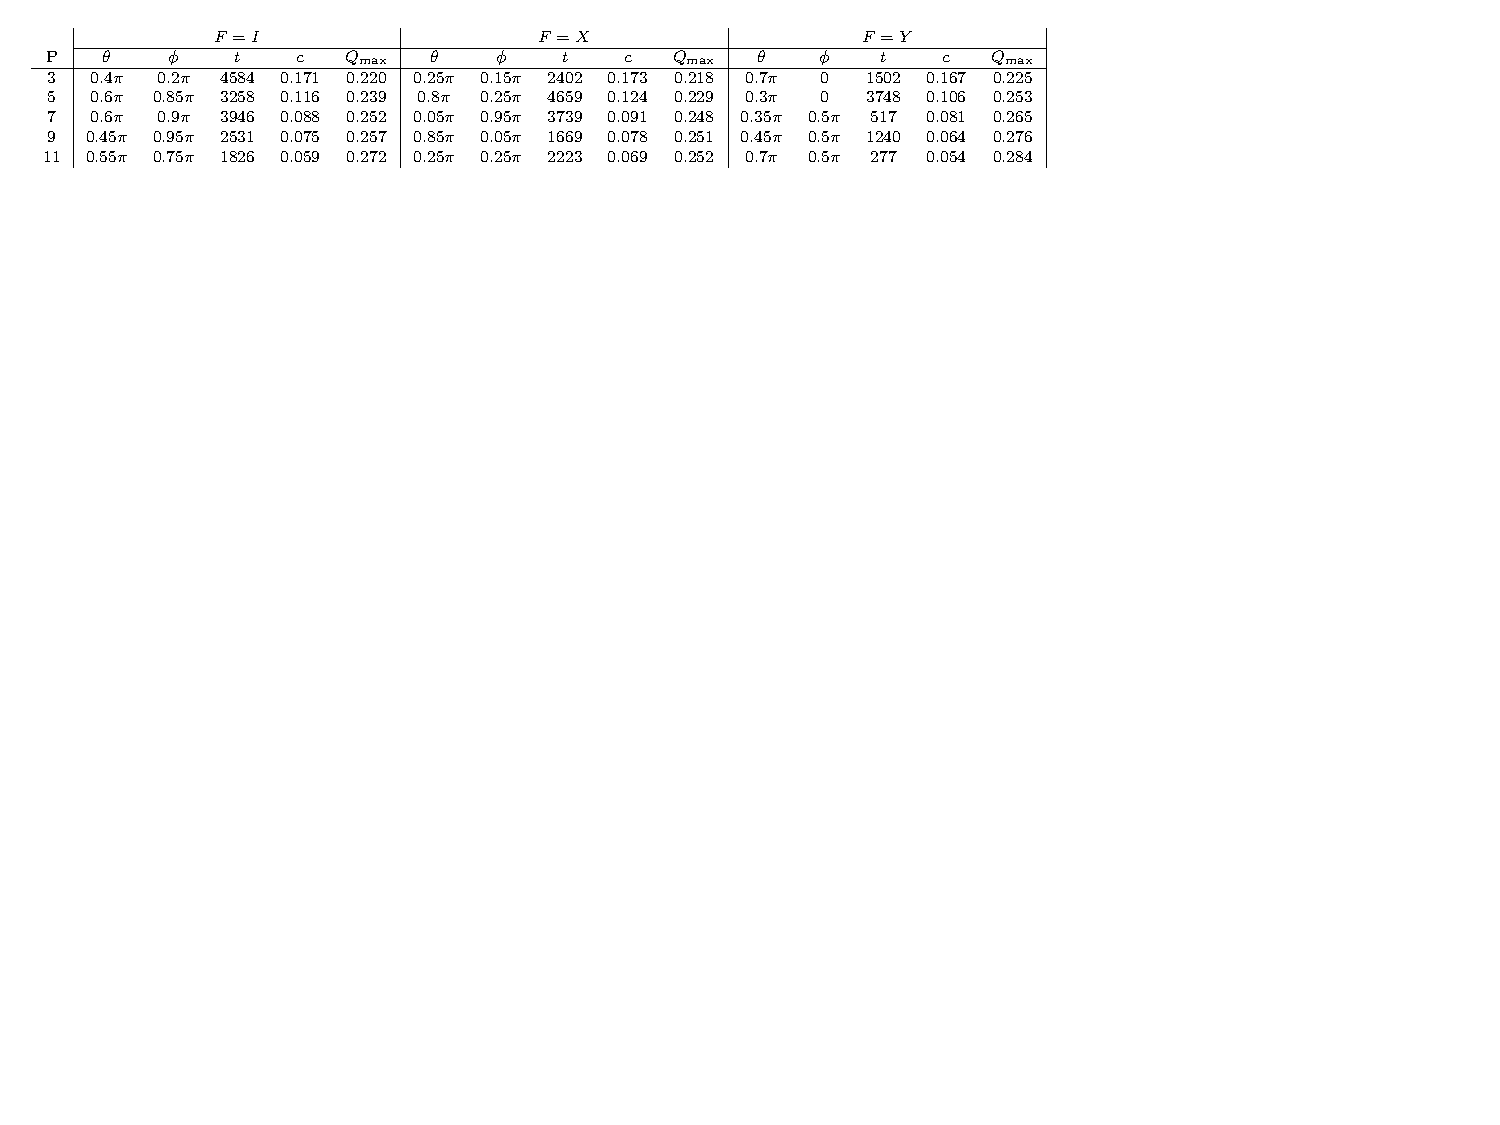
\includegraphics{Table2.pdf}
		\caption{Showing the optimal choice of QW parameters to maximise the noise tolerance ($Q_{\text{max}}$) of the resulting protocol.  For this data, we searched for QWs with at most $T_{\text{max}} = 5000$ steps and with parameters $\theta,\phi \in \{k\pi/20 \text{ } | \text{ } k = 0, 1, \cdots, 20\}$.}\label{table:sim-results2}
	\end{table*}
\end{center}

As mentioned at the beginning of this section, all the numerical results were obtained by simulating the evolution of the QW on a custom QW simulator that we wrote. However, we also verified the results through an alternative technique, namely by computing the probability amplitudes of the QW using the standard Fourier method (see, e.g.~\cite{nay:vis:00,ven:and:12}) of analysing QWs. The results obtained by both methods agree with each other.\\

Finally, we note that the protocol's security is not compromised by considering the existence or not of quantum memories. It is sufficient to consider the PM form of the protocol. $E$ needs a quantum memory to perform her attack, as she needs to save her ancillary system throughout the execution of the protocol. In the contrary, the secure key distribution between $A$ and $B$ does not require any quantum memory. Therefore, if $E$ does not have a quantum memory she cannot attack, while if even she has one and attacks, $A$ and $B$ can defend against it and securely share a key at the end. Notice, that even if we consider the EB version of the protocol, again the security is independent of any quantum memory requirements, as $E$ for her attack needs a more stable quantum memory than $A$ and $B$ need to defend against it and securely distil the key.  

\newpage

\section{Semi-quantum key distribution protocol}
\label{sec:semi-qkdscheme}

As a third contribution, in this section, we propose a new \emph{semi-quantum} key-distribution (SQKD) protocol based on QWs.  The concept of semi-quantum cryptography was introduced by Boyer {\em et al.}~\cite{boy:ken:mor:07,boy:gel:ken:mor:09}, as a way to study ``how quantum'' does a protocol need to be in order to surpass the security of its classical counterparts -- namely, how ``quantum'' do the parties need to be in order to establish a secret key secure against an all-powerful adversary.  A semi-quantum protocol places restrictions on one of the participating users (typically $B$) in that he may only operate in a ``classical'' or ``semi-quantum'' manner. In particular, this limited user -- usually called the {\em classical party} -- can only directly work with the computational basis.  No restrictions are placed on $A$, who is fully quantum, i.e., she possesses quantum equipment and can perform quantum operations and of course, no restrictions are placed on $E$. Implementation-wise, such protocols can be seen as practical instances of QKD, since they involve less quantum hardware. 
 Semi-quantum protocols rely on a two-way quantum channel allowing a quantum state to travel from $A$ to $B$, and then back to $A$.  When first introduced by Boyer {\em et al.} in \cite{boy:ken:mor:07}, these classical operations involved $B$ either measuring the incoming qubit in the $Z = \{\ket{0}, \ket{1}\}$ basis, or reflecting the incoming qubit, bouncing it back to $A$ undisturbed.  For our purposes, we extend this definition of ``classical'' operations to operate with higher dimensional systems.  As we do not want to restrict ourselves necessarily to qubit encodings (and thus, dimensions that are powers of two), we will say that $B$, on receipt of an $D$ dimensional quantum state $\ket{\psi},$ may choose to do one of two operations:
\begin{enumerate}
  \item Measure and Resend: $B$ may subject the $D$-dimensional quantum state to a measurement in the computational basis spanned by states: $\{\ket{0}, \ket{1}, \cdots,$ $ \ket{D-1}\}$.  He will then prepare a new $D$-dimensional quantum state in this same computational basis based on the result of his measurement.  Namely, if he observes $\ket{r}$ for $r \in \{0, 1, \cdots, D-1\}$, he will send to $A$ the quantum state $\ket{r}$.
  \item Reflect: $B$ may ignore the incoming $D$-dimensional quantum state and reflect it back to $A$.  In this case he learns nothing about its state.
\end{enumerate}

With these restrictions on the part of the classical user defined, we now depict our protocol in Figure~\ref{fig:semi_QKD} and describe it immediately below.


    \begin{center}
    \begin{figure}[h!]
    \centering
    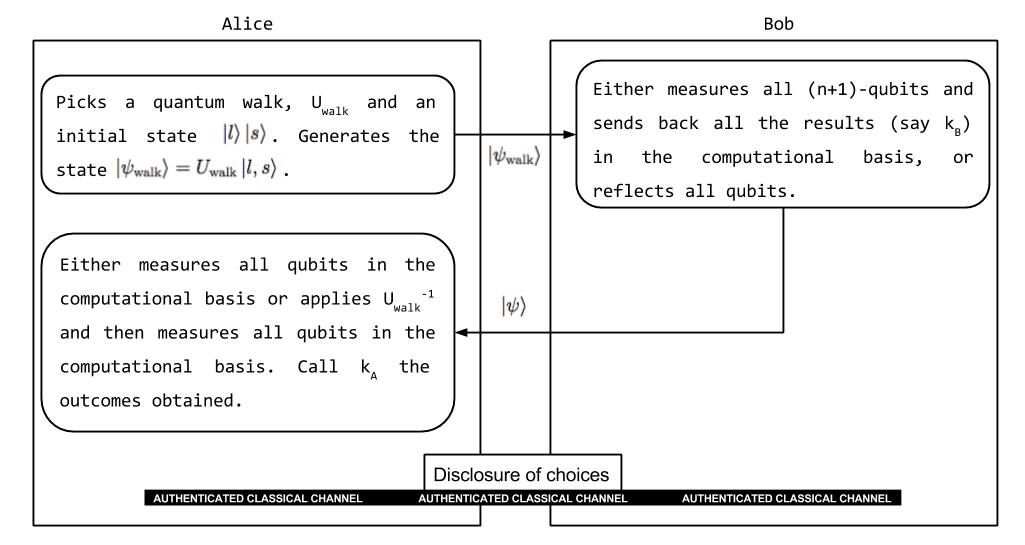
\includegraphics[width=0.8\textwidth]{semi_quantum_QKD.png}
    \caption{Description of the basic steps of Protocol~\ref{prot:semi-q}.}
    \label{fig:semi_QKD}
    \end{figure}
    \end{center}

\newpage
\begin{protocol} Semi-quantum key-distribution scheme\
\label{prot:semi-q} 
\begin{description}
\item[\hspace{6mm}{\bf Inputs for the protocol} ]\
\begin{itemize}
	\item $\ket{l,s}$, the initial state of the QW, where $l \in \mathcal L=\{ 0, \dots, P-1 \} $ is the initial position of the walker, and $s \in \mathcal S=\{R,L\}$ gives the initial coin state.
	\item $U_{\textnormal{walk}} = (U_k)^t \in \mathcal Q$, the evolution of the QW, where $k \in \mathcal K  =\{1,2,\ldots,K\}$ is the choice of a single step unitary $U_k$, and $t \in \mathcal{T} = \{ T_0, \dots, T_{max} \}$ is the number of steps of the QW. Thus, $\mathcal Q$ is the set of all possible QWs. Note that $\mathcal Q$  is publicly known.
\end{itemize}

\vspace{3mm}
\item[\hspace{6mm}{\bf Quantum state Generation}]\
\begin{itemize}
 \item $A$ chooses uniformly at random $l \in \mathcal L=\{0,1,\cdots, P-1\}$ and $s\in\mathcal S=\{R,L\}$.  She also chooses a random QW operator $U_{\textnormal{walk}} \in \mathcal{Q}$ according to a publicly known distribution (e.g., uniform).  She then prepares the following state:

$$\ket{\psi_{\textnormal{walk}}} = U_{\textnormal{walk}}\ket{l,s}.$$
\item $A$ sends this state to $B$.
\end{itemize}

\vspace{3mm}
 \item[\hspace{6mm}{ \bf Classical operations by $B$} ]\
 
 
  $B$ chooses either to measure-and-resend the quantum state in the computational basis $\{\ket{0}, \ket{1}, \cdots, \ket{2P-1}\}$ (note that, in this protocol as well, he measures both the position and coin in order to obtain the key, thus his measurement, and subsequent preparation, is of dimension $2P$); or he will reflect the quantum state back to $A$.

\vspace{3mm}

  \item[\hspace{6mm}{\bf $A$'s final step} ]\
  
  $A$ chooses one of the following two options:
  \begin{itemize}
  	\item She measures the returning quantum state in the computational basis and saves the result as $\kappa_A$. 
  	\item She first applies the inverse QW, $U_{\textnormal{walk}}^{-1}$, and then measures in the computational basis. Note that, in the absence of noise, if $B$ reflects, her measurement outcome should be $\ket{l,s}$.
   \end{itemize}

\vspace{3mm}
  \item[\hspace{6mm}{\bf Disclosure}]\
   
  $A$ discloses her choice of operation and $B$ discloses his choice either to measure and resend or reflect.
  
  \vspace{3mm}
   \item[\hspace{6mm}{\bf Iterations} ]\
   
  The above process is repeated $N$ times. 
  
  \vspace{3mm}
   \item[\hspace{6mm}{\bf Results} ]\
  \begin{itemize}
  	\item Every time $B$ measures and resends and $A$ measures in the computational basis, the parties add $1+\log P$ bits  to their final raw key.  
  	\item Every time $B$ reflects and $A$ measures after applying the inverse QW, the outcome of her measurement $(l_m,s_m)$ should be what she initially used to generate the QW state (i.e., it should be that $l=l_m$ and $s=s_m$). These iterations, together with some randomly chosen iterations of the first type (where $B$ measures and resends), are used for error detection. 
  	\item The other iterations are discarded.
  \end{itemize}
\end{description}
\end{protocol}

\subsection{Proof of robustness}

As with the first protocol we proposed in this section, the reliance on a two-way quantum channel greatly complicates the security analysis.  It was only recently that several SQKD protocols were proven secure~\cite{krawec2015security,krawec2016security,krawec2016quantum,zha:qiu:mat:16}. However, the proof techniques developed in those works assumed qubit-level systems.  In our case, not only must we contend with the two-way channel, but also with the fact that the quantum states traveling between $A$ and $B$ are of dimensions higher than $2$.  This leads to significant challenges in the security analysis. Therefore, as a first step, we will prove that the protocol is \emph{robust}, as defined in~\cite{boy:ken:mor:07,boy:gel:ken:mor:09}. That is, for any attack which $E$ may perform which causes her to gain information on the raw key, this attack must necessarily lead to a disturbance in the channel which can be detected with non-zero probability by $A$ and $B$. 

\begin{theorem}\label{thm:sqkd-robust}
If $I \in \mathcal{Q}$ (where $I$ is the identity operator on the joint $2P$ dimensional system) and if, for every $(l,s), (l',s') \in \{0,1,\cdots, P-1\}\times\{R,L\}$ there exists a $U_{\textnormal{walk}} \in \mathcal{Q}$ and initial state $\ket{l_0,s_0}$ (all possibly depending on the choice of $(l,s)$ and $(l',s')$) such that $\braket{l,s|U_{\textnormal{walk}}|{l_0,s_0}} \ne 0$ and $\braket{l',s'|U_{\textnormal{walk}}|l_0,s_0} \ne 0$, then the SQKD protocol based on QWs is robust.
\end{theorem}
\begin{proof}

We will assume, similarly to~\cite{zou:qiu:li:wu:li:09,kra:14}, that $A$ sends each (in our case $2P$-dimensional) quantum state, only after she receives one from $B$ (excepting, of course, the first iteration).  In this case, $E$'s most general attack consists of a collection of unitary operators $\left\{(U_F^{(i)}, U_R^{(i)})\right\}_{i=1}^N$ where, on iteration $i$ of the protocol, she applies $U_F^{(i)}$ in the forward channel (as the quantum state travels from $A$ to $B$) and $U_R^{(i)}$ in the reverse channel.  These operators act on the $2P$-dimensional quantum state and $E$'s private quantum memory.  We make no assumptions about how these operators are chosen -- for instance, $E$ may choose them ``on the fly''; that is, she may choose operator $U_F^{(2)}$ after attacking with $U_F^{(1)}$.

Consider the first iteration $i=1$.  We assume, without loss of generality, that $E$'s quantum memory is cleared to some pure ``zero'' state, denoted by $\ket{\chi}$, known to her.

In the remainder of this proof, we will treat the position space and the coin space as a single space $\Sigma$ of dimension $2P$.

We may describe the action of $U_F^{(1)}$ on basis states as follows
\[
U_F^{(1)}\ket{i, \chi} = \sum_{j=0}^{2P-1}\ket{j, e_i^j},
\]
where $\ket{e_i^j}$ are arbitrary states in $E$'s ancillary system. These states are not necessarily normalised nor orthogonal; the unitarity of $U_F^{(1)}$ imposes some restrictions on them which we will use later.

With non-zero probability, this iteration may be used for error detection.  It is also possible that $A$ chose to use $I \in \mathcal{Q}$ in this iteration and, thus, she sends the quantum state $\ket{\sigma}$ to $B$, for $\sigma \in \Sigma$. Furthermore, $B$ chooses to measure and resend with non-zero probability. Therefore, to avoid detection, it must be that $\ket{e_i^j}\equiv 0$ for all $i \ne j$, and the unitarity of  $U_F^{(1)}$ yields $\braket{e_i^i|e_i^i} = 1$ for all $i$.  Thus:
\[
U_F^{(1)} \ket{i,\chi} = \ket{i,e_i^i}, \forall i=0,1,\cdots,2P-1.
\]
Now, consider $U_R^{(1)}$, the attack applied in the reverse channel.  We may write its action as follows:
\[
U_R^{(1)}\ket{i, e_i^i} = \sum_{w=0}^{2P-1}\ket{w, e_{i,i}^w}.
\]
The same argument as before applies: in particular, with non-zero probability $A$ and $B$ will use this iteration to check for errors, and so it must be that $\ket{e_{i,i}^w} \equiv 0 $ for $i \ne w$.  Thus
\[
U_R^{(1)}\ket{i, e_i^i} = \ket{i, e_{i,i}^i} = \ket{i, f_i}, \forall i = 0,1,\cdots, 2P-1,
\]
where we defined $\ket{f_i} \equiv \ket{e_{i,i}^i}$ for ease of notation.

Now, assume that $A$ chooses a QW operator $\walkop \in \mathcal{Q}$, with $\walkop \ne I$.  Let $\ket{\sigma}$ be the initial state she prepares ($\sigma$ chosen at random from $\Sigma$).  In this case, the quantum state she sends to $B$ may be written as:
\[
\walkop\ket{\sigma} = \ket{\psi_\sigma} = \sum_{i=0}^{2P-1}\alpha_i\ket{i}.
\]
Assume that $\walkop$ is chosen so that at least two of the $\alpha_i$'s are non-zero (such QWs exist by hypothesis).  If $B$ reflects, the qubit state arriving at $A$'s lab, after $E$'s attack on both channels, is
\begin{equation}\label{eq:wk:walkresult}
U_R^{(1)}U_F^{(1)}(\walkop\otimes I_E)\ket{\sigma,\chi} = \sum_i \alpha_i\ket{i,f_i},
\end{equation}
where $I_E$ is the identity operator on $E$'s ancilla.

$A$ will subsequently apply the inverse QW operator and measure the resulting state, expecting to find $\ket{\sigma}$.  This is equivalent to her measuring in the QW basis $\{\ket{\psi_0}, \ket{\psi_1}, \cdots, \ket{\psi_{2P-1}}\}$, where $\ket{\psi_i} = \walkop\ket{i}$, and expecting to observe $\ket{\psi_\sigma}$.  In this QW basis, we clearly have
\[
\ket{i} = \sum_{j=0}^{2P-1}\braket{\psi_j|i}\ket{\psi_j},
\]
from which, we may write Equation~\eqref{eq:wk:walkresult} as:
\begin{eqnarray}
\sum_{i=0}^{2P-1}\alpha_i \left( \sum_{j=0}^{2P-1}\braket{\psi_j|i}\ket{\psi_j}\right) \otimes \ket{f_i}\\\\
=\sum_{j=0}^{2P-1}\ket{\psi_j}\otimes\left(\sum_{i=0}^{2P-1}\alpha_i\braket{\psi_j|i}\ket{f_i}\right).
\end{eqnarray}
Let $p$ be the probability that this iteration does not result in an error -- i.e., the probability that $A$ measures $\ket{\psi_\sigma}$. From the above equation:
\[
p = \left| \sum_{i=0}^{2P-1}\alpha_i\braket{\psi_\sigma|i}\ket{f_i} \right|^2.
\]
Noticing that $\braket{\psi_\sigma|i} = \alpha_i^*$ (since $\ket{\psi_\sigma} = \sum_i\alpha_i\ket{i}$), and also $\braket{f_i|f_i} = 1$ (due to the unitarity of $U_R^{(1)}$), we find:
\[
p = \left|\sum_i|\alpha_i|^2\ket{f_i}\right|^2 = \sum_i|\alpha_i|^4 + 2\sum_{i>j\ge 0}|\alpha_i|^2|\alpha_j|^2\text{Re}(\braket{f_i|f_j}).
\]

When $\ket{f_i} \equiv \ket{f_j}=\ket{F},$ for all $i,j$, the above quantity attains its maximum of $p=1$. In this case, after $E$'s attack, the system described by Equation~\eqref{eq:wk:walkresult} is $\sum_i\alpha_i\ket{i}\otimes\ket{F} = \ket{\psi_\sigma}\otimes\ket{F}$.  Due to the Cauchy-Schwarz inequality $\text{Re}(\braket{f_i|f_j}) \le 1$.  If, however, one or more of the $\text{Re}(\braket{f_i|f_j}) < 1$ for any of the $(\ket{f_i}, \ket{f_j})$ pairs which appear in the expression above (i.e., for those where $\alpha_i$ and $\alpha_j$ are non-zero), it is obvious that $p < 1$ and so $E$ would be detected.

Therefore, to avoid detection, it must be that $\text{Re}(\braket{f_i|f_j}) = 1$ for all $i,j$ where $\alpha_i$ and $\alpha_j$ are non-zero, implying $\ket{f_i} \equiv \ket{f_j}$.  Indeed, if we write $\ket{f_j} = x\ket{f_i} + y\ket{\zeta}$, where $\braket{f_i|\zeta} = 0$, then $\text{Re}(\braket{f_i|f_j}) = 1 = \text{Re} (x)$.  Of course $|x|^2 + |y|^2 = 1$ (since $\braket{f_j|f_j} = 1$) and so:
\begin{equation*}
|x|^2+|y|^2 = 1\\
\Rightarrow \text{Re}^2 x + \text{Im}^2 x + |y|^2 = 1\\
\Rightarrow \text{Im}^2x + |y|^2 = 0.
\end{equation*}
This implies both $\text{Im}(x) = 0$ and $y=0$.  Since $\text{Re}(x) = 1$, we conclude $x=1$ and so $\ket{f_i} = \ket{f_j}$.

Since $A$ could have chosen any QW in $\mathcal{Q}$, all possible $(i,j)$ pairs are covered (i.e., at least one QW in $\mathcal{Q}$ is guaranteed to produce a state where $\alpha_i$ and $\alpha_j$ are non-zero) and since $E$ does not know which QW was chosen, it must be that $\ket{f_i} \equiv \ket{f_j} \equiv \ket{F}$ for all $i,j$.

Thus, after the first iteration, to avoid detection, it must be that the state of $E$'s quantum memory is in the state $\ket{F}$, independently of $A$'s and $B$'s raw key and operations.  Thus, $E$ is not able to extract any information during the first iteration. Furthermore, since she is fully aware of the state of her quantum memory in this case (i.e., she knows the state $\ket{F}$), the above arguments may be repeated inductively for the remaining iterations of the protocol, leading to the conclusion that the protocol is robust.
\end{proof}

The above proof of robustness placed certain requirements on the set of QW $\mathcal{Q}$, but can such a set even exist?  We show that, at least for all odd $P$, such a set may be easily constructed.

\begin{lemma}
If $P$ is odd, then there exists a set of QWs $\mathcal{Q}$ which satisfy the requirements of Theorem \ref{thm:sqkd-robust}.
\end{lemma}
\begin{proof}
Let $(l,s),(l',s') \in \{0,1,\cdots, P-1\}\times\{R,L\}$.  We construct a QW $U_{l,s,l',s'}$ and an initial state $\ket{l_0,s_0}$ such that $\braket{l,s|U_{l,s,l',s'}|l_0,s_0} \ne 0$ and $\braket{l',s'|U_{l,s,l',s'}|l_0,s_0} \ne 0$.

Since $P$ is odd, there exits a position index $q \in \{0,1,\cdots,P-1\}$ and a value $q_0 \in \mathbb{Z}$ such that $|q_0| < P$, $q-q_0 \equiv l \text{ (mod) } P$, and $q+q_0\equiv l' \text{ (mod) } P$.  We assume that $q_0 \ge 0$; if $q_0 < 0$ the result is symmetric by simply ``flipping'' $l$ with $l'$ (in which case $q_0$ becomes non-negative).

The shift operator $S$ for our QW is simply the usual
\[
S = \sum_{i=0}^{P-1}\ket{i-1}\bra{i}\otimes \ket{R}\bra{R} + \sum_{i=0}^{P-1}\ket{i+1}\bra{i} \otimes \ket{L}\bra{L},
\]
where all arithmetic, of course, is done modulo $P$.  Our coin operator will simply be the Hadamard coin:
\[
R_c = \frac{1}{\sqrt{2}}\left(
\begin{array}{cc}
1&1\\
1&-1
\end{array}\right).
\]
We claim the desired operator is $U_{l,s,l',s'} = \left[ ( I_p\otimes R_c)\cdot S\right]^{t+1}$. (Note that the shift operator is applied before the coin in this case to simplify the construction) Now, consider the initial state $\ket{q+1,R}$.  After the first step of the QW (i.e., after applying $(I_p\otimes R_c)\cdot S$), the QW evolves to the state $\frac{1}{\sqrt{2}}\ket{q}(\ket{R}+\ket{L})$.  It is not difficult to see that, after $t$ additional steps with this QW, \emph{but before the final application of $I_p\otimes R_c$ on the $(t+1)$-th step}, the quantum state evolves to:
\[
\alpha\ket{l,R} + \beta\ket{l',L} + \ket{\phi},
\]
where $|\alpha| \ne 0, |\beta| \ne 0$, and $\ket{\phi}$ is a non-normalised state orthogonal to both $\ket{l,R}$ and $\ket{l',L}$.  Finally, after the last $I_p\otimes R_c$, the state becomes
\begin{eqnarray*}
U_{l,s,l',s'}\ket{q+1,R} = \frac{1}{\sqrt{2}}(\alpha\ket{l,R} + \alpha\ket{l,L} \\+ \beta\ket{l',R} - \beta\ket{l',L}) + \ket{\phi'},
\end{eqnarray*}
with $\ket{\phi'}$ being a state orthogonal to $\ket{l,R}, \ket{l,L}, \ket{l',R},$ and $\ket{l',L}$, thus yielding the desired state.  Taking $\mathcal{Q} = \bigcup_{l,s,l',s'}\left\{U_{l,s,l',s'}\right\} \cup \{I\}$ proves the result.
\end{proof}

Finally, we should notice that the robustness of this SQKD protocol is independent of the existence or absence of  quantum memories. In fact, $E$'s attack requires a stable quantum memory, in which she keeps her ancillary system during the execution of the protocol. On the other hand, $A$ does not need any quantum memory in order to share the key with $B$ at the end, and $B$ is, of course, restricted to classical operations. Therefore, without a quantum memory $E$ cannot even conduct the attack, whereas even if she has access to a quantum memory, she is not able to extract any useful information about the key without being detected by $A$ and $B$.


\section{Practical attacks}
\label{sec:prac_att}

While our work includes theoretical cryptographic proposals, and a detailed analysis of practical attacks is out of its scope, it is worthy presenting a short discussion of possible attacks and countermeasures for the case of optical implementations. The term practical attacks refers to attacks during which $E$ is taking advantage of possible loopholes in the implementation of the protocols, i.e., the fact that the setups used for the implementation of the protocols are not perfect, can seriously compromise the security of the key. Such attacks have been thoroughly investigated in the literature and several countermeasures have been proposed in different setups and scenarios. For an overview of the recent progress and current status of this area of QKD, see the following detailed reviews~\cite{sca:bsc:csr:dus:lut:pee:09,jai:sti:kha:els:mar:leu:16,dia:lo:qi:yua:16,bed:arr:lin:17,dix:etal:17}.

One of the most studied of such attacks is the photon number splitting attack (PNS), which is based on the fact that there are no perfect single-photon sources~\cite{bra:lut:mor:san:00,lut:00,lut:jah:02}. Instead, the current sources emit in general multi-photon pulses, whose photon number statistics are described by a Poisson distribution. $E$, who is considered all-powerful and bounded only by the laws of physics, can thus, by placing herself in front of $A$, detect genuine multi-photon pulses, extract one photon from each, and send the rest to $B$ through a lossless channel, while blocking single-photon pulses. Due to the fact that the quantum channel connecting $A$ and $B$ has losses exponential in the channel length, there exists a maximal distance, known to $E$, below which $E$ is not able to spot $E$'s interference. By storing the extracted photons in her quantum memory, $E$ can measure them in the correct basis upon the classical communication between $A$ and $B$, during which they publicly reveal their choices of preparation/measurement bases. Since all the photons of the same pulse are in the same state, $E$ thus has the key shared by $A$ and $B$.

The standard technique used to defend against a PNS attack is by introducing the so-called decoy states~\cite{hwa:03}. In addition to the signal states, from which the key is obtained, $A$ sends coherent states $\ket{e^{i\theta}|\alpha|}$, with phase $\theta$ chosen uniformly at random, and the variable intensity $I\propto |\alpha|$. Note that such decoy pulses are to $E$ indistinguishable from the signal ones. Thus, $A$ and $B$ can subsequently detect $E$'s interference (extracting single photons from multi-photon pulses) by comparing the yields of signal and decoy states (given the channel loss $\ell$, the yield $y$ is defined as $y=1-\ell$~\cite{hwa:03}). For more details, see~\cite{lo:ma:che:05}, as well as subsequent improvements and modifications~\cite{wan:05a,wan:05b,har:ett:hug:nor:05,ma:qi:zha:lo:05,wan:wan:bjo:kar:07,ros:pet:har:ric:dal:tya:mcc:nam:bae:had:hug:nor:09,luc:dyn:fro:yua:shi:15}. This method, developed for standard one-way QKD schemes, can be straightforwardly applied to our second proposal, which is a one-way protocol as well. It can also be applied to our first and third two-way proposals. Indeed, in our first proposal, as $B$ does not perform any measurement, it is $A$ who performs the yield estimation upon receiving back the pulses. The same can be done by $A$ alone for the photons reflected by $B$ in our third proposal, in which in addition the yield check could be done for the pulses measured by $B$. As mentioned above, the details of the techniques depend on particular implementations and are beyond the scope of our theoretical study.

While the PNS attack is applicable to most of the protocols that use imperfect photon sources, the above description of its particular implementation is given on the example of a standard QKD {\em one-way} scheme. Thus, it has to be re-examined when applied to different protocols. The crucial feature of the standard QKD protocol is the exchange of classical information between $A$ and $B$, which allows $E$ to extract the key exchanged. Therefore, since such exchange is present in our second and third protocol, the above described PNS attack is applicable to those protocols as well. Note though that in the case of the third, {\em two-way} protocol, $E$ can possibly extract information only upon intercepting the pulses re-sent from $B$ to $A$. Indeed, in the third protocol the key is obtained from the cases in which $B$ and, upon receiving them back, $A$ too, perform measurements in the computational basis, thus sharing the same set of bits. Extracting photons from the pulse before it came to $B$, and consequently before his measurement, gives $E$ no information about the key.

Nevertheless, our first, {\em two-way} QKD protocol, is considerably different from the standard QKD ones, as $A$ and $B$ reveal {\em no classical information} regarding their quantum operations (they only exchange information regarding the cases used for verification procedure, which do not contribute to the key generation). Thus, $E$'s task is more difficult than in the case of standard QKD protocols. What $E$ can do is to extract {\em two} photons from each pulse, one on the way from $A$ to $B$, and another on the way back to $A$, and compare their states, $\ket\psi$ and $\ket{\psi(r)}$, in the attempt to learn the key $r$. Note that, even in the noiseless scenario, the described comparison does not have perfect efficiency, unlike the standard application of the PNS attack in which $E$ learns the key with certainty. Moreover, in the case of our protocol, $E$ can attack only three or more photon pulses, thus decreasing the efficiency of her attack with respect to the standard one, which makes use of more probable two-photon pulses as well. For example, for the commonly used order of the mean photons per pulse, $\mu = 0.2$, the probability for emitting three or more photons is $p(n\geq 3) \approx 0.001$, while the probability to emit exactly two photons (the ``deficit'' with respect to the standard PNS attack) is of the order of magnitude higher, $p(n=2) \approx 0.016$, where $n$ is the number of photons per pulse emitted. 

Finally, we would like to note that, although in practical attacks $E$ is assumed to be all powerful, exceeding the current technological equipment used by everyday users, not all practical attacks are based on the same level of subtle equipment. In the case of the PNS attack, $E$ should be able to perform photon non-demolition number measurements, a task beyond any current and (at least mid-term) foreseeable technology.

Nevertheless, there exist other practical protocols that do not requite such sophisticated technology. Below, we briefly analyse three such kinds of attacks, extensively studied in the literature: the Trojan horse, the detector blinding and the time-shift attacks.

The Trojan horse attack is one of the first attacks ever considered and since then it has been thoroughly investigated and continuously developed in different contexts. In a nutshell, Trojan horse attacks benefits from the imperfections in the quantum channel between $A$ and $B$ that allows for $E$'s interference by modulating $A$'s pulses, sending them to $B$ and analysing the reflected/backscattered signal~\cite{vak:mak:hje:01,luc:cho:war:dyn:yua:shi:15,saj:min:jai:mak:17}. The first such attack benefitted from the detector imperfections, by collecting the light emitted upon the detection of the photons~\cite{kur:zar:may:wei:01}. To counter such attacks, introducing simple optical isolators suffice in one-way protocols, while for two-way protocols one needs to introduce additional monitoring detectors~\cite{gis:fas:kra:zbi:rib:06}.

Furthermore, we would like to briefly discuss two more attacks, namely the detector blinding and the time-shift attacks, which are both considered in the broader context of intercept and resend with faked states attacks~\cite{liz:lop:lop:16}.  In general, during an intercept and resend with faked states attack, $E$ is not trying to extract information about the key from the original states that the legitimate parties exchange. Instead, she generates and sends to them classical or quantum light pulses, which are tailored in a way that she can control their measurement outcomes, while she is blocking the original states. At the end of such an attack, $E$ and the legitimate parties share the same key, without $A$ and $B$ being able to detect her interference. In both the aforementioned attacks, $E$ is taking advantage of loopholes in the performance and efficiency of the detectors of the legitimate parties. 

First, we consider the detector blinding attacks to standard one-way QKD protocols~\cite{lyd:wie:wit:els:ska:mak:10,wie:lyd:wit:els:ska:mar:mak:leu:11}. $E$ first intercepts the state that $A$ sends to $B$ and measures it in one of the two possible bases, that she randomly chooses. Then, she sends to one of $B$'s detectors a bright light pulse according to her measurement outcome. Note that the intensity of the bright light pulse is just a bit above the detector's threshold. If $B$ chooses to measure in the same basis as $E$, all the light will be directed to one of his detectors, due to the interference. The detector, which is now operating in the linear instead of the Geiger mode (avalanche photon diode), will click and $E$ will now share the same key bit with $B$. If $B$ chooses to measure in the complementary basis, the light will be divided in two components and its intensity will not be enough to trigger neither of the the detectors, therefore $B$ will not get a click and this iteration will be discarded. Subsequently, $A$ and $B$ will keep for the key the bits for which $A$'s preparation basis and $B$'s measuring basis agree. During their classical communication, $E$ will learn exactly which are these bits, therefore she will share the same key, while her interference remains unnoticed. 

This attack is ineffective for the case of our first, two-way, protocol, in which only $A$ is performing the measurement on the pulses received back from $B$. Note that her performing the inverse QW, followed by the measurement in the computational basis, is equivalent to measuring in an {\em unknown} to $E$ (ensured by our Holevo argument mentioned in Section~\ref{sec:sec2way}, and presented with details in Chapter 2), ``rotated'' basis, with respect to the computational one. Therefore, virtually all $E$'s attempts to perform the detector blinding attack would result in no detection events for $A$. Moreover, even the (rare) detections, being uncorrelated with the initial state sent by $A$, would not pass the verification procedure described in Section~\ref{sec:stdver}, as well as the analogous checking rounds of the third, two-way semi-quantum protocol (when $B$ reflects the pulses back to $A$ and she performs the inverse walk and measures in the computational basis).

Regarding our second, one-way key distribution protocol, $B$'s action is similar to the one in the standard protocols: he measures in one of the two publicly known bases. To counter such an attack, $B$ can apply one of the known counter-measures proposed and analysed in~\cite{liu:lin:kur:ska:mak:ger:14,sti:14,ele:ozh:kur:gol:mak:15,wan:wan:qin:wei:zha:16,lee:par:woo:par:kim:han:moo:16}. Nevertheless, we would like to note again that our QW protocol is more complex than the standard ones based on few (typically four) quantum states, and thus its implementations might possibly invoke new challenges, a topic worth a separate study. 

Time-shift attacks take advantage of the different timing responses of the detectors. Assuming $E$ knows the timings of during which each detector is (in)sensitive, allows her to, similarly as in the previous case of the detector blinding, enforce the particular outcomes of $B$'s/$A$'s measurements. Analogously as in the case of detector blinding attacks, such strategy cannot pass the two-way verification procedures and checking rounds of our first and  third protocols. In the case of our one-way protocol, one could employ similar methods to the ones proposed in~\cite{mak:ani:ska:06,lam:kur:07,zha:fun:qi:che:lo:08,qi:fun:lo:ma:07}, in order to defend against a time-shift attack. 

\newpage
\section{Conclusions}
In the work presented in this chapter, we employed, for the first time to the best of our knowledge, QWs in order to design and analyze new secure QKD protocols. Besides the theoretically interesting intersection of two unique and fascinating fields of quantum information science, there are also potential practical benefits in pursuing this investigation. Some high-dimensional QKD protocols have the ability to withstand a high noise tolerance, as recently shown in several studies~\cite{bec:tit:00,cer:bou:kar:gis:02,bru:chr:eke:eng:ber:kas:mac:03,nik:alb:05,she:sca:10,cha:15}. Here we proposed QKD protocols based on high-dimensional states generated by means of QWs, and we showed that they are more tolerant to noise compared to protocols based on two-dimensional states. Apart from their interesting theoretical properties, it could be that, in a future quantum infrastructure, the generation of these QW states would be easier compared to other higher-dimensional systems. Indeed, producing such states may not need the high entanglement of many qubits -- instead they could be generated through the evolution of a single-qubit walker on, for instance, a multi-node quantum network.

In what follows, we point out some directions of future work. First, it would be interesting to perform a more detailed study on the two verification procedures presented in Section~\ref{sec:sec2way} and compare them with respect to various attack strategies. Moreover, one could analyse the relation between the two for concrete cases of $E$'s cheating strategies in the presence of noise.\\
In Section~\ref{sec:oneway}, we proved the security of the one-way protocol, but still some improvements could be done. In particular, one could find an analytical solution for the optimal choice of QW parameters or, alternatively, given particular QW parameters, to find an analytical solution for the value of $c$ from Equation~\eqref{eq:prot1:cval}. Another interesting question would be to understand the maximally tolerated noise as the dimension of the position space and the number of steps of the QW go to infinity. For instance, in~\cite{cha:15} a high-dimensional QKD protocol was introduced (not using QWs, but simpler states), which could suffer a bit error rate of up to $50\%$ as the dimension of the state sent by $A$ approached infinity. Can we construct a QW-QKD protocol with similar features?  Does our protocol approach this disturbance level for high $P$?

Moreover, studying and employing other QW models (perhaps the memory-based QWs described and analysed in, e.g.,~\cite{get:10,get:jar:mis:14,roh:bre:gil:13,kra:15,aha:amb:kem:vaz:01,bru:car:amb:03}) or QWs on different graphs, would be interesting -- our key-rate equation would generalize to these cases; the only change would be the value of $c$. Perhaps different QW models, or different graphs, would produce more optimal values, thus increasing the key rate.

Finally, the SQKD protocol we proposed lacks of a proof of security beyond robustness. As we already mentioned in Section~\ref{sec:semi-qkdscheme}, this proof is technically very challenging due to the high-dimensional QW states and the use of a two-way channel. Hence, computing analytically the key rate is extremely hard.  Moreover, the numerical simulation is equally challenging, even for low-dimensional walks. Nevertheless, we believe that obtaining the key rate is not impossible, and we expect that this analysis will yield quite high error-tolerance. A first step towards this direction would be to try to reduce this protocol to a simpler one (for instance, the one in~\cite{boy:ken:mor:07}, for which there is a security proof~\cite{krawec2015security}) and prove that it is at least as secure. This reduction does not seem to be a straightforward task and requires a thorough analysis.


%
%\bibliography{bibforthesis}
%\bibliographystyle{unsrt}
%
%\end{document}

%%\documentclass[11pt]{report}
%\linespread{1.3} %1.3 for one and a half spacing, 1.6 for double
%\usepackage{amsmath, amsthm, amssymb, float, graphicx, caption, subcaption, cite, braket, url,color}
%%\usepackage[nohug,heads=vee]{diagrams}
%%\diagramstyle[labelstyle=\scriptstyle]
%%\graphicspath{{./Figures/}}
%\usepackage[margin=2.5cm]{geometry}
%%\title{Title}
%%\author{Chrysoula Vlachou}
%%\date{}
%\newtheorem{lemma}{Lemma}
%\newtheorem{theorem}{Theorem}
%\newtheorem{proposition}{Proposition}
%%\theoremstyle{definition}
%\newtheorem{definition}{Definition}
%\newcommand{\N}{\mathbb N}
%\newcommand{\R}{\mathbb R}
%\newcommand{\C}{\mathbb C}
%\newcommand{\Hilb}{\mathcal H}
%\newcommand{\HRule}{\rule{\linewidth}{0.5mm}}
%\newcommand{\mmobh}{\textlatin{M\"ob}(\mathbb{H})}
%\newcommand{\areah}{\textlatin{area}_{\mathbb{H}}}
%\newcommand{\dth}{d_{\mathbb{H}}}
%\newcommand{\tdth}{$d_{\mathbb{H}}$ }
%\def\h{\mathbb H}
%\DeclareMathOperator{\tr}{Tr}
%\def\I{\hat I}
%\def\ds{\displaystyle}
%\def\ppmod{\!\!\!\!\!\pmod}
%\newcommand{\q}[1]{\vec{#1}\cdot\vec{\sigma}}
%
%
%
%\newcommand{\innerproduct}[2]{\langle #1 | #2 \rangle}
%\def\mobh{\textlatin{M\"ob}({\mathbb H})}
%
%
%
%\begin{document}


\begin{center}
\begin{Huge}
\textbf{Part II\\ \vspace{\baselineskip}Phase Transitions of Topological Systems at Finite Temperature}\end{Huge}
\end{center}
\newpage


\chapter{Fidelity and Uhlmann connection analysis of fermionic systems undergoing phase transitions}

In this chapter, we analyse the behaviour of the fidelity and the Uhlmann connection with respect to thermal states in fermionic systems undergoing PTs. To this end, we will consider the space consisting of the parameters of the Hamiltonian and the temperature, as it provides a physically sensible base space for the principal bundle, describing the amplitudes of the density operator.

The chapter is organised as follows: in Section~\ref{sec:topo}, we perform the fidelity and Uhlmann connection analysis of PTs for paradigmatic models of 1D topologically non-trivial insulators (TIs) and superconductors (TSCs). We further confirm these results in Section~\ref{sec:edge}, by studying the behaviour of the edge states in these systems. In Section~\ref{sec:bcs} we investigate the behaviour of the fidelity and the Uhlmann connection in the case of a topologically trivial superconductor in 3D, as described by the BCS theory. We compare these results to the respective ones obtained in Section~\ref{sec:topo} and explain the reasons behind the different behaviours. In Section~\ref{sec:space}, we comment on the relevance of the choice of the base space in the study of PTs for topological systems.  In the last section, we summarise our results, present our conclusions and point out some possible directions of future work.


\vfill

\begin{center}
 *The work presented in this chapter corresponds to the work published in~\cite{mer:vla:pau:vie:17}.
\end{center}

\newpage




\section{Fidelity and $\Delta$ analysis of topological insulators and superconductors}
\label{sec:topo}
In our analysis we probe the fidelity and the quantity $\Delta$ associated to the Uhlamnn factor, as presented in Section~1.6 of the introductory Chapter 1, with respect to the parameters of the Hamiltonian describing the system and the temperature, independently. In this section, we will perform this study for paradigmatic models of TIs, namely the Su-Schrieffer-Heeger (SSH)~\cite{su:sch:hee:79} and the Creutz ladder~\cite{cre:99,ber:pat:ami:del:09} models, and TSCs, namely the Kitaev Chain~\cite{kit:cha:01} model in 1D. \\
These are free-fermion models, which can be described by quadratic Hamiltonians of the form
\begin{equation}
\mathcal{H}=\sum_{k\in\mathcal{B}}\Psi_k^\dagger H_k \Psi_k,
\end{equation}
where $\Psi_k^\dagger,\Psi_k$ are the Nambu spinors, constructed by the corresponding fermion creation and annihilation operators, depending on the specific model (insulator or superconductor) and $H_k$ is the single-particle Hamiltonian in momentum space. Notice that the sum is over all momenta in the first Brillouin zone $\mathcal{B}$. The single-particle Hamiltonians $H_k$ are of the form
\begin{equation}
H_k=E_k\ \vec{n}_k\cdot\vec{\sigma},
\end{equation}
where $E_k$ is the spectrum of $H_k$ that gives the band gap, $\vec{n}_k$ is the so-called winding vector pointing along the quantisation axis and $\vec{\sigma}=(\sigma_x,\sigma_y,\sigma_z)$ is the Pauli vector. Note that the symmetries that the Hamiltonians of topological systems possess, which we mentioned in the Introduction (TRS, PHS and CS), are imposed on the level of the single-particle $H_k$.\\
For our study, we analytically calculated the closed expressions for the fidelity and $\Delta$, with respect to thermal states $\rho=e^{-\beta \mathcal{H}}/Z$, where $\beta$ is the inverse temperature.  We used natural units $\hbar=k_{\text{B}}=1$, and we obtained

\begin{equation}
F(\rho,\rho')=\prod_{k\in\mathcal{B}}\frac{2+\sqrt{2\left(1+\cosh(E_k/2T)\cosh(E'_k/2T')+\sinh(E_k/2T)\sinh(E'_k/2T')\vec{n}_k\cdot\vec{n}'_k\right)}}{\sqrt{(2+ 2\cosh (E_k/2T))(2+2\cosh (E'_k/2T'))}},
\end{equation}
and 
\begin{equation}
\Delta(\rho,\rho')=F(\rho,\rho')-\prod_{k\in \mathcal{B}}\frac{2+2\left(\cosh(E_k/4T)\cosh(E'_k/4T')+\sinh(E_k/4T)\sinh(E'_k/4T')\vec{n}_k\cdot\vec{n}'_k\right)}{\sqrt{(2+ 2\cosh (E_k/2T))(2+2\cosh (E'_k/2T'))}}.
\end{equation}
For the details of the derivation, see Appendix A.

The Hamiltonian for the TI SSH model~\cite{su:sch:hee:79} is given by
\begin{equation}
\mathcal{H}=\sum_{i\in\mathbb{Z}}v c^{\dagger}_{i,A}c_{i,B}+w c^{\dagger}_{i,B}c_{i+1,A}+\text{H.c.},
\end{equation}
where $c_i$ are fermionic annihilation operators, $A,B$ correspond to the two parts of the dimerised chain and $v,w$ are coupling constants. The change of the difference $|v-w|$ between the two parameters of the Hamiltonian drives the topological PT. In particular, the PT occurs for $|v-w|=0$. Given two close points $(|v-w|,T)$ and $(|v-w|',T')=(|v-w|+\delta |v-w|, T+\delta T)$, we compute $F(\rho,\rho')$ and $\Delta(\rho,\rho')$ between the states $\rho=\rho(|v-w|,T)$ and $\rho'=\rho(|v-w|',T')$. To distinguish the contributions due to the change of Hamiltonian's parameter and the temperature, we consider the cases $\delta T = 0$ and $\delta |v-w| = 0$, respectively, see Figure~\ref{fig:fid:ssh}.

\begin{figure}[h!]
\begin{minipage}{0.33\textwidth}
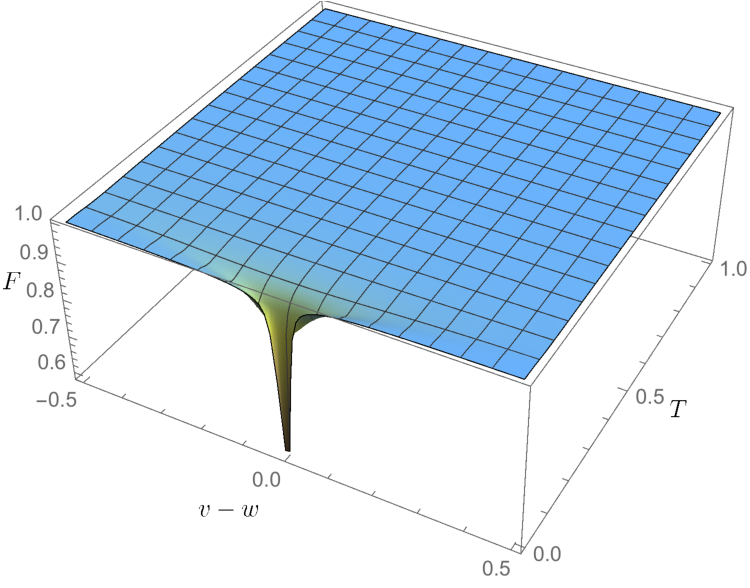
\includegraphics[width=0.7\textwidth,height=0.5\textwidth]{SSH_fidelity_theta.pdf}
\end{minipage}%
\begin{minipage}{0.33\textwidth}
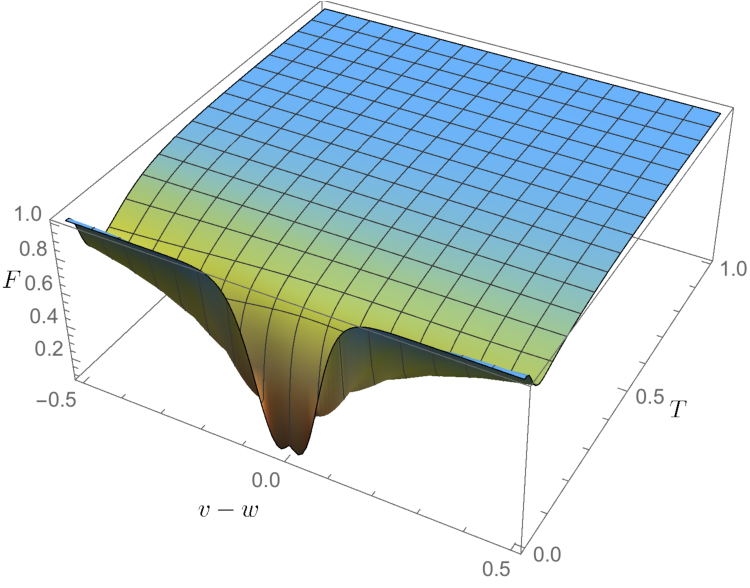
\includegraphics[width=0.7\textwidth,height=0.5\textwidth]{SSH_fidelity_T.pdf}
\end{minipage}
\begin{minipage}{0.33\textwidth}
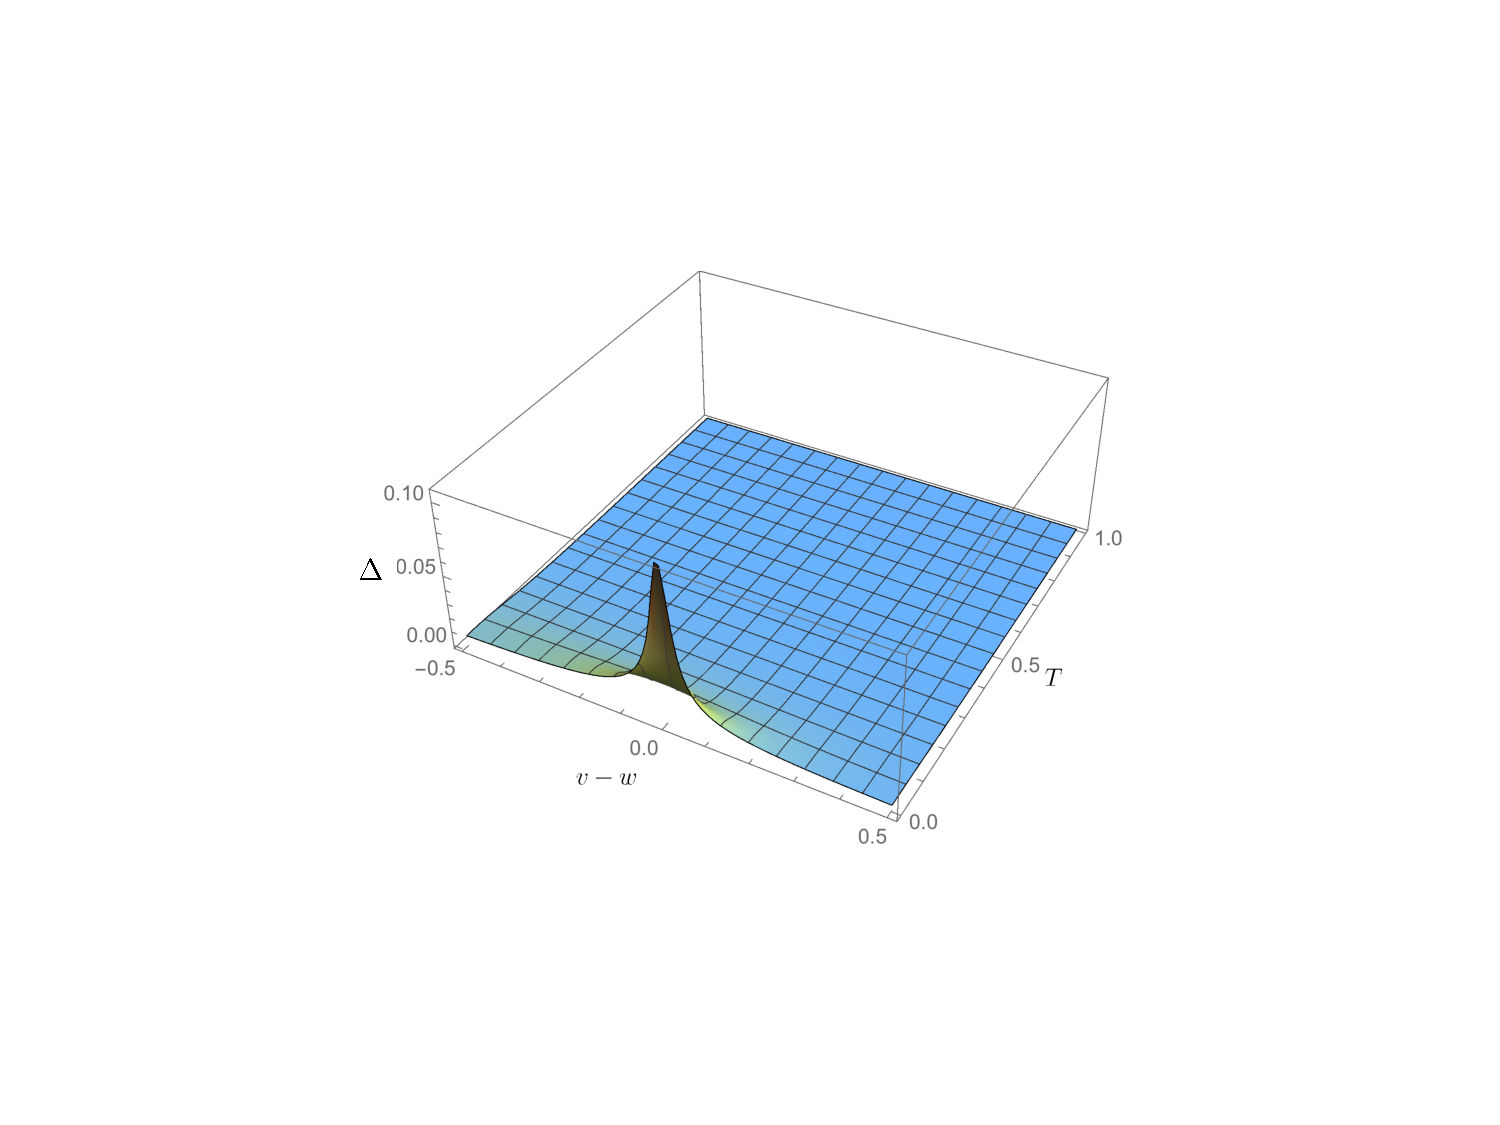
\includegraphics[width=0.7\textwidth,height=0.5\textwidth]{SSH_uhlmann_theta.pdf}
\end{minipage}%
\caption{The fidelity for thermal states $\rho$, when probing the parameter of the Hamiltonian that drives the topological PT $\delta |v-w| =|v-w|'-|v-w|=0.01$ (left), and the temperature $\delta T=T'-T=0.01$ (centre), and the Uhlmann connection, when probing the parameter of the Hamiltonian $|v-w|$ (right), for the TI SSH model (representative of the symmetry class BDI). The plot for $\Delta$ when $\delta |v-w|=0$ is omitted, since it is equal to zero everywhere.}
\label{fig:fid:ssh}
\end{figure}
The Hamiltonian for the TI Creutz Ladder model~\cite{cre:99,ber:pat:ami:del:09} is given by
\begin{eqnarray}
\mathcal{H}=& -\sum_{i\in\mathbb{Z}}K\left(e^{-i\phi}a_{i+1}^{\dagger}a_{i}+e^{i\phi}b_{i+1}^{\dagger}b_{i}\right)\nonumber\\
&+K(b_{i+1}^{\dagger}a_{i}+a_{i+1}^{\dagger}b_{i})+Ma_{i}^\dagger b_i +\text{H.c.},	
\end{eqnarray}
where $a_i,b_i$, with $i\in\mathbb{Z}$, are fermion annihilation operators, $K$ and $M$ are hopping amplitudes (horizontal/diagonal and vertical, respectively) and $e^{i\phi}$ is a phase factor associated to a discrete gauge field. We take $2K=1$, $\phi=\pi/2$. Under these conditions, the system is topologically nontrivial when $M<1$ and trivial when $M>1$. 
Similarly to the case of the SSH model, for two close points $(M,T)$ and $(M',T')=(M+\delta M, T+\delta T)$, we compute $F(\rho,\rho')$ and $\Delta(\rho,\rho')$ between $\rho=\rho(M,T)$ and $\rho'=\rho(M',T')$ and we consider the cases $\delta T = 0$ and $\delta M = 0$, respectively, see Figure~\ref{fig:fid:cl}.




\begin{figure}[h!]
\begin{minipage}{0.32\textwidth}
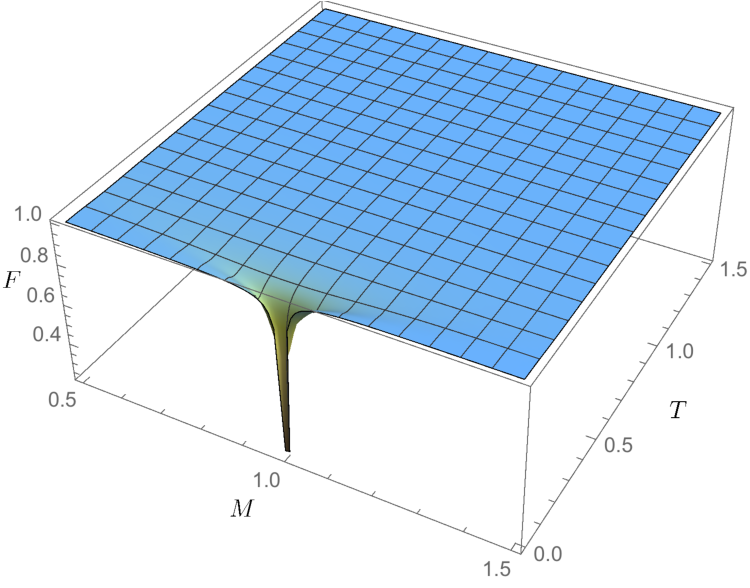
\includegraphics[width=0.7\textwidth,height=0.6\textwidth]{CL_fidelity_theta.pdf}
\end{minipage}
\begin{minipage}{0.32\textwidth}
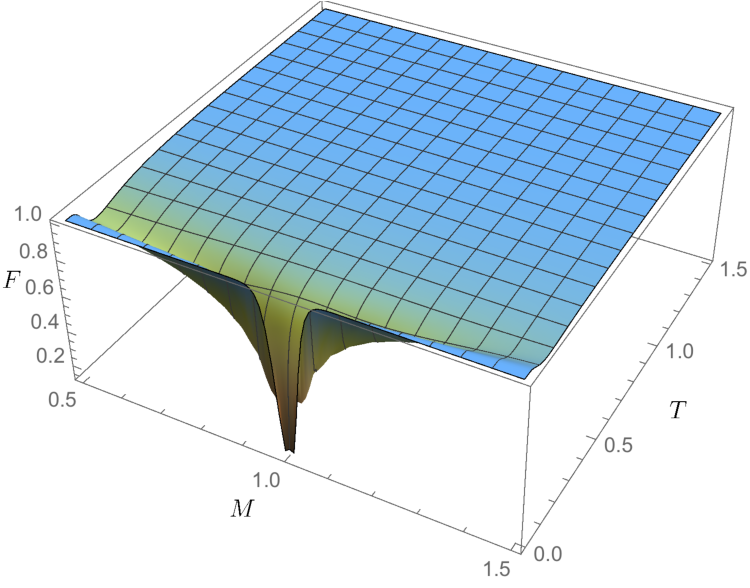
\includegraphics[width=0.7\textwidth,height=0.6\textwidth]{CL_fidelity_T.pdf}
\end{minipage}
\begin{minipage}{0.32\textwidth}
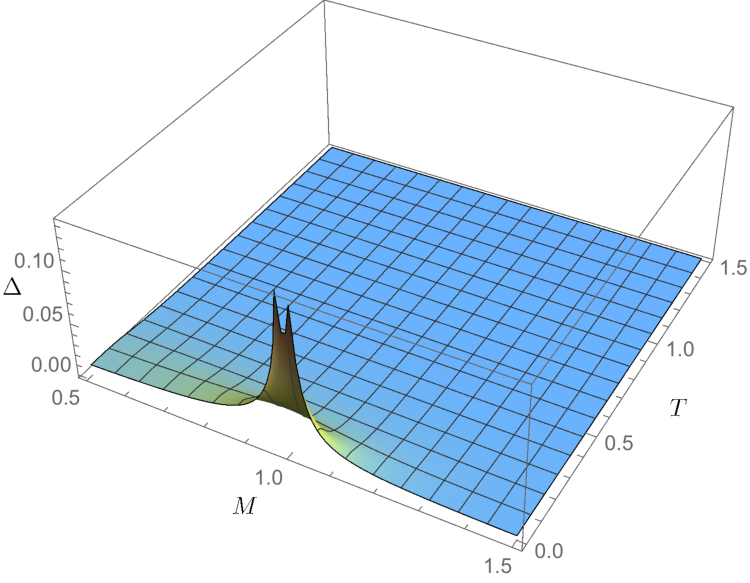
\includegraphics[width=0.7\textwidth,height=0.6\textwidth]{CL_uhlmann_theta.pdf}
\end{minipage}
\caption{The fidelity for thermal states $\rho$, when probing the parameter of the Hamiltonian that drives the topological PT $\delta M =M'-M=0.01$ (left), and the temperature $\delta T=T'-T=0.01$ (centre), and the Uhlmann connection, when probing the parameter of the Hamiltonian $M$ (right), for the TI Creutz ladder model (representative of the symmetry class AIII). The plot for $\Delta$ when deforming the thermal state along $T$ is omitted since it is equal to zero everywhere.}
\label{fig:fid:cl}
\end{figure}

Finally, we present our quantitative results for the TSC model. The Hamiltonian for the Kitaev Chain model~\cite{kit:cha:01} is given by
\begin{equation}
\mathcal{H}=-\mu\sum_{i=1}^N c^{\dagger}_i c_i+\sum_{i=1}^{N-1}\left[-t(c^{\dagger}_{i+1}c_i+c^{\dagger}_ic_{i+1})-|\Delta|(c_ic_{i+1}+c^{\dagger}_{i+1}c^{\dagger}_i)\right],
\end{equation}
 where $\mu$ is the chemical potential, $t$ is the hopping amplitude and $\Delta$ is the superconducting gap. 
 We fix $t=0.5,\Delta=1$, while the change of $\mu$ along the sites of the line drives the topological PT. In particular, the PT occurs at $\mu=1$ (gap closing point). Again, we calculate $F(\rho,\rho')$ and $\Delta(\rho,\rho')$ for $\rho=\rho(\mu,T)$ and $\rho'=\rho(\mu',T')$ for two close points $(\mu,T)$ and $(\mu',T')=(\mu+\delta \mu, T+\delta T)$ of the parameter space. In Figure~\ref{fig:fid:kit}, we show our results when probing the parameter of the Hamiltonian ($\delta T = 0$) and the temperature ($\delta \mu = 0$), separately.
  
 \begin{figure}[h!]
\begin{minipage}{0.33\textwidth}
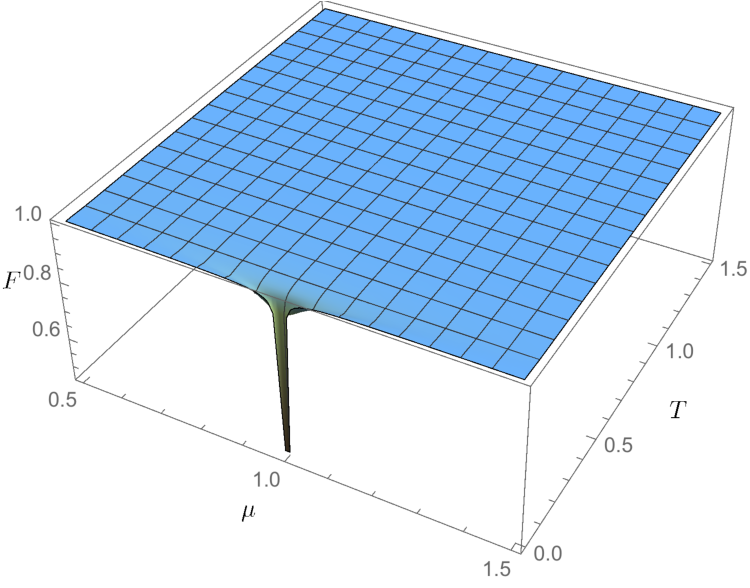
\includegraphics[width=0.7\textwidth,height=0.5\textwidth]{kitaev_fidelity_theta.pdf}
\end{minipage}%
\begin{minipage}{0.33\textwidth}
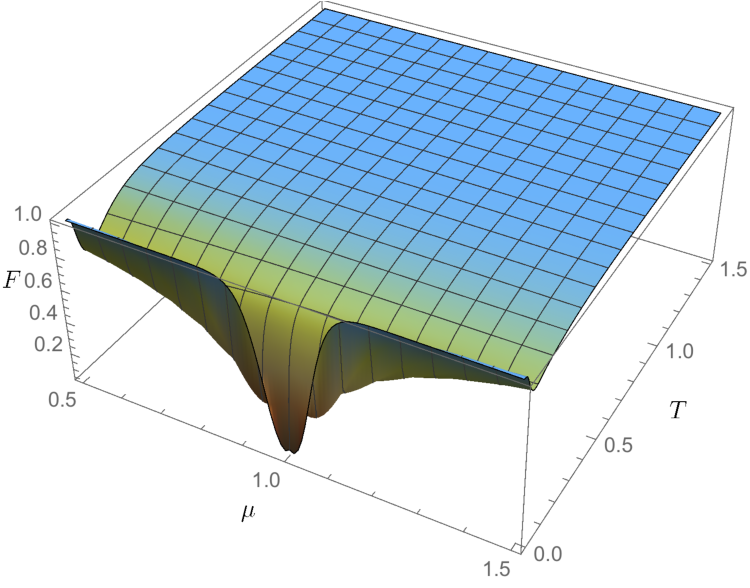
\includegraphics[width=0.7\textwidth,height=0.5\textwidth]{kitaev_fidelity_T.pdf}
\end{minipage}
\begin{minipage}{0.33\textwidth}
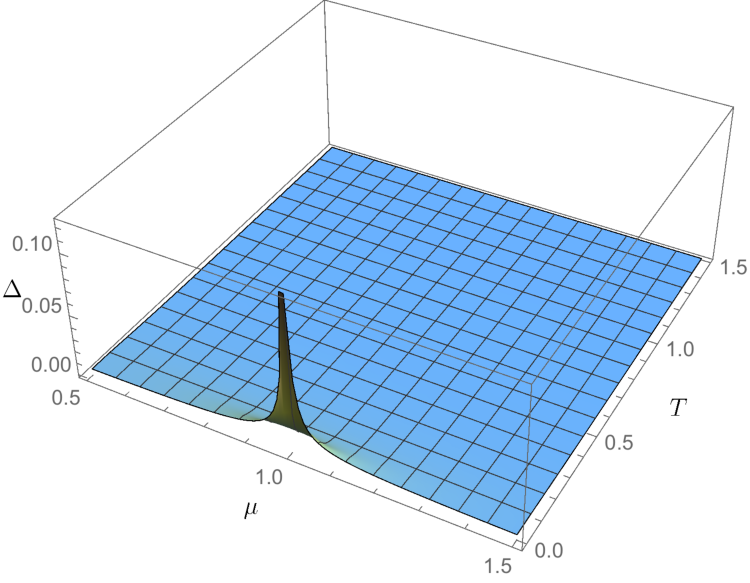
\includegraphics[width=0.7\textwidth,height=0.5\textwidth]{kitaev_uhlmann_theta.pdf}
\end{minipage}%
\caption{The fidelity for thermal states $\rho$, when probing the parameter of the Hamiltonian that drives the topological PT $\delta \mu =\mu'-\mu=0.01$ (left), and the temperature $\delta T=T'-T=0.01$ (centre), and the Uhlmann connection, when probing the parameter of the Hamiltonian $\mu$ (right), for the TSC Kitaev chain model. The plot for $\Delta$ when $\delta \mu=0$, is trivial (equal to zero everywhere), thus we omit it.}
\label{fig:fid:kit}
\end{figure}

For all the three cases that we presented the behaviour of the fidelity and the quantity $\Delta$ is qualitatively the same.
We see that for $T=0$ the fidelity exhibits a sudden drop in the neighbourhood of the gap-closing points, signalling the topological quantum PTs. As temperature increases, the drop of fidelity at the quantum critical points is rapidly smoothened towards the $F=1$ value. This shows the absence of both finite-temperature parameter-driven, as well as temperature-driven (i.e., thermal) PTs. The plots of $\Delta$ for $\delta T=0$, show a behaviour similar to that of the fidelity, while if we only change the temperature and not the parameter of the Hamiltonian, we obtain no information, as $\Delta$ is identically equal to zero, due to the triviality of the Uhlmann connection associated to the mutually commuting states (a consequence of the Hamiltonian's independence on the temperature). $\Delta$ is sensitive to PTs for which the state change is accompanied by a change of the eigenbasis (in contrast to fidelity, which is sensitive to both changes of eigenvalues and eigenvectors). For TIs and TSCs, this corresponds to parameter-driven transitions only. 
\section{Edge states of topological insulators and superconductors}
\label{sec:edge}
When one considers topological systems on a finite-size chain with open boundary conditions, the bulk-to-boundary correspondence principle~\cite{x:g:wen:91,ryu:hat:02} predicts the existence of zero modes localised at the ends of the chain, whenever the bulk is in a topologically non-trivial phase. It is then possible to consider the associated thermal states, $\rho=\exp(-\beta \mathcal{H})/Z$, and probe the effects of temperature. The study of the Uhlmann connection and the fidelity conducted in the previous section suggests that at zero temperature the edge states should exhibit an abrupt change as the system passes the point of quantum phase transition, while at finite temperatures they should smoothly change, slowly being washed away with the temperature increase, as a consequence of the absence of finite-temperature transitions. Below, we first study TIs in Section~\ref{sec:edgeTI}, while in Section~\ref{sec:edgeTSC} we analyse a TSC given by the Kitaev model, showing the agreement with the above inferred behaviour.

\subsection{Topological insulators}
\label{sec:edgeTI}
 Let us consider the Creutz ladder model as a representative of TIs. Similar results are obtained when considering the SSH model and we omit them for the sake of briefness. In the trivial phase, the spectrum decomposes into two bands of states separated by a gap. At zero chemical potential, the zero-temperature limit of $\rho$ is the projector onto the Fermi sea state $\ket{\text{FS}},$ obtained by occupying the lower band. On a topologically non-trivial phase, however, the spectrum is composed of the two bands {\em and} the zero modes. At zero chemical potential, the zero temperature limit of $\rho$ is now the projector onto the ground state manifold of $\mathcal{H}$, which is spanned by $\ket{\text{FS}}$ and additional linearly independent states by creating excitations associated to the zero modes. Since the Fermi sea does not have these edge state excitations (exponentially localised at the boundary) included, the occupation number as a function of position, $n_i=a_i^\dagger a_i+b_i^{\dagger}b_i$, will see this effect at the boundary of the chain. Indeed, this is what we see in Figure~\ref{fig:FS_occupation_number}: the occupation number, as a function of position, drops significantly at the edges in the topologically non-trivial phase. On the other hand, on the topologically trivial side the occupation number stays constant throughout the whole chain (both bulk and the edges).



\begin{figure}[h!]
\begin{minipage}{0.45\textwidth}
\centering
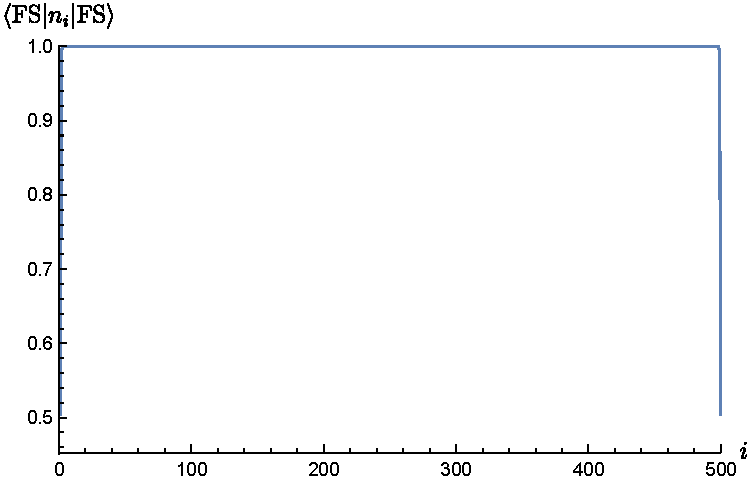
\includegraphics[scale=0.5]{fermisea_topological.pdf}
\end{minipage}
\begin{minipage}{0.45\textwidth}
\centering
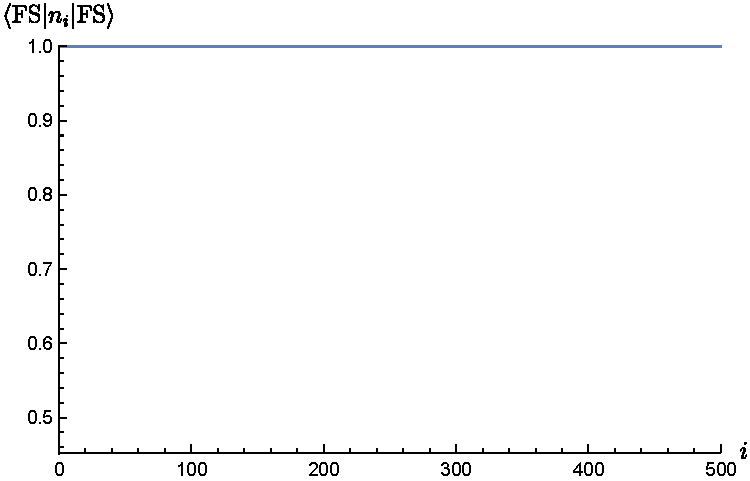
\includegraphics[scale=0.5]{fermisea_trivial.pdf}
\end{minipage}
\caption{Fermi sea expectation value of the occupation number $n_i=a_i^\dagger a_i+b_i^{\dagger}b_i$ as a function of position $i$ on a chain of 500 sites with open boundary conditions for a TI (Creutz ladder model). On the left panel the system is in a topologically non-trivial phase with $2K=1,M=0.1,\phi=\pi/2$. On the right panel the system is in a topologically trivial phase with $2K=1,M=1.0001,\phi=\pi/2$.}
\label{fig:FS_occupation_number}
\end{figure}



If we want the thermal state's $T=0$ limit to be the Fermi sea, we have to add a very small (negative) chemical potential. It has to be small enough so that the lower band gets completely filled. In the following Figure~\ref{fig:BG_occupation_number}, we see that the expectation value $\tr(\rho n_i)$ coincides with $\bra{\text{FS}}n_i\ket{\text{FS}}$ in the $T=0$ limit and the deviation of the occupation number at the edge from that in the bulk gets washed out smoothly as the temperature increases. In fact, in the large temperature limit, the state is totally mixed, implying that the expected value of the occupation number will be constant and equal to $1$, as a function of position.  

\begin{figure}[h!]
\begin{minipage}{0.45\textwidth}
\centering
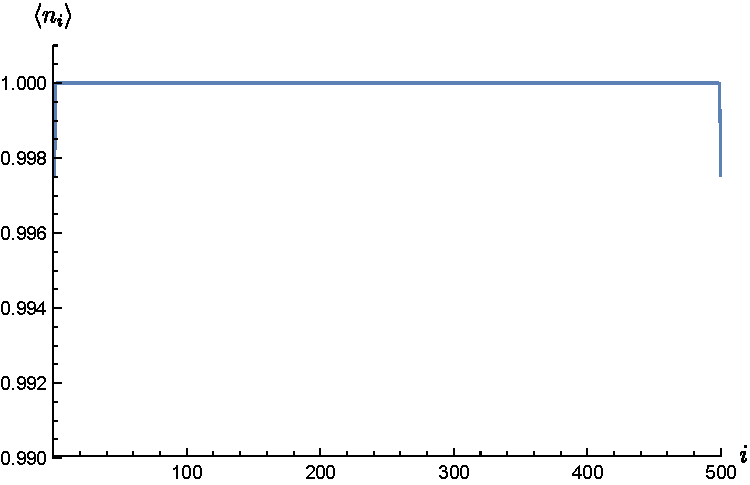
\includegraphics[scale=0.55]{occupation_T_100.pdf}
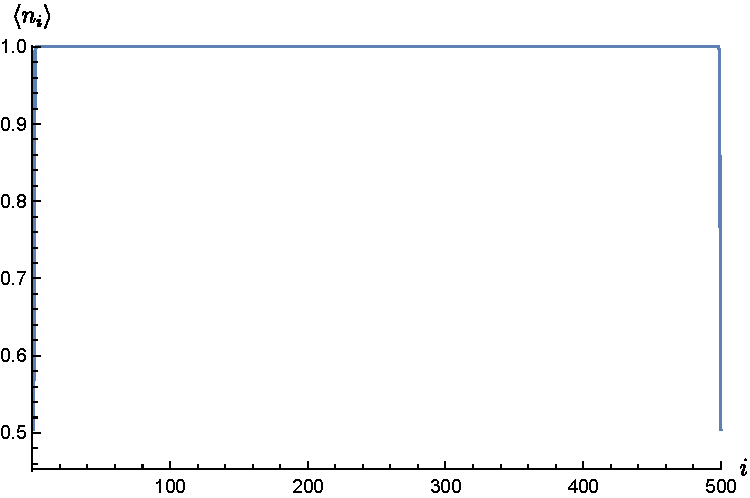
\includegraphics[scale=0.55]{occupation_zero_T.pdf}
\end{minipage}
\begin{minipage}{0.45\textwidth}
\centering
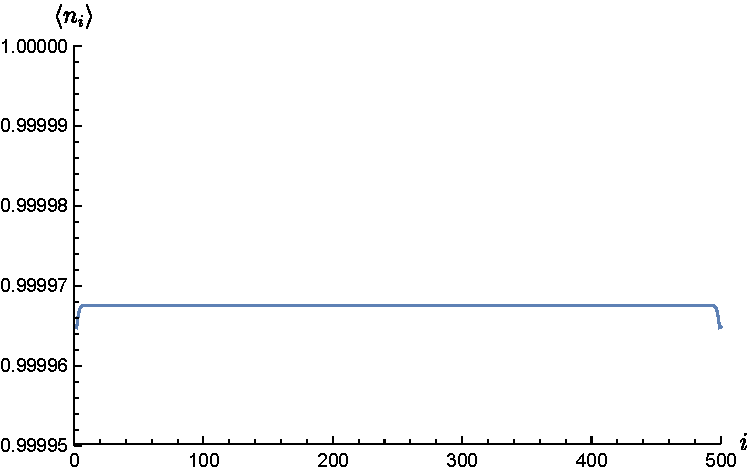
\includegraphics[scale=0.55]{occupation_finite_T_trivial.pdf}
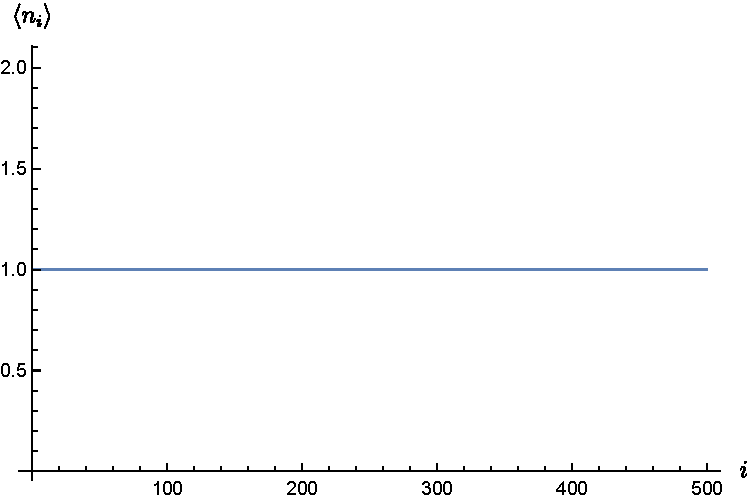
\includegraphics[scale=0.55]{occupation_zero_T_trivial.pdf}
\end{minipage}
\caption{Expectation value of the occupation number $n_i=a_i^\dagger a_i+b_i^{\dagger}b_i$ as a function of position $i$ on a chain of 500 sites with open boundary conditions for a TI (Creutz ladder model). In the left panel, we show the topologically non-trivial phase with $2K=1,M=0.1,\phi=\pi/2$, for temperatures $T=10^{-5}$ (down) and $T=0.2$ (up). On the right panel we have a topologically trivial phase near the critical value of the parameter $2K=1,M=1.0001,\phi=\pi/2$, for temperatures $T=10^{-5}$ (down) and $T=0.2$ (up). Increasing $M$, the edge behaviour is washed out smoothly, for finite $T$, and it becomes trivial as for the $T=0$ case.}
\label{fig:BG_occupation_number}
\end{figure}
We see that the results presented in Figures~\ref{fig:FS_occupation_number} and~\ref{fig:BG_occupation_number} confirm the results obtained by the fidelity analysis and the study of the Uhlmann connection in terms of the quantity $\Delta$. Indeed, the fact that the edge states localised at the boundary between two distinct topological phases, that manifest the topological order at zero temperature, are gradually smeared out as we increase the temperature, confirm the absence of finite-temperature PTs. Furthermore, our results on the edge states, obtained for systems in thermal equilibrium, agree with those concerning open systems treated within the Lindbladian approach~\cite{viy:riv:del:12} (and consequently, due to considerable computational hardness, obtained for an open chain of only 8 sites).

\subsection{Topological superconductors}
\label{sec:edgeTSC}
 As far as the TSC Kitaev model is concerned, the chemical potential is a parameter of the Hamiltonian and we cannot lift the zero modes from the zero-temperature limit of $\rho$ with the above method. Moreover, the Kitaev Hamiltonian does not conserve the particle number, and adding chemical potential associated to the total particle number would not lift the zero modes even if $\mu$ were not a parameter of the Hamiltonian.  Note though, that the total number of Bogoliubov {\em quasi-particles} which diagonalise the Hamiltonian is conserved. Hence, we add a very small (negative) chemical potential associated with the total quasi-particle number, thereby lifting the Majorana zero modes energy.  We found that the good quantity to be studied is not the occupation number as a function of the position in the chain, but the ratio between the average particle occupation number at the edge and the average particle occupation number at the bulk $f(\mu;T) = \langle n_{\text{edge}}\rangle/\langle n_{\text{bulk}}\rangle$ (without loss of generality, we have chosen for $n_{\text{bulk}}$ the site in the middle of the chain, since it is approximately constant throughout the bulk). 
 In Figure~\ref{fig:majorana}, we present the results obtained for a chain with open boundary conditions, consisting of 300 sites.
 
 
 \begin{figure}[h!]

\centering
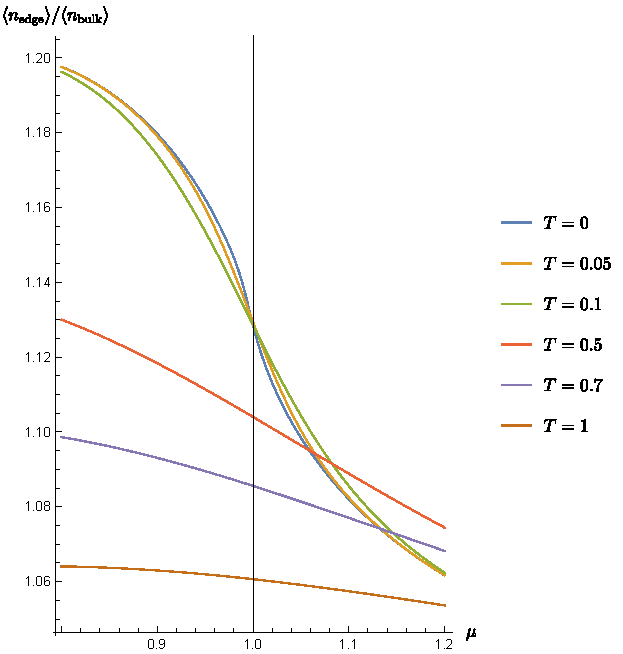
\includegraphics[scale=0.6]{majorana_paper_plot.pdf}

\caption{$\langle n_{\text{edge}}\rangle/\langle n_{\text{bulk}}\rangle$ as a function of the chemical potential $\mu$ for a chain of 300 sites with open boundary conditions, for several values of the temperature $T$.}
\label{fig:majorana}
\end{figure}

The results are consistent with the behaviour inferred by the Uhlmann connection and the fidelity: Majorana modes exhibit an abrupt change at zero temperature (a signature of the quantum PT), while for fixed finite temperatures they smoothly change with the parameter change, and are slowly washed away with the temperature increase. Indeed, the behaviour of the finite-temperature curves is smooth, while the zero-temperature quench-like curve is expected to develop a discontinuity at $\mu = 1$ in the thermodynamic limit (see for example Fig.4(b) and the respective discussion in~\cite{qua:zur:10}). To show this more accurately, one needs considerably higher computational power to probe chain lengths of much higher orders of magnitude, a relevant future direction of work. 

The behaviour of the edge states and the associated Majorana modes reveals an interesting property of these systems which, at finite temperatures, despite the absence of phase transitions, they keep exhibiting their topological features even on the ``trivial side'' of the phase diagram (for parameter values for which on zero temperature the system is topologically trivial). At zero temperature, the Majorana modes are known to be good candidates for qubit encoding, see~\cite{ali:12,ipp:riz:gio:maz:16,majorana:17,majorana:twist:17} and references therein. Therefore, the aforementioned property of Majorana modes at the low but finite-temperature regime, is potentially significant in constructing realistic quantum memories. Furthermore, the existence of stable quantum memories has considerable impact in cryptography~\cite{rod:mat:pau:sou:17,pir:ott:spe:wee:bra:llo:geh:jac:and:15,ber:chr:col:ren:ren:10,dam:feh:ren:sal:sch:07,weh:sch:ter:08,sch:ter:weh:09,ng:jos:che:kur:weh:12,koe:weh:wul:12,bou:feh:gon:sch:13,lou:alm:and:pin:mat:pau:14}, as explained in Chapter~1.

Finally, we should stress that this new method to study Majorana modes is more general and also applicable to TIs: since the Hamiltonian conserves the total particle number, and the quasi-particle creation operators are linear combinations of {\em just} the particle creation operators (and not of the holes as well), the total quasi-particle and particle numbers coincide in this case. The results obtained for TIs using this new method lead to the same qualitative conclusion regarding the behaviour of the edge states (consistent with our previous results) and we omit them in order to avoid repetition.


\section{Fidelity and $\Delta$ analysis of BCS superconductors}
\label{sec:bcs}
In this section we study a topologically trivial superconducting system, as described by the BCS theory~\cite{bar:coo:sch:57}, with the effective Hamiltonian 
\begin{eqnarray}
\label{eq:BCS_MF}
\mathcal{H}=\sum_{k} (\varepsilon_{k}-\mu)c_{k}^{\dagger}c_{k}-\Delta_{k} c_{k}^{\dagger}c_{-k}^{\dagger} + \text{H.c.},
\end{eqnarray}
where $\varepsilon_k$ is the energy spectrum, $\mu$ is the chemical potential, $\Delta_{k}$ is the superconducting gap, $c_{k}\equiv c_{k\uparrow}$ and $c_{-k}\equiv c_{-k \downarrow}$ are operators annihilating an electron with momentum $k$ and spin up and an electron with momentum $-k$ and spin down, respectively. The gap parameter is determined in the above mean-field Hamiltonian through a self-consistent mass gap equation and it depends on the original Hamiltonian's coupling associated to the lattice-mediated pairing interaction $V,$ absorbed in $\Delta_k$ (for more details, see~\cite{pau:vie:08}). The solution of the equation renders the gap temperature-dependent.
In Figure~\ref{fig:bcs}, we show the quantitative results for the fidelity and $\Delta$. 
\begin{figure}[h!]
\begin{minipage}{0.24\textwidth}
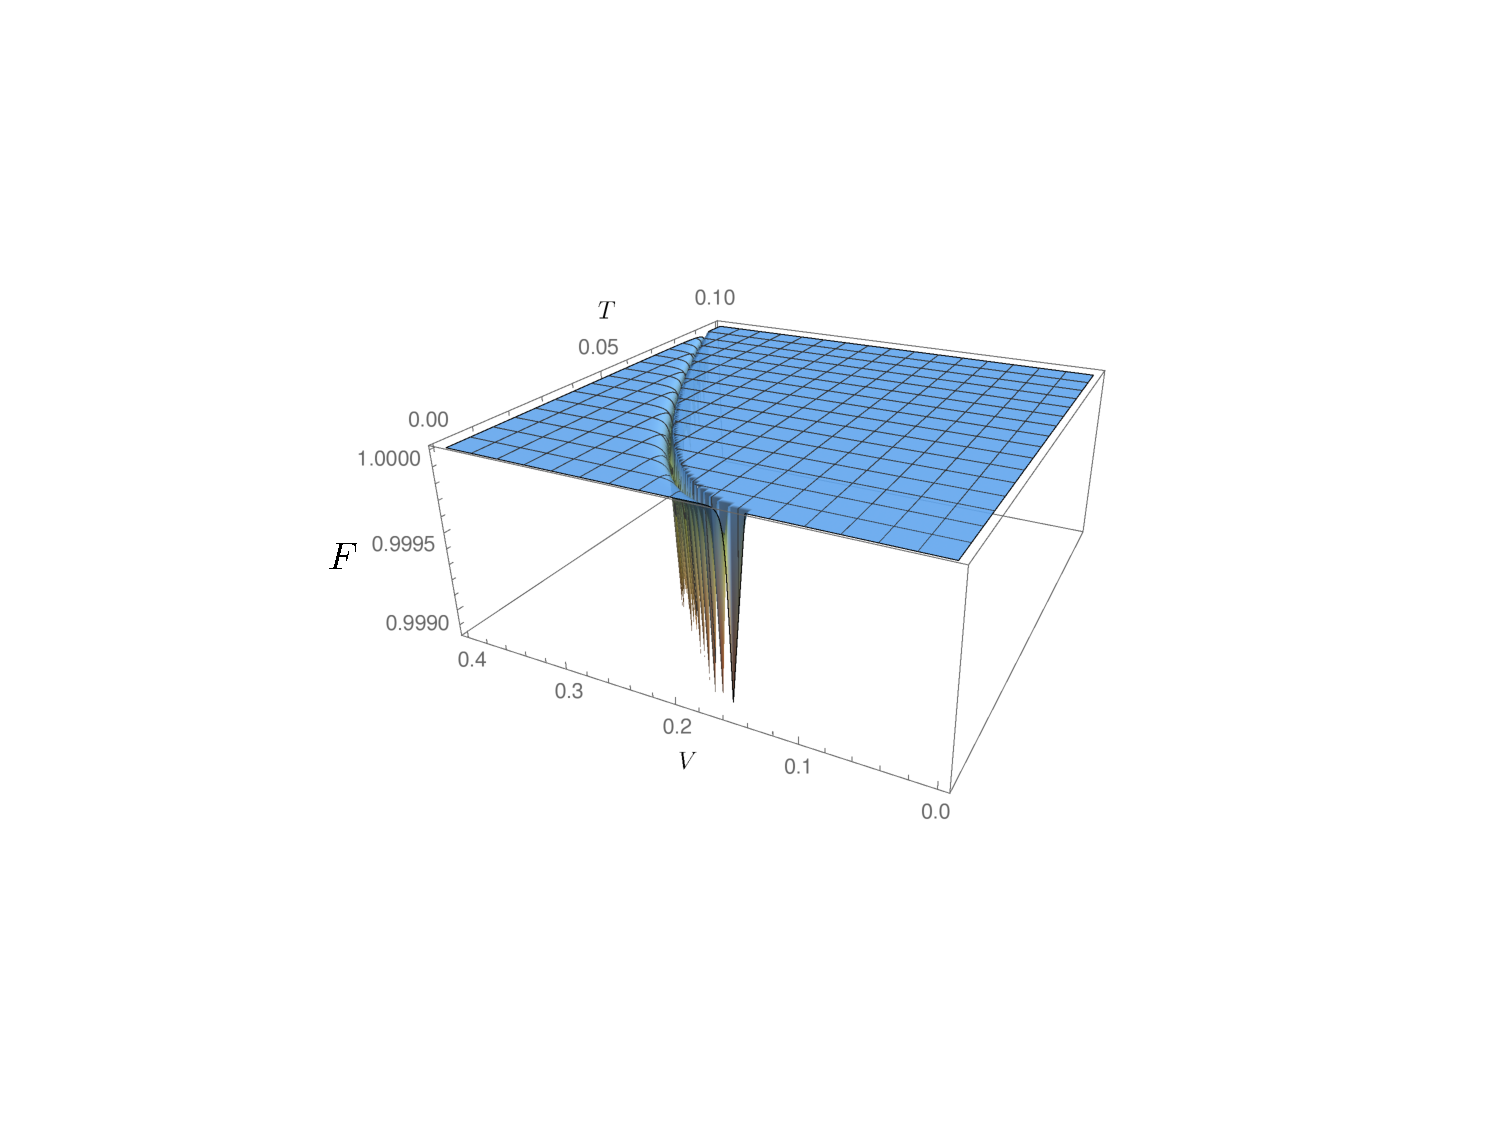
\includegraphics[width=0.8\textwidth,height=0.6\textwidth]{BCS_fidelity_theta.pdf}
\end{minipage}%
\begin{minipage}{0.24\textwidth}
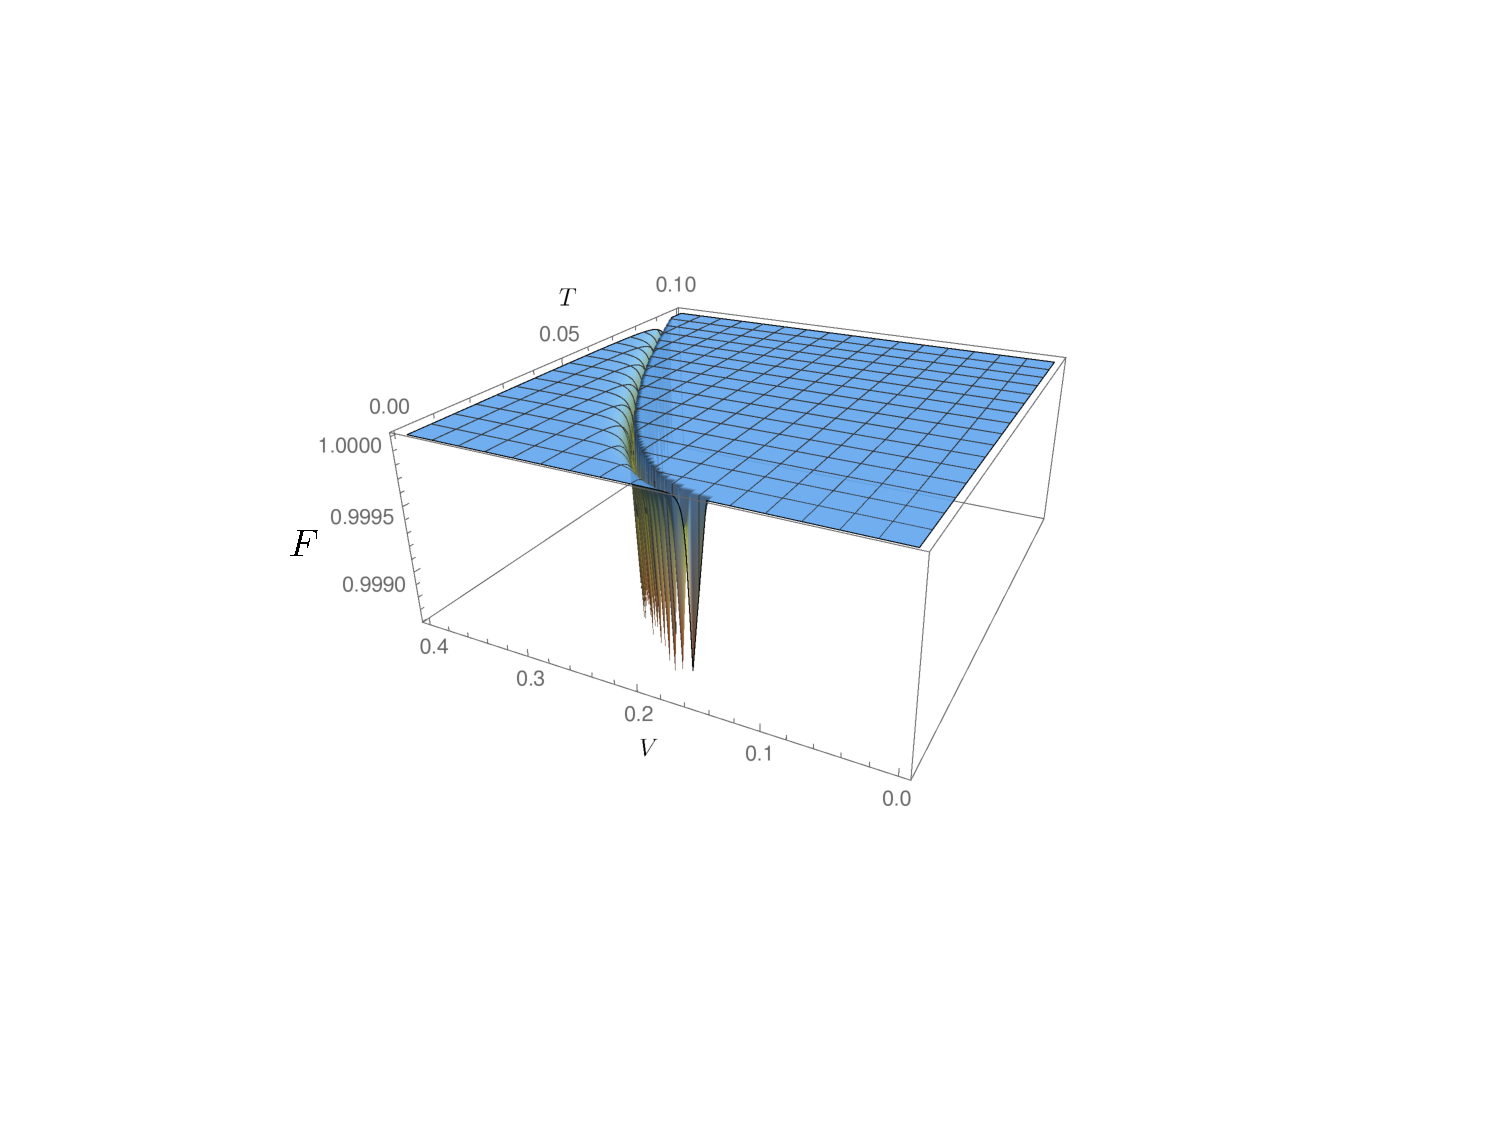
\includegraphics[width=0.8\textwidth,height=0.6\textwidth]{BCS_fidelity_T.pdf}
\end{minipage}
\begin{minipage}{0.24\textwidth}
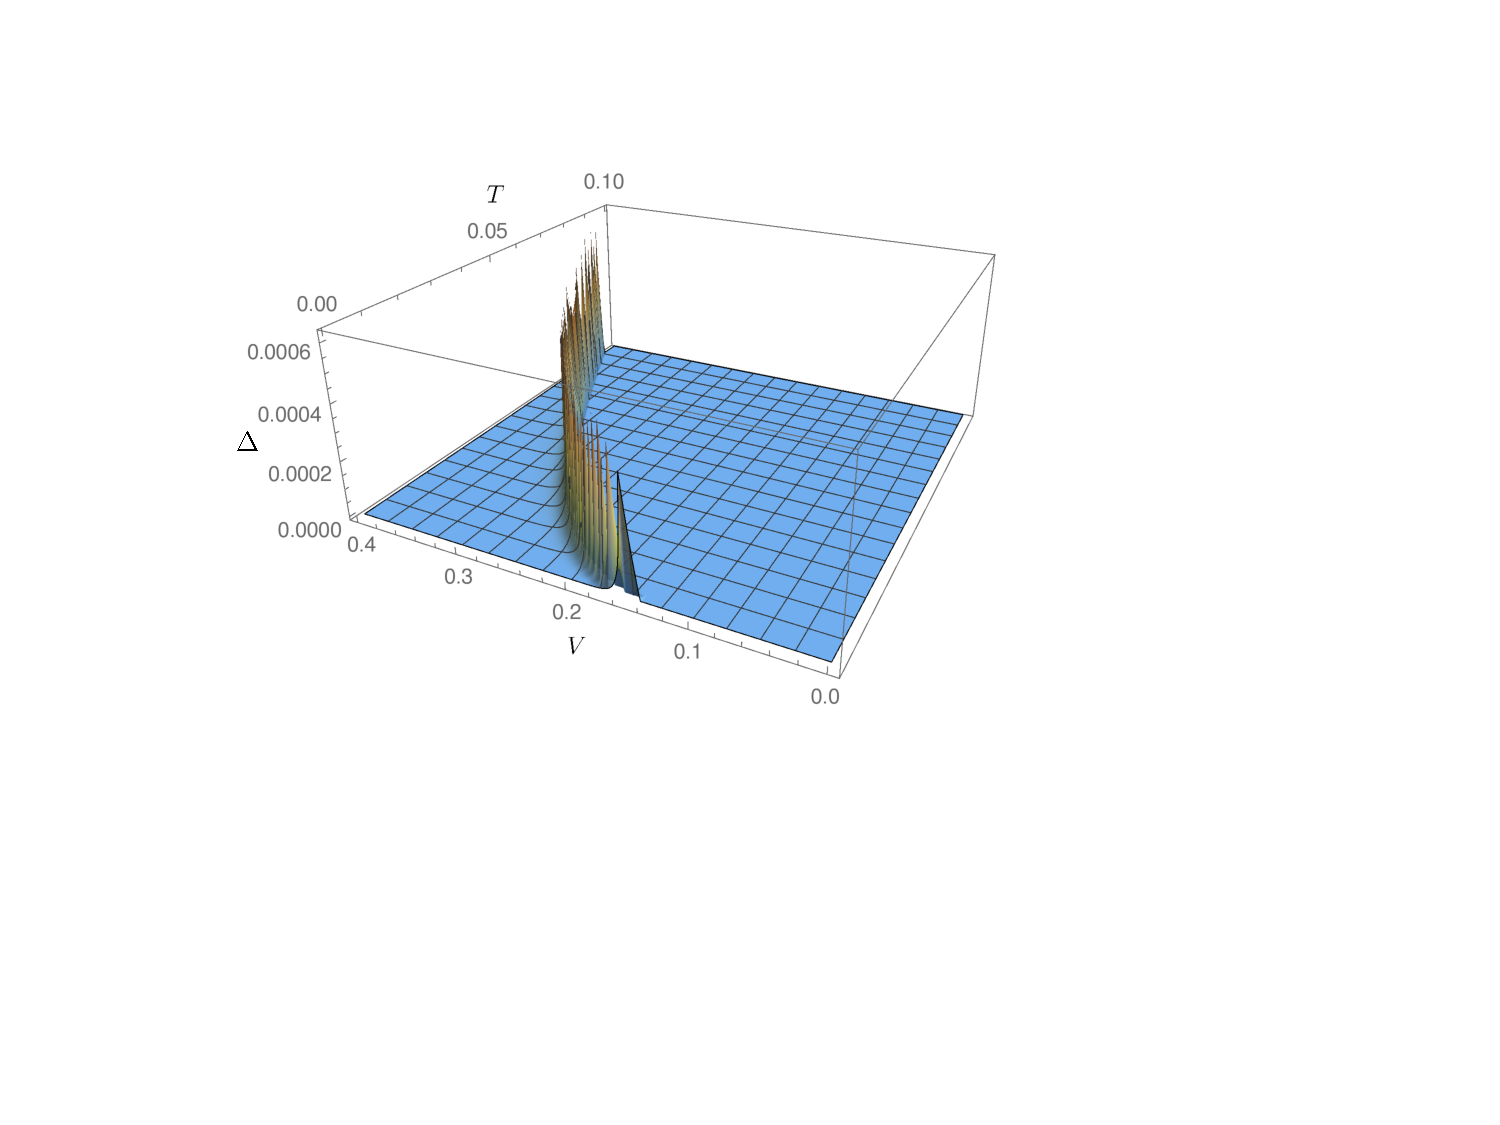
\includegraphics[width=0.8\textwidth,height=0.6\textwidth]{BCS_delta_theta.pdf}
\end{minipage}%
\begin{minipage}{0.24\textwidth}
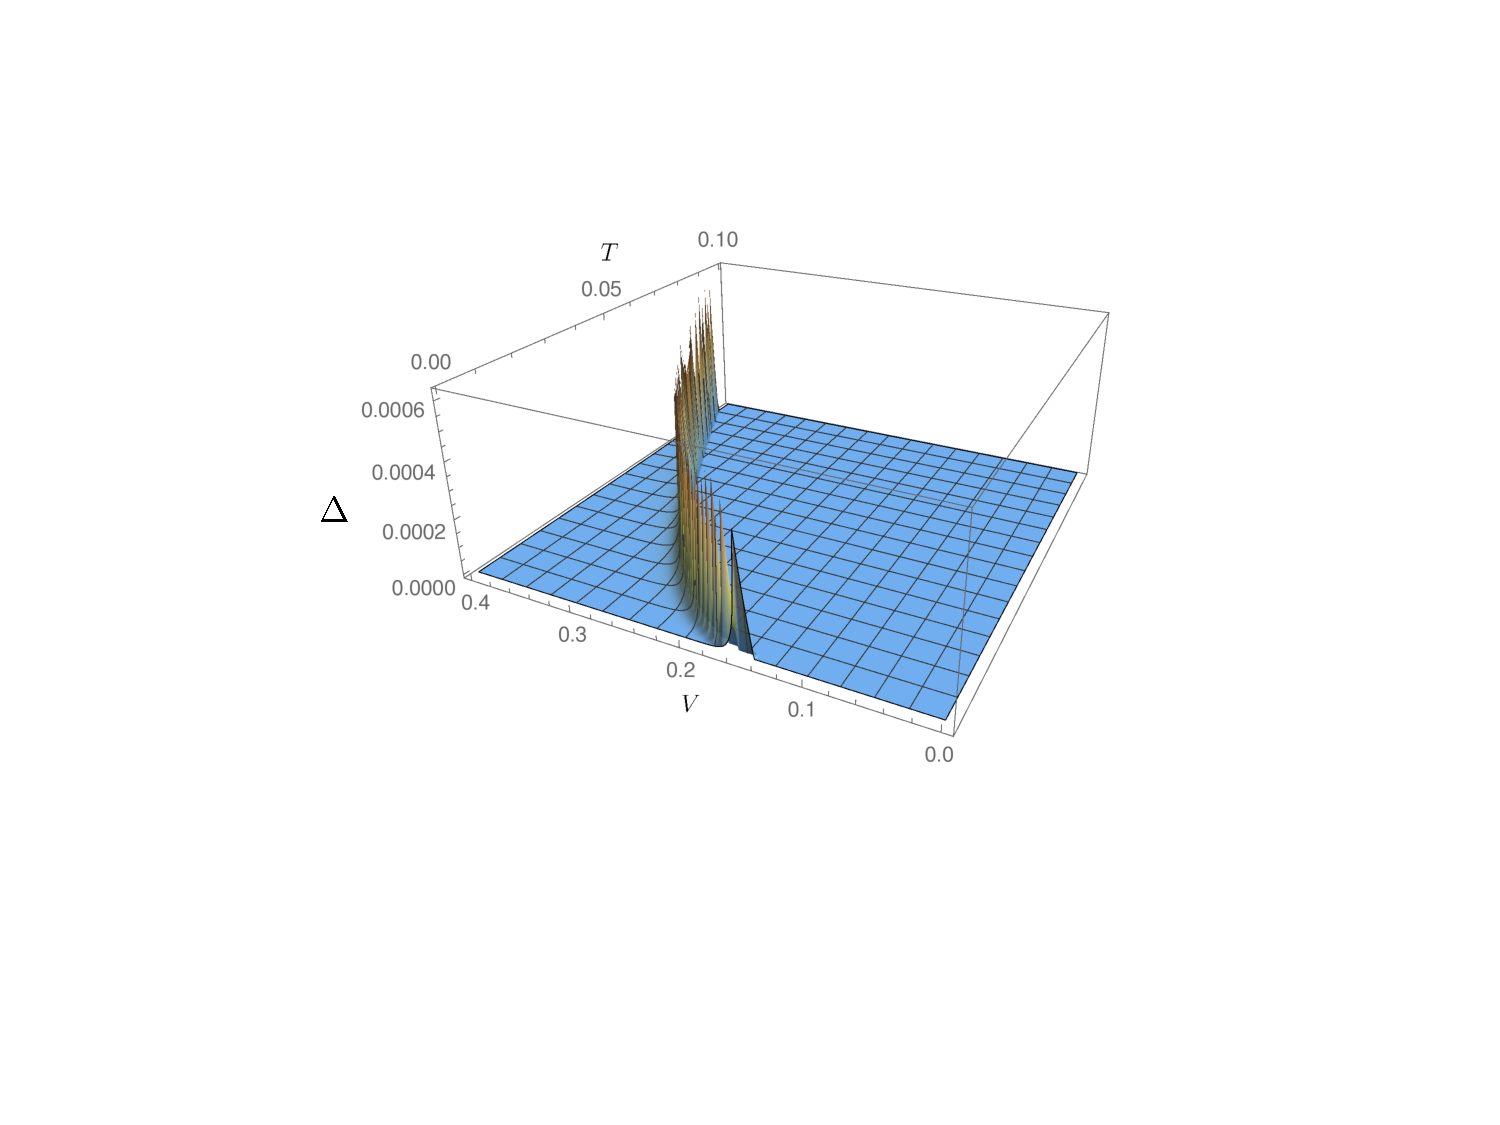
\includegraphics[width=0.8\textwidth,height=0.6\textwidth]{BCS_delta_T.pdf}
\end{minipage}
\caption{The fidelity for thermal states $\rho$ when probing the parameter of the Hamiltonian $\delta V =V'-V=10^{-3}$ (left) and the temperature $\delta T=T'-T=10^{-3}$ (centre left), and the Uhlmann connection (centre right and right, respectively), for BCS superconductivity.}
\label{fig:bcs}
\end{figure}
We observe that both quantities show the existence of thermally driven PTs, as their abrupt change in the point of criticality at $T=0$, survive and drift, as temperature increases. This behaviour is in sharp contrast to the respective behaviour of the topologically non-trivial systems, for which there exist no finite-temperature PTs.

It is interesting to compare the two cases of superconductors studied, and try to isolate the reasons for such difference. 
Unlike TSCs, in the BCS model the temperature does not only appear in the thermal state, but it is also a parameter of the effective Hamiltonian (recall that the superconducting gap depends on temperature), resulting in the change of the system's eigenbasis and consequently a non-trivial Uhlmann connection. In particular, the quantity $\Delta$, which quantifies the rate of change of the system's eigenbasis, reflects the quantum contribution to the state distinguishability (see also~\cite{zan:ven:gio:07}, equation (3), in which the Bures metric is split into classical and non-classical terms, the first quantifying the change of system's eigenvalues and the second the change of the corresponding eigenvectors). Thus, the Uhlmann connection is trivial in the cases of the topological systems considered, as their Hamiltonians do not explicitly depend on temperature and thus commute with each other at finite temperatures. On the other hand, the mean-field BCS Hamiltonian considered does explicitly depend on the temperature, and as the results presented above clearly show, the change of the eigenbasis of the BCS thermal states carries the signature of a thermally driven PT. Note that, having a purely non-classical contribution, such a temperature-driven PT has quantum features as well, which is on its own an interesting consequence of the study of the Uhlmann connection.

To illustrate this difference between TSCs and BCS better, let us explain the above with a few more details.
In the case of the BCS superconductivity we considered the effective mean-field Hamiltonian given by Equation~\eqref{eq:BCS_MF},
in which the gap $\Delta(V,T)$ is a function of temperature. Had we considered a more fundamental ``pairing Hamiltonian'', which takes into account the quartic electron interaction mediated by the phonons of the lattice,
\begin{equation}
\label{eq:BCS_P}
\mathcal{H}^{P}=\sum_{k} (\varepsilon_{k}-\mu)c_{k}^{\dagger}c_{k}-\sum_{k,k'} V_{k,k'}c_{k'}^{\dagger}c_{-k'}^{\dagger}c_{-k}c_{k} + \text{H.c.},	
\end{equation}
the Uhlmann connection would be trivial. The mean-field Hamiltonian of Equation~\eqref{eq:BCS_MF} is obtained from Equation~\eqref{eq:BCS_P} by means of the BCS decoupling scheme with an averaging procedure, setting the effective gap for the mean-field state $\rho = e^{-\beta\mathcal{H}}/Z$ (for simplicity, we assume $V_{kk'} = -V$ for $k,k'$ close to the Fermi momentum $k_F$, and zero otherwise) to be
\begin{equation}
\label{eq:gap}
\Delta(V,T) = -\sum_{k'} V_{kk'} \langle c_{-k}c_{k}\rangle = V \sum_k \mbox{Tr}(c_{-k}c_{k}\rho ).	
\end{equation}

In other words, the effective mean-field Hamiltonian of Equation~\eqref{eq:BCS_MF} is obtained from Equation~\eqref{eq:BCS_P} by expanding $c_{-k}c_{k} = \langle c_{-k}c_{k}\rangle + \delta(c_{-k}c_{k})$ around the suitably chosen superconducting ground state. Thus, $\mathcal{H}$ breaks the $\mbox{U}(1)-$~particle-number conservation symmetry of $\mathcal{H}^P$ to a residual $\mathbb Z_2$ symmetry, in order to accommodate the superconducting properties of the system. As a result, the Uhlmann connection becomes sensitive to temperature-driven PTs, due to the enhanced state distinguishability in terms of the system's eigenbasis. On the other hand, the Hamiltonian of the Kitaev model is phenomenological, modelled upon the success of the related BCS mean-field Hamiltonian. In this model, the gap is, for simplicity, considered to be temperature-independent. One might thus question whether the gap of a general superconducting material should also a priori depend on the temperature. It would be interesting to probe this  in experiments with realistic topological superconducting materials. Our method based on the Uhlmann connection could then be particularly useful in the analysis of such experiments.

\section{The choice of the parameter space in the study of topological phase transitions}
\label{sec:space}
We will conclude this chapter, by commenting on the relevance of the choice of the parameter space in the study of PTs in topologically ordered systems.
In order for the Uhlmann connection and the fidelity to be in tune, they must be taken over the same base space, which in our study consists of the parameters of the Hamiltonian and the temperature. In a previous study~\cite{viy:riv:del:14}, the Uhlmann connection for 1D topologically ordered systems was considered in the momentum space and with respect to single-particle density matrices of the form $\{\rho_k:=e^{-\beta H_k}/Z: k\in \mathcal B \}$. In order to infer the possibility of finite-temperature PTs, the authors used the Uhlmann geometric phase $\Phi_U(\gamma_c)$ along the closed curve $\gamma_c(k)=\rho_k$, given as 
\[
\Phi_U(\gamma_c)=\arg\tr\{w(-\pi)^{\dagger}w(\pi)\} =\arg\tr\{\rho_{\pi}U(\gamma_c)\},
\]
where $w(k)$ is the horizontal lift of the loop of density matrices $\rho_{k}$, and $U(\gamma_c)$ is the so-called Uhlmann holonomy obtained by imposing the Uhlmann parallel transport condition along the first Brillouin zone $\mathcal B$.
It was found that $\Phi_U(\gamma_c)$ changes abruptly from $\pi$ to $0$ after some ``critical'' temperature $T_U$. The authors identified this abrupt change of $\Phi_U(\gamma_c)$, as a finite-temperature topological PT ``in the Uhlmann sense'', in analogy to the pure-state case, where the abrupt change of the Berry phase signals a topological PT~\cite{ber:84}. Note, also, that the zero-temperature limit of the Uhlmann geometric phase is the Berry phase. However, for the topological systems studied in~\cite{viy:riv:del:14}, the Uhlmann holonomy is a smooth function of the temperature and is given, in the basis in which the CS operator is diagonal, by:
\label{eq:hol}
\[
U(\gamma_c) = \exp \Big\{-\frac{i}{2} \int_{-\pi}^{\pi} \left[1 - \text{sech} \left(\frac{E_k}{2T}\right)\right]\frac{\partial \varphi_k}{\partial k}dk\  \sigma_z\Big\},
\]
where $\varphi_k$ is the polar angle coordinate of the vector $\vec{n}_k$ lying on the equator of the Bloch sphere.  So, while the Uhlmann phase suffers from an abrupt change, the Uhlmann holonomy is smooth, hence there is no PT-like behaviour. Conversely, there might be cases, where the Uhlmann phase is trivial, $\Phi_U(\gamma_c) = 0$, while the corresponding holonomy is not, $U(\gamma_c)\neq I$.
Moreover, the associated critical temperature is not necessarily related to a physical quantity that characterises a system's phase.\\

In the paradigmatic case of the quantum Hall effect~\cite{and:mat:uem:75}, at $T=0$, the Hall conductivity is quantised in multiples of the first Chern number of a vector bundle in momentum space through several methods. For example, one can use linear response theory or integrate the fermions to obtain the effective action of an external $\text{U}(1)-$~gauge field. The band topology appears, thus, in the response of the system to an external field. In this context, it is unclear how the Uhlmann geometric phase along the cycle of the 1D momentum space, can have an interpretation in terms of the physical response of the system. In order to measure it, one would have to be able to change the quasi-momentum of a state in an adiabatic way. In realistic setups, the states at finite temperatures are statistical mixtures over all momenta, such as the thermal states considered, and realising closed curves of states $\rho_k$ with precise momenta changing in an adiabatic way seems to be a tricky task. The fidelity computed in our work though, refers to the change of the system's {\em overall} state, with respect to its parameters (controlled in the laboratory much like an external gauge field), and is related to an, \textit{a priori}, physically relevant geometric quantity, the Uhlmann factor $V$. The quantity $\Delta$, which can  be written as $\Delta=\tr \big[|\sqrt{\rho(t+\delta t)}\sqrt{\rho(t)}|(I-V)\big]$ also contains information about the Uhlmann factor, therefore it seems that both of these quantities, computed over the base space consisting of the parameters of the Hamiltonian and the temperature, are physically more sensible to be considered in order to infer the possibility of PTs.


\section*{Conclusions and future work}
\label{Conclusions and Outlook}

By means of the fidelity and the Uhlmann connection analysis, we showed the absence of finite-temperature PTs in 1D TIs and TSCs. We further confirmed this result through the study of the edge states that appear on the boundary between two distinct topological phases. We also performed the same analysis for a topologically trivial BCS superconductor, where, in contrast to the former systems, temperature-driven PTs occur and are captured by both the fidelity and the Uhlmann connection. This shows that, when changing the temperature, the density operator is changing both at the level of its spectrum and its eigenvectors. We analysed in detail the origin of the differences between topologically trivial and non-trivial superconductors and suggested that, in realistic scenarios, the gap of TSCs could also, generically, be temperature-dependent. We also discussed the relevance of the choice of the base space. We clarified that the Uhlmann geometric phase considered in \textit{momentum space} is not adequate to infer such PTs, since it is only a part of the information contained in the Uhlmann holonomy. Indeed, this holonomy, as a function of temperature, is smooth (Equation~\eqref{eq:hol}), hence no PT-like phenomenon is expected.

  Finally, we would like to point out possible future lines of research. The study of Majorana modes at finite temperature suggested that they can be used in achieving realistic quantum memories. The detailed quantitative analysis of their robustness, in concrete practical implementations, is a relevant direction for future work. Another related subject is to perform the same fidelity and Uhlmann connection analysis in the context of open systems, where the system interacts with a bath and eventually thermalises. There, the parameter space would also include the parameters associated to the system-bath interaction.


%
%
%
%\bibliography{bibforthesis}
%\bibliographystyle{unsrt}
%
%\end{document}

%%\documentclass[11pt]{report}
%\linespread{1.3} %1.3 for one and a half spacing, 1.6 for double
%\usepackage{amsmath, amsthm, amssymb, float, graphicx, caption, subcaption, cite, braket, url,color}
%\usepackage{verbatim}
%
%\usepackage{graphics}
%\usepackage[pdftex]{epsfig}
%\usepackage{epsfig}
%\usepackage{epstopdf}
%
%%\usepackage[nohug,heads=vee]{diagrams}
%%\diagramstyle[labelstyle=\scriptstyle]
%%\graphicspath{{./Figures/}}
%\usepackage[margin=2.5cm]{geometry}
%%\title{Title}
%%\author{Chrysoula Vlachou}
%%\date{}
%\newtheorem{lemma}{Lemma}
%\newtheorem{theorem}{Theorem}
%\newtheorem{proposition}{Proposition}
%%\theoremstyle{definition}
%\newtheorem{definition}{Definition}
%\newtheorem{protocol}{Protocol}
%%\newtheorem*{post}{Postulate}
%%\newtheorem*{rmrk}{Remark}
%%
%\newcommand{\N}{\mathbb N}
%\newcommand{\R}{\mathbb R}
%\newcommand{\C}{\mathbb C}
%\newcommand{\Hilb}{\mathcal H}
%\newcommand{\HRule}{\rule{\linewidth}{0.5mm}}
%\newcommand{\mmobh}{\textlatin{M\"ob}(\mathbb{H})}
%\newcommand{\areah}{\textlatin{area}_{\mathbb{H}}}
%\newcommand{\dth}{d_{\mathbb{H}}}
%\newcommand{\tdth}{$d_{\mathbb{H}}$ }
%\def\h{\mathbb H}
%\DeclareMathOperator{\tr}{Tr}
%\def\I{\hat I}
%\def\ds{\displaystyle}
%\def\ppmod{\!\!\!\!\!\pmod}
%\newcommand{\walkop}{U_{\text{walk}}}
%\newcommand{\proj}[1]{\ket{#1}\bra{#1}}
%\newcommand{\q}[1]{\vec{#1}\cdot\vec{\sigma}}
%
%\def\poly{poly}
%\def\span{span}
%\def\O{\textbf{\textit{O}}}
%\newcommand{\innerproduct}[2]{\langle #1 | #2 \rangle}
%\def\mobh{\textlatin{M\"ob}({\mathbb H})}
%\def\span{span}
%
%
%\begin{document}

\chapter{Simulation of topological systems with quantum walks}

Recently, Kitagawa {\em et al.}~\cite{kit:rud:ber:dem:10} showed that DTQWs can realise topological phases in 1D and 2D for all the symmetry classes~\cite{sch:ryu:fur:lud:08,kit:09} of free-fermion systems. In particular, the authors engineered specific QW protocols that simulate representatives of all topological phases, featured by the presence of robust symmetry-protected edge states (see also~\cite{kit:12}). In general, QW realisations are particularly useful, because, in addition to the simplicity of their mathematical description, the parameters that define them can be easily controlled in the lab. Therefore they provide a powerful simulating platform. The aforementioned topological QWs have been experimentally realised as periodically driven systems~\cite{kit:exp:12} and there are several experimental proposals for measuring topological invariants  employing this approach~\cite{rak:asb:alb:16,gro:bra:alt:mes:asb:16,mug:cel:mas:asb:lew:lob:16}.
In this chapter, we apply the previously introduced fidelity and $\Delta$ analysis of PTs, to the case of the effective Hamiltonians obtained from 1D topological DTQWs, realising representatives of two chiral symmetric classes of TIs.
In particular, we study their topological features at finite temperatures with respect to both single-particle and many-body Boltzmann-Gibbs (BG) thermal-like states.

The chapter is organised as follows: in Section~\ref{sec:top_qw}, we describe the main topological features of QWs and their origin, and present the respective protocols that we use. For a detailed and complete analysis of the topological QW protocols, see~\cite{kit:rud:ber:dem:10,kit:12}. In Section~\ref{sec:density_operators} we present the BG states considered: the single-particle QW states and their many-body counterparts. Furthermore, we clarify the relationship between them and explain the motivation for their use in different physical scenarios. In Section~\ref{sec:results}, we present our results on the fidelity and the quantity $\Delta$ at finite temperatures, and discuss the possibility of temperature-driven PTs. We further confirm these results in Section~\ref{sec:edgeqw}, where we study the behaviour of the edge states. Finally, we summarise and discuss our results and point out possible directions of future work.  
\vfill

\begin{center}
 *The work presented in this chapter corresponds to the work published in~\cite{mer:vla:pau:vie:17:qw}.
\end{center}

\newpage



\section{Topological quantum walks}
\label{sec:top_qw}
In this section, we briefly present the QW protocols that we will use for the simulation of the two chiral symmetric classes BDI and AIII~\cite{sch:ryu:fur:lud:08,kit:09} and describe the origin of their topological features. 
In~\cite{kit:rud:ber:dem:10}, the authors show that the standard DTQW  on the line that we presented in Section~1.4 of Chapter 1, can simulate the non-trivial topological phase of the SSH model for TIs (representative of the BDI symmetry class). In order to be able to study also the trivial topological phase and the edge states, that appear on the boundary between the two, the authors in~\cite{kit:rud:ber:dem:10} introduce the so-called \textit{split-step} QW. As the name suggests, each step of the walk is split in two parts, each having a structure analogous to that of a standard DTQW
\begin{equation}
U_{ss}=T_1R_{y}(\theta_2)T_0R_{y}(\theta_1).
\label{eq:split}
\end{equation}
The coin operators are $R_{y}(\theta_i) = e^{i\frac{\theta_i}{2}\vec{y} \cdot \vec\sigma}$, with $\vec{y}=(0,1,0)$ and $\vec\sigma =(\sigma_x , \sigma_y , \sigma_z)$ the Pauli vector. They represent rotations in the coin space by an angle $\theta_i$ along the $y$-axis, and the shift operators are given as
\begin{equation}
T_{c}=\sum_{x}\ket{x+(-1)^c}\bra{x}\otimes\ket{c}\bra{c}+\ket{x}\bra{x}\otimes\ket{1\oplus c}\bra{1\oplus c},
\end{equation}
where $c\in\{ 0,1\}$ denotes the two possible coin states and $\oplus$ is addition modulo 2.
For different values of the parameters $\theta_1$ and $\theta_2$ this protocol is shown to realise both the trivial and non-trivial topological phases for the SSH model.

As already mentioned, topological QWs can be realised by means of periodically driven systems given by periodic time-dependent Hamiltonians  $H(t+\delta t)=H(t)$, where $\delta t$ represents the time of a single step. The evolution operator for one period of the driving, $[0,\delta t]$, called the Floquet operator, is given by
\begin{equation}
\label{eq:floquet}
U(\delta t)=\mathcal{T}e^{-i\int_{0}^{\delta t}H(t)dt},
\end{equation}
where $\mathcal{T}$ is the time ordering operator. Using homotopy theory, in~\cite{kit:ber:rud:dem:10} the authors propose a classification of periodically driven systems, according to the topological properties of their Floquet operators. They consider the Floquet operator in terms of a local effective Hamiltonian, given by $U(\delta t)=e^{-iH_\text{eff}(\delta t)}$. They show that if $U(\delta t)$ is trivial under all homotopy groups, then the associated $H_\text{eff}$ can exhibit non-trivial topological behaviour. The triviality of $U(\delta t)$ under the homotopy groups implies the existence of a gap in the spectrum of $H_\text{eff}$ and if moreover $H_\text{eff}$ has some of the following symmetries, namely TRS, PHS and  CS, the system supports the topological phases present in static TIs and TSCs, classified according to the system's dimension and the presence of these symmetries~\cite{sch:ryu:fur:lud:08,kit:09}.

The unitary operator that describes one step of the evolution of the split-step QW, as given in Equation~\eqref{eq:split}, is trivial under all homotopy groups, therefore we can define a local effective Hamiltonian 
\begin{equation}
H_{\text{eff}}(\theta_1,\theta_2) \equiv -i\delta t^{-1}\log U(\theta_1,\theta_2), 
\end{equation}
whose quasienergy spectrum has a gap~\cite{kit:ber:rud:dem:10}.
To fix the branch of the logarithm, we choose the first Brillouin zone for the energy spectrum, as in~\cite{asb:12,asb:obu:13}, obtaining the single-particle $H_{\text{eff}}$ consistent with realistic many-body counterparts discussed in the next section. This way, the QW ``provides a stroboscopic simulation of the evolution generated by $H_{\text{eff}}$ at discrete times $N\delta t$''~\cite{kit:rud:ber:dem:10}. In other words, the evolution of the QW is performed in discrete time steps which last $\delta{t}$ units of time each. For simplicity, we take $\delta t=1$.

Writing the effective Hamiltonian as 
\begin{equation}
H_{\text{eff}}(\theta_1,\theta_2) =\sum_{k\in\mathcal{B} }[E_k (\theta_1,\theta_2)\vec{n}_k (\theta_1,\theta_2)\cdot\vec{\sigma}]\otimes\ket{k}\bra{k},
\end{equation}
where $\mathcal {B} $ is the first Brillouin zone, $E_k(\theta_1,\theta_2) \geq 0$ are the eigenvalues and $\vec{n}_k(\theta_1,\theta_2)$ the eigenstates of $H_{\text{eff},k}:$
 \begin{equation}
H_{\text{eff},k} (\theta_1,\theta_2)\ket{\pm\vec{n}_k(\theta_1,\theta_2)} = \pm E_k(\theta_1,\theta_2)\ket{\pm\vec{n}_k(\theta_1,\theta_2)}, 	
\label{Eq: Eigensystem of H_k}
 \end{equation}
forming the two energy bands $\{\pm E_k(\theta_1,\theta_2), \ k\in \mathcal{B}\}$, we can obtain the specific form of the spectrum $E_k(\theta_1,\theta_2)$ and the vectors $\vec{n}_k(\theta_1,\theta_2)$.
 The BDI symmetry class has CS, given by the operator~\cite{kit:rud:ber:dem:10,kit:12} 
 \begin{equation}
 \Gamma_{\theta_1}^y=\exp(-i\pi \vec{A}_{\theta_1}^y\cdot\vec\sigma/2),
 \end{equation}
 where $\vec{A}_{\theta_1}^y=(\cos(\theta_1/2),0,\sin(\theta_1/2))$. 
The CS restricts $\vec{n}_k(\theta_1,\theta_2)$, which defines the quantisation axis for each quasimomentum $k$, to lie on a great circle of the Bloch sphere. The number of times that $\vec{n}_k(\theta_1,\theta_2)$ winds around the origin, as $k$ ranges within the first Brillouin zone $\mathcal B$, is the {\em winding number} $\nu$ of the map between the two circles. This is exactly what manifests the topological features of the QW: the winding number is the topological invariant, whose value characterises each distinct topological phase. Moreover, the BDI class has PHS given by

\begin{equation}
\mathcal{P}=	\mathcal{K},
\end{equation}
where $\mathcal{K}$ denotes the complex conjugation operator, and TRS given by the operator:
\begin{equation}
\mathcal{T}=	\Gamma_{\theta_1}^y\mathcal{P}.
\end{equation}
We can fix $\theta_1=-\pi/2$ for both topological phases, trivial ($\nu=0$) and non-trivial ($\nu=1$). 
The closure of the gap implies a change of phase, so  by varying the value of $\theta_2$ we change the energy spectrum and we are able to close the gap, thus having a PT. 

In order to simulate different symmetry classes, we can further modify this basic split-step protocol. By changing the  rotation axis from $\vec{y}=(0,1,0)$ to $\vec{\alpha}=\frac{1}{\sqrt{2}}(0,1,1)$, we manage to break TRS and PHS, while maintaining CS. That leads us to the split-step protocol that simulates the symmetry class AIII. 
The CS of the AIII class is given by the operator~\cite{kit:rud:ber:dem:10,kit:12} 
\begin{equation}
\Gamma_{\theta_1}^{\alpha}=\exp(-i\pi \vec{A}_{\theta_1}^{\alpha}\cdot\vec\sigma/2),
\end{equation}
where $\vec{A}_{\theta_1}^{\alpha}=(\cos(\theta_1/2),-\frac{1}{\sqrt{2}}\sin(\theta_1/2),\frac{1}{\sqrt{2}}\sin(\theta_1/2))$. Similarly to the case of the BDI class, the existence of CS implies that the vector $\vec{n}_k (\theta_1,\theta_2)$ is restricted to lie on a great circle of the Bloch sphere. The winding number $\nu$ of the map from the first Brillouin zone to this circle is the topological invariant that characterises the two distinct topological phases (the trivial one with $\nu=0$ and the non-trivial with $\nu=1$). For the AIII class, we fix $\theta_1=\pi/2$ and by varying $\theta_2$ along the line of the walk, it is possible to create a domain wall that separates the two different phases.


  In Table~5.1 we summarise the above, by presenting the aforementioned 1D chiral classes, their symmetries, the QW protocols that simulate them and the values of the parameters for each distinct topological phase, characterised by the winding number $\nu$.

\begin{center}
\begin{table}[h!]\center
\begin{small}
\begin{tabular}{c c c c c c c } \hline\hline
Class &TRS & PHS &CS&Protocol&Parameters&$\nu$\\\hline
BDI&$\mathcal{T}^2=1$&$\mathcal{P}^2=1$&$(\Gamma_{\theta_1}^y)^2=1$&$T_1R_{y}(\theta_2)T_0R_{y}(\theta_1)$&\raisebox{2ex}{$\theta_1=-\pi/2,\theta_2=3\pi/4$}&\raisebox{2ex}{$\nu=0$}\\
&&&&&$\theta_1=-\pi/2,\theta_2=\pi/4$&$\nu=1$\\[1ex]\hline
\raisebox{0.5ex}{AIII}&\raisebox{0.5ex}{Absent}&\raisebox{0.5ex}{Absent}&\raisebox{0.5ex}{$(\Gamma_{\theta_1}^{\alpha})^2=1$}&&\raisebox{4ex}{$\theta_1=\pi/2,\theta_2=3\pi/4$}&\raisebox{4ex}{$\nu=0$}\\[-3ex]
&&&&\raisebox{2ex}{$T_1R_{\alpha}(\theta_2)T_0R_{\alpha}(\theta_1)$}&$\theta_1=\pi/2,\theta_2=\pi/4$&$\nu=1$\\\hline\hline
\end{tabular}
\caption{Classes with CS in 1D and the respective QW protocols. The values of the parameters  $\theta_1$ and $\theta_2$ that correspond to distinct topological phases are shown, as well as the respective winding numbers $\nu$ of each phase.}
\end{small}
\label{tab:tqwprot}
\end{table}
\end{center}


%%%%%%%%%%
\section{Boltzmann-Gibbs density operators}
\label{sec:density_operators}
In the previous section, we described how QWs simulate topological phases of free-fermion systems at zero temperature. What we wish to investigate is wether they can also be used to infer the topological behaviour of such systems at finite temperatures. To do that, we study two types of BG-like states for many-body systems, as well as their single-particle counterparts, with respect to the effective Hamiltonian of the topological QW. Since topological QWs can be realised as periodically driven systems, it is natural to ask if such states can be considered in this context, since the energy is not conserved and the quasienergies (defined modulo $2\pi$) which are conserved, have no natural ordering. It has been shown that these states, called Floquet-Gibbs states, can emerge under certain conditions~\cite{shi:mor:miy:15,shi:thi:mor:han:may:16} (see also the justification for the existence of a ``quasienergy Brillouin zone'' in the previous section). Moreover, regardless of the realisations using periodically driven systems, the QWs that we consider can also be achieved by means of time-independent effective Hamiltonians (which were subject of a number of theoretical studies \cite{kit:rud:ber:dem:10,asb:12,asb:obu:13}, and also experimentally realised~\cite{kit:exp:12,bar:exp:16}), for which the BG states are well defined.

Let us consider a collection of fermion creation and annihilation operators $\{\psi_{k\sigma},\psi^{\dagger}_{k\sigma}: k \in \mathcal B,\ \sigma\in\{\uparrow,\downarrow\}\}$ and form the spinors $\Psi_k=(\psi_{k\uparrow},\psi_{k\downarrow})^T$.
The first state that we consider is the canonical ensemble given by,
\begin{equation}
\label{varrho_0}
\varrho^{(0)}=\frac{e^{-\beta \mathcal{H}}}{\mathcal{Z}^{(0)}} = \frac{1}{\mathcal{Z}^{(0)}}\prod_{k\in \mathcal{B}} \exp(-\beta \Psi_k^{\dagger} H_k\Psi_k),	
\end{equation}
where $\mathcal{H}$ is the sum over the momenta of quadratic Hamiltonians $\mathcal{H} =\sum_k \Psi^{\dagger}_k H_k \Psi_k$, $H_k$ is given by Equation~\eqref{Eq: Eigensystem of H_k}, and $\mathcal{Z}^{(0)} = \tr(e^{-\beta\mathcal{H}})$ is the corresponding partition function (note that $\mathcal{H}$ conserves the particle number and its action on the whole Hilbert space is determined by the action on the single-particle sector). This state maximises the von Neumann entropy, subject to the constraint $\langle\mathcal{H}\rangle=\text{const}$.

The second state that we consider is obtained when one maximises the von Neumann entropy, subject to two constraints: the above mentioned energy constraint, as well as the constraints on the average number of particles $\langle n_k\rangle=\langle\Psi_k^{\dagger} \Psi_k\rangle$ which are constant in time, but in general different for each $k$. This state is of the form: 
\begin{equation}
\label{varrho_1}
\varrho^{(1)}=\frac{e^{-\beta \mathcal{O}}}{\mathcal{Z}^{(1)}} = \frac{1}{\mathcal{Z}^{(1)}} \prod_{k\in \mathcal{B}} \exp[-\beta (\Psi_k^{\dagger} H_k\Psi_k-\mu_k\Psi_k^{\dagger}\Psi_k)],	
\end{equation}
where $\mathcal{O}=\sum_k \mathcal{O}_k=\sum_k\mathcal{H}_k-\mu_k n_k,$ with $\mu_k=-(1/\beta)\log(Z_k)$ being a momentum dependent chemical potential (which, in this case, coincides with the Helmholtz free energy associated to momentum $k$), and $\mathcal{Z}^{(1)} = \tr(e^{-\beta\mathcal{O}})$ is the corresponding partition function. For details concerning the derivation of these states or, more generally, of states maximising the von Neumann entropy subject to constraints, cf. the appendix of~\cite{vie:10}. In the field of quantum integrable systems, the state $\varrho^{(1)}$ is known as the ``generalised Gibbs ensemble'', which was introduced in~\cite{rig:dun:yur:ols:07,rig:mur:ols:06} (for a review, see~\cite{vid:rig:16}).

Since the previous zero-temperature studies (both theoretical and experimental) of symmetry-protected topological orders were conducted for single-particle QWs, we present the corresponding single-particle counterparts $\rho^{(0)}$ and $\rho^{(1)}$ of the many-body states given by Equations~\eqref{varrho_0} and~\eqref{varrho_1}, respectively. 

The first is the standard thermal state, resulting from the effective Hamiltonian of the QW:
\begin{eqnarray}
\label{rho_0}
\rho^{(0)} &= \frac{e^{-\beta H_{\text{eff}}}}{Z}= \frac{1}{Z}\sum_{k \in \mathcal B} e^{-\beta H_k}\otimes \ket{k}\bra{k},
\end{eqnarray}
where $Z=\tr e^{-\beta H_{\text{eff}}}$, while the second is:
\begin{equation}
\label{rho_1}
\rho^{(1)} = \frac{1}{\Omega}\sum_{k \in \mathcal B} \frac{e^{-\beta H_k}}{Z_k}\otimes \ket{k}\bra{k} = \frac{1}{\Omega}\sum_{k \in \mathcal B} \rho_k\otimes \ket{k}\bra{k},
\end{equation}
where $Z_k=\tr e^{-\beta H_k}$ and $\Omega=\sum_k 1$ is the $k$-space volume. Note that by tracing out the momenta, the state $\rho^{(0)}$ remains to be of the BG form (it is ``globally'', with respect to $k$, thermal-like), while $\rho^{(1)}$ is not -- only by measuring the momenta, the state collapses to a ``local'' BG form $\rho_k$. Notice also that $Z=\sum_k Z_k$. The difference between $\rho^{(0)}$ and $\rho^{(1)}$ becomes even more clear by looking at their asymptotic behaviours. Namely, when $\beta\rightarrow +\infty$
\begin{equation}
\rho^{(0)}\rightarrow \frac{1}{|M|}\sum_{k\in M} \ket{-\vec{n}_k}\bra{-\vec{n}_k}\otimes \ket{k}\bra{k},
\label{eq:rho0_lim}
\end{equation}
where $M=\{k_{*}\in \mathcal B : E(k_*) = \max_{k\in \mathcal B} E(k)\}$ is the set of momenta minimising the lower band dispersion and $\ket{-\vec{n}_k}$ is defined in Equation~\eqref{Eq: Eigensystem of H_k}, while
\begin{equation}
\rho^{(1)}\rightarrow \frac{1}{\Omega}\sum_{k \in \mathcal B} \ket{-\vec{n}_k}\bra{-\vec{n}_k}\otimes\ket{k}\bra{k},	
\label{eq:rho1_lim}
\end{equation}
is a statistical mixture of the {\em entire} lower band of the Hamiltonian.

Note that there exists a bijection between single-particle and quadratic many-body Hamiltonians, given by $ H_k\leftrightarrow \mathcal{H}_k = \Psi^{\dagger}_k H_k \Psi_k $,
where the left arrow represents the projection onto the single-particle sector, thus inducing the corresponding bijections between the BG states $\rho^{(0)} \leftrightarrow \varrho^{(0)}$ and $\rho^{(1)} \leftrightarrow \varrho^{(1)}$.

\section{Fidelity and $\Delta$ analysis}
\label{sec:results}

In our analysis, we study the overall quantum states over the parameter space denoted by $\vec{q}=(\beta^{-1},\theta)$, including the temperature and the parameter of the Hamiltonian that drives the topological PT. Recall that we have fixed the value of $\theta_1$ for both classes BDI and AIII, so in what follows $\theta$ stands for $\theta_2$, which is the angle that we vary in order to drive the topological PT.  We consider the fidelity $F$ and the quantity $\Delta$ between two states $\rho$ and $\rho'$ separated in the parameters' space  by an ``infinitesimal'' displacement: namely $F(\rho,\rho')$ and $\Delta(\rho,\rho')$, where prime denotes the ``infinitesimally'' close parameters.  We can consider three different cases. In the first case, which is the most general, we probe the system with respect to both the parameter $\theta$ and the temperature $T$ on the same time, that is
 $$\rho'=\rho(\vec{q}\prime)=\rho(\vec{q}+\delta \vec{q}),$$ with $\delta \vec{q}=(\delta\theta,\delta T)$ and $||\delta \vec{q}||<<||\vec{q}||,$ since $|\delta \theta|<<|\theta|$ and $|\delta T|<<|T|.$
The other two cases occur when we wish to probe the system with respect to the parameter of the Hamiltonian and the temperature separately, these are for $\delta \vec{q}=(\delta\theta,0)$ and $\delta \vec{q}=(0,\delta T)$, respectively. 
The analytic derivation of the expressions for $F$ and $\Delta$ in the first general case, where we simultaneously probe the parameter $\theta$ and the temperature, was performed according to the method presented in Appendix A. For the specific many-body and single-particle BG states, considered in this chapter, this analysis yielded the following closed expressions for the fidelity:
\begin{equation}
	F(\varrho^{(0)},\varrho'^{(0)})=\prod_{k\in\mathcal{B}}\frac{2+\sqrt{2\left(1+\cosh(E_k/2T)\cosh(E'_k/2T')+\sinh(E_k/2T)\sinh(E'_k/2T')\vec{n}_k\cdot\vec{n}'_k\right)}}{\sqrt{[2+ 2\cosh (E_k/2T)][2+2\cosh (E'_k/2T')]}},
	\end{equation}
	
	\begin{eqnarray}
	&F(\varrho^{(1)},\varrho'^{(1)})=\prod_{k\in\mathcal{B}} \left(1+\frac{2(1+\cosh(E_k/2T)\cosh(E'_k/2T')+\sinh(E_k/2T)\sinh(E'_k/2T')\vec{n}_k\cdot\vec{n}'_k)}{\sqrt{(2\cosh (E_k/2T))(2\cosh (E'_k/2T'))}} \right. \nonumber\\
	&\left.+\frac{1}{(2\cosh (E_k/2T))(2\cosh (E'_k/2T'))}\right)\nonumber\\
	&\times\left(\sqrt{[2+ (2\cosh (E_k/2T))^{-2}][2+(2\cosh (E'_k/2T'))^{-2}]}\right)^{-1},
\end{eqnarray}
\vspace{\baselineskip}
\begin{equation}
F(\rho^{(0)},\rho'^{(0)})=\frac{\sum_{k\in\mathcal{B}} \sqrt{2\left(1+\cosh(E_k/2T)\cosh(E'_k/2T')+\sinh(E_k/2T)\sinh(E'_k/2T')\vec{n}_k\cdot\vec{n}'_k\right)}}{\sqrt{\sum_{k\in\mathcal{B}} 2\cosh (E_k/2T)\sum_{k\in\mathcal{B}}2\cosh (E'_{k}/2T')}},
\end{equation}\vspace{\baselineskip}
\begin{equation}
F(\rho^{(1)},\rho'^{(1)})=\sum_{k\in\mathcal{B}} \frac{\sqrt{2\left(1+\cosh(E_k/2T)\cosh(E'_k/2T')+\sinh(E_k/2T)\sinh(E'_k/2T')\vec{n}_k\cdot\vec{n}'_k\right)}}{\sqrt{ 2\cosh (E_k/2T)2\cosh (E'_k/2T')}}.
\end{equation}

To compute the quantity $\Delta(\rho,\rho')$ we need, in addition, $\tr \sqrt{\rho}\sqrt{\rho'}$, which we calculated along the same lines to be: 
\begin{equation}
	\tr \sqrt{\varrho^{(0)}}\sqrt{\varrho'^{(0)}}=\prod_{k\in \mathcal{B}}\frac{2+2\left(\cosh(E_k/4T)\cosh(E'_k/4T')+\sinh(E_k/4T)\sinh(E'_k/4T')\vec{n}_k\cdot\vec{n}'_k\right)}{\sqrt{(2+ 2\cosh (E_k/2T))(2+2\cosh (E'_k/2T'))}},
\end{equation}
\vspace{\baselineskip}
\begin{eqnarray}
\tr \sqrt{\varrho^{(1)}}\sqrt{\varrho'^{(1)}}&=\prod_{k\in\mathcal{B}} \left(1+\frac{2\left(\cosh(E_k/4T)\cosh(E'_k/4T')+\sinh(E_k/4T)\sinh(E'_k/4T')\vec{n}_k\cdot\vec{n}'_k\right)}{\sqrt{(2\cosh (E_k/2T))(2\cosh (E'_k/2T'))}}\right.\nonumber \\
	&\left.+\frac{1}{(2\cosh (E_k/2T))(2\cosh (E'_k/2T'))}\right)\nonumber\\
	&\times\left(\sqrt{[2+ (2\cosh (E_k/2T))^{-2}][2+(2\cosh (E'_k/2T'))^{-2}]}\right)^{-1},
	\end{eqnarray}\vspace{\baselineskip}
\begin{equation}
	\tr \sqrt{\rho^{(0)}}\sqrt{\rho'^{(0)}}=\frac{\sum_{k\in\mathcal{B}}2\left(\cosh(E_k/4T)\cosh(E'_k/4T')+\sinh(E_k/4T)\sinh(E'_k/4T')\vec{n}_k\cdot\vec{n}'_k\right)}{\sqrt{\sum_{k\in\mathcal{B}} 2\cosh (E_k/2T)}\sqrt{\sum_{k\in\mathcal{B}}2\cosh (E'_{k}/2T')}},
\end{equation}
\vspace{\baselineskip}
\begin{equation}
\tr \sqrt{\rho^{(1)}}\sqrt{\rho'^{(1)}}=\sum_{k\in\mathcal{B}}\frac{2\left(\cosh(E_k/4T)\cosh(E'_k/4T')+\sinh(E_k/4T)\sinh(E'_k/4T')\vec{n}_k\cdot\vec{n}'_k\right)}{\sqrt{ 2\cosh (E_k/2T)}\sqrt{2\cosh (E'_{k}/2T')}}.
\end{equation}
\vspace{\baselineskip}

The quantitative results for the representative of the class BDI are given in Figure~\ref{fig:fidelityBDI} and the results for the representative of the AIII class are shown in Figure~\ref{fig:fidelityAIII}. For both classes, the quantitative results are obtained in the most general case, for which $\delta \vec{q}=(\delta\theta,\delta T)=(0.01,0.01).$ In what follows we also comment on the results obtained for the other two cases $\delta \vec{q}=(\delta\theta,0)=(0.01,0)$ and $\delta \vec{q}=(0,\delta T)=(0,0.01)$, however we do not present them, as they are qualitatively similar.

 
\begin{figure}[h!]
\center
\begin{minipage}{1.22\textwidth}
\begin{flushleft}
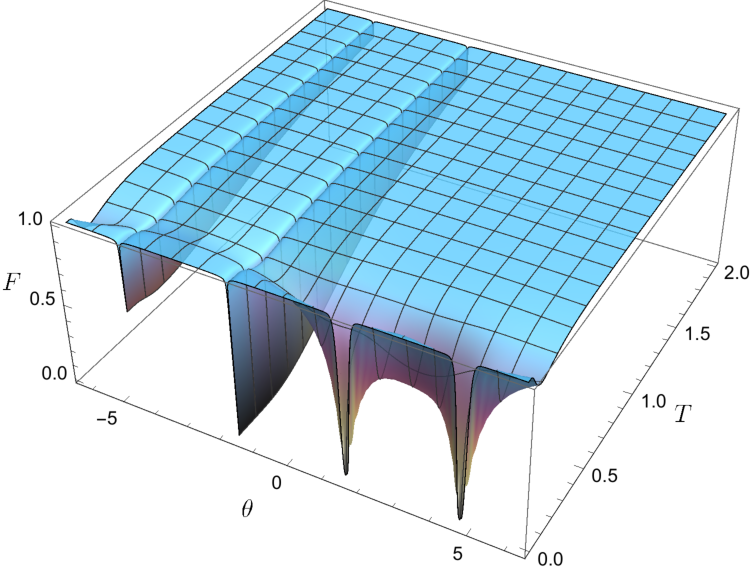
\includegraphics[width=0.20\textwidth,height=0.15\textwidth]{plot3}
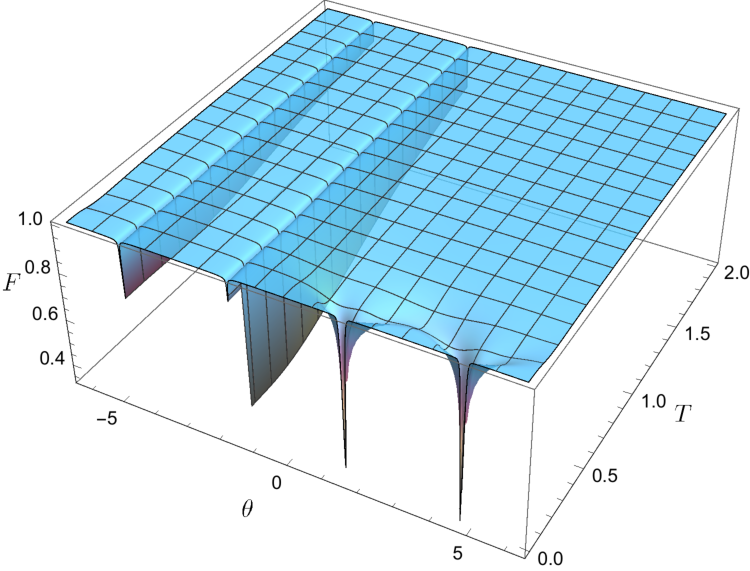
\includegraphics[width=0.20\textwidth,height=0.15\textwidth]{plot4}
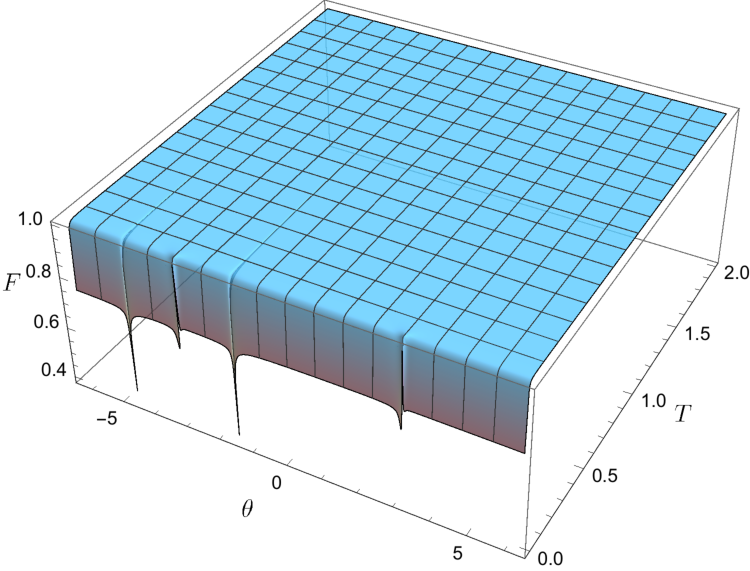
\includegraphics[width=0.20\textwidth,height=0.15\textwidth]{plot1}
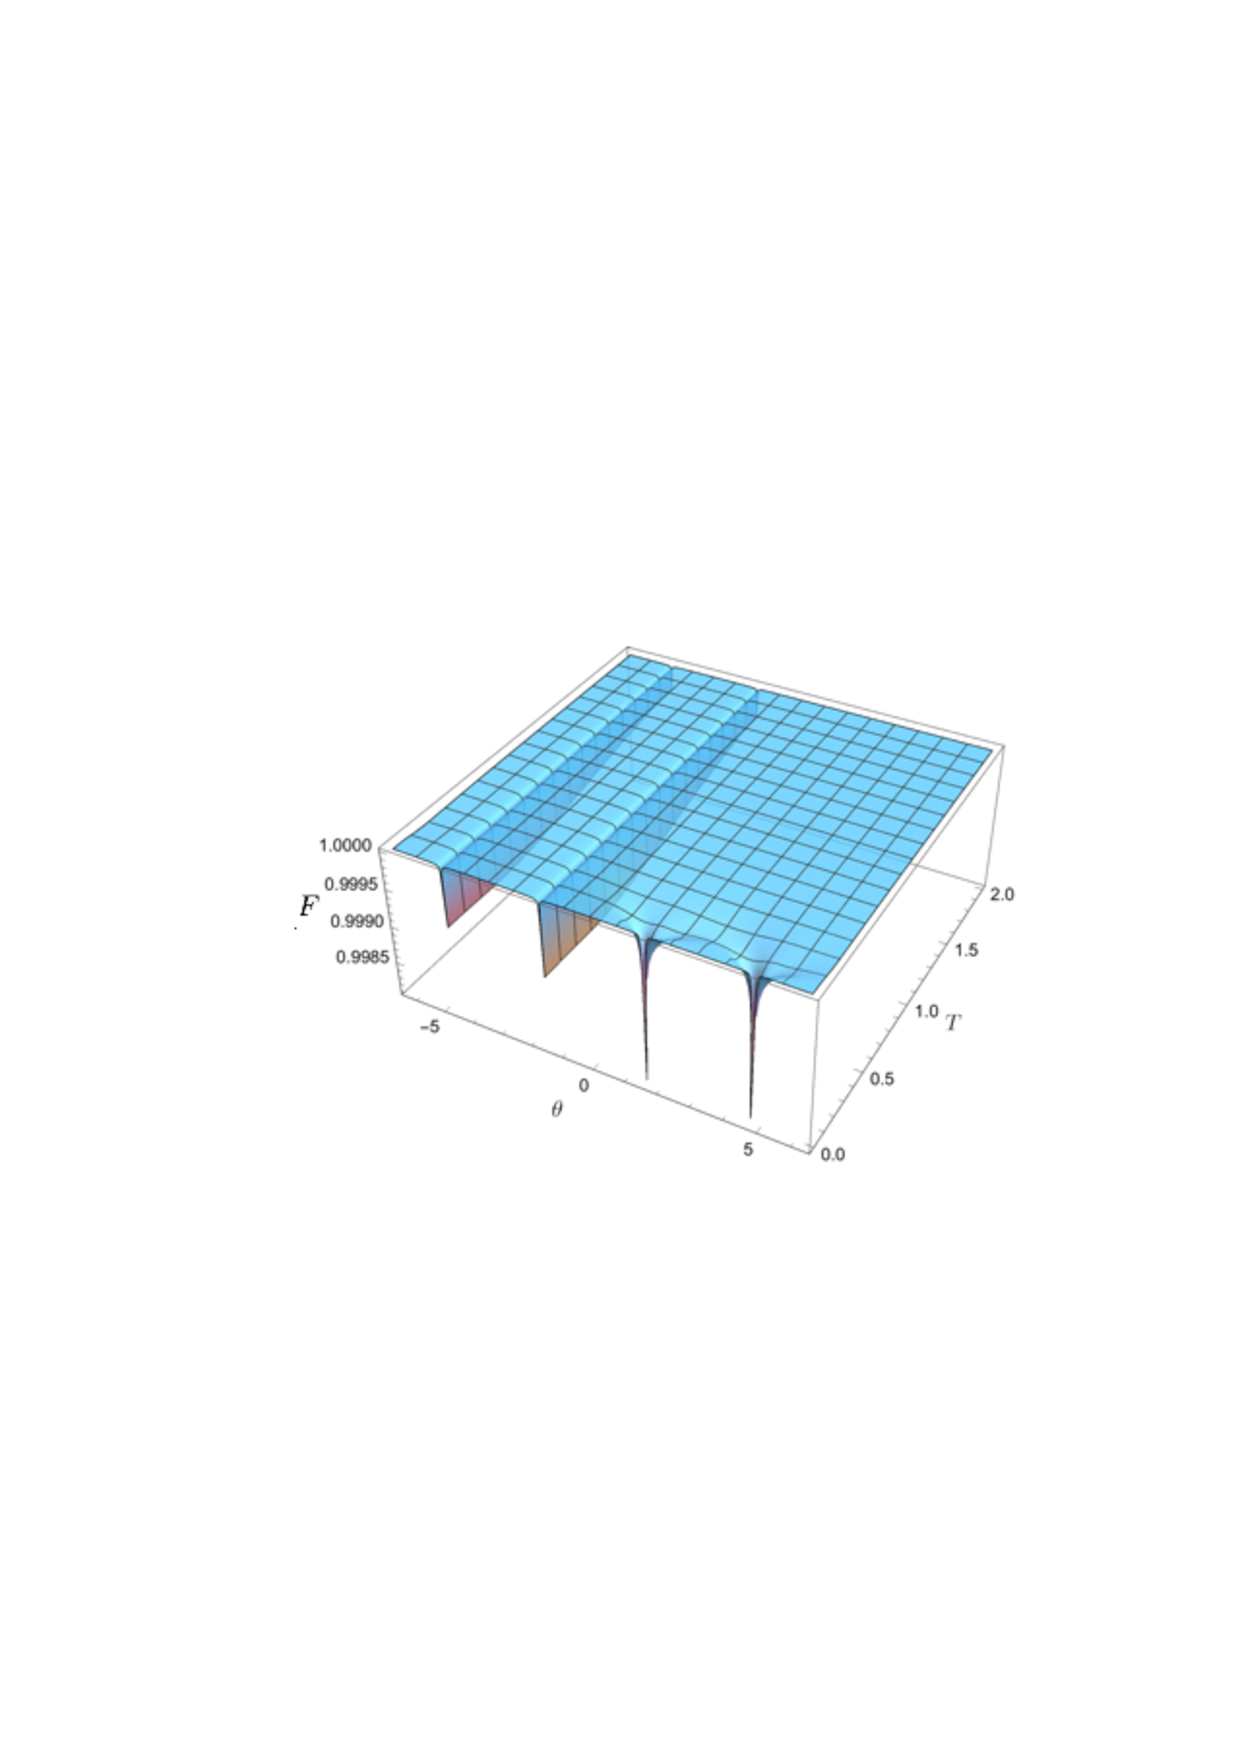
\includegraphics[width=0.20\textwidth,height=0.15\textwidth]{plot2}
\end{flushleft}
\end{minipage}
\begin{minipage}{1.22\textwidth}
\begin{flushleft}
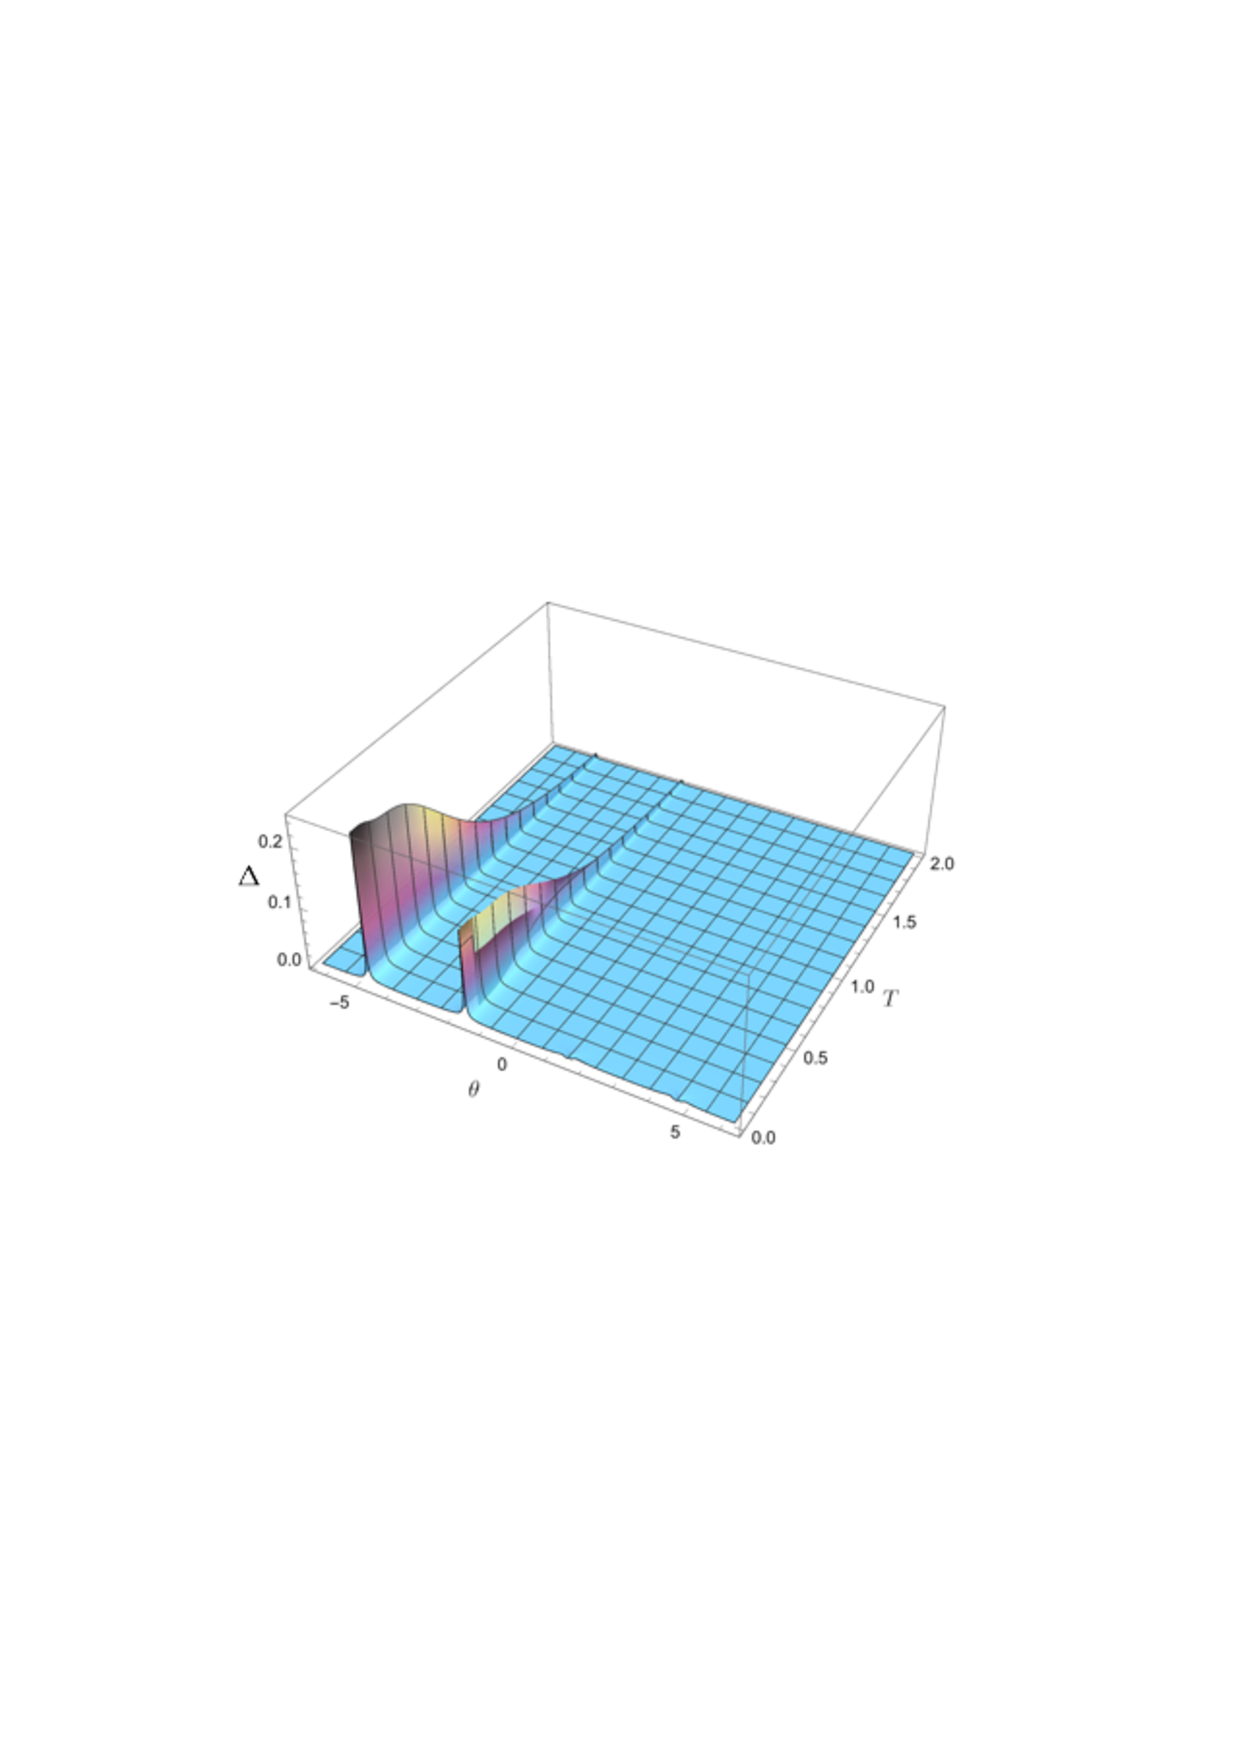
\includegraphics[width=0.20\textwidth,height=0.15\textwidth]{plot7}
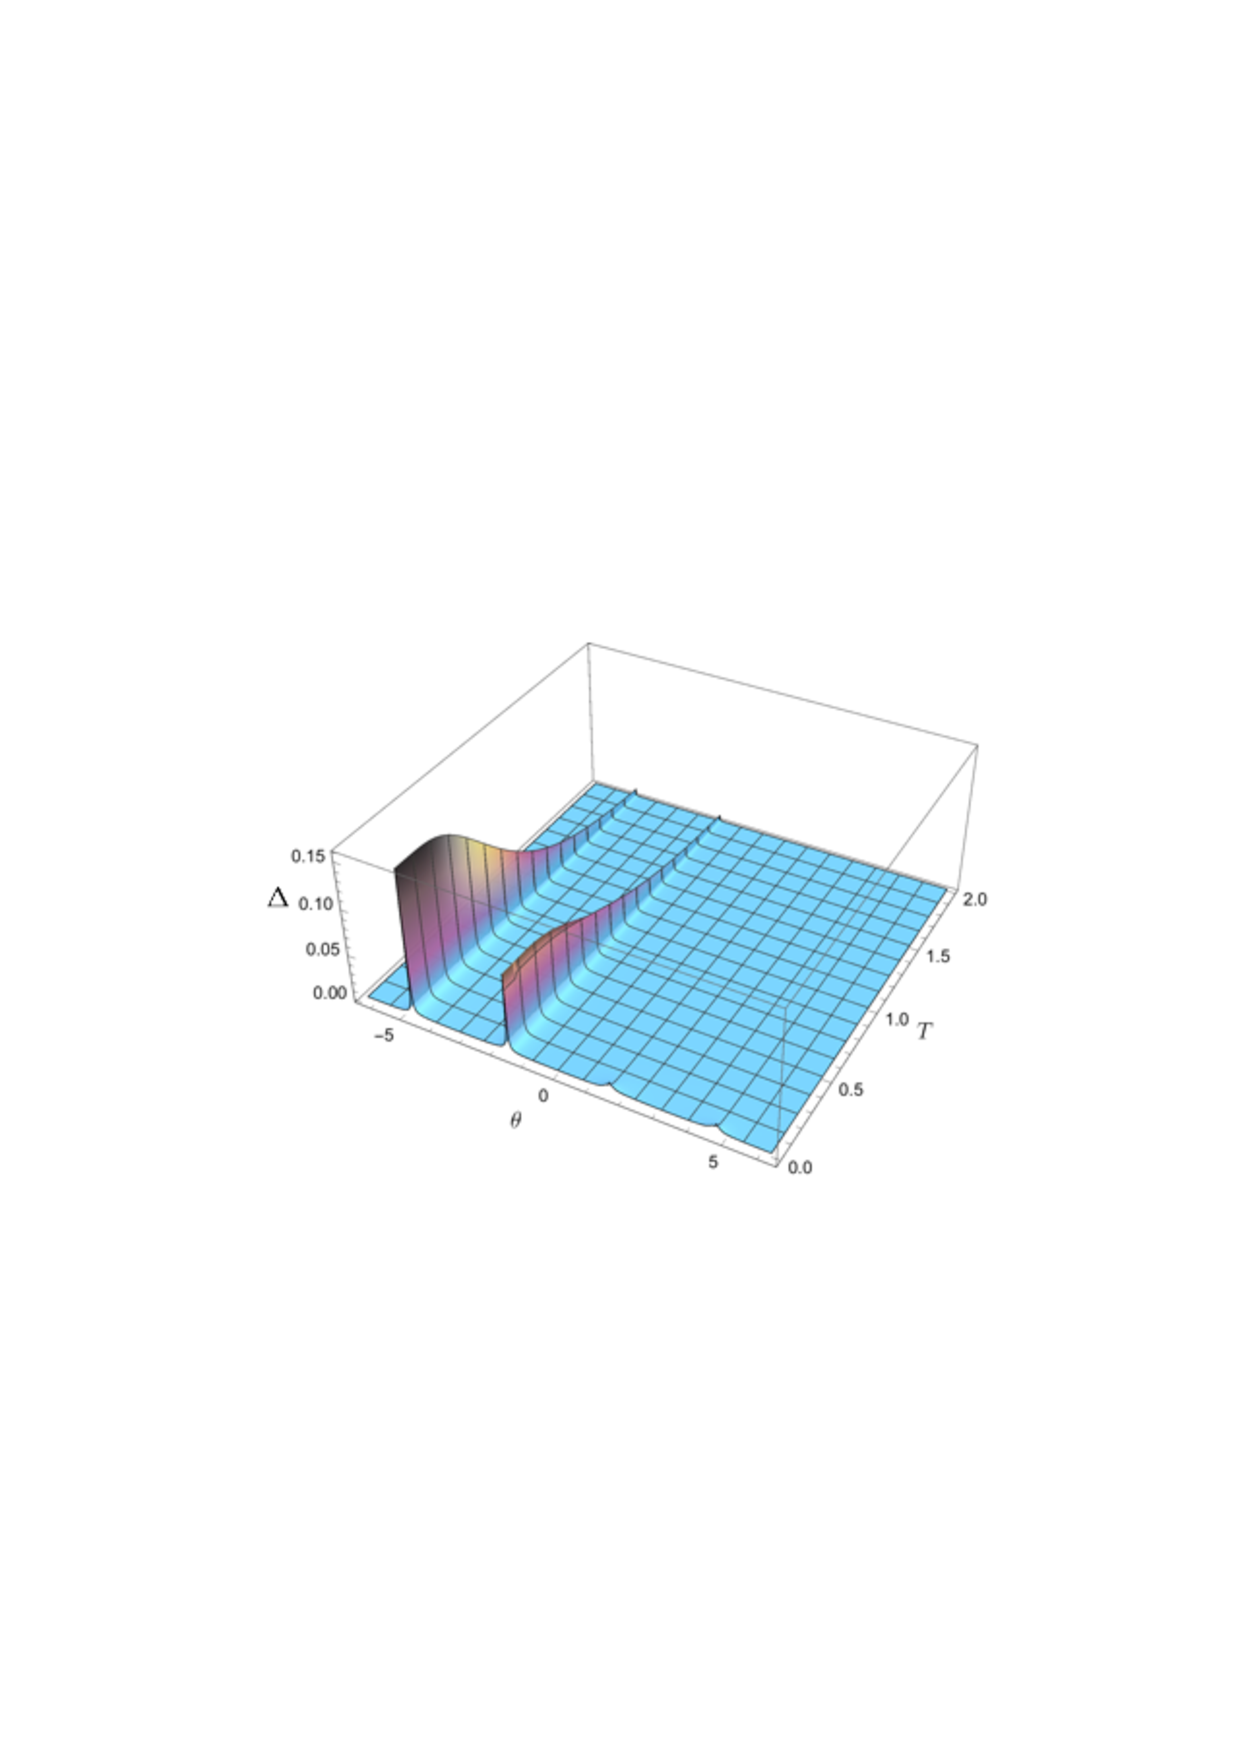
\includegraphics[width=0.20\textwidth,height=0.15\textwidth]{plot8}
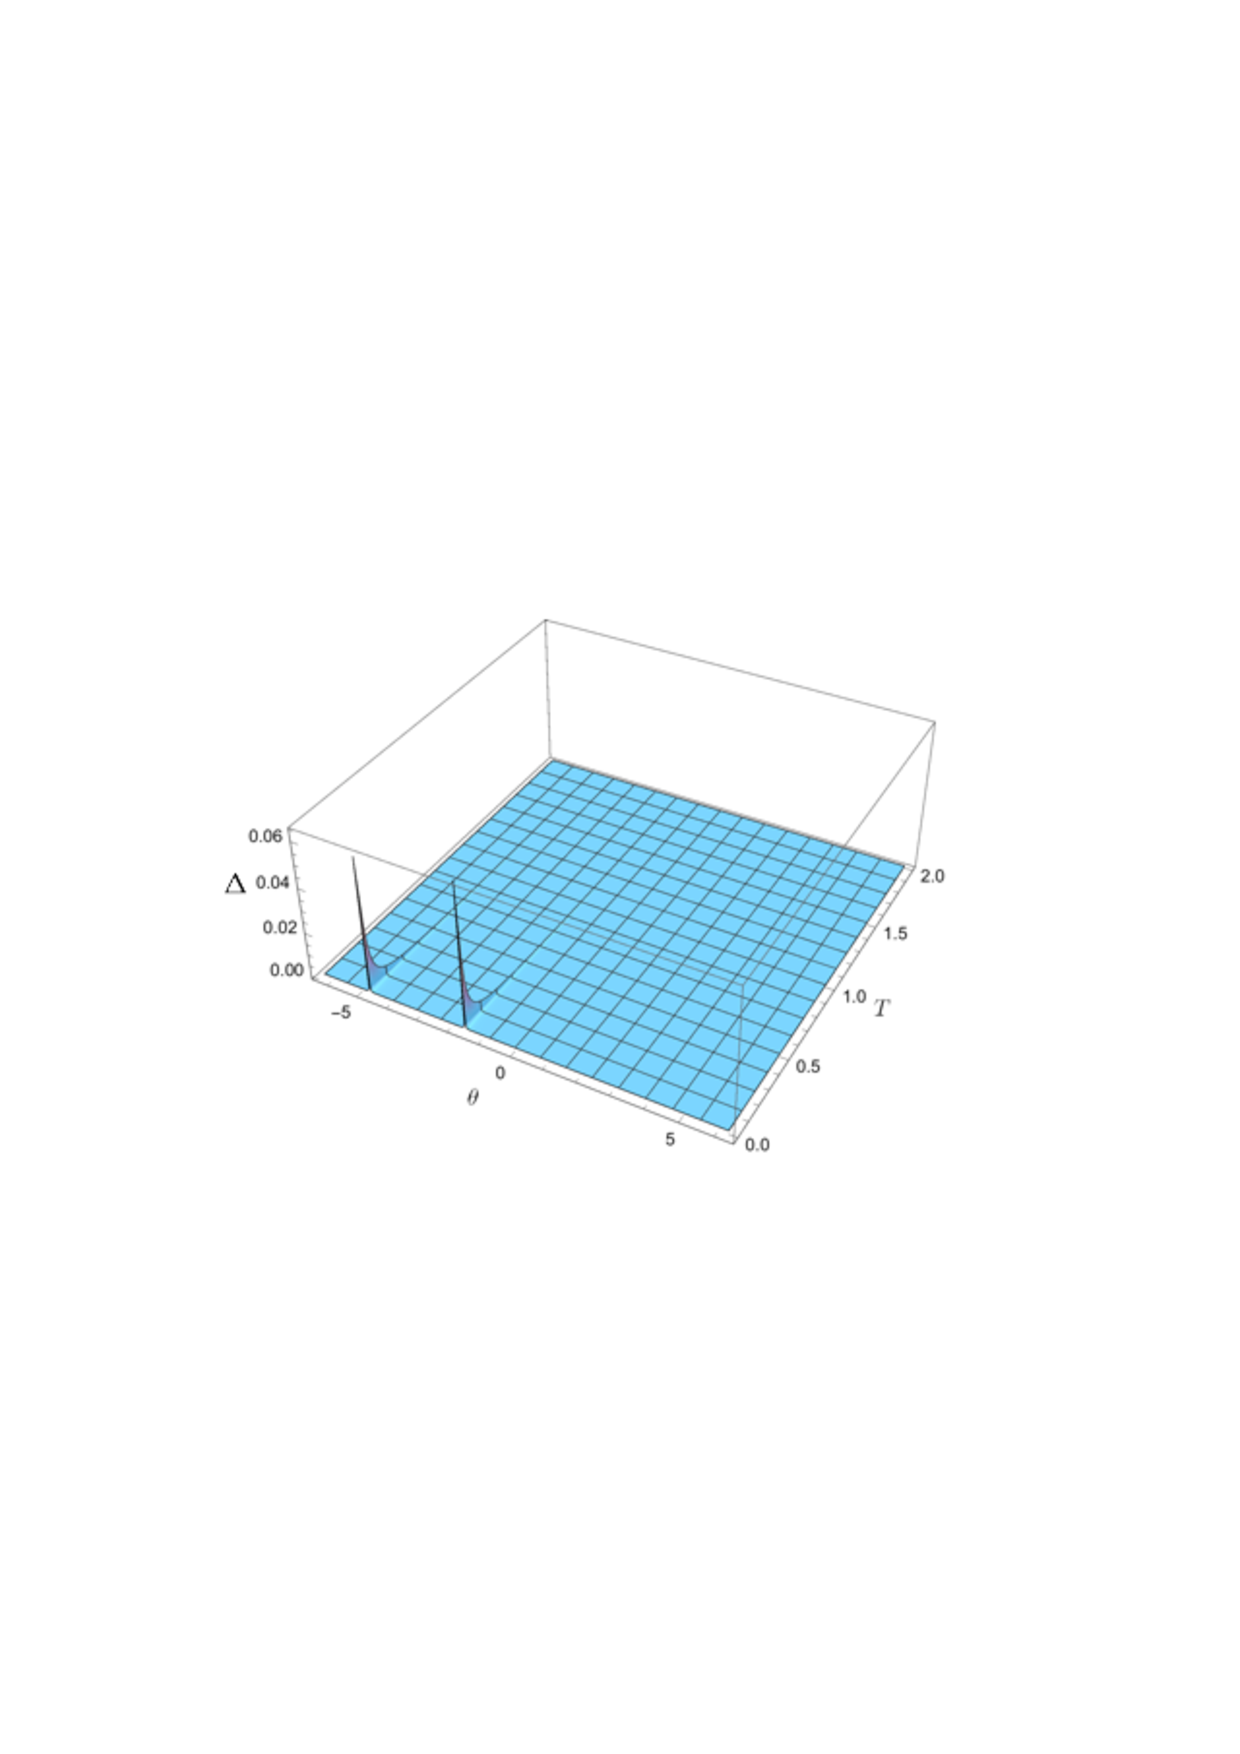
\includegraphics[width=0.20\textwidth,height=0.15\textwidth]{plot5}
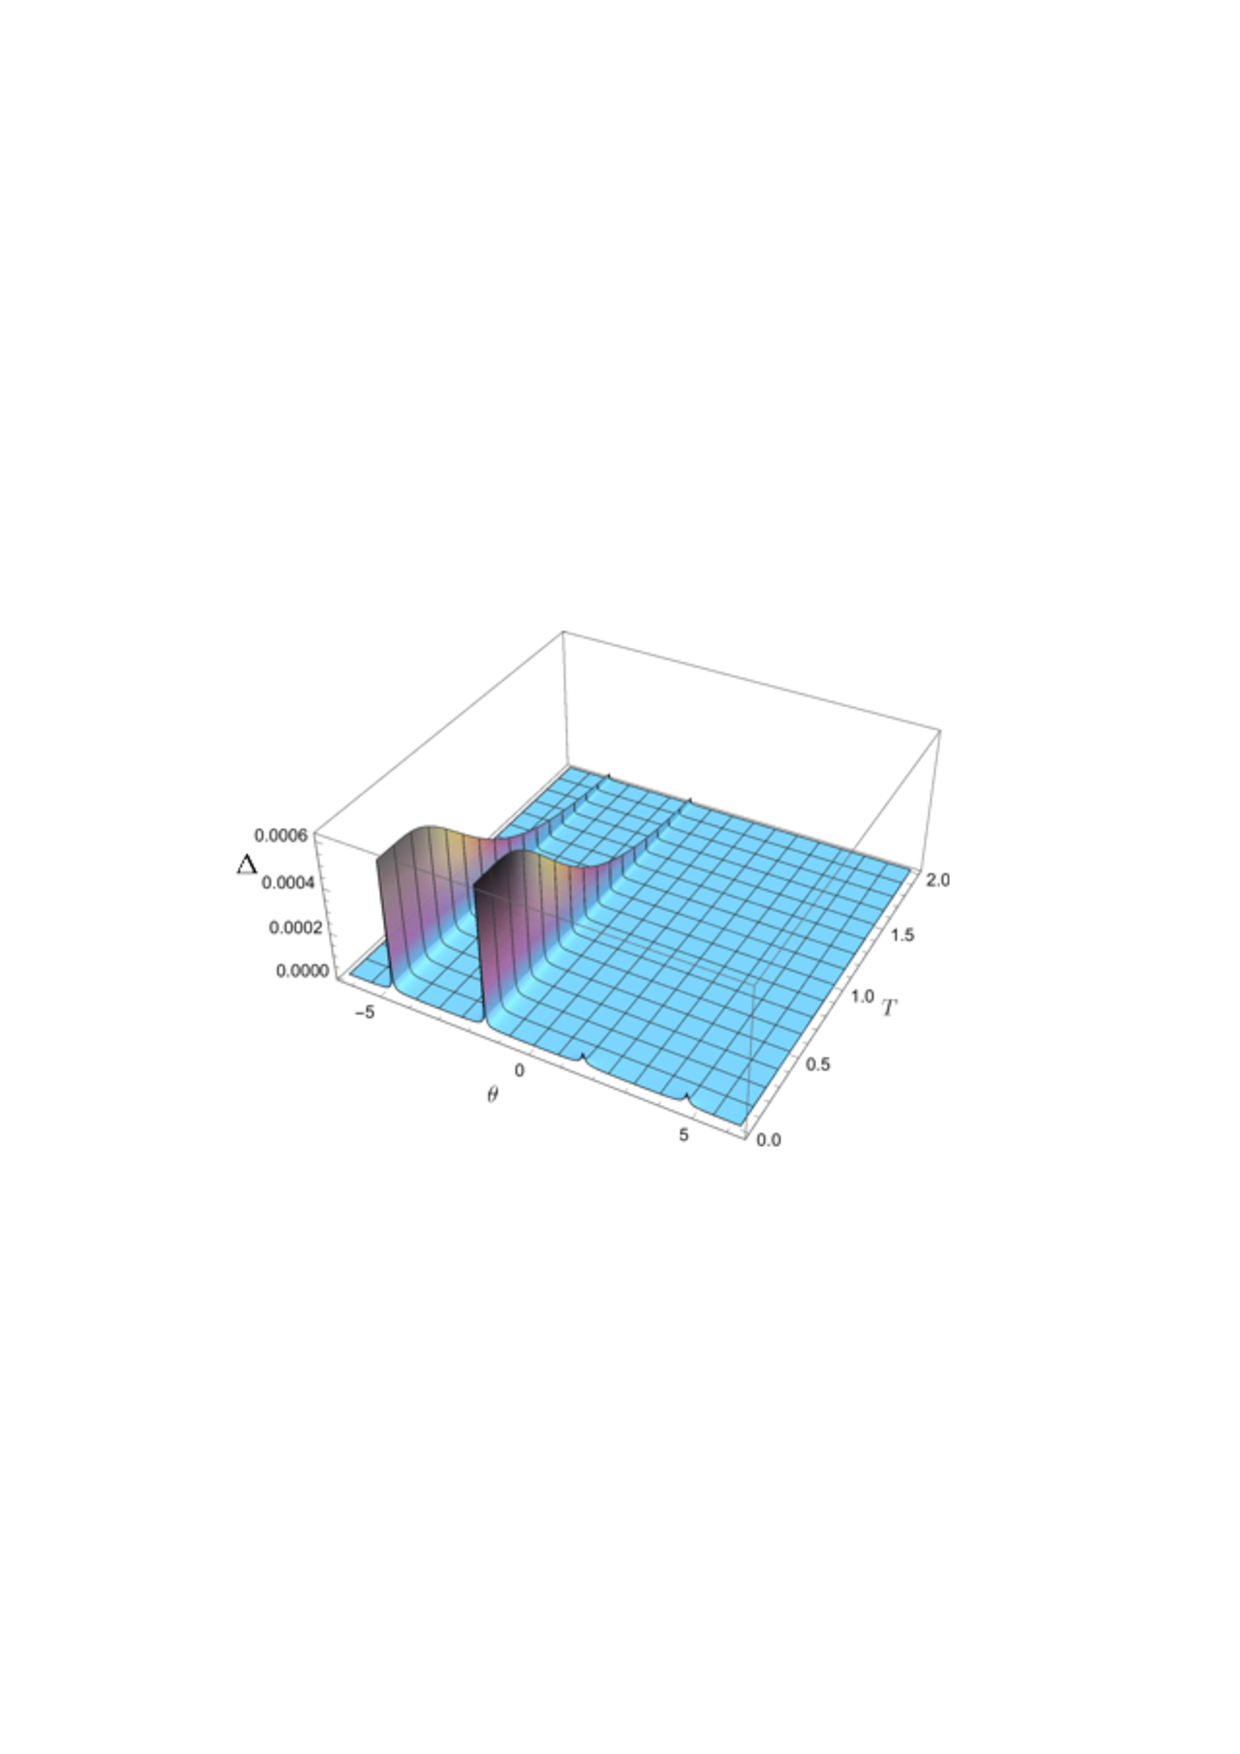
\includegraphics[width=0.20\textwidth,height=0.15\textwidth]{plot6}
\end{flushleft}
\end{minipage}
\begin{minipage}{1\textwidth}	
\caption{Fidelity (top) and $\Delta$ (bottom) for the many-body states $\varrho^{(0)}$ (left) and $\varrho^{(1)}$ (middle-left) and the single-particle states $\rho^{(0)}$ (middle-right) and $\rho^{(1)}$ (right), for the BDI symmetry class. $\delta \theta =\theta'-\theta=0.01$ and $\delta T=T'-T=0.01$. The small step in the top middle-left plot is due to numerical instability.}
\label{fig:fidelityBDI}
\end{minipage}
\end{figure}

\begin{figure}[h!]
\center
\begin{minipage}{1.22\textwidth}
\begin{flushleft}
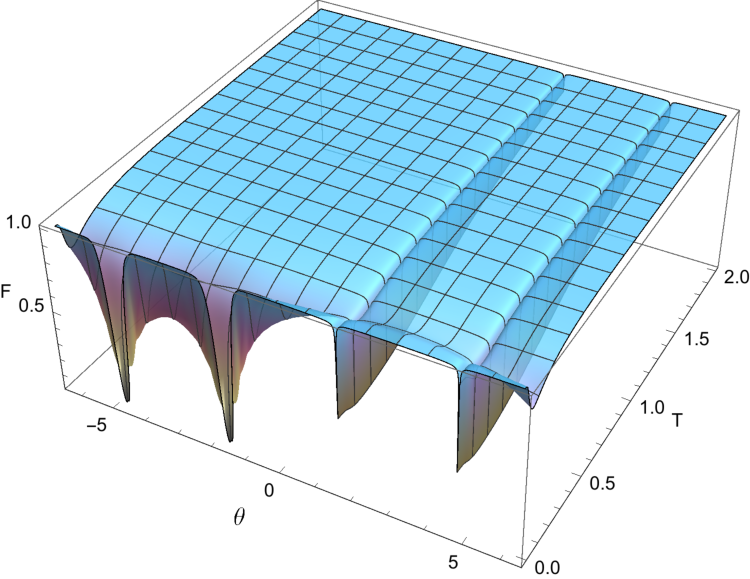
\includegraphics[width=0.20\textwidth,height=0.15\textwidth]{a3fidm0}
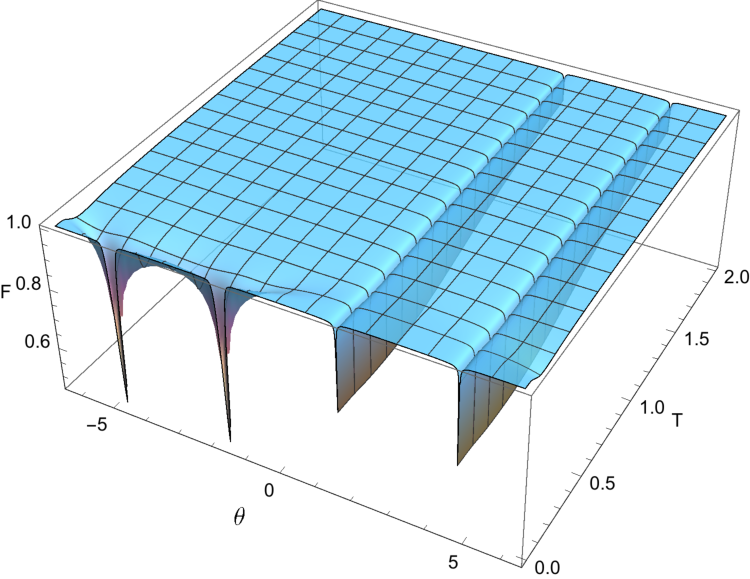
\includegraphics[width=0.20\textwidth,height=0.15\textwidth]{a3fidm1}
\includegraphics[width=0.20\textwidth,height=0.15\textwidth]{a3fids0}
\includegraphics[width=0.20\textwidth,height=0.15\textwidth]{a3fids1}
\end{flushleft}
\end{minipage}
\begin{minipage}{1.22\textwidth}
\begin{flushleft}
\includegraphics[width=0.20\textwidth,height=0.15\textwidth]{a3uhlm0}
\includegraphics[width=0.20\textwidth,height=0.15\textwidth]{a3uhlm1}
\includegraphics[width=0.20\textwidth,height=0.15\textwidth]{a3uhls0}
\includegraphics[width=0.20\textwidth,height=0.15\textwidth]{a3uhls1}
\end{flushleft}
\end{minipage}
\begin{minipage}{1\textwidth}	
\caption{Fidelity (top) and $\Delta$ (bottom) for the many-body states $\varrho^{(0)}$ (left)  and $\varrho^{(1)}$ (middle-left), and the single-particle states $\rho^{(0)}$ (middle-right) and $\rho^{(1)}$ (right), for the AIII symmetry class. $\delta \theta =\theta'-\theta=0.01$ and $\delta T=T'-T=0.01$. In the case of the state $\rho^{(1)}$, the quantity $\Delta$ is highly oscillating for temperatures close to $0$ in the neighbourhood of the critical points, therefore we show the results for a range of temperatures where these numerical instabilities are less prominent.}
\label{fig:fidelityAIII}
\end{minipage}
\end{figure}


A unique feature of periodically driven systems and their corresponding effective Hamiltonians is that both energies $E_k = 0$ and $E_k = \pi$ correspond to a closed gap (the difference between the two energy levels $\pm E_k$ becomes zero modulo $2\pi$). This special feature of QWs yields a surprising result in our analysis. In our study, we observe a different behaviour of the gap closing points with temperature, depending on whether they correspond to $E_k = 0$ (the two points with $\theta > 0$) or $E_k = \pi$ energy (the two points with $\theta < 0$). 
 Whenever the gap closes, the vector $\vec{n}_k(\theta)$ is ill-defined, but the behaviour of $F$ and $\Delta$ will be different due to their dependence on the entire energy spectrum. For the case of $E_k = 0$, they signal two isolated zero-temperature points of quantum PTs, corresponding to $\theta = \pi /2,\ 3\pi /2$ (in the case of $\Delta$ we notice small, but still present, peaks at these points). As the temperature increases, they are no longer signalling a PT and this is due to the dependence on the hyperbolic sine of $E_k$, which vanishes for $E_k=0$ (see the respective formulae), thus eliminating the $\vec {n}_k\cdot \vec {n}'_k$ term carrying the relevant topological features. The significance of these points of the zero-temperature quantum PTs on the system in the low-temperature regime, and the existence of possible crossovers, remain as open questions and require further investigation. In contrast to that, for the $E_k=\pi$ gap closing points, the PT lines survive with temperature, hence revealing a ``finite-temperature quantum PT'' (a PT occurring at finite temperature, driven solely by the Hamiltonian's parameter(s), and not the temperature). Again, this can be understood through the dependence on $E_k$ via hyperbolic functions which take finite values for $E_k=\pi$, thus maintaining the dependence on $\vec{n}_k\cdot\vec{n}'_k$.
 
 Notice that for $\rho^{(0)}$ the qualitative behaviour is different from the other three types of states: the fidelity does not drop for $T=0$ and $\theta = \pi /2, 3\pi /2$, while it does for two new $T=0$ points at $\theta = \pm\pi$. The first difference is due to the fact that the zero temperature limit of $\rho^{(0)}$ projects only onto $M$ given by the points of minimum energy $-E_k=-\pi$, see Equation~\eqref{eq:rho0_lim}. Thus, both quantities do not see the critical momentum at which the gap closes at zero energy, which is above the lowest mode. The abrupt change of the fidelity at the points where $\theta=\pm \pi$ is the consequence of the enhanced zero-temperature ground state distinguishability due to the fact that $E_k$ becomes constant and independent of $k$, i.e.,  the zero-temperature state projects onto the whole Brillouin zone ($M(\theta = \pm\pi) = \mathcal B$). Notice also that in the respective plot for $\Delta$, the absence of peaks at $\theta = \pm\pi$ is consistent with the fact that the Uhlmann factor quantifies the change of eigenvectors, while the presence of two peaks at the corresponding fidelity plot is due to the flattening of the spectrum, i.e., solely to the change of eigenvalues. Observe that while the results for the representatives of BDI and AIII classes are qualitatively similar, the zero-temperature fidelity corresponding to the $\rho^{(0)}$ states for the AIII representative only exhibits drops in the gap closing points ($-E_k=-\pi$), as the spectrum is always non-trivially $k$-dependent.
 
Let us now comment on the results for the fidelity and the quantity $\Delta$, in the case where we probe the system with respect to the parameter of the Hamiltonian and the temperature, separately. In the first case, where $\delta\theta=0.01$ and $\delta T=0$ ($\delta\vec{q}=(0.01,0)$), the results are qualitatively the same as the ones presented in Figures~\ref{fig:fidelityBDI} and~\ref{fig:fidelityAIII} for $\delta\vec{q}=(0.01,0.01).$ In the second case, where we probe the system only with respect to temperature, that is $\delta\theta=0, \delta T=0.01$ or more concisely $\delta\vec{q}=(0,0.01),$ the results for the fidelity are qualitatively the same as the ones for $\delta\vec{q}=(0.01,0.01),$ while the results for the quantity $\Delta$ are different. In particular, we obtain that $\Delta$ is equal to zero everywhere. This triviality is due to the fact that $\Delta$ quantifies the difference between the eigenbases of $\rho$ and $\rho'$, as mentioned before and in this case that we only change the temperature and not the parameter of the Hamiltonian, the eigenbasis remains the same. On the other hand, the fidelity drops at the points of the PT, since it is also sensitive to changes in the spectrum. Notice that the results for these two cases are in agreement with the results presented in the previous Chapter 4, which were also obtained by separately probing the system with respect to the temperature and the Hamiltonian parameter.
\section{The edge states} 
\label{sec:edgeqw}
We proceed to our study of the edge states. The bulk-to-boundary correspondence principle~\cite{x:g:wen:91,ryu:hat:02} predicts their existence on the boundary between distinct topological phases. These states are symmetry protected, i.e., they are robust against perturbations of the Hamiltonian which respect the symmetries of the system. In the case of pure states, QWs realise the aforementioned principle as shown in~\cite{kit:rud:ber:dem:10,kit:12}. In particular, the authors made $\theta$ change along the line, as 
$\theta(x) = \theta^{(t)}H(x_0-x) + \theta^{(n)}H(x-x_0)$, where $H(x-x_0)$ is the Heaviside step function and $\theta^{(t/n)}$ are the values of the angle for the trivial/non-trivial phase, respectively. This way, they were able to create a phase boundary at the site $x_0$ of the line, where $\theta$ changes. The edge states are then observed by evolving the walk \textit{in time} from the initial state localised at the phase boundary: the probability to find the system in the initial position keeps being (considerably) higher than for the rest of the line, due to the overlap between the initial state with the edge state that is localised there.

In our case, we are interested in probing the robustness of the edge states with respect to temperature. Therefore, we study an ensemble of the BG type which corresponds to a stationary state of the split-step QWs realising the BDI and AIII class representatives, with the position-dependent coin operation, parameterised by its temperature $\beta^{-1}$. This stationary state appears naturally if one looks at the von Neumann evolution equation for the density matrix and imposes the stationarity condition. By diagonalising $H_{\text{eff}}$ we obtain the localised states which can either have quasienergy $0 \text{ or }\pi$. Here, we choose a different order for the energy spectrum, by promoting the edge states with energies $E=\pi$ and $E = 0$ to be ground states, so that they survive at the zero-temperature limit. 

\begin{figure}[h!]
\center
\includegraphics[scale=0.4]{edgestates_BDI}
\caption{
Position probability distribution of the QW simulating the representative of the BDI class, as a function of the sites, $\tr (e^{-H/T}\ket{x}\bra{x})/Z$. The Hamiltonian $H$ is obtained by varying $\theta$ along $x$ through a step-like function~\cite{kit:rud:ber:dem:10}. The domain wall is centred in the middle of the line. Periodic boundary conditions are taken, hence the edge state at the boundary.}
\label{fig:edgeBDI}
\end{figure}

\begin{figure}[h!]
\center
\includegraphics[width=0.6\textwidth,height=0.25\textwidth]{plot9.pdf}
\caption{Position probability distribution of the QW simulating the representative of the AIII class, as a function of the sites, $\tr (e^{-H/T}\ket{x}\bra{x})/Z$. Again, the parameter $\theta$ of the Hamiltonian, changes along $x$ according to a step-like function~\cite{kit:rud:ber:dem:10}. The boundary  is centred in the middle of the line and periodic boundary conditions are taken.}
\label{fig:edgeAIII}
\end{figure}


We observe that at $T=0$, the edge state has the major contribution to the probability distribution. As temperature increases, the edge states are smeared out, see Figure~\ref{fig:edgeBDI} for the BDI class representative and Figure~\ref{fig:edgeAIII} for the representative of the class AIII. Since the presence of an edge state is a clear manifestation of the topological order at $T=0$, the fact that it does not disappear for higher temperatures, but it is rather smeared out, suggests that the topological nature of the system is preserved in agreement with the fidelity and $\Delta$ analysis for the $E_k=\pi$ gap-closing points.

Our fidelity and $\Delta$ analysis revealed that for $T>0$ there exist no thermal PTs (i.e., no temperature-driven PTs), as also shown in Chapter 4 for paradigmatic models of TIs and TSCs. However, here we observe finite temperature \emph{parameter}-driven PTs. The non-existence of thermal PTs is further confirmed by the behaviour of the edge states, which are gradually smeared out as temperature increases, as also pointed out in~\cite{viy:riv:del:14}. Note that the edge states studied here are probed through a different method from the one used in Chapter 4. There, a small chemical potential was introduced in such a way that the zero-temperature behaviour of the many-body density operator is the projector onto the Fermi sea. Consequently, the existence of the edge states was signalled by the abrupt change in the number operator on the sites where they appeared.





\section{Conclusions}
\label{Conclusions and Outlook}
We derived analytic expressions for the fidelity and the quantity $\Delta$ between two BG states for QW representatives of topological phases for the chiral symmetric classes BDI and AIII and their many-body counterparts. For the systems considered, the fidelity is detecting the points where the Bloch vector is ill-defined, which corresponds to the closure of the gap. Since in our case the phase diagram is such that the closure of the gap always means the change from a trivial phase to a nontrivial one, and vice versa, the fidelity is capturing the topological PT. Our results show the absence of temperature-driven PTs in two ways: through the fidelity analysis and through the behaviour of the edge states appearing on the phase boundary. In addition, the analysis of the fidelity and, through the quantity $\Delta$, the Uhlmann connection shows the existence of finite-temperature PTs driven solely by the Hamiltonian's parameter $\theta$. We would also like to point out that, providing that one of the goals of this study is to investigate the finite-temperature behaviour of topological order in realistic many-body systems, the fact that the behaviour of the single-particle BG states is consistent with that of their many-body counterparts, shows that the analysis of the former can be a useful mathematical tool in the study of the latter.

Finally, we would like to point out some possible future lines of research. First, the same study could be applied to the rest of the symmetry classes in 1D and 2D using the protocols introduced in~\cite{kit:rud:ber:dem:10}. Further analysis of realistic noise effects that can give rise to these BG states, in particular the single-particle ones, presents another interesting line of research (for a partial answer to this question, see also a recent study of the effects of thermal noise onto single-particle factor states of a topological insulator~\cite{riv:viy:del:13}). The above study could also be conducted for 2D QWs, as well as in the realm of multi-particle QWs.\\



%
%
%\bibliography{bibforthesis}
%\bibliographystyle{unsrt}
%
%\end{document}

%%\documentclass[11pt]{report}
%\linespread{1.3} %1.3 for one and a half spacing, 1.6 for double
%\usepackage{amsmath, amsthm, amssymb, float, graphicx, caption, subcaption, cite, braket, url,color}
%%\usepackage[nohug,heads=vee]{diagrams}
%%\diagramstyle[labelstyle=\scriptstyle]
%%\graphicspath{{./Figures/}}
%\usepackage[margin=2.5cm]{geometry}
%%\title{Title}
%%\author{Chrysoula Vlachou}
%%\date{}
%\newtheorem{lemma}{Lemma}
%\newtheorem{theorem}{Theorem}
%\newtheorem{proposition}{Proposition}
%
%\newtheorem{definition}{Definition}
%\newcommand{\N}{\mathbb N}
%\newcommand{\R}{\mathbb R}
%\newcommand{\C}{\mathbb C}
%\newcommand{\Hilb}{\mathcal H}
%\newcommand{\HRule}{\rule{\linewidth}{0.5mm}}
%\newcommand{\mmobh}{\textlatin{M\"ob}(\mathbb{H})}
%\newcommand{\areah}{\textlatin{area}_{\mathbb{H}}}
%\newcommand{\dth}{d_{\mathbb{H}}}
%\newcommand{\tdth}{$d_{\mathbb{H}}$ }
%\def\h{\mathbb H}
%\DeclareMathOperator{\tr}{Tr}
%\def\I{\hat I}
%\def\ds{\displaystyle}
%\def\ppmod{\!\!\!\!\!\pmod}
%\newcommand{\q}[1]{\vec{#1}\cdot\vec{\sigma}}
%\usepackage{mathrsfs}
%
%
%\newcommand{\innerproduct}[2]{\langle #1 | #2 \rangle}
%\def\mobh{\textlatin{M\"ob}({\mathbb H})}
%
%
%
%\begin{document}
\chapter{Phase transitions at finite temperatures of topological systems out of equilibrium}

 



In this chapter, we investigate the existence of finite-temperature PTs in topological systems out of equilibrium. As mentioned in the Introduction, recently, there have been proposed two different approaches to DPTs, which give opposite predictions. Our goal is to compare and contrast these two approaches and clarify which is the one that better captures the many-body nature of these systems.
This chapter is organised as follows: in Section~\ref{Sec: DQPTs and Susceptibilities}, after a brief introduction to the study of DQPTs in the case of pure states, we proceed by analytically deriving the two different finite-temperature generalisations of the LE (fidelity LE and interferometric LE) and the associated susceptibilities, which give opposite predictions about the fate of DQPTs in the case of mixed states. Subsequently, we specialise this derivation in the case of two-band Hamiltonians, since the topological systems that we are interested in are described by such Hamiltonians. Based on the analysis of the two different dynamical susceptibilities, we compare the two approaches to DPTs, analyse the reasons for their different predictions and argue that the fidelity LE approach is more suitable in the case of realistic many-body systems.  
In Section~\ref{sec:num.results}, we present quantitative results for the fidelity-induced first time derivative of the rate function in the case of the 1D SSH model~\cite{su:sch:hee:79} of a TI and the 2D Massive Dirac (MD) model of a Chern insulator~\cite{qi:hug:zha:08}. Finally, in the last section we summarise our results and present our conclusions.\\  
\vfill

\begin{center}
 *The work presented in this chapter corresponds to the work published in~\cite{mer:vla:pau:vie:viy:18}.
\end{center}

\newpage


\section{Dynamical (quantum) phase transitions and the associated susceptibilities}
\label{Sec: DQPTs and Susceptibilities}
The authors in~\cite{hey:pol:keh:13} introduce the concept of DQPTs and illustrate their properties in the case of the transverse-field Ising model. They observe a similarity between the partition function of a quantum system in equilibrium, $Z(\beta)=\tr(e^{-\beta H})$, and the overlap amplitude of some time-evolved initial quantum state $\ket{\psi_i}$ with itself, $G(t)=\langle\psi_i|e^{-iHt}|\psi_i\rangle$. During a temperature-driven PT, the abrupt change of the properties of the system is indicated by the non-analyticity of the free energy density $f(\beta)=-\lim_{N\to\infty}\frac{1}{N}\ln Z(\beta)$ at the critical temperature ($N$ being the number of degrees of freedom). It is then possible to establish an analogy with the case of the real-time evolution of a quantum system out of equilibrium, by considering the rate function 
\begin{equation}
\label{eq:rate}
g(t)=-\frac{1}{N}\log |G(t)|^2,
\end{equation} 
where $|G(t)|^2$ is a mixed-state LE, as we detail below. The rate function $g(t)$ may exhibit non-analyticities at some critical times $t_c$, after a quantum quench. 


\subsection{DQPTs for pure states}
\label{Subsec: DQPT for pure states}

At zero temperature, the LE $G(t)$ from Equation~\eqref{eq:rate} between the ground state for $\lambda=\lambda_i\in M$ and the evolved state with respect to the Hamiltonian for $\lambda=\lambda_f\in M$ is given by the fidelity between the two states
\begin{eqnarray}
\mathcal{F}(t;\lambda_{f},\lambda_i)\equiv |\bra{\psi(\lambda_i)}e^{-it H(\lambda_f)}\ket{\psi(\lambda_i)}|.
\label{Eq: zero temperature fidelity}
\end{eqnarray}
For $\lambda_i=\lambda_f$, the fidelity is trivial, since the system remains in the same state. Fixing $\lambda_i\equiv \lambda$ and $\lambda_{f} = \lambda + \delta\lambda$, with $\delta\lambda<<1$, in the $t\rightarrow\infty$ limit Equation~\eqref{Eq: zero temperature fidelity} is nothing but the familiar $S$-matrix with an unperturbed Hamiltonian $H(\lambda)$ and an interaction Hamiltonian $V(\lambda)$, which is approximated by
\begin{eqnarray}
V(\lambda)\equiv H(\lambda_f)-H(\lambda)\approx\frac{\partial H}{\partial \lambda^{a}}(\lambda)\delta \lambda^a.
\label{Eq:2}
\end{eqnarray}
After applying standard perturbation theory techniques (see Appendix B),
 we obtain
\begin{eqnarray}
\mathcal{F}(t;\lambda_f,\lambda)\approx 1 -\chi_{ab}(t;\lambda)\delta \lambda^a \delta \lambda^b,
\end{eqnarray}
where the dynamical susceptibility $\chi_{ab}(t;\lambda)$ is given by
\begin{small}
\begin{eqnarray}
&\chi_{ab}(t;\lambda)=\nonumber \\
&\int_{0}^{t}\int_{0}^{t} dt_2dt_1 \left(\frac{1}{2}\langle \{V_{a}(t_2),V_{b}(t_1)\} \rangle-\langle V_{a}(t_2)\rangle \langle V_{b}(t_1) \rangle\right),
\label{Eq: zero temperature susceptibility}
\end{eqnarray}
\end{small}with $V_{a}(t,\lambda)=e^{it H(\lambda)}\partial H/\partial \lambda^{a}(\lambda)e^{-it H(\lambda)}$ and $\langle \ast\rangle=\bra{\psi(\lambda)}\ast\ket{\psi(\lambda)}$. The family of symmetric tensors $\{ds^2(t)=\chi_{ab}(t,\lambda)d\lambda^a d\lambda^b\}_{t\in \mathbb{R}}$ defines a family of metrics in the manifold $M$, which can be seen as pullback metrics of the Bures metric (Fubini-Study metric) in the manifold of pure states~\cite{chr:jam:12}. Specifically, at time $t$, the pullback is given by the map $\Phi_t: \lambda_f \mapsto e^{-it H(\lambda_f)}\ket{\psi(\lambda)}\bra{\psi(\lambda)}e^{i t H(\lambda_f)}$, evaluated at $\lambda_f=\lambda$.
 
\subsection{Generalisations at finite temperatures}
\label{Subsec: DQPT for pure states}


The generalisation of DQPTs to mixed states is not unique. There are several ways to construct a LE for a general density matrix. In what follows, we derive two finite-temperature generalisations, such that they have the same zero-temperature limit. \\
\subsubsection{Fidelity Loschmidt Echo at $T>0$}


First, we introduce the {\em fidelity LE} between the state $\rho(\beta;\lambda_i)=e^{-\beta H(\lambda_i)}/\tr\{e^{-\beta H(\lambda_i)}\}$ and the one evolved by the unitary operator $e^{-it H(\lambda_f)}$ as
\begin{eqnarray}
\!\!\!\!\!\!\mathcal{F}(t,\beta;\lambda_i,\lambda_f)\!=\!F(\rho(\beta;\lambda_i),e^{-it H(\lambda_f)}\rho(\beta;\lambda_i)e^{itH(\lambda_f)}),
\label{eq:fid}
\end{eqnarray}
where $F(\rho,\sigma)=\tr\{\sqrt{\sqrt{\rho}\sigma\sqrt{\rho}}\}$ is the quantum fidelity between arbitrary mixed states $\rho$ and $\sigma$. For $\lambda_f$ close to $\lambda_i=\lambda$, we can write
\begin{eqnarray}
\mathcal{F}(t,\beta ;\lambda_f,\lambda)\approx 1 -\chi_{ab}(t,\beta ;\lambda)\delta \lambda^a \delta \lambda^b,
\end{eqnarray}
with $\chi_{ab}(t,\beta,\lambda)$ being the \emph{Dynamical Fidelity Susceptibility} (DFS). Notice that $$\lim_{\beta\to\infty}\chi_{ab}(t,\beta;\lambda)=\chi_{ab}(t;\lambda),$$ where $\chi_{ab}(t;\lambda)$ is given by Equation~\eqref{Eq: zero temperature susceptibility}. At time $t$ and inverse temperature $\beta$, we have a map $\Phi_{(t,\beta)}: \lambda_f\mapsto e^{-i tH (\lambda_f)} \rho(\beta;\lambda) e^{it H(\lambda_f)}$. The $2$-parameter family of metrics defined by $ds^2(\beta,t)=\chi_{ab}(t,\beta;\lambda)d\lambda^{a}d\lambda^b$ is the pullback by $\Phi_{(t,\beta)}$ of the Bures metric on the manifold of full-rank density operators, evaluated at $\lambda_f=\lambda$ (see Appendix B).

The fidelity LE is closely related to the Uhlmann connection: $F(\rho_1,\rho_2)$ equals the overlap between purifications $W_1$ and $W_2$, $\langle W_1,W_2\rangle=\tr \left\{W_1^\dagger W_2\right\}$, satisfying discrete parallel transport condition (see, for instance,~\cite{uhl:11}). 


\subsubsection{Interferometric Loschmidt Echo at $T>0$}

Here, we consider an alternative generalisation of the LE for mixed states [$G(t)$ from Equation~\eqref{eq:rate}]. In particular, we define the {\em interferometric LE} as
\begin{eqnarray}
\mathcal{L}(t,\beta ;\lambda_{f},\lambda_i)=\left|\frac{\tr\left\{e^{-\beta H(\lambda_i)} e^{i tH(\lambda_i)}e^{-i t H(\lambda_f)}\right\}}{\tr \left\{e^{-\beta H(\lambda_i)}\right\}}\right|.
\end{eqnarray}
The $e^{it H(\lambda_i)}$ factor does not appear at zero temperature, since it just gives a phase which is canceled by taking the absolute value.  This differs from previous treatments in the literature~\cite{bud:hey:16} (see Section~5.5.4 of~\cite{chr:jam:12}, where the variation of the interferometric phase, $\tr\{\rho_0 e^{-it H}\}$, exposes this structure). However, it is convenient to introduce it in order to have the usual form of the perturbation expansion, as will become clear later.

For $\lambda_f$ close to $\lambda_i=\lambda$, we get
\begin{eqnarray}
\mathcal{L}(t,\beta ;\lambda_f,\lambda)\approx \left|\frac{\tr\left\{e^{-\beta H(\lambda)} T e^{-i \int_{0}^{t} dt' V_{a}(t,\lambda) \delta \lambda^a}\right\}}{\tr \left\{e^{-\beta H(\lambda)}\right\}}\right|,
\end{eqnarray}
so that the perturbation expansion goes as in Equation~\eqref{Eq: zero temperature susceptibility}, yielding
\begin{eqnarray}
\mathcal{L}(t,\beta ;\lambda_f,\lambda)\approx 1 -\tilde\chi_{ab}(t,\beta ;\lambda)\delta \lambda^a \delta \lambda^b,
\end{eqnarray}
with the dynamical susceptibility given by
\begin{small}
\begin{equation}
\tilde{\chi}_{ab}(t,\beta;\lambda)=
\int_{0}^{t}\int_{0}^{t} dt_2dt_1  \left(\frac{1}{2}\langle \{V_{a}(t_2),V_{b}(t_1)\} \rangle-\langle V_{a}(t_2)\rangle \langle V_{b}(t_1) \rangle\right),
\label{Eq: finite temperature interferometric susceptibility}
\end{equation}
\end{small}where $\langle \ast\rangle=\tr\{e^{-\beta H(\lambda)}\ast\}/\tr\{e^{-\beta H(\lambda)}\}$. Notice that Equations~\eqref{Eq: finite temperature interferometric susceptibility} and~\eqref{Eq: zero temperature susceptibility} are formally the same with the average over the ground state replaced by the thermal average. This justifies the extra $e^{it H(\lambda_i)}$ factor. Since this susceptibility comes from the interferometric LE, we call it \emph{Dynamical  Interferometric Susceptibility} (DIS). The quantity $ds^2(\beta,t)=\tilde{\chi}_{ab}(t,\beta;\lambda)d\lambda^ad\lambda^b$ defines a $2$-parameter family of metrics over the manifold $M$, except that they cannot be seen as pullbacks of metrics on the manifold of density operators with full rank. However, it can be interpreted as the pullback by a map from $M$ to the unitary group associated with the Hilbert space of a particular Riemannian metric. For a detailed analysis, see Appendix B. Note that this version of the LE is related to the interferometric geometric phase introduced by Sj\"{o}qvist \emph{ et. al}~\cite{sjo:pat:eke:ana:eri:oi:ved:00,ton:sjo:kwe:oh}. \\

\subsection{Two-band systems}

Many representative examples of TIs and TSCs can be described by effective two-band Hamiltonians. Therefore, we derive closed expressions of the previously introduced dynamical susceptibilities for topological systems within this class. 

The general form of such Hamiltonians is $\{H(\lambda)=\vec{x}(\lambda)\cdot \vec\sigma:\lambda \in M\}$, where $\vec{\sigma} $  is the Pauli vector. The interaction Hamiltonian $V(\lambda)$, introduced in Equation~\eqref{Eq: zero temperature fidelity}, casts the form
\begin{equation*}
V(\lambda)\approx \left(\frac{\partial \vec{x}}{\partial\lambda^a}\cdot \vec{\sigma}\right) \delta \lambda^a.
\end{equation*} 
It is convenient to decompose $\partial\vec{x}/\partial \lambda^a$ into one component perpendicular to $\vec{x}$ and one parallel to it:
\begin{equation*}
\frac{\partial \vec{x}}{\partial\lambda^a}=\left(\frac{\partial \vec{x}}{\partial\lambda^a}\right)^{\perp}+ \left(\frac{\partial \vec{x}}{\partial\lambda^a}\right)^{\parallel}=\vec{t}_{a}+\vec{n}_a.
\end{equation*}
The first term is tangent, in $\mathbb{R}^3$, at $\vec{x}(\lambda)$, to a sphere of constant radius $r=|\vec{x}(\lambda)|$. Hence, this kind of perturbations does not change the spectrum of $H$, only its eigenbasis. The second term is a variation of the length of $\vec{x}$ and hence, it changes the spectrum of $H$, while keeping the eigenbasis fixed. The DFS and the DIS are given by (for the details of the derivation, see Appendix B)
\begin{small}
\begin{eqnarray}
\label{Eq: DFS}
\chi_{ab}&=&\tanh^2(\beta |\vec{x}(\lambda)|)\frac{\sin^2(|\vec{x}(\lambda)|t)}{|\vec{x}(\lambda)|^2}\vec{t}_a\!\!\cdot\!\vec{t}_b \\
\label{Eq: DIS}
\tilde{\chi}_{ab}\!&=&\!\frac{\sin^2(|\vec{x}(\lambda)|t)}{|\vec{x}(\lambda)|^2}\vec{t}_a\!\!\cdot\!\vec{t}_b\!+\!t^2(1\!\!-\!\!\tanh^2(\beta |\vec{x}(\lambda)|))\vec{n}_a\!\!\!\cdot\!\vec{n}_b.
\end{eqnarray}
\end{small}

While the DIS from Equation~\eqref{Eq: DIS} depends on the variation of both the spectrum and the eigenbasis of the Hamiltonian, the DFS from Equation~\eqref{Eq: DFS} depends only on the variations which preserve the spectrum, i.e., changes in the eigenbasis. This is quite remarkable, since in general the fidelity between two quantum states, being their distinguishability measure, does depend on both the variations of the spectrum and the eigenbasis. In our particular case of a quenched system, the eigenvalues are preserved (see Equation~\eqref{eq:fid}), as the system is subject to a unitary evolution. The tangential components of both susceptibilities are modulated by the function $\sin ^2 (Et)/ E^2$, where $E$ is the gap. This captures the \emph{Fisher zeros}, i.e., the zeros of the (dynamical) partition function which here is given by the fidelity $\mathcal F$ from Equation~\eqref{eq:fid}, see~\cite{yan:lee:52,lee:yan:52, fis:65}. Observe that whenever $t=(2n+1)\pi/2E$, $n\in\mathbb{Z}$, this factor is maximal and hence, both LEs decrease abruptly.
The difference between the two susceptibilities is given by
\begin{equation*}
\tilde{\chi}_{ab}-\chi_{ab}
=(1-\tanh^2(\beta|\vec{x}(\lambda)|))\left(\frac{\sin^2(|\vec{x}(\lambda)|t)}{|\vec{x}(\lambda)|^2}\vec{t}_a\cdot \vec{t}_{b} +t^2\vec{n}_a\cdot \vec{n}_b\right).
\end{equation*}
The quantity $(1-\tanh^2(\beta E))$ is nothing but the static susceptibility, see~\cite{pat:96}. Therefore, the difference between DIS and DFS is modulated by the static susceptibility at finite temperature. 

\begin{figure}[h]
\begin{center}
    \includegraphics[scale=0.5]{susceptibility.pdf}
    \caption{The susceptibility modulating function for the tangential components at $t=1$.}
\end{center}
\label{fig:suscep}
\end{figure}


To illustrate the relationship between the two susceptibilities, in Figure~6.1 we plotted the modulating function for the tangential components of both. We observe that at zero temperature they coincide. As the temperature increases, in the case of the fidelity LE, the gap-vanishing points become less important. On the contrary, for the interferometric LE, the associated tangential part of the susceptibility does not depend on temperature, thus the gap-vanishing points remain prominent. The DFS from Equation~\eqref{Eq: DFS} thus predicts gradual smearing of critical behaviour, consistent with our results from the previous two chapters that showed the absence of PTs at finite temperatures in the static case. The DIS from Equation~\eqref{Eq: DIS} has a tangential term that is not coupled to the temperature, persisting at higher temperatures and giving rise to abrupt changes in the finite-temperature system's behaviour. This is also consistent with previous studies in the literature, where DPTs were found even at finite temperatures~\cite{hey:bud:17, bah:ban:dut:17}. Additionally, the interferometric LE depends on the normal components of the variation of $\vec{x}$. In other words, the finite-temperature PTs inferred by the behaviour of the interferometric LE occur due to the change of the parameters of the Hamiltonian and not due to temperature. 


\subsection{Comparing the two approaches}

The above analysis of the two dynamical susceptibilities (metrics) reflects the essential difference between the two distinguishability measures, one based on the fidelity, the other on  interferometric experiments. From the quantum information theoretical point of view, the two quantities can be interpreted as distances between \emph{states}, or between \emph{processes}, respectively. The Hamiltonian evaluated at a certain point of parameter space $M$ defines the macroscopic phase. Associated to it we have thermal states and unitary processes. The fidelity LE is obtained from the Bures distance between a thermal state $\rho_1$ in phase $1$ and the one obtained by unitarily evolving this state, $\rho_2 = U_2\rho_1 U_2^{\dagger}$, with $U_2$ associated to phase $2$.  Given a thermal state $\rho_1$ prepared in phase $1$, the interferometric LE is obtained from the distance between two unitary processes $U_1$ and $U_2$ (defined modulo a phase factor), associated to phases $1$ and $2$.  

The quantum fidelity between two states is in fact the classical fidelity between the probability distributions obtained by performing an optimal measurement on them. Measuring an observable $M$ on the two states $\rho_1$ and $\rho_2$, one obtains the probability distributions $\{p_1(i)\}$ and $\{p_2(i)\}$, respectively. The quantum fidelity $F_Q$ between the two states $\rho_1$ and $\rho_2$ is bounded by the classical fidelity $F_C$ between the probability distributions $\{p_1(i)\}$ and $\{p_2(i)\}$, $F_Q (\rho_1,\rho_2) = \mbox{Tr}\sqrt{\sqrt{\rho_1}\rho_2\sqrt{\rho_1}} \leq \sum_i \sqrt{p_1(i)p_2(i) = F_c (p_1(i),p_2(i))}$, such that the equality is obtained by measuring an {\em optimal observable}, given by $M_{\text{op}} = \rho_1^{-1/2}\sqrt{\sqrt{\rho_1}\rho_2\sqrt{\rho_1}} \rho_1^{-1/2}$ (note that optimal observable is not unique). For that reason, one can argue that the fidelity is capturing all order parameters (i.e., measurements) through its optimal observables $M_{\text{op}}$. Fidelity-induced distances, the {\em Bures distance} $D_B(\rho_1,\rho_2) = \sqrt{2(1-F_Q(\rho_1,\rho_2))}$, the {\em sine distance} $D_S(\rho_1,\rho_2) = \sqrt{1-F_Q^2(\rho_1,\rho_2)}$ and the {\em F-distance} $D_F(\rho_1,\rho_2) = 1-F_Q(\rho_1,\rho_2)$ satisfy the following set of inequalities
\begin{equation*}
	 D_F(\rho_1,\rho_2) \leq D_T(\rho_1,\rho_2) \leq D_S(\rho_1,\rho_2) \leq D_B(\rho_1,\rho_2),
\end{equation*}
where the {\em trace distance} is given by $D_T(\rho_1,\rho_2) = \frac{1}{2} \mbox{Tr}|\rho_1 - \rho_2|$. In other words, the fidelity-induced distances and the trace distance establish the same order on the space of quantum states. This is important, as the trace distance is giving the optimal value for the success probability in ambiguously discriminating in a {\em single shot-measurement} between two {\em a priori}equally probable states $\rho_1$ and $\rho_2$, given by the so-called Helstrom bound $P_H (\rho_1,\rho_2) = (1 + D_T (\rho_1,\rho_2))/2$~\cite{hel:76}.

On the other hand, the interferometric phase is based on some interferometric experiment to distinguish two states, $\rho_1 = \sum_i r_i \ket{i}\bra{i}$ and $\rho_2 = U_2 \rho_1 U_2^{\dagger}$: it measures how the intensities at the outputs of the interferometer are affected by applying $U_2$ to only one of its arms~\cite{sjo:pat:eke:ana:eri:oi:ved:00}. Therefore, to set up such an experiment, one does not need to know the state $\rho_1$ that enters the interferometer, as only the knowledge of $U_2$ is required. Note that this does not mean that the output intensities do not depend on the interferometric LE: indeed, the inner product $\langle U_1,U_2\rangle_{\rho_1}$ is defined with respect to the state $\rho_1$. This is a different type of experiment, not based on the observation of any physical property of a system. It is analogous to comparing two masses with weighing scales, which would show the same difference of $\Delta m = m_1 - m_2$, regardless of how large the two masses $m_1$ and $m_2$ are. For that reason, interferometric distinguishability is more sensitive than the fidelity (fidelity depends on more information, not only how much the two states are different, but in what aspects this difference is observable). Indeed,  the interferometric LE between $\rho_1$ and $\rho_2$ can be written as the overlap $L(\rho_1, \rho_2) = |\langle \rho_1|\rho_2\rangle|$ between the purifications $|\rho_1\rangle = \sum_i  \sqrt{r_i} |i\rangle|i\rangle$ and $|\rho_2\rangle=(U\otimes I)|\rho_1\rangle$. On the other hand, the fidelity satisfies $F(\rho_1, \rho_2) = \max_{|\psi\rangle,|\varphi\rangle} |\langle\psi|\varphi\rangle|$, where $|\psi\rangle$ and $|\varphi\rangle$ are purifications of $\rho_1$ and $\rho_2$, respectively, i.e., $L(\rho_1, \rho_2) \leq F(\rho_1, \rho_2)$. Moreover, what one does observe in interferometric experiments are the mentioned output intensities, i.e., one needs a number of identical systems prepared in the same state to obtain results in interferometric measurements. This additionally explains why interferometric LE is more sensible than the fidelity one, as the latter is based on the observations performed on single systems. The fact that interferometric LE is more sensitive than the fidelity LE is consistent with the result that the former is able to capture the changes of some of the system's features at finite temperatures (thus they predict DPTs), while the latter cannot.

In terms of experimental feasibility, the fidelity is more suitable for the study of many-body macroscopic systems and phenomena, while the interferometric measurements provide a more detailed information on genuinely quantum (microscopic) systems. Finally, interferometric experiments involve coherent superpositions of two states. Therefore, when applied to many-body systems, one would need to create genuine Schr\"{o}dinger cat-like states, which goes beyond the current, and any foreseeable, technology (and could possibly be forbidden by more fundamental laws of physics; see for example objective collapse theories~\cite{bas:loc:sat:sin:ulb:13}).  

\section{DPTs of topological insulators at finite temperatures}
\label{sec:num.results}
Our general study of two-band Hamiltonians showed that the fidelity-induced LE predicts a gradual smearing of DPTs with temperature. In order to further confirm this result, we study the fidelity LE for two concrete examples of TIs (the analogous study for the interferometric LE on concrete examples has already been performed, and is consistent with our findings~\cite{hey:bud:17,bah:ban:dut:17}). In particular, we present quantitative results obtained for the first derivative of the rate function, $dg/dt$, where $g(t)=-\frac{1}{N}\log \mathcal{F}$, and 
\begin{equation*}
\mathcal{F}(t,\beta;\lambda_i,\lambda_f)=F(\rho(\beta;\lambda_i),e^{-it H(\lambda_f)}\rho(\beta;\lambda_i)e^{itH(\lambda_f)}).
\end{equation*}

The fidelity $F$ is obtained by taking the product of the single-mode fidelities, each of  which has the form
\begin{footnotesize}
\begin{eqnarray*}
F(\rho(\beta;\lambda_i),e^{-it H(\lambda_f)}\rho(\beta;\lambda_i)e^{itH(\lambda_f)}) =\sqrt{\frac{1+\cosh^2(\beta E_i)+\sinh^2(\beta E_i)\left[\cos(2E_f t)+(1-\cos(2E_f t))(\vec{n}_i\cdot\vec{n}_f)^2)\right]}{2\cosh^2(\beta E_i)}},	
\end{eqnarray*}\end{footnotesize}with $H_a=E_a\vec{n}_a\cdot \vec{\sigma}$ and $a=i,f$. This expression can be obtained by using Equation~\eqref{eq:su(2)toso(3)} and the result found in Appendix A. The quantity $dg/dt$ is the figure of merit in the study of the DQPTs, therefore we present the respective results that confirm the previous study: the generalisation of the LE with respect to the fidelity shows the absence of finite-temperature DPTs.  The models of TIs that we consider are the SSH~\cite{su:sch:hee:79} and the MD~\cite{qi:hug:zha:08} model. 


\subsection{SSH model (1D)}
The SSH model was introduced in~\cite{su:sch:hee:79} to describe polyacetilene, and it was later found to describe diatomic polymers~\cite{ric:mel:82}. In momentum space, the Hamiltonian for this model is of the form $H(k,m)=\vec{x}(k,m)\cdot\vec{\sigma},$ with $m$ being the parameter that drives the static PT. The vector $\vec{x}(k,m)$ is given by:
\begin{equation*}
\vec{x}(k,m)=(m+\cos(k),\sin(k),0).
\end{equation*}

By varying $m$ we find two distinct topological regimes. For $m<m_c=1$ the system is in a non-trivial phase with winding number $1$, while for $m>m_c=1$ the system is in a topologically trivial phase with winding number $0$.

We consider both cases in which we go from a trivial to a topological phase and vice versa (Figures~6.2 and~6.3, respectively). We notice that non-analyticities of the first derivative appear at zero temperature, and they are smeared out for higher temperatures.

\begin{figure}[h]
\begin{center}
\includegraphics[scale=0.3]{SSH_trivial_to_topological.pdf}
\caption{We plot the time derivative of the rate function, $dg/dt$, as a function of time for different values of the inverse temperature $\beta=1/T$. We consider a quantum quench from a trivial phase $(m=1.2)$ to a topological phase $(m=0.8)$.}
\end{center}  
\label{fig:SSHtrivialtopological}
\end{figure}


\begin{figure}[h]
\begin{center}
\includegraphics[scale=0.3]{SSH_topological_to_trivial.pdf}
    \caption{The time derivative of the rate function, $dg/dt$, as a function of time for different values of the inverse temperature. The quench is from a topological $(m=0.8)$ to a trivial phase $  (m=1.2)$.}
\end{center}
\label{fig:SSHtopologicaltrivial}
\end{figure}


\subsection{MD model (2D)}


The Massive Dirac model (MDM) captures the physics of a 2D Chern insulator~\cite{qi:hug:zha:08}, and features several different topologically distinct phases. In momentum space, the Hamiltonian for the MDM is of the form $H(\vec{k},m)=\vec{x}(\vec{k},m)\cdot\vec{\sigma},$ with $m$ being the parameter that drives the static PT. The vector $\vec{x}(\vec{k},m)$ is given by
\begin{equation*}
\vec{x}(\vec{k},m)=(\sin(k_x),\sin(k_y),m-\cos(k_x)-\cos(k_y)).
\end{equation*}
By varying $m$ we find four different topological regimes:

\begin{itemize}
\item For $-\infty<m<m_{c_1}=-2$ it is trivial (the Chern number is zero) -- Regime I
\item For $-2=m_{c_1}<m<m_{c_2}=0$ it is topological (the Chern number is $-1$) -- Regime II
\item For $0=m_{c_2}<m<m_{c_3}=2$ it is topological (the Chern number is $+1$) -- Regime III
\item For $2=m_{c_3}<m<\infty$ it is trivial (the Chern number is zero) -- Regime IV
\end{itemize}


In Figures~6.4,~6.5 and~6.6 we plot the first derivative of the rate function $g(t)$, as a function of time for different temperatures. We only consider quenches that traverse a single PT point. 

\begin{figure}[h]
\begin{center}
    \includegraphics[scale=0.3]{MDM_trivial_L_topo_-1.pdf}
    \caption{The time derivative of the rate function, $dg/dt$, as a function of time for different values of the inverse temperature. We quench the system from a trivial to a topological regime (Regimes from I to II and from IV to III).}\end{center}
    \label{fig:MDM-trivial-L-topo--1}
    \end{figure}

\begin{figure}[h]   
\begin{center} 
    \includegraphics[scale=0.3]{MDM_topo_-1_trivial_L.pdf}
    \caption{The time derivative of the rate function, $dg/dt$, as a function of time for different values of the inverse temperature. The quench is from a topological to a trivial regime (Regimes from II to I and from III to IV).}\end{center}
     \label{fig:MDM-topo--1-trivial-L}
    \end{figure}

\begin{figure}[h]    
\begin{center}
    \includegraphics[scale=0.3]{MDM_topo_+1_topo_-1.pdf}
    \caption{The time derivative of the rate function, $dg/dt$, as a function of time for different inverse temperatures. The quantum quench is from a topological to a topological regime (Regimes from II to III and vice versa).}\end{center}
    \label{fig:MDM-topo-+1-topo--1}

\end{figure}


We observe that at zero temperature  there exist non-analyticities at the critical times -- the signatures of DQPTs. As we increase the temperature, these non-analyticities are gradually smeared out, resulting in smooth curves for higher finite temperatures. We note that the peak of the derivative $dg(t)/dt$ is drifted when increasing the temperature, in analogy to the usual drift of static quantum PTs at finite temperature~\cite{kem:que:smi:16}.


Next, we proceed by considering the cases in which we cross two PT points, as shown in Figures~6.7 and~6.8. At zero temperature we obtain a non-analytic behaviour, which gradually disappears for higher temperatures.


Finally, we have also studied the case in which we move inside the same topological regime from left to right and vice versa. We obtained smooth curves without non-analyticities, which we omit for the sake of briefness.


\begin{figure}[h!]
\begin{center}
    \includegraphics[scale=0.3]{MDM_trivial_L_topo_+1.pdf}
    
    \caption{The time derivative of the rate function, $dg/dt$, as a function of time for different values of the inverse temperature, in the case that we quench the system from a trivial to a topological regime (Regimes from I to III and from IV to II).}
    \end{center}
\label{fig:MDM-trivial-L-topo-+1}
\end{figure}  

\begin{figure}[h]
\begin{center}
    \includegraphics[scale=0.3]{MDM_topo_-1_trivial_R.pdf}
    \caption{The time derivative of the rate function, $dg/dt$, as a function of time for different values of the inverse temperature. The system is quenched from a topological to a trivial regime (Regimes from III to I and from II to IV).}\end{center}
\label{fig:MDM-topo--1-trivial-R}
\end{figure}





\section{Conclusions}

In this chapter, we analysed the fidelity and the interferometric generalisations of the LE for general mixed states, and applied them to the study of finite temperature DPTs in topological systems.
We showed that the dynamical fidelity susceptibility is the pullback of the Bures metric in the \emph{space of density matrices} (i.e., in the space of quantum states). On the other hand, the dynamical interferometric susceptibility is the pullback of a metric in the \emph{space of unitaries} (i.e., quantum channels). 
The difference between the two metrics reflects the fact that the fidelity is a measure of the state distinguishability between two {\em given} states $\rho$ and $\sigma$ in terms of observations, while the ``interferometric distinguishability'' quantifies how a quantum channel (a unitary $U$) changes an {\em arbitrary} state $\rho$ to $U \rho U^{\dagger}$. 
Therefore, while the ``interferometric distinguishability'' is in general more sensitive, and thus appropriate for the study of genuine (microscopic) systems, it is the fidelity that is the most suitable for the study of many-body system phases.
Moreover, interferometric experiments involve coherent superpositions of two states, which for many-body systems would require creating and manipulating genuine Schr\"{o}dinger cat-like states. This seems to be experimentally beyond current technology.

We analytically derived and presented closed expressions for the dynamical susceptibilities in the case of two-band Hamiltonians. At finite temperature, the fidelity LE indicates gradual disappearance of the zero-temperature DQPTs, while the interferometric LE predicts finite-temperature DPTs. We  applied this finite-temperature study on two representatives of TIs: the 1D SSH model and the 2D MD model. In perfect agreement with the general result, the fidelity-induced first derivatives are gradually smeared out with temperature, not exhibiting any critical behaviour at finite temperatures. This is also consistent with the study of 1D symmetry protected topological phases at finite temperatures that we presented in the previous two chapters. On the contrary, the interferometric LE exhibits critical behaviour even at finite temperatures (confirming previous studies on DPTs~\cite{hey:bud:17, bah:ban:dut:17}).
%
%\bibliographystyle{unsrt}
%\bibliography{bibforthesis}
%
%
%
%\end{document}

%%\documentclass[11pt]{report}
%\linespread{1.3} %1.3 for one and a half spacing, 1.6 for double
%\usepackage{amsmath, amsthm, amssymb, float, graphicx, caption, subcaption, cite, braket, url, color}
%%\usepackage[nohug,heads=vee]{diagrams}
%%\diagramstyle[labelstyle=\scriptstyle]
%%\graphicspath{{./Figures/}}
%\usepackage[margin=2.5cm]{geometry}
%%\title{Title}
%%\author{Chrysoula Vlachou}
%%\date{}
%\newtheorem{lemma}{Lemma}
%\newtheorem{theorem}{Theorem}
%\newtheorem{proposition}{Proposition}
%%\theoremstyle{definition}
%\newtheorem{definition}{Definition}
%\newtheorem{protocol}{Protocol}
%\newcommand{\N}{\mathbb N}
%\newcommand{\R}{\mathbb R}
%\newcommand{\C}{\mathbb C}
%\newcommand{\Hilb}{\mathcal H}
%\newcommand{\HRule}{\rule{\linewidth}{0.5mm}}
%\newcommand{\mmobh}{\textlatin{M\"ob}(\mathbb{H})}
%\newcommand{\areah}{\textlatin{area}_{\mathbb{H}}}
%\newcommand{\dth}{d_{\mathbb{H}}}
%\newcommand{\tdth}{$d_{\mathbb{H}}$ }
%\def\h{\mathbb H}
%\DeclareMathOperator{\Tr}{Tr}
%\def\I{\hat I}
%\def\ds{\displaystyle}
%\def\ppmod{\!\!\!\!\!\pmod}
%\newcommand{\walkop}{U_{\text{walk}}}
%
%\def\poly{poly}
%\def\span{span}
%\def\O{\textbf{\textit{O}}}
%\newcommand{\innerproduct}[2]{\langle #1 | #2 \rangle}
%\def\mobh{\textlatin{M\"ob}({\mathbb H})}
%\def\span{span}
%
%
%\begin{document}
\chapter{Conclusions}
In the first part of this thesis, we presented our work on quantum cryptography based on QWs. We proposed a new secure quantum public-key cryptosystem, where the public key used for the encyption of messages is a quantum state generated by a QW. Since the security of some of the currently used classical public-key cryptosystems can be compromised by adversaries with access to quantum computers, we believe that our protocol provides a useful alternative for future quantum communications. Moreover, our proposal is an improvement compared to a previously proposed protocol~\cite{nik:08}, where single-qubit rotations are used for the generation of the public key, which is given by a separable state. The states resulting from a QW are in general entangled states, so an eavesdropper should be able to apply more complex operations in order to infer the secret key and/ or the message. Therefore, the practical security of our protocol is higher.

Furthermore, we employed QWs in order to design and analyse new secure QKD protocols. We proposed two novel secure QKD protocols, where the parties exchange quantum states generated by means of QWs, in order to establish a common key that they can in turn use for message encryption or authentication. We also presented a semi-quantum variation of QKD, where one of the parties is restricted to perform only classical operations. We showed that this protocol, which can be considered more practical, since less quantum hardware is required, is robust against eavesdropping. This means that if $E$ attempts to interfere in the protocol, she will be detected by the legitimate parties, who will in turn abort the protocol. 
QKD is so far the most secure and practical instance of quantum cryptography, therefore it would be interesting in the future to study concrete practical implementations of our theoretical proposals. In particular, one could perform a detailed analysis of the cheating strategies that an eavesdropper could use in the presence of noise, as well as to adapt the practical attacks and the corresponding countermeasures that we discussed in general, in the case of specific implementations. Moreover, we showed that our one-way QKD protocol withstands a high noise tolerance, due to the high dimension of the positions space, in agreement with several recent studies~\cite{bec:tit:00,cer:bou:kar:gis:02,bru:chr:eke:eng:ber:kas:mac:03,nik:alb:05,she:sca:10,cha:15}. Thus, the application of QWs for QKD purposes seems to be very promising for practical applications.

To summarise, perhaps the most important contribution of our work on QWs in cryptography, is the fact that we introduced the use of QWs in public-key cryptography and QKD and showed how the properties of QWs can be translated into significant security properties of cryptographic protocols. Besides the theoretically interesting intersection of these two fascinating fields of quantum information science, we argued that there are also potential practical benefits in pursuing this investigation. Along these lines, in the future, it would be very relevant to apply QWs in the design of different cryptographic protocols, such as oblivious transfer and commitment schemes, as well as other privacy functionalities, like message authentication and digital signatures.

As described in the introductory Chapter 1, the existence or absence of long-term stable quantum memories has serious implications on both classical and quantum cryptography. Therefore, in the second part of this thesis, we studied the finite-temperature behaviour  of systems exhibiting topological order, which are arguably among the best candidates for the design of quantum memories.
We studied the PTs of topological systems at finite temperatures, by means of the well-established fidelity approach, as well as by employing a different quantity associated to the Uhlmann connection and the fidelity through the Bures metric. We applied this analysis to paradigmatic models of TIs and TSCs and showed that the topological features present at zero temperature are gradually smeared out as the temperature increases. We also analysed a topologically trivial superconductor, described by the BCS theory. In contrast to the case of the TSC, both quantities indicated the existence of thermal PTs, as the effective BCS Hamiltonian depends explicitly on temperature. We explained this different behaviour by further identifying the significance of thermal and purely quantum contributions to PTs. We believe that our study, which reveals this difference and clarifies the reasons behind it, could be used to probe several properties of the aforementioned systems in realistic experimental setups. 
We further confirmed the absence of thermally driven PTs in TIs and TSCs by investigating the behaviour of their edge states. The study of the Majorana modes (edge states of the TSC) at finite temperatures suggested that they can be used in achieving realistic quantum memories. Thus, a relevant path of future research would be to perform a detailed quantitative study on the robustness of these modes against temperature based on the method that we proposed. 

We did the same analysis for the effective Hamiltonians resulting from specific single-particle QW protocols that have been shown to simulate all topological phases in 1D and 2D~\cite{kit:rud:ber:dem:10,kit:12}. In particular, we studied representatives of two chiral symmetric classes of TIs and we ended up with the same conclusion: the effective temperature only smears out the topological features exhibited at zero temperature, without causing any temperature-driven PTs. However, we observe finite-temperature parameter-driven PTs. We performed our study not only for the single-particle BG states with respect to the effective Hamiltonians of the single-particle QW protocols, but also for their many-body counterparts, and showed that their behaviour is consistent. Thus, the analysis of the single-particle sector could be a very useful mathematical tool in the study of the corresponding many-body systems. Also, the parameters that describe QWs can be easily controlled in experimental implementations, providing a simulating platform for topologically ordered systems. Therefore, it would be interesting to study in a future work the realistic noise effects that can give rise to these QW single-particle BG states and use our analysis to probe the topological features at finite temperatures in realistic setups. 

Finally, we studied the behaviour of the topological order with respect to temperature for systems out of equilibrium. The figure of merit in the study of the corresponding PTs for pure states (DQPTs) is the LE, and there have been proposed two generalisations for mixed states: the fidelity LE and the interferometric LE. However, these two quantities give opposite predictions, when studying DPTs in topological systems: the fidelity LE approach does not predict finite-temperature PTs (consistent with our previous results in the case of topological PTs of systems in equilibrium), while the interferometric LE shows the persistence of topological PTs at finite temperatures.
In order to clarify the origin of these different predictions, we analytically derived the form of the associated dynamical susceptibilities. 
The fidelity LE quantifies the state distinguishability in terms of measurements of physical properties, inducing a metric over the space of quantum states, while the interferometric LE quantifies the effects of quantum channels acting upon a state, inducing a pullback metric over the space of unitaries. Thus, we argue that the fidelity LE and its associated dynamical susceptibility are more suitable for the study of many-body systems, while the more sensitive interferometric counterparts are preferable when considering genuine microscopic quantum systems. In addition, interferometric experiments involve coherent superpositions of two states, which is, in the case of many-body macroscopic systems, experimentally infeasible with current technology.

To conclude, we believe that the work presented in this thesis not only complements the literature, but also opens new directions of research in different areas, namely quantum cryptography and communication, the study of topologically ordered quantum matter, as well as the pursue of physical systems that could be used to design realistic quantum memories.
%
%\bibliography{bibforthesis}
%\bibliographystyle{unsrt}
%
%\end{document}


%%\documentclass[11pt]{report}
%\linespread{1.3} %1.3 for one and a half spacing, 1.6 for double
%\usepackage{amsmath, amsthm, amssymb, float, graphicx, caption, subcaption, cite, braket, url,color}
%%\usepackage[nohug,heads=vee]{diagrams}
%%\diagramstyle[labelstyle=\scriptstyle]
%%\graphicspath{{./Figures/}}
%\usepackage[margin=2.5cm]{geometry}
%%\title{Title}
%%\author{Chrysoula Vlachou}
%%\date{}
%\newtheorem{lemma}{Lemma}
%\newtheorem{theorem}{Theorem}
%\newtheorem{proposition}{Proposition}
%%\theoremstyle{definition}
%\newtheorem{definition}{Definition}
%\newcommand{\N}{\mathbb N}
%\newcommand{\R}{\mathbb R}
%\newcommand{\C}{\mathbb C}
%\newcommand{\Hilb}{\mathcal H}
%\newcommand{\HRule}{\rule{\linewidth}{0.5mm}}
%\newcommand{\mmobh}{\textlatin{M\"ob}(\mathbb{H})}
%\newcommand{\areah}{\textlatin{area}_{\mathbb{H}}}
%\newcommand{\dth}{d_{\mathbb{H}}}
%\newcommand{\tdth}{$d_{\mathbb{H}}$ }
%\def\h{\mathbb H}
%\DeclareMathOperator{\tr}{Tr}
%\def\I{\hat I}
%\def\ds{\displaystyle}
%\def\ppmod{\!\!\!\!\!\pmod}
%\newcommand{\q}[1]{\vec{#1}\cdot\vec{\sigma}}
%
%
%
%\newcommand{\innerproduct}[2]{\langle #1 | #2 \rangle}
%\def\mobh{\textlatin{M\"ob}({\mathbb H})}
%
%
%
%\begin{document}
\appendix
\chapter*{Appendix A\\Analytic derivation of the closed expressions for the fidelity and $\Delta$}
\addcontentsline{toc}{section}{Appendix A}
As already mentioned, the fidelity between two states $\rho$ and $\rho'$ is given by
\begin{equation}
F(\rho,\rho')=\text{Tr}\sqrt{\sqrt{\rho}\rho'\sqrt{\rho}}.
\end{equation}
We consider unnormalized thermal states $\rho=\exp(-\beta H)$ and $\rho'=\exp(-\beta' H')$. At the end of the calculation one must, of course, normalize the expressions appropriately. We wish to find closed expressions for the fidelity and the quantity $\Delta$ with respect to these thermal states. In order to do that we will proceed by finding $e^C$, such that
\begin{equation}
e^{A}e^{B}e^{A}=e^{C},
\end{equation}
for $A=-\beta H$, $B=-\beta'H'$ and, ultimately, take the square root of the result. The previous equation is equivalent to
\begin{equation}
e^{A}e^{B}=e^{C}e^{-A}.
\label{eq:1}
\end{equation}
The Hamiltonians $H$ and $H'$ are taken to be of the form $\q{h}$, and thus we can write
\begin{equation}
e^{A}=a_0+\q{a}, \nonumber \\
e^{B}=b_0+\q{b}, \nonumber \\
e^{C}=c_0+\q{c},
\end{equation}
where all the coefficients are real, with the following constraints:
\begin{eqnarray}
\label{eq:c1}
\begin{cases}
& 1=\det e^{A}=a_{0}^2-\vec{a}^2,\\
\label{eq:c2}
& 1=\det e^{B}=b_{0}^2-\vec{b}^2,\\
\label{eq:c3}
& 1=\det e^{C}=c_{0}^2-\vec{c}^2,
\end{cases}
\end{eqnarray}
which are equivalent to $\tr A = \tr B = \tr C = 0$, since Pauli matrices are traceless. Let us proceed by expanding the LHS and the RHS of Eq.\eqref{eq:1},
\begin{eqnarray}
& (a_0+\q{a})(b_0+\q{b})=(c_0+\q{c})(a_0-\q{a}) \nonumber \\
& \Leftrightarrow a_0 b_0+ a_0\q{b}+\q{a}b_0+ (\q{a})(\q{b}) = c_0 a_0-c_0\q{a}+\q{c}a_0 -(\q{c})(\q{a})  \nonumber \\
& \Leftrightarrow a_0 b_0 +a_0 \q{b}+\q{a}b_0+ \vec{a}\cdot\vec{b}+i(\vec{a}\times \vec{b})\cdot \vec{\sigma}=c_0 a_0-c_0\q{a}+\q{c}a_0 -\vec{c}\cdot\vec{a}-i(\vec{c}\times \vec{a})\cdot\vec{\sigma}.
\end{eqnarray}
Now, collecting terms in $1$, $\vec{\sigma}$ and $i\vec{\sigma}$, we get a system of linear equations on $c_0$ and $\vec{c}$,
\begin{equation}
\label{Eq:LS1}
\begin{cases}
& a_0 b_0+\vec{a}\cdot\vec{b}- a_0 c_0 +\vec{a}\cdot\vec{c}=0,\\
& a_0\vec{b}+b_0\vec{a}+\vec{a}c_0-a_0\vec{c}=0,\\
& \vec{a}\times \vec{b}-\vec{a}\times \vec{c}=0.
\end{cases}
\end{equation}
The third equation from \eqref{Eq:LS1} can be written as $\vec{a}\times(\vec{b}-\vec{c})=0$, whose solution is given by $\vec{c}=\vec{b}+\lambda\vec{a}$, where $\lambda$ is a real number. This means that the solution depends only on two real parameters: $c_0$ and $\lambda$. Hence, we are left with a simpler system given by,
\begin{equation}
\begin{cases}
& a_0 b_0+\vec{a}\cdot\vec{b}- a_0 c_0 +\vec{a}\cdot(\vec{b}+\lambda\vec{a})=0\\
& a_0\vec{b}+b_0\vec{a}+\vec{a}c_0-a_0(\vec{b}+\lambda \vec{a})=0
\end{cases}.
\end{equation}
Or,
\begin{equation}
\begin{cases}
& a_0 c_0 -\lambda\vec{a}^2=a_0 b_0+2\vec{a}\cdot\vec{b}\\
& (a_0\lambda-c_0)\vec{a}=b_0\vec{a}
\end{cases}.
\end{equation}
In matrix form, the above system of equations can be written as
\begin{equation}
\left[\begin{array}{cc}
a_0 & -\vec{a}^2\\
-1 & a_0	
\end{array}\right]\left[\begin{array}{c}
c_0\\
\lambda	
\end{array}
\right]=\left[\begin{array}{c}
a_0 b_0+2\vec{a}\cdot\vec{b}\\
b_0
\end{array}
\right].
\end{equation}
Inverting the matrix, we get
\begin{eqnarray}
\left[\begin{array}{c}
c_0\\
\lambda	
\end{array}
\right]&=\frac{1}{a_0^2-\vec{a}^2}\left[\begin{array}{cc}
a_0 & \vec{a}^2\\
1 & a_0	
\end{array}\right]\left[\begin{array}{c}
a_0 b_0+2\vec{a}\cdot\vec{b}\\
b_0
\end{array}
\right] \nonumber \\
&=\left[\begin{array}{c}
(2 a_0 ^2-1) b_0+2 a_0\vec{a}\cdot\vec{b}\\
2(a_0 b_0+\vec{a}\cdot\vec{b})
\end{array}
\right],
\end{eqnarray}
where we used the constraints \eqref{eq:c1}. Because of the constraints, $c_0$ and $\lambda$ are not independent, namely,
$e^C=c_0+(\vec{b}+\lambda \vec{a})\cdot\vec{\sigma}$, and we get
\begin{equation}
c_0^2-(\vec{b}+\lambda \vec{a})^2=c_0^2-\vec{b}^2-2\lambda \vec{a}\cdot \vec{b}-\vec{a}^2=1.
\end{equation}
Now we want to make $A=-\beta H/2\equiv-\xi \vec{x}\cdot \vec\sigma/2$ and $B=-\beta 'H'\equiv-\zeta \vec{y}\cdot \vec\sigma$, with $\vec{x}^2=\vec{y}^2=1$ and $\xi$ and $\zeta$ real parameters, meaning,
\begin{equation}
a_0=\cosh(\xi/2) \text{ and } \vec{a}=-\sinh(\xi/2) \vec{x},\\
b_0=\cosh(\zeta) \text{ and } \vec{b}=-\sinh(\zeta) \vec{y}.	
\end{equation}
If we write $C=\rho \vec{z}\cdot \vec \sigma$ (because the product of matrices with determinant $1$ has to have determinant $1$, it has to be of this form),
\begin{eqnarray}
c_0 =\cosh(\rho)& =(2 a_0 ^2-1) b_0+2 a_0\vec{a}\cdot\vec{b}= \nonumber \\
&(2\cosh ^2(\xi/2)-1)\cosh(\zeta)+2\cosh(\xi/2)\sinh(\xi/2)\sinh(\zeta)\vec{x}\cdot\vec{y}= \nonumber \\
&\cosh(\xi)\cosh(\zeta)+\sinh(\xi)\sinh(\zeta)\vec{x}\cdot\vec{y}.
\end{eqnarray}
For all the expressions concerning fidelity, we wish to compute $\text{Tr}(e^{C/2})=2\cosh(\rho/2)$. If we use the formula $\cosh(\rho/2)=\sqrt{(1+\cosh(\rho))/2}$, we obtain,
\begin{equation}
\tr(e^{C/2})=2\sqrt{\frac{(1+\cosh(\xi)\cosh(\zeta)+\sinh(\xi)\sinh(\zeta)\vec{x}\cdot\vec{y})}{2}}.
\end{equation}
Hence, if we let $\xi= \beta E/2$, $\vec{x}=\vec{n}$, $\zeta=\beta' E'/2$ and $\vec{y}=\vec{n}'$, then
\begin{equation}
\tr(\sqrt{e^{-\beta H/2}e^{-\beta' H'}e^{-\beta H/2}})=2\sqrt{\frac{(1+\cosh(\beta E/2 )\cosh(\beta'E'/2)+\sinh(\beta E/2)\sinh(\beta'E'/2)\vec{n}\cdot\vec{n}')}{2}}.
\end{equation}
To be able to compute the fidelities, we will just need the following expression relating the traces of quadratic many-body fermion Hamiltonians (preserving the number operator) and the single-particle sector Hamiltonian obtained by projection:
\begin{equation}
\tr(e^{-\beta \mathcal{H}})=\tr(e^{-\beta \Psi^{\dagger}H\Psi})=\det(I+e^{-\beta H}).
\end{equation}
From the previous results, it is straightforward to derive the following formulae for the fidelities concerning the thermal states considered:\\

\begin{eqnarray}
	F(\rho,\rho')&=\prod_{k\in\mathcal{B}}\frac{\tr(e^{-\mathcal{C}_k/2})}{\tr(e^{-\beta \mathcal{H}_k})\tr(e^{-\beta' \mathcal{H}'_k})}\nonumber\\
	&=\prod_{k\in\mathcal{B}}\frac{\det(I+e^{-C_k/2})}{\det^{1/2}(I+e^{-\beta H_k})\det^{1/2}(I+e^{-\beta' H'_k})}\nonumber\\
	&=\prod_{k\in\mathcal{B}}\frac{2+\sqrt{2\left(1+\cosh(E_k/2T)\cosh(E'_k/2T')+\sinh(E_k/2T)\sinh(E'_k/2T')\vec{n}_k\cdot\vec{n}'_k\right)}}{\sqrt{(2+ 2\cosh (E_k/2T))(2+2\cosh (E'_k/2T'))}},\\
	\nonumber
\end{eqnarray}
		
where the matrix $C_k$ is such that $e^{-C_k}=e^{-\beta H_k/2}e^{-\beta' H'_k}e^{-\beta H_k/2}$ and $\mathcal{C}_k=\Psi_k^{\dagger}C_k\Psi_k$ is the corresponding many-body quadratic operator. \\

To compute $\Delta(\rho,\rho')$ one needs, in addition, $\tr \sqrt{\rho}\sqrt{\rho'}$. This can be done along the lines of what was presented above, hence we shall omit the proof for the sake of briefness and directly provide the result: 
\begin{equation}
\tr \sqrt{\rho}\sqrt{\rho'}=\prod_{k\in \mathcal{B}}\frac{2+2\left(\cosh(E_k/4T)\cosh(E'_k/4T')+\sinh(E_k/4T)\sinh(E'_k/4T')\vec{n}_k\cdot\vec{n}'_k\right)}{\sqrt{(2+ 2\cosh (E_k/2T))(2+2\cosh (E'_k/2T'))}}
\end{equation}
 

%
%
%
%\bibliography{bibforthesis}
%\bibliographystyle{unsrt}
%
%\end{document}
%%\documentclass[11pt]{report}
%\linespread{1.3} %1.3 for one and a half spacing, 1.6 for double
%\usepackage{amsmath, amsthm, amssymb, float, graphicx, caption, subcaption, cite, braket, url}
%%\usepackage[nohug,heads=vee]{diagrams}
%%\diagramstyle[labelstyle=\scriptstyle]
%%\graphicspath{{./Figures/}}
%\usepackage[margin=2.5cm]{geometry}
%%\title{Title}
%%\author{Chrysoula Vlachou}
%%\date{}
%\newtheorem{lemma}{Lemma}
%\newtheorem{theorem}{Theorem}
%\newtheorem{proposition}{Proposition}
%
%\newtheorem{definition}{Definition}
%\newcommand{\N}{\mathbb N}
%\newcommand{\R}{\mathbb R}
%\newcommand{\C}{\mathbb C}
%\newcommand{\Hilb}{\mathcal H}
%\newcommand{\HRule}{\rule{\linewidth}{0.5mm}}
%\newcommand{\mmobh}{\textlatin{M\"ob}(\mathbb{H})}
%\newcommand{\areah}{\textlatin{area}_{\mathbb{H}}}
%\newcommand{\dth}{d_{\mathbb{H}}}
%\newcommand{\tdth}{$d_{\mathbb{H}}$ }
%\def\h{\mathbb H}
%\DeclareMathOperator{\tr}{Tr}
%\def\I{\hat I}
%\def\ds{\displaystyle}
%\def\ppmod{\!\!\!\!\!\pmod}
%\newcommand{\q}[1]{\vec{#1}\cdot\vec{\sigma}}
%\usepackage{mathrsfs}
%
%
%\newcommand{\innerproduct}[2]{\langle #1 | #2 \rangle}
%\def\mobh{\textlatin{M\"ob}({\mathbb H})}
%
%
%
%\begin{document}
\appendix
\chapter*{Appendix B\\Analytic derivation of the dynamical susceptibilities}  
\addcontentsline{toc}{section}{Appendix B}
\label{sec:Los.vs.Fid}

\section*{Zero-temperature case}

Let $\mathscr{H}$ be a Hilbert space. Suppose we have a family of Hamiltonians $\{H(\lambda):\lambda \in M\}$ where $M$ is a smooth  compact manifold of the Hamiltonian's parameters. We assume that aside from a closed finite subset of $M$, $C=\{\lambda_{i}\}_{i=1}^{n}\subset M$, the Hamiltonian is gapped and the ground state subspace is one-dimensional. Locally, on $M-C$, we can find a ground state (with unit norm) described by $\ket{\psi(\lambda)}$. Take $\lambda_i\in C$, and let $U$ be an open neighbourhood containing $\lambda_i$. Of course, for sufficiently small $U$, on the open set $U-\{\lambda_i\}$ one can find a smooth assignment $\lambda\mapsto \ket{\psi(\lambda)}$. Consider a curve $[0,1]\ni s\mapsto \lambda(s)\in U$, with initial condition $\lambda(0)=\lambda_0$, such that $\lambda(s_0)=\lambda_i$ for some $s_0\in[0,1]$. The family of Hamiltonians $H(s):=H(\lambda(s))$ is well-defined for every $s\in [0,1]$. The family of states $\ket{\psi(s)}\equiv \ket{\psi(\lambda(s))}$ is well-defined for $s\neq s_0$ and so is the ground state energy
\begin{equation*}
E(s):=\bra{\psi(s)}H(s)\ket{\psi(s)}.
\end{equation*} 
The overlap,
\begin{equation*}
\mathcal{A}(s):=\bra{\psi(0)}\exp(-itH(s))\ket{\psi(0)},
\end{equation*}
is well-defined. We can write
\begin{equation*}
\exp(-itH(s))=\exp(-itH(0)) T\exp\left\{-i\int_{0}^{t} d\tau V(s,\tau)\right\}.
\end{equation*}
If we take the derivative with respect to $t$, we find
\begin{equation*}
H(s)=H(0) +\exp(-itH(0))V(s,t)\exp(itH(0))
\end{equation*}
so,
\begin{equation*}
V(s,t)=\exp(itH(0)) (H(s)-H(0))\exp(-itH(0)).
\end{equation*}
We can now write, since $\ket{\psi(0)}$ is an eigenvector of $H(0)$,
\begin{equation*}
\mathcal{A}(s)=e^{-it E(0)} \bra{\psi(0)}T\exp\left\{-i\int_{0}^{t} d\tau V(s,\tau)\right\}\ket{\psi(0)}.
\end{equation*}
We now perform an expansion of the overlap
\begin{equation*}
\bra{\psi(0)}T\exp\left\{-i\int_{0}^{t} d\tau V(s,\tau)\right\}\ket{\psi(0)}
\end{equation*}
in powers of $s$. Notice that
\begin{equation*}
 T \exp\left\{-i\int_{0}^{t} d\tau V(s,\tau)\right\}= I -i\int_{0}^{t} d\tau V(s,\tau)-\frac{1}{2}\int_{0}^{t}\int_{0}^{t}d\tau_2 d\tau_1 T\{V(s,\tau_2) V(s,\tau_1)\}+\dots
\end{equation*}
and hence
\begin{equation*}
\frac{d}{ds}\left(T \exp\left\{-i\int_{0}^{t} d\tau V(s,\tau)\right\}\right)\bigg|_{s=0}=-i\int_{0}^{t} d\tau \frac{\partial V}{\partial s}(0,\tau)
\end{equation*}
and
\begin{equation*}
\frac{d^2}{ds^2}\left(T \exp\left\{-i\int_{0}^{t} d\tau V(s,\tau)\right\}\right)\bigg|_{s=0}=-i\int_{0}^{t}d\tau \frac{\partial^2V}{\partial s^2}(0,\tau)-\int_{0}^{t}\int_{0}^t d\tau_2d\tau_1T\left\{\frac{\partial V}{\partial s}(0,\tau_2)\frac{\partial V}{\partial s}(0,\tau_1)\right\}.
\end{equation*}
Therefore,


\begin{eqnarray*}
&\bra{\psi(0)}T\exp\left\{-i\int_{0}^{t} d\tau V(s,\tau)\right\} \ket{\psi(0)} = 
1-is\bra{\psi(0)}\int_{0}^{t} d\tau \frac{\partial V}{\partial s}(0,\tau)\ket{\psi(0)}\\
&+\frac{s^2}{2}\left[-i\bra{\psi(0)}\!\!\int_{0}^{t}\!\!\!d\tau \frac{\partial^2V}{\partial s^2}(0,\tau)\ket{\psi(0)}\! - \!\bra{\psi(0)}\!\!\int_{0}^{t}\!\!\!\int_{0}^t \!\!\! d\tau_2d\tau_1T\!\left\{\frac{\partial V}{\partial s}(0,\tau_2)\frac{\partial V}{\partial s}(0,\tau_1)\right\}\ket{\psi(0)}\right]
+\text{O}(s^3).
\end{eqnarray*}


Thus, by using the identity $\theta(\tau)+\theta(-\tau)=1$ of the Heaviside theta function, we obtain
\begin{eqnarray*}
|\mathcal{A}(s)|^2= & 1-s^2\big(\int_0^t\int_0^t d\tau_2d\tau_1\bra{\psi(0)}\frac{1}{2}\left\{\frac{\partial V}{\partial s}(0,\tau_2),\frac{\partial V}{\partial s}(0,\tau_1)\right\}\ket{\psi(0)}
\\&-\bra{\psi(0)}\frac{\partial V}{\partial s}(0,\tau_2)\ket{\psi(0)}\bra{\psi(0)}\frac{\partial V}{\partial s}(0,\tau_1)\ket{\psi(0)}\big) +\text{O}(s^3).
\end{eqnarray*}
If we denote the expectation value $\bra{\psi(0)}\ast\ket{\psi(0)}\equiv\langle \ast\rangle$ we can write,
\begin{eqnarray*}
|\mathcal{A}(s)|^2= & 1-s^2\int_{0}^t\int_0^td\tau_2d\tau_1 \left[\langle\frac{1}{2}\left\{\frac{\partial V}{\partial s}(0,\tau_2),\frac{\partial V}{\partial s}(0,\tau_1)\right\}\rangle -\langle\frac{\partial V}{\partial s}(0,\tau_2)\rangle\langle\frac{\partial V}{\partial s}(0,\tau_1)\rangle \right]+\text{O}(s^3)\\ & = 1 - \chi s^2 + \text{O}(s^3),
\end{eqnarray*}
where
\begin{equation*}
\chi\equiv\int_{0}^t\int_0^td\tau_2d\tau_1 \left[\langle\frac{1}{2}\left\{\frac{\partial V}{\partial s}(0,\tau_2),\frac{\partial V}{\partial s}(0,\tau_1)\right\}\rangle -\langle\frac{\partial V}{\partial s}(0,\tau_2)\rangle\langle\frac{\partial V}{\partial s}(0,\tau_1)\rangle \right]
\end{equation*}
is the dynamical susceptibility and is naturally nonnegative. In fact, defining $V_{a}(\tau)=e^{i\tau H(0)}\partial H/\partial \lambda^{a}(\lambda_0)e^{-i\tau H(0)}$ such that, by the chain rule,
\begin{equation*}
\frac{\partial V}{\partial s}(0,\tau)=V_{a}(\tau)\frac{\partial\lambda^{a}}{\partial s}(0),
\end{equation*}
we can write,
\begin{equation*}
\chi=g_{ab}(\lambda_0)\frac{\partial\lambda^{a}}{\partial s}(0)\frac{\partial\lambda^{b}}{\partial s}(0),
\end{equation*}
with the metric tensor given by
\begin{equation}
g_{ab}(\lambda_0)=\int_{0}^t\int_0^td\tau_2d\tau_1 \left[\langle\frac{1}{2}\left\{V_a(\tau_2),V_b(\tau_1)\right\}\rangle -\langle V_a(\tau_2)\rangle\langle V_b(\tau_1)\rangle \right].
\label{eq:dis-metric}
\end{equation}


\section*{Dynamical fidelity susceptibility $\chi$ at finite temperature}

A possible generalisation of the zero-temperature LE to finite temperatures is through  the Uhlmann fidelity, since the zero temperature $|\mathcal{A}(s)|$ is precisely the fidelity between the states $\ket{\psi(0)}$ and $\exp(-itH(s))\ket{\psi(0)}$. Since the Uhlmann fidelity between two close mixed states is determined by the Bures metric, we begin by revisiting the derivation of the latter for the case of interest, i.e., two-level systems.


\subsection*{Bures metric for a two-level system}

Take a curve of full-rank density operators $t\mapsto \rho(t)$ and an horizontal lift $t\mapsto W(t)$, with $W(0)=\sqrt{\rho(0)}$. Then the Bures metric is given by
\begin{equation*}
g_{\rho(t)}(\frac{d\rho}{dt},\frac{d\rho}{dt})=\tr \left\{\frac{dW^{\dagger}}{dt}\frac{dW}{dt}\right\}.
\end{equation*}
The horizontality condition is given by
\begin{equation*}
W^{\dagger}\frac{dW}{dt}=\frac{dW}{dt}^{\dagger}W,
\end{equation*}
for each $t$. In the full-rank case, we can find a unique Hermitian matrix $G(t)$, such that 
\begin{equation*}
\frac{dW}{dt}=G(t)W
\end{equation*}
solves the horizontality condition
\begin{equation*}
W^{\dagger}\frac{dW}{dt}=W^{\dagger}GW=\frac{dW}{dt}^{\dagger}W.
\end{equation*} 
Also, $G$ is such that
\begin{equation*}
\frac{d\rho}{dt}=\frac{d}{dt}(WW^{\dagger})=G\rho+\rho G.
\end{equation*}
If $L_{\rho}$ ($R_\rho$) is left  (right) multiplication by $\rho$, we have, formally,
\begin{equation*}
G=(L_{\rho}+R_{\rho})^{-1}\frac{d\rho}{dt}.
\end{equation*}
Therefore,
\begin{eqnarray*}
g_{\rho(t)}(\frac{d\rho}{dt},\frac{d\rho}{dt})&=\tr \left\{\frac{dW^{\dagger}}{dt}\frac{dW}{dt}\right\}=\tr\left\{G^2\rho\right\}\\
&=\frac{1}{2}\tr\{G(\rho G+G\rho)\}\\
&=\frac{1}{2}\tr\{G\frac{d\rho}{dt}\}=\frac{1}{2}\tr\left\{(L_{\rho}+R_{\rho})^{-1}\frac{d\rho}{dt}\frac{d\rho}{dt}\right\}.
\end{eqnarray*}
If we write $\rho(t)$ in the diagonal basis,
\begin{equation*}
\rho(t)=\sum_{i}p_i(t)\ket{i(t)}\bra{i(t)}
\end{equation*}
we find
\begin{equation*}
g_{\rho(t)}(\frac{d\rho}{dt},\frac{d\rho}{dt})=\frac{1}{2}\tr\left\{(L_{\rho}+R_{\rho})^{-1}\frac{d\rho}{dt}\frac{d\rho}{dt}\right\}
=\frac{1}{2}\sum_{i,j}\frac{1}{p_i(t)+p_j(t)}\bra{i(t)}\frac{d\rho}{dt}\ket{j(t)}\bra{j(t)}\frac{d\rho}{dt}\ket{i(t)}.
\end{equation*}
Hence, using the diagonal basis of $\rho$, we can read off the metric tensor at $\rho$ as
\begin{equation*}
g_{\rho}=\frac{1}{2}\sum_{i,j}\frac{1}{p_i+p_j}\bra{i}d\rho\ket{j}\bra{j}d\rho\ket{i}.
\end{equation*}
This is the result for general full rank density operators. For two-level systems, writing
\begin{equation*}
\rho=\frac{1}{2}(1-X^{\mu}\sigma_{\mu}),
\end{equation*}
and defining variables $|X|=r$ and $n^{\mu}=X^{\mu}/|X|$, we can express $g_{\rho}$ as
\begin{equation*}
g_{\rho}=\left[\frac{1}{1+r}+\frac{1}{1-r}\right]d\rho_{11}^2 +d\rho_{12}d\rho_{21}
=\frac{1}{1-r^2}d\rho_{11}^2+d\rho_{12}d\rho_{21},
\end{equation*}
where we used $d\rho_{11}=-d\rho_{22}$. Notice that
\begin{equation*}
d\rho_{11}=\frac{1}{2}\tr\{d\rho U\sigma_{3}U^{-1}\}=\frac{1}{2}\tr\{d\rho n^{\mu}\sigma_{\mu}\},
\end{equation*}
where $U$ is a unitary matrix diagonalising $\rho$, $U\sigma_3U^{-1}=n^{\mu}\sigma_{\mu}$. Now,
\begin{equation*}
d\rho=-\frac{1}{2}dX^{\mu}\sigma_{\mu},
\end{equation*}
and hence
\begin{equation*}
d\rho_{11}=-\frac{1}{2}dX^{\mu}n_{\mu}=-\frac{1}{2}dr.
\end{equation*}
On the other hand,
\begin{eqnarray*}
d\rho_{12}d\rho_{21}&=\frac{1}{4}\tr\{d\rho U(\sigma_1-i\sigma_2)U^{-1}\}\tr\{d\rho U(\sigma_1-i\sigma_2)U^{-1}\}\\
&=\frac{1}{4}\left[\tr\{d\rho U\sigma_1U^{-1}\}\tr\{d\rho U\sigma_1U^{-1}\}+\tr\{d\rho U\sigma_2U^{-1}\}\tr\{d\rho U\sigma_2U^{-1}\}\right]\\
&=\frac{1}{4}\delta_{\mu\nu}(dX^{\mu}-n^{\mu}n_{\lambda}dX^{\lambda})(dX^{\nu}-n^{\nu}n_{\sigma}dX^{\sigma})=\frac{1}{4}r^2dn^{\mu}dn_{\mu},
\end{eqnarray*}
where we used the fact that the vectors $(u,v)$ defined by the equations $U\sigma_1U^{-1}=u^{\mu}\sigma_{\mu}$ and $U\sigma_2U^{-1}=v^{\mu}\sigma_{\mu}$ form an orthonormal basis for the orthogonal complement in $\mathbb{R}^3$ of the line generated by $n^{\mu}$ (which corresponds to the tangent space to the unit sphere $S^2$ at $n^{\mu}$). Thus, we obtain the final expression for the squared line element
\begin{equation}
ds^2=\frac{1}{4}\left(\frac{dr^2}{1-r^2}+r^2\delta_{\mu\nu}dn^{\mu}dn^{\nu}\right).
\label{Eq: Bures Metric}
\end{equation}

The above expression is ill-defined for the pure state case of $r=1$. Nevertheless, the limiting case of $r\to 1$ as the metric is smooth as we will now show by introducing another coordinate patch. The set of pure states is defined by $r=1$, i.e., they correspond to the boundary of the $3$-dimensional ball $B=\{X \ :\  |X| = r \leq 1\}$ which, topologically, is the set of all density matrices in dimension $2$. Introducing the change of variable $r = \cos u$, with $u \in [0,\pi /2)$, the metric becomes 
\begin{equation*}
ds^2=\frac{1}{4}\left(du^2 + (\cos u)^2\delta_{\mu\nu}dn^{\mu}dn^{\nu}\right),
\end{equation*}
which is well defined also for the pure-state case of $r=\cos(0) = 1$. Restricting it to the unit sphere, the metric coincides with the Fubini-Study metric, also known as the quantum metric, on the space of pure states $\mathbb{C}P^1\cong S^2$, i.e., the Bloch sphere. Therefore, there is no problem on taking the pure-state limit of this metric on the space of states, since it reproduces the correct result.

\subsection*{The pullback of the Bures metric}

We have a map
\begin{eqnarray*}
M\ni \lambda\mapsto \rho(\lambda)&=U(\lambda)\rho_0U(\lambda)^{-1}=\frac{1}{2}U(\lambda)\left(I -X^\mu\sigma_\mu\right)U(\lambda)^{-1},
\end{eqnarray*}
with
\begin{equation*}
U(\lambda)=\exp(-itH(\lambda)),
\end{equation*}
and we take
\begin{equation*}
\rho_0=\frac{\exp(-\beta H(\lambda_{0}))}{\tr\left\{\exp(-\beta H(\lambda_{0})\right\}}, \text{ for some }\lambda_0\in M.
\end{equation*}
We use the curve $[0,1] \ni s\mapsto \lambda(s)$, with $\lambda(0)=\lambda_0$, to obtain a curve of density operators
\begin{equation*}
s\mapsto \rho(s):=\rho(\lambda(s)).
\end{equation*}
Notice that $\rho(0)=\rho_0$. The fidelity we consider is then
\begin{equation*}
F(\rho(0),\rho(s))=\tr\left(\sqrt{\sqrt{\rho(0)}\rho(s)\sqrt{\rho(0)}}\right).	
\end{equation*}
Recall that for $2\times 2$ density operators of full rank the Bures line element reads
\begin{equation*}
ds^2=\frac{1}{4}\left(\frac{dr^2}{1-r^2}+ r^2 \delta_{\mu\nu} dn^{\mu}dn^{\nu}\right),
\end{equation*}
where
\begin{equation*}
n^{\mu}=X^{\mu}/|X| \text{ and } r=|X|,
\end{equation*}
with
\begin{equation*}
\rho= \frac{1}{2}\left(I-X^{\mu}\sigma_\mu\right).
\end{equation*}
Now,
\begin{equation*}
\rho(\lambda)=\frac{1}{2}\left(I- R^{\mu}_{\ \nu}(\lambda) X^{\nu}\sigma_{\mu}\right),
\end{equation*}
with $R^{\mu}_{\ \nu}(\lambda)$ being the unique $\text{SO}(3)$ element satisfying
\begin{equation*}
U(\lambda)\sigma_{\mu}U(\lambda)^{-1}=R_{\ \mu}^{\nu}(\lambda)\sigma_{\nu}.
\end{equation*}
We then have, pulling back the coordinates,
\begin{equation*}
r(\lambda)=|X|=\text{constant} \  \text{ and } \  n^{\mu}(\lambda)=R^{\mu}_{\ \nu}(\lambda)n^{\nu}.
\end{equation*}
Therefore,
\begin{eqnarray*}
ds^2=\frac{1}{4}r^2\delta_{\mu\nu}\frac{\partial n^{\mu}}{\partial \lambda^{a}}\frac{\partial n^{\nu}}{\partial \lambda^{b}}d\lambda^{a}d\lambda^{b}=\frac{1}{4}r^2\delta_{\mu\nu}n^{\sigma}n^{\tau}\frac{\partial R^{\mu}_{\ \sigma}}{\partial \lambda^{a}}\frac{\partial R^{\nu}_{\ \tau}}{\partial \lambda^{b}}d\lambda^{a}d\lambda^{b},
\end{eqnarray*}
which in terms of the Euclidean metric on the tangent bundle of $\mathbb{R}^3$, denoted by $\langle \ast , \ast\rangle$, takes the form
\begin{equation*} 
g_{ab}(\lambda)=\frac{1}{4} r^2\langle R^{-1}\frac{\partial R}{\partial \lambda^{a}}n,  R^{-1}\frac{\partial R}{\partial \lambda^{b}} n\rangle,
\end{equation*}
written in terms of the pullback of the Maurer-Cartan form in $\text{SO}(3)$, $R^{-1}dR$. We can further pullback by the curve $s\mapsto \lambda(s)$ and evaluate at $s=0$
\begin{equation*}
\chi=g_{ab}(\lambda_0)\frac{\partial \lambda^a}{\partial s}(0)\frac{\partial \lambda^{b}}{\partial s}(0)=\frac{1}{4} r^2\langle R^{-1}\frac{\partial R}{\partial \lambda^{a}}n,  R^{-1}\frac{\partial R}{\partial \lambda^{b}} n\rangle\frac{\partial \lambda^a}{\partial s}(0)\frac{\partial \lambda^{b}}{\partial s}(0),
\end{equation*}
which gives us the expansion of the fidelity
\begin{equation*}
F(s)\equiv F(\rho(0),\rho(s))=1-\frac{1}{2}\chi s^2 +\dots
\end{equation*}
We now evaluate $\chi$. Note that
\begin{equation*}
dU\sigma_{\mu}U^{-1} +U\sigma_{\mu}dU^{-1} = U[U^{-1}dU,\sigma_{\mu}]U^{-1} = dR^{\nu}_{\ \mu}\sigma_\nu.
\end{equation*}
Now, we can parameterise
\begin{equation*}
U=y^{0}I+iy^{\mu}\sigma_{\mu}, \text{ with } |y|^2=1. 
\end{equation*}
Therefore,
\begin{equation*}
U^{-1}dU=(y^0 -iy^{\mu}\sigma_\mu)(dy^0 +idy^{\nu}\sigma_{\nu})
=i(y^0dy^{\mu}-y^{\mu}dy^{0})\sigma_{\mu}+\frac{i}{2}(y^{\mu}dy^{\nu} - y^{\nu}dy^{\mu})\varepsilon_{\mu\nu}^{\lambda}\sigma_{\lambda};
\end{equation*},
\begin{eqnarray*}
[U^{-1}dU,\sigma_{\kappa}]&=-2\left[(y^0dy^{\mu}-y^{\mu}dy^{0})\varepsilon_{\mu\kappa}^{\tau}+\frac{1}{2}(y^{\mu}dy^{\nu} - y^{\nu}dy^{\mu})\varepsilon_{\mu\nu}^{\lambda}\varepsilon_{\lambda\kappa}^{\tau}\right]\sigma_{\tau}\\
&=-2\left[(y^0dy^{\mu}-y^{\mu}dy^{0})\varepsilon_{\mu\kappa}^{\ \ \ \tau}+\frac{1}{2}(y^{\mu}dy^{\nu} - y^{\nu}dy^{\mu})(\delta_{\mu\kappa}\delta^{\tau}_{\nu}-\delta_{\mu}^{\tau}\delta^{\nu}_{\kappa})\right]\sigma_{\tau}\\
&=-2\left[(y^0dy^{\mu}-y^{\mu}dy^{0})\varepsilon_{\mu\kappa}^{\ \ \ \tau}+(y^{\kappa}dy^{\tau}-y^{\tau}dy^{\kappa})\right]\sigma_{\tau}\\
&=2\left[(y^0dy^{\mu}-y^{\mu}dy^{0})\varepsilon_{\mu\ \ \kappa}^{\ \tau}+(y^{\tau}dy^{\kappa}-y^{\kappa}dy^{\tau})\right]\sigma_{\tau}\equiv (R^{-1}dR)^{\tau}_{\ \kappa}\sigma_{\tau}.
\end{eqnarray*}
Observe that for $H(\lambda)=x^{\mu}(\lambda)\sigma_{\mu}$ we have,
\begin{equation*}
y^0(\lambda)=\cos(|x(\lambda)|t) \text{ and } y^{\mu}=-\sin(|x(\lambda)|t)\frac{x^{\mu}(\lambda)}{|x(\lambda)|}.
\end{equation*}
Therefore,
\begin{eqnarray*}
dy^{0} & =-\sin(|x(\lambda)|t)d|x(\lambda)|,\\
dy^{\mu} & =-\cos(|x(\lambda)|t)\frac{x^{\mu}(\lambda)}{|x(\lambda)|}d|x(\lambda)|-\sin(|x(\lambda)|t)d\left(\frac{x^{\mu}(\lambda)}{|x(\lambda)|}\right).
\end{eqnarray*}
After a bit of algebra, we get
\begin{eqnarray*}
&y^0dy^{\mu}-y^{\mu}dy^0  =\frac{x^{\mu}(\lambda)}{|x(\lambda)|}d|x(\lambda)|-\sin(|x(\lambda)|)\cos(|x(\lambda)|)d\left(\frac{x^{\mu}(\lambda)}{|x(\lambda)|}\right),\\
&y^{\mu}dy^{\nu}-y^{\nu}dy^{\mu} =2\sin^2(|x(\lambda)|t)\frac{x^{[\mu}(\lambda)}{|x(\lambda)|}d\left(\frac{x^{\nu]}(\lambda)}{|x(\lambda)|}\right).
\end{eqnarray*}
Thus,
\begin{equation*}
(R^{-1}dR)^{\tau}_{\kappa}=2\frac{x^{\mu}(\lambda)}{|x(\lambda)|}d|x(\lambda)|\varepsilon_{\mu\kappa}^{\ \tau}-\sin(2|x(\lambda)|t)d\left(\frac{x^{\mu}(\lambda)}{|x(\lambda)|}\right)\varepsilon_{\mu\kappa}^{\ \tau}+4\sin^2(|x(\lambda)|t)\frac{x^{[\tau}(\lambda)}{|x(\lambda)|}d\left(\frac{x^{\kappa]}(\lambda)}{|x(\lambda)|}\right).
\end{equation*}
At $s=0$, $\lambda(0)=\lambda_0$ and the coordinate $n^{\mu}(\lambda(0))=x^{\mu}(\lambda_0)/|x(\lambda_0)|$, so the previous expression reduces to
\begin{eqnarray*}
(R^{-1}dR(\lambda_0))^{\tau}_{\ \kappa}n^{\kappa}=& 6(R^{-1}dR(\lambda_0))^{\tau}_{\ \kappa}\frac{x^{\kappa}(\lambda_0)}{|x(\lambda_0)|}\\
= & -\sin(2|x(\lambda_0)|t)\frac{1}{|x(\lambda_0)|^2}\varepsilon^{\tau}_{\ \ \mu \kappa}x^{\mu}(\lambda_0)dx^{\kappa}(\lambda_0)- (1-\cos(2|x(\lambda_0)|t))d\left(\frac{x^{\mu}}{|x|}\right)(\lambda_0).
\end{eqnarray*}
Notice that the first term is perpendicular to the second. Therefore, we find
\begin{footnotesize}
\begin{eqnarray*}
& \chi ds^2 =\frac{1}{4}r^2|R^{-1}dR n|^2 \\ & =\frac{1}{4}r^2\left[\sin^2(2|x(\lambda_0)|t)\frac{1}{|x(\lambda_0)|^4}\left(\delta^{\lambda}_{\mu}\delta^{\sigma}_{\kappa}-\delta^{\sigma}_{\mu}\delta^{\lambda}_{\kappa}\right)x^{\mu}(\lambda)dx^{k}(\lambda)x_{\lambda}(\lambda_0)dx_{\sigma}(\lambda_0)+\left(1-\cos(2|x(\lambda_0|t)^2\langle P dx(\lambda_0),Pdx(\lambda_0)\rangle\right)\right]\\
&=r^2\frac{\sin^2(|x(\lambda_0)|t)}{|x(\lambda_0)|^2}\langle P \frac{\partial x}{\partial \lambda^a}(\lambda_0),P\frac{\partial x}{\partial \lambda^b}(\lambda_0)\rangle\frac{\partial \lambda^a}{\partial s}(0)\frac{\partial \lambda^b}{\partial s}(0)ds^2,
\end{eqnarray*}\end{footnotesize}
where we have introduced the projector $P:T_{x}\mathbb{R}^3=T_{x}S^{2}_{|x|}\oplus N_{x}S^{2}_{|x|}\to T_{x}S^{2}_{|x|}$ onto the tangent space of the sphere of radius $|x|$ at $x$. In other words, the pullback metric by $\rho$ of the Bures metric at $\lambda_0$ is given by
\begin{eqnarray*}
g_{ab}(\lambda_0)&=r^2\frac{\sin^2(|x(\lambda_0)|t)}{|x(\lambda_0)|^2}\langle P \frac{\partial x}{\partial \lambda^a}(\lambda_0),P\frac{\partial x}{\partial \lambda^b}(\lambda_0)\rangle\\
&=\tanh^2(\beta |x(\lambda_0)|)\frac{\sin^2(|x(\lambda_0)|t)}{|x(\lambda_0)|^2}\langle P \frac{\partial x}{\partial \lambda^a}(\lambda_0),P\frac{\partial x}{\partial \lambda^b}(\lambda_0)\rangle.
\end{eqnarray*}

%
\section*{Dynamical interferometric susceptibility $\tilde{\chi}$ at finite temperature}

We can replace the average $\langle e^{-itH(s)}\rangle\equiv \bra{\psi(0)}e^{-itH(s)}\ket{\psi(0)}$ by the corresponding average of $e^{itH(0)}e^{-itH(s)}$ on the mixed state $\rho(\lambda_0)=\rho(0)=\exp(-\beta H(0))/\tr\{\exp(-\beta H(0))\}$ (note its implicit temperature dependence):
\begin{equation*}
\mathcal{A}(s)=\tr\left\{\rho(0)T\exp\left\{-i\int_{0}^{t} d\tau V(s,\tau)\right\}\right\}.
\end{equation*}
It is easy to see that $|\mathcal{A}(s)|^2$ has the same expansion as before with the average on $\ket{\psi(0)}$ replaced by the average on $\rho(0)$.

We now proceed to compute $\tilde{\chi}$, or equivalently $\tilde{g}_{ab}(\lambda_0)$, in the case of a two-level system, where we can write
\begin{equation*}
\rho(\lambda)=\frac{e^{-\beta H(\lambda)}}{\tr\{e^{-\beta H(\lambda)}\}}=\frac{1}{2}(I-X^{\mu}(\lambda)\sigma_{\mu}),
\end{equation*}
and define variables $r(\lambda)=|X(\lambda)|$ and $n^{\mu}(\lambda)=X^{\mu}(\lambda)/|X(\lambda)|$.
Writing $H(\lambda)=x^{\mu}(\lambda)\sigma_{\mu}$ (and $H(s)\equiv H(\lambda(s))$), we have
\begin{equation*}
V_{a}(\tau)=\frac{\partial x^{\mu}}{\partial \lambda^{a}}(\lambda_0)e^{i\tau H(0)}\sigma_{\mu} e^ {-i\tau H(0)}.
\end{equation*}
Hence, its expectation value is
\begin{equation*}
\langle V_{a}(\tau)\rangle =\frac{1}{\tr\{e^{-\beta H(\lambda)}\}} \tr\left\{e^{-\beta H(0)}\sigma_{\mu}\right\}\frac{\partial x^{\mu}}{\partial \lambda^{a}}(\lambda_0)
=r(\lambda_0)n_{\mu}(\lambda_0)\frac{\partial x^{\mu}}{\partial \lambda^{a}}(\lambda_0)=X_{\mu}(\lambda_0)\frac{\partial x^{\mu}}{\partial \lambda^a}(\lambda_0),
\end{equation*}
which is independent of $\tau$. We then have
\begin{eqnarray*}
\langle V_{a}(\tau_2)\rangle \langle V_{b}(\tau_1)\rangle &=(r(\lambda_0))^2n_{\mu}(\lambda_0)\frac{\partial x^{\mu}}{\partial \lambda^{a}}(\lambda_0)n_{\nu}(\lambda_0)\frac{\partial x^{\nu}}{\partial \lambda^{b}}(\lambda_0)\\
&=\tanh^2(\beta|x(\lambda_0)|)\frac{x_{\mu}}{|x(\lambda_0)|}\frac{\partial x^{\mu}}{\partial \lambda^{a}}(\lambda_0)\frac{x_{\nu}}{|x(\lambda_0)|}\frac{\partial x^{\nu}}{\partial \lambda^{b}}(\lambda_0),
\end{eqnarray*}
where we used $X^{\mu}(\lambda_0)=\tanh(\beta |x(\lambda_0)|)x^{\mu}(\lambda_0)/|x(\lambda_0)|$.
Now, using the cyclic property of the trace, we get
\begin{small}
\begin{eqnarray}
\!\!\!\!\!\!\!\!\frac{1}{2\tr\{e^{-\beta H(0)}\}}\tr \left\{ e^{-\beta H(\lambda)}\{V_{a}(\tau_2),V_{b}(\tau_1)\} \right\}&=
\frac{1}{2\tr\{e^{-\beta H(0)}\}}\tr \left\{ e^{-\beta H(0)}\{\sigma_{\mu},\sigma_{\nu}\}\right\}R^{\mu}_{\ \lambda}(\tau_2)R^{\nu}_{\ \sigma}(\tau_1)\frac{\partial x^{\lambda}}{\partial \lambda^{a}}(\lambda_0)\frac{\partial x^{\sigma}}{\partial \lambda^{b}}(\lambda_0)\nonumber\\
&=\delta_{\mu\nu}R^{\mu}_{\ \lambda}(\tau_2)R^{\nu}_{\ \sigma}(\tau_1)\frac{\partial x^{\lambda}}{\partial \lambda^{a}}(\lambda_0)\frac{\partial x^{\sigma}}{\partial \lambda^{b}}(\lambda_0),
\label{eq:anti-com}
\end{eqnarray}
\end{small}
where $R^{\mu}_{\ \nu}(\tau)$ is the rotation matrix defined by the equation
\begin{equation}
e^{i\tau H(0)}\sigma_{\nu}e^{-i\tau H(0)}=R^{\mu}_{\ \nu}(\tau)\sigma_{\mu}.
\label{eq:su(2)toso(3)}
\end{equation}
We can explicitly write $R^{\mu}_{\ \nu}(\tau)$ as
\begin{equation*}
R^{\mu}_{\nu}(\tau)=\cos(2\tau |x(\lambda_0)|)\delta^{\mu}_{\nu}+(1-\cos(2\tau|x(\lambda_0)|))n^{\mu}(\lambda_0)n_{\nu}(\lambda_0)+\sin(2\tau |x(\lambda_0)|)n^{\lambda}(\lambda_0)\varepsilon_{\lambda\nu}^{\mu}.
\end{equation*}
Using the previous equation, and because $\{R(\tau)\}$ forms a one-parameter group, we can write
\begin{equation*}
\delta_{\mu\nu}R^{\mu}_{\ \lambda}(\tau_2)R^{\nu}_{\ \sigma}(\tau_1)=\delta_{\kappa\lambda}R^{\kappa}_{\ \sigma }(\tau_2-\tau_1).
\end{equation*}
Since  $\tilde{\chi}$ (i.e., the metric $\tilde{g}_{ab}$; recall its zero-temperature expression from Equation~\eqref{eq:dis-metric}) has to be symmetric under the label exchange $a\leftrightarrow b$, the relevant symmetric part of Equation~\eqref{eq:anti-com} is
\begin{small}\begin{equation*}
\cos\left[2(\tau_2-\tau_1)|x(\lambda_0)|\right]\delta_{\mu\nu}\frac{\partial x^{\mu}}{\partial \lambda^{a}}(\lambda_0)\frac{\partial x^{\nu}}{\partial \lambda^{b}}(\lambda_0)
+(1-\cos\left[2(\tau_2-\tau_1)|x(\lambda_0)|\right])\frac{x_{\mu}}{|x(\lambda_0)|}\frac{\partial x^{\mu}}{\partial \lambda^{a}}(\lambda_0)\frac{x_{\nu}}{|x(\lambda_0)|}\frac{\partial x^{\nu}}{\partial \lambda^{b}}(\lambda_0).
\end{equation*}\end{small}
Putting everything together gives
\begin{eqnarray*}
\langle\frac{1}{2}\left\{V_a(\tau_2),V_b(\tau_1)\right\}\rangle -\langle V_a(\tau_2)\rangle\langle V_b(\tau_1)\rangle
=&\cos\left[2(\tau_2-\tau_1)|x(\lambda_0)|\right]\langle P\frac{\partial x}{\partial \lambda^a} (\lambda_0),P\frac{\partial x}{\partial \lambda^b} (\lambda_0)\rangle  \\
&+(1-\tanh^2(\beta|x(\lambda_0)|)) \langle \frac{x(\lambda_0)}{|x(\lambda_0)|},\frac{\partial x}{\partial \lambda^a}(\lambda_0) \rangle\langle \frac{x(\lambda_0)}{|x(\lambda_0)|},\frac{\partial x}{\partial \lambda^b}(\lambda_0)\rangle.
\end{eqnarray*}

The integral on $\tau_1$ and $\tau_2$ can now be performed, using
\begin{eqnarray*}
&\int_{0}^{t}\int_{0}^{t}d\tau_2d\tau_1\cos[2(\tau_2-\tau_1)\varepsilon]=\int_{0}^{t}\int_{0}^{t}d\tau_2d\tau_1\left(\cos(2\tau_2\epsilon)\cos(2\tau_1\epsilon)+\sin(2\tau_2\epsilon)\sin(2\tau_1\epsilon)\right)\\
&=\frac{1}{4\epsilon^2}\left[\sin^2(2t\epsilon) + (\cos(2t\epsilon)-1)(\cos(2t\epsilon)-1)\right]=\frac{1}{4\epsilon^2}\left[2-2\cos(2t\epsilon)\right]=\frac{\sin^2(t\epsilon)}{\epsilon^2}.
\end{eqnarray*}
So, the interferometric metric is
\begin{footnotesize}
\begin{equation*}
\tilde{g}_{ab}(\lambda_0)=\frac{\sin^2(|x(\lambda_0)|t)}{|x(\lambda_0)|^2}[\langle P \frac{\partial x}{\partial \lambda^a}(\lambda_0),P\frac{\partial x}{\partial \lambda^b}(\lambda_0)\rangle]+t^2(1-\tanh^2(\beta |x(\lambda_0|))\langle \frac{x(\lambda_0)}{|x(\lambda_0)|},\frac{\partial x}{\partial \lambda^a}(\lambda_0) \rangle\langle \frac{x(\lambda_0)}{|x(\lambda_0)|},\frac{\partial x}{\partial \lambda^b}(\lambda_0)\rangle.
\end{equation*}\end{footnotesize}
The dynamical interferometric susceptibility is then given by
\begin{footnotesize}
\begin{eqnarray*}
\tilde{\chi}&=\tilde{g}_{ab}(\lambda_0)\frac{\partial \lambda^a}{\partial s}(0)\frac{\partial \lambda^b}{\partial s}(0)=\int_{0}^t\int_0^td\tau_2d\tau_1 \left[\langle\frac{1}{2}\left\{\frac{\partial V}{\partial s}(0,\tau_2),\frac{\partial V}{\partial s}(0,\tau_1)\right\}\rangle -\langle\frac{\partial V}{\partial s}(0,\tau_2)\rangle\langle\frac{\partial V}{\partial s}(0,\tau_1)\rangle \right]\\
&=\{\frac{\sin^2(|x(\lambda_0)|t)}{|x(\lambda_0)|^2}[\langle P \frac{\partial x}{\partial \lambda^a}(\lambda_0),P\frac{\partial x}{\partial \lambda^b}(\lambda_0)\rangle]+t^2(1-\tanh^2(\beta |x(\lambda_0|))\langle \frac{x(\lambda_0)}{|x(\lambda_0)|},\frac{\partial x}{\partial \lambda^a}(\lambda_0) \rangle\langle \frac{x(\lambda_0)}{|x(\lambda_0)|},\frac{\partial x}{\partial \lambda^b}(\lambda_0)\rangle\}\frac{\partial \lambda^a}{\partial s}(0)\frac{\partial \lambda^b}{\partial s}(0),
\end{eqnarray*}\end{footnotesize}
with the average taken with respect to the thermal state $\rho_0=\rho(0)\equiv \rho(\lambda_0)$. Also, as mentioned previously, we have the expansion
\begin{equation*}
|\mathcal{A}(s)|^2 =|\tr \left[\rho(0)\exp(it H(0))\exp(-it H(s))\right]|^2=\left|\tr\left[\rho(0) T\exp(-i\int_{0}^{t}d\tau V(s,\tau))\right]\right|^2=1-\tilde{\chi}s^2 +\dots
\end{equation*}
The difference between the two susceptibilities is given by:
\begin{footnotesize}\begin{eqnarray*}
&\tilde{\chi}-\chi=\\
& (1-\tanh^2(\beta|x(\lambda_0)|))\{\frac{\sin^2(|x(\lambda_0)|t)}{|x(\lambda_0)|^2}[\langle P \frac{\partial x}{\partial \lambda^a}(\lambda_0),P\frac{\partial x}{\partial \lambda^b}(\lambda_0)\rangle]+t^2\langle \frac{x(\lambda_0)}{|x(\lambda_0)|},\frac{\partial x}{\partial \lambda^a}(\lambda_0) \rangle\langle \frac{x(\lambda_0)}{|x(\lambda_0)|},\frac{\partial x}{\partial \lambda^b}(\lambda_0)\rangle\}\frac{\partial \lambda^a}{\partial s}(0)\frac{\partial \lambda^b}{\partial s}(0).
\end{eqnarray*}\end{footnotesize}
As $\beta\to +\infty$, i.e., as the temperature goes to zero, the two susceptibilities are equal. Now, the function
\begin{equation*}
f(t)=\frac{\sin^2(\epsilon t)}{\epsilon^2}
\end{equation*}
is well approximated by $t^2$ for small enough $\epsilon$. In that case the sum of the two terms appearing in the difference between susceptibilities is just proportional the pull-back Euclidean metric on $T\mathbb{R}^3$. 

%

\subsection*{The pullback of the interferometric (Riemannian) metric on the space of unitaries}

We first observe that each full rank density operator $\rho$ defines a Hermitian inner product in the vector space of linear maps of a Hilbert space $\mathscr{H}$, i.e., $\text{End}(\mathscr{H})$, given by,
\begin{equation*}
\langle A,B\rangle_{\rho}\equiv \tr \{\rho A^{\dagger}B\}.
\end{equation*}
This inner product then defines a Riemannian metric on the trivial tangent bundle of the vector space $\text{End}(\mathscr{H})$. Since the unitary group $\text{U}(\mathscr{H})\subset \text{End}(\mathscr{H})$, by restriction we get a Riemannian metric on $\text{U}(\mathscr{H})$. If we choose $\rho$ to be $e^{-\beta H(\lambda)}/\tr \{e^{-\beta H(\lambda)}\}$, then take the pullback by the map $\Phi_{t}: M\ni \lambda_f\mapsto e^{-it H(\lambda_f)}\in\text{U}(\mathscr{H})$ and evaluate at $\lambda_f=\lambda$, to obtain the desired metric.

Next, we show that this version of LE is closely related to the interferometric geometric phase introduced by Sj\"{o}qvist \emph{ et. al}~\cite{sjo:pat:eke:ana:eri:oi:ved:00,ton:sjo:kwe:oh}. To see this, consider the family of distances in $\text{U}(\mathscr{H})$, $d_{\rho}$, parametrised by a full rank density operator $\rho$, defined as
\begin{equation*}
d^2_{\rho}(U_1,U_2)=\tr\{\rho (U_1-U_2)^{\dagger}(U_1-U_2)\}=2(1-\text{Re}\langle U_1, U_2\rangle_{\rho}),
\end{equation*}
where $\langle \ast , \ast \rangle_{\rho}$ is the Hermitian inner product defined previously. In terms of the spectral representation of $\rho=\sum_{j}p_j\ket{j}\bra{j}$, we have
\begin{equation*}
\langle U_1, U_2\rangle_{\rho}=\sum_{j}p_j\bra{j} U_1^{\dagger} U_2 \ket{j}.
\end{equation*}
The Hermitian inner product is invariant under $U_{i}\mapsto U_{i}\cdot D$, $i=1,2$, where $D$ is a phase matrix
\begin{equation*}
D=e^{i\alpha}\sum_{j}\ket{j}\bra{j}.
\end{equation*}
For the interferometric geometric phase, one enlarges this gauge symmetry to the subgroup of unitaries preserving $\rho$, i.e., the gauge degree of freedom is $U(1)\otimes\cdots\otimes U(1)$. However, since we are interested in the interferometric LE previously defined, we choose not to do that, as we only need the diagonal subgroup, i. e., we only have a global phase. Next, promoting this global $\text{U}(1)$-gauge degree of freedom to a local one, i.e., demanding that we only care about unitaries modulo a phase, we see that, upon changing $U_i\mapsto U_i\cdot D_i$, $i=1,2$,  we have
\begin{eqnarray*}
\langle U_1, U_2\rangle_{\rho}\mapsto & \langle U_1\cdot D_1, U_2\cdot D_2\rangle_{\rho}=\sum_{j}p_j\bra{j} U_1^{\dagger} U_2 \ket{j} e^{i(\alpha_{2}-\alpha_{1})}.
\end{eqnarray*}
We can choose gauges, i.e., $D_1$ and $D_2$, minimising $d^2_{\rho}(U_1\cdot D_1,U_2\cdot D_2)$, obtaining
\begin{equation*}
d^2_{\rho}(U_1\cdot D_1, U_2\cdot D_2)=2(1-|\langle U_1\cdot D_1,U_2\cdot D_2\rangle_\rho|)
=2(1-|\langle U_1,U_2\rangle_\rho|).
\end{equation*}
Now, if $\{U_i=U(t_i)\}_{1\leq i\leq N}$ were the discretisation of a path of unitaries $t\mapsto U(t)$, $t\in[0,1]$, applying the minimisation process locally, i.e., between adjacent unitaries $U_{i+1}$ and $U_i$, in the limit $N\to \infty$ we get a notion of parallel transport on the principal bundle $\text{U}(\mathscr{H})\to \text{U}(\mathscr{H})/\text{U}(1)$. In particular, the parallel transport condition reads as
\begin{equation*}
\tr\left\{ \rho U^{\dagger}(t)\frac{dU}{dt}(t)\right\}=0, \text{ for all } t\in[0,1].
\end{equation*}
If we take $\rho=\exp(-\beta H(\lambda_i))/\tr\{e^{-\beta H(\lambda_i)}\}$, $U_1=\exp(-it H(\lambda_i))$ and $U_2=\exp(-it H(\lambda_f))$, then the interferometric LE is
\begin{equation*}
\mathcal{L}(t,\beta;\lambda_f,\lambda_i)=|\langle U_1,U_2\rangle_{\rho}|=\langle \widetilde{U}_1, \widetilde{U}_2\rangle_{\rho},
\end{equation*}
where $\widetilde{U}_i=U_i\cdot D_i$ ($i=1,2$) correspond to representatives satisfying the discrete version of the parallel transport condition.


%	
%
%\bibliography{bibforthesis}
%\bibliographystyle{unsrt}
%
%
%\end{document}

%
% ----------------------------------------------------------------------
%  Bibliography
% ----------------------------------------------------------------------

% Include all references in .bib file, even non-cited ones...
%\nocite{*} % this should be used carefully because it is not correct!

% Produces the bibliography section when processed by BibTeX
%
% Bibliography style
% > entries ordered alphabetically
%\bibliographystyle{plain}
% > unsorted with entries appearing in the order in which the citations appear.

\bibliography{References/References}
\bibliographystyle{unsrt}
\addcontentsline{toc}{chapter}{\bibname}
% > entries ordered alphabetically, with first names and names of journals and months abbreviated
%\bibliographystyle{abbrv}
% > entries ordered alphabetically, with reference markers based on authors' initials and publication year
%\bibliographystyle{alpha}
%
% Replacement bibliography styles provided by 'natbib' package
% (plainnat.bst, abbrvnat.bst, unsrtnat.bst )
% > entries ordered alphabetically
%\bibliographystyle{plainnat}
% > unsorted with entries appearing in the order in which the citations appear.
%\bibliographystyle{unsrtnat}
% > entries ordered alphabetically, with first names and names of journals and months abbreviated
%\bibliographystyle{abbrvnat}
% > entries ordered alphabetically, with reference markers based on authors' initials and publication year
%\bibliographystyle{alpha}


% External bibliography database file in the BibTeX format
\cleardoublepage
\phantomsection

%\bibliographystyle{abbrvnat}
%\bibliography{bibforthesis} % old: file "Thesis_bib_DB.bib"
% Add entry in the table of contents as chapter
% ----------------------------------------------------------------------
%  Appendix (optional)
% ----------------------------------------------------------------------
%\appendix
%\include{AppA/appA} % file "Thesis_Appendix.tex"
%\include{AppB/appB} % file "Thesis_Appendix.tex"

% ----------------------------------------------------------------------
\end{document}
% ----------------------------------------------------------------------

